% Options for packages loaded elsewhere
\PassOptionsToPackage{unicode}{hyperref}
\PassOptionsToPackage{hyphens}{url}
\PassOptionsToPackage{dvipsnames,svgnames,x11names}{xcolor}
%
\documentclass[
  letterpaper,
  DIV=11,
  numbers=noendperiod]{scrreprt}

\usepackage{amsmath,amssymb}
\usepackage{iftex}
\ifPDFTeX
  \usepackage[T1]{fontenc}
  \usepackage[utf8]{inputenc}
  \usepackage{textcomp} % provide euro and other symbols
\else % if luatex or xetex
  \usepackage{unicode-math}
  \defaultfontfeatures{Scale=MatchLowercase}
  \defaultfontfeatures[\rmfamily]{Ligatures=TeX,Scale=1}
\fi
\usepackage{lmodern}
\ifPDFTeX\else  
    % xetex/luatex font selection
\fi
% Use upquote if available, for straight quotes in verbatim environments
\IfFileExists{upquote.sty}{\usepackage{upquote}}{}
\IfFileExists{microtype.sty}{% use microtype if available
  \usepackage[]{microtype}
  \UseMicrotypeSet[protrusion]{basicmath} % disable protrusion for tt fonts
}{}
\makeatletter
\@ifundefined{KOMAClassName}{% if non-KOMA class
  \IfFileExists{parskip.sty}{%
    \usepackage{parskip}
  }{% else
    \setlength{\parindent}{0pt}
    \setlength{\parskip}{6pt plus 2pt minus 1pt}}
}{% if KOMA class
  \KOMAoptions{parskip=half}}
\makeatother
\usepackage{xcolor}
\setlength{\emergencystretch}{3em} % prevent overfull lines
\setcounter{secnumdepth}{5}
% Make \paragraph and \subparagraph free-standing
\ifx\paragraph\undefined\else
  \let\oldparagraph\paragraph
  \renewcommand{\paragraph}[1]{\oldparagraph{#1}\mbox{}}
\fi
\ifx\subparagraph\undefined\else
  \let\oldsubparagraph\subparagraph
  \renewcommand{\subparagraph}[1]{\oldsubparagraph{#1}\mbox{}}
\fi

\usepackage{color}
\usepackage{fancyvrb}
\newcommand{\VerbBar}{|}
\newcommand{\VERB}{\Verb[commandchars=\\\{\}]}
\DefineVerbatimEnvironment{Highlighting}{Verbatim}{commandchars=\\\{\}}
% Add ',fontsize=\small' for more characters per line
\usepackage{framed}
\definecolor{shadecolor}{RGB}{241,243,245}
\newenvironment{Shaded}{\begin{snugshade}}{\end{snugshade}}
\newcommand{\AlertTok}[1]{\textcolor[rgb]{0.68,0.00,0.00}{#1}}
\newcommand{\AnnotationTok}[1]{\textcolor[rgb]{0.37,0.37,0.37}{#1}}
\newcommand{\AttributeTok}[1]{\textcolor[rgb]{0.40,0.45,0.13}{#1}}
\newcommand{\BaseNTok}[1]{\textcolor[rgb]{0.68,0.00,0.00}{#1}}
\newcommand{\BuiltInTok}[1]{\textcolor[rgb]{0.00,0.23,0.31}{#1}}
\newcommand{\CharTok}[1]{\textcolor[rgb]{0.13,0.47,0.30}{#1}}
\newcommand{\CommentTok}[1]{\textcolor[rgb]{0.37,0.37,0.37}{#1}}
\newcommand{\CommentVarTok}[1]{\textcolor[rgb]{0.37,0.37,0.37}{\textit{#1}}}
\newcommand{\ConstantTok}[1]{\textcolor[rgb]{0.56,0.35,0.01}{#1}}
\newcommand{\ControlFlowTok}[1]{\textcolor[rgb]{0.00,0.23,0.31}{#1}}
\newcommand{\DataTypeTok}[1]{\textcolor[rgb]{0.68,0.00,0.00}{#1}}
\newcommand{\DecValTok}[1]{\textcolor[rgb]{0.68,0.00,0.00}{#1}}
\newcommand{\DocumentationTok}[1]{\textcolor[rgb]{0.37,0.37,0.37}{\textit{#1}}}
\newcommand{\ErrorTok}[1]{\textcolor[rgb]{0.68,0.00,0.00}{#1}}
\newcommand{\ExtensionTok}[1]{\textcolor[rgb]{0.00,0.23,0.31}{#1}}
\newcommand{\FloatTok}[1]{\textcolor[rgb]{0.68,0.00,0.00}{#1}}
\newcommand{\FunctionTok}[1]{\textcolor[rgb]{0.28,0.35,0.67}{#1}}
\newcommand{\ImportTok}[1]{\textcolor[rgb]{0.00,0.46,0.62}{#1}}
\newcommand{\InformationTok}[1]{\textcolor[rgb]{0.37,0.37,0.37}{#1}}
\newcommand{\KeywordTok}[1]{\textcolor[rgb]{0.00,0.23,0.31}{#1}}
\newcommand{\NormalTok}[1]{\textcolor[rgb]{0.00,0.23,0.31}{#1}}
\newcommand{\OperatorTok}[1]{\textcolor[rgb]{0.37,0.37,0.37}{#1}}
\newcommand{\OtherTok}[1]{\textcolor[rgb]{0.00,0.23,0.31}{#1}}
\newcommand{\PreprocessorTok}[1]{\textcolor[rgb]{0.68,0.00,0.00}{#1}}
\newcommand{\RegionMarkerTok}[1]{\textcolor[rgb]{0.00,0.23,0.31}{#1}}
\newcommand{\SpecialCharTok}[1]{\textcolor[rgb]{0.37,0.37,0.37}{#1}}
\newcommand{\SpecialStringTok}[1]{\textcolor[rgb]{0.13,0.47,0.30}{#1}}
\newcommand{\StringTok}[1]{\textcolor[rgb]{0.13,0.47,0.30}{#1}}
\newcommand{\VariableTok}[1]{\textcolor[rgb]{0.07,0.07,0.07}{#1}}
\newcommand{\VerbatimStringTok}[1]{\textcolor[rgb]{0.13,0.47,0.30}{#1}}
\newcommand{\WarningTok}[1]{\textcolor[rgb]{0.37,0.37,0.37}{\textit{#1}}}

\providecommand{\tightlist}{%
  \setlength{\itemsep}{0pt}\setlength{\parskip}{0pt}}\usepackage{longtable,booktabs,array}
\usepackage{calc} % for calculating minipage widths
% Correct order of tables after \paragraph or \subparagraph
\usepackage{etoolbox}
\makeatletter
\patchcmd\longtable{\par}{\if@noskipsec\mbox{}\fi\par}{}{}
\makeatother
% Allow footnotes in longtable head/foot
\IfFileExists{footnotehyper.sty}{\usepackage{footnotehyper}}{\usepackage{footnote}}
\makesavenoteenv{longtable}
\usepackage{graphicx}
\makeatletter
\def\maxwidth{\ifdim\Gin@nat@width>\linewidth\linewidth\else\Gin@nat@width\fi}
\def\maxheight{\ifdim\Gin@nat@height>\textheight\textheight\else\Gin@nat@height\fi}
\makeatother
% Scale images if necessary, so that they will not overflow the page
% margins by default, and it is still possible to overwrite the defaults
% using explicit options in \includegraphics[width, height, ...]{}
\setkeys{Gin}{width=\maxwidth,height=\maxheight,keepaspectratio}
% Set default figure placement to htbp
\makeatletter
\def\fps@figure{htbp}
\makeatother
% definitions for citeproc citations
\NewDocumentCommand\citeproctext{}{}
\NewDocumentCommand\citeproc{mm}{%
  \begingroup\def\citeproctext{#2}\cite{#1}\endgroup}
\makeatletter
 % allow citations to break across lines
 \let\@cite@ofmt\@firstofone
 % avoid brackets around text for \cite:
 \def\@biblabel#1{}
 \def\@cite#1#2{{#1\if@tempswa , #2\fi}}
\makeatother
\newlength{\cslhangindent}
\setlength{\cslhangindent}{1.5em}
\newlength{\csllabelwidth}
\setlength{\csllabelwidth}{3em}
\newenvironment{CSLReferences}[2] % #1 hanging-indent, #2 entry-spacing
 {\begin{list}{}{%
  \setlength{\itemindent}{0pt}
  \setlength{\leftmargin}{0pt}
  \setlength{\parsep}{0pt}
  % turn on hanging indent if param 1 is 1
  \ifodd #1
   \setlength{\leftmargin}{\cslhangindent}
   \setlength{\itemindent}{-1\cslhangindent}
  \fi
  % set entry spacing
  \setlength{\itemsep}{#2\baselineskip}}}
 {\end{list}}
\usepackage{calc}
\newcommand{\CSLBlock}[1]{\hfill\break\parbox[t]{\linewidth}{\strut\ignorespaces#1\strut}}
\newcommand{\CSLLeftMargin}[1]{\parbox[t]{\csllabelwidth}{\strut#1\strut}}
\newcommand{\CSLRightInline}[1]{\parbox[t]{\linewidth - \csllabelwidth}{\strut#1\strut}}
\newcommand{\CSLIndent}[1]{\hspace{\cslhangindent}#1}

\usepackage{amsmath}
\usepackage{cancel}

\DeclareMathOperator{\text{var}}{var}
\DeclareMathOperator{\text{cov}}{cov}
\KOMAoption{captions}{tableheading,figureheading}
\makeatletter
\@ifpackageloaded{tcolorbox}{}{\usepackage[skins,breakable]{tcolorbox}}
\@ifpackageloaded{fontawesome5}{}{\usepackage{fontawesome5}}
\definecolor{quarto-callout-color}{HTML}{909090}
\definecolor{quarto-callout-note-color}{HTML}{0758E5}
\definecolor{quarto-callout-important-color}{HTML}{CC1914}
\definecolor{quarto-callout-warning-color}{HTML}{EB9113}
\definecolor{quarto-callout-tip-color}{HTML}{00A047}
\definecolor{quarto-callout-caution-color}{HTML}{FC5300}
\definecolor{quarto-callout-color-frame}{HTML}{acacac}
\definecolor{quarto-callout-note-color-frame}{HTML}{4582ec}
\definecolor{quarto-callout-important-color-frame}{HTML}{d9534f}
\definecolor{quarto-callout-warning-color-frame}{HTML}{f0ad4e}
\definecolor{quarto-callout-tip-color-frame}{HTML}{02b875}
\definecolor{quarto-callout-caution-color-frame}{HTML}{fd7e14}
\makeatother
\makeatletter
\@ifpackageloaded{bookmark}{}{\usepackage{bookmark}}
\makeatother
\makeatletter
\@ifpackageloaded{caption}{}{\usepackage{caption}}
\AtBeginDocument{%
\ifdefined\contentsname
  \renewcommand*\contentsname{Table of contents}
\else
  \newcommand\contentsname{Table of contents}
\fi
\ifdefined\listfigurename
  \renewcommand*\listfigurename{List of Figures}
\else
  \newcommand\listfigurename{List of Figures}
\fi
\ifdefined\listtablename
  \renewcommand*\listtablename{List of Tables}
\else
  \newcommand\listtablename{List of Tables}
\fi
\ifdefined\figurename
  \renewcommand*\figurename{Figure}
\else
  \newcommand\figurename{Figure}
\fi
\ifdefined\tablename
  \renewcommand*\tablename{Table}
\else
  \newcommand\tablename{Table}
\fi
}
\@ifpackageloaded{float}{}{\usepackage{float}}
\floatstyle{ruled}
\@ifundefined{c@chapter}{\newfloat{codelisting}{h}{lop}}{\newfloat{codelisting}{h}{lop}[chapter]}
\floatname{codelisting}{Listing}
\newcommand*\listoflistings{\listof{codelisting}{List of Listings}}
\usepackage{amsthm}
\theoremstyle{definition}
\newtheorem{definition}{Definition}[chapter]
\theoremstyle{definition}
\newtheorem{exercise}{Exercise}[chapter]
\theoremstyle{definition}
\newtheorem{example}{Example}[chapter]
\theoremstyle{remark}
\AtBeginDocument{\renewcommand*{\proofname}{Proof}}
\newtheorem*{remark}{Remark}
\newtheorem*{solution}{Solution}
\newtheorem{refremark}{Remark}[chapter]
\newtheorem{refsolution}{Solution}[chapter]
\makeatother
\makeatletter
\makeatother
\makeatletter
\@ifpackageloaded{caption}{}{\usepackage{caption}}
\@ifpackageloaded{subcaption}{}{\usepackage{subcaption}}
\makeatother
\makeatletter
\@ifpackageloaded{tikz}{}{\usepackage{tikz}}
\makeatother
        \newcommand*\circled[1]{\tikz[baseline=(char.base)]{
          \node[shape=circle,draw,inner sep=1pt] (char) {{\scriptsize#1}};}}  
                  
\ifLuaTeX
  \usepackage{selnolig}  % disable illegal ligatures
\fi
\usepackage{bookmark}

\IfFileExists{xurl.sty}{\usepackage{xurl}}{} % add URL line breaks if available
\urlstyle{same} % disable monospaced font for URLs
\hypersetup{
  pdftitle={STAT 1793: Course Notes},
  pdfauthor={Dylan Spicker},
  colorlinks=true,
  linkcolor={blue},
  filecolor={Maroon},
  citecolor={Blue},
  urlcolor={Blue},
  pdfcreator={LaTeX via pandoc}}

\title{STAT 1793: Course Notes}
\usepackage{etoolbox}
\makeatletter
\providecommand{\subtitle}[1]{% add subtitle to \maketitle
  \apptocmd{\@title}{\par {\large #1 \par}}{}{}
}
\makeatother
\subtitle{Introduction to Probability and Statistics I}
\author{Dylan Spicker}
\date{2023-12-30}

\begin{document}
\maketitle

\renewcommand*\contentsname{Table of contents}
{
\hypersetup{linkcolor=}
\setcounter{tocdepth}{2}
\tableofcontents
}
\bookmarksetup{startatroot}

\chapter*{Preface}\label{preface}
\addcontentsline{toc}{chapter}{Preface}

\markboth{Preface}{Preface}

\section*{What are these notes?}\label{what-are-these-notes}
\addcontentsline{toc}{section}{What are these notes?}

\markright{What are these notes?}

These notes are being written to supplement the Winter 2024 offering of
STAT 1793 at the University of New Brunswick on the Saint John campus.
These are intended to provide the complete set of notes required to be
successful in the course, along with a series of examples. Note that, if
you are a student in the offering of STAT 1793, the specific material
that we cover and focus on may be a subset of these notes: we will be
crafting our path through them together, as a class, and as such, not
all material will be equally relevant. It is important to check the
course website and to listen in lecture to ensure that you are always
aware of what is being emphasized, what will be covered on the
assessments, and so forth.

Moreover, it is important to note that these notes are a
work-in-progress. As of today (January 5, 2024), the material through to
Chapter 5 has been made up-to-date. Further chapters will be added
throughout term. Additionally, some of the completed chapters may be
revised in an attempt to add clarity, fix mistakes or typos, and to
better format or sequence the material. If at any point you have
comments, questions, suggestions, or corrections to these notes, please
do reach out! They are intended to be a helpful resource to ensure your
success in the course, and to help your probability and statistics
skills into the future.

One final note is that our coverage of concepts throughout STAT 1793
reflects my personal biases and proclivities towards what is important
in a first course in probability and statistics. Compared to others I
likely have a larger emphasis on probability, leaving concepts more tied
to statistics to a second course (e.g., STAT 2793). This is reflected
both in the ordering of material (we start at Probability not at
Statistics), and in the weight that each topic will be given. It is my
belief that you need to be able to fluently speak the language of
probability in order to study statistics, and that is where we will put
our focus. However, this does mean that if you have impressions or
content from another offering of the course, they may be less
well-suited to the specific range of topics we will cover. The material
is all the same, and if they help you learn, by all means; it is however
important to emphasize that what is highlighted will likely be
different.

\section*{Using These Notes}\label{using-these-notes}
\addcontentsline{toc}{section}{Using These Notes}

\markright{Using These Notes}

These notes are best viewed online. You can access them from anywhere at
\url{https://dylanspicker.github.io/STAT1793-course-notes/index.html}.
Viewing online will allow you to take advantage of interactivity (such
as through code blocks and solutions hiding), the search feature
(visible in the left hand margin), as well as better overall formatting.
There is a version of these notes in PDF format available. To download
them, press the PDF icon button () next to the note title in the left
hand bar. The PDF notes contain all the same content, and will be
updated alongside the web notes. The formatting of the PDF document may
be less visually appealing compared to the web notes. Though an effort
will be made to ensure that everything remains legible, and
well-formatted, the aesthetics of these notes will be a lower priority
than those available on the web.

To successfully use these notes, I would recommend a several step
procedure:

\begin{enumerate}
\def\labelenumi{\arabic{enumi}.}
\tightlist
\item
  Prior to the lecture where the material will be covered, read through
  the sections that are to be covered. For examples, do not read the
  solution, and instead try to think of how the example can be solved
  (perhaps trying to solve it yourself).
\item
  Attend lecture and be engaged. Our lectures will follow along with the
  course notes rather closely, including doing as a class many of the
  example problems. As a result, this will reemphasize what you have
  read.

  \begin{itemize}
  \tightlist
  \item
    Note, by reading \emph{before} you come to class you will be seeing
    the material for a second time, allowing you to better process it.
  \item
    Additionally, this will allow you to better follow the parts that
    were confusing in the notes, and be more prepared to ask questions
    of me throughout the lecture.
  \end{itemize}
\item
  Return to the notes after class to ensure that everything has made
  sense. At this point try solving the example problems directly without
  referencing the solutions at all.

  \begin{itemize}
  \tightlist
  \item
    Only once you've gotten a solution to the problem should you check
    if it is correct. When checking, only look as far as any mistakes
    that have been made, and then try the problem again.
  \item
    Note: struggling with problems is a key component of learning in any
    mathematical discipline. It is only by struggling to understand how
    the pieces fit together that you will develop a proper understanding
    for yourself.
  \item
    Looking at solutions will often undermine your own understanding. It
    is a much different process to look at a solution and understand why
    it is correct, than it is to determine a solution for yourself.
  \end{itemize}
\item
  Ask questions, attend office hours, and send emails as is required to
  ensure you are fully successful in the course!
\end{enumerate}

Throughout the notes there will be references to computer code in a
programming language known as R. R is the most common language used for
statistics by practicing statisticians, and it is a great utility for
many of the types of problems we will be considering in this course. You
are not expected to be able to write R code throughout the course,
however, there is plenty of material throughout the notes to ensure that
you will be able to read and run R code. This will be required for
solving certain problems, and will make the process of statistics far
nicer to engage with. If you are using the web notes this code can all
be run directly in the browser. If you are using the PDF notes, the code
and output is still provided. In either case, I would suggest getting R
running on your own device, if possible. It is free to
\href{https://cran.rstudio.com/}{download and install}. I would also
suggest installing \href{https://posit.co/download/rstudio-desktop/}{R
Studio}, which is a program specifically designed for writing and
running R code with a lot of nice features.

\section*{Some Mathematical
Background}\label{some-mathematical-background}
\addcontentsline{toc}{section}{Some Mathematical Background}

\markright{Some Mathematical Background}

These notes (and this course more broadly) require high school
mathematics to complete. There is no calculus specifically required. The
assumption is that you will be comfortable manipulating mathematical
expressions, solving basic equations, using a calculator, and so forth.
The following are a handful of topics which will come up throughout the
course that are assumed to be known, presented here in brief as a quick
reference.

\subsection*{Logarithms and Exponent
Rules}\label{logarithms-and-exponent-rules}
\addcontentsline{toc}{subsection}{Logarithms and Exponent Rules}

Recall that if \(a^x = b\), then we can solve for \(x\) through the use
of logarithms. Specifically, \(x = \log_a(b)\), where we read this as
``the logarithm with base \(a\) of \(b\).'' The expression means that
``\(x\) is the exponent we put on \(a\) to get \(b\).'' In this
course\footnote{And in most math courses beyond a certain point.} we use
the notation \(\log(x)\) to represent the \textbf{natural logarithm}.
The natural logarithm is \(\log_e(x)\), where \(e \approx  2.71828\) is
Euler's number. The \textbf{exponential function} is given by
\(e^{x} = \exp(x)\). Which notation is used depends on the specific
setting, but both are equivalent.

Recall further the following exponent and log rules:\begin{align*}
a^b\times a^c &= a^{b + c} \\
a^b\times c^b &= (ac)^b \\
a^{-b} &= \frac{1}{a^b} \\
\left(a^{b}\right)^c &= a^{bc} \\
a^0 &= 1 \\
\log(ab) &= \log(a) + \log(b) \\
\log(a^b) &= b\log(a) \\
\log(1) &= 0 \\
\log(e) &= 1.
\end{align*}

\subsection*{Summation and Product
Notation}\label{summation-and-product-notation}
\addcontentsline{toc}{subsection}{Summation and Product Notation}

If we wish to add up a series of numbers, \(x_1,x_2,\dots,x_n\) then we
can use summation notation to record this. Specifically,
\[x_1 + x_2 + \cdots + x_n = \sum_{i=1}^n x_i.\] Here \(i\) is an
indexing variable just used to keep track of which number we are
currently working on. Note that the following quantities will hold
\begin{align*}
    \sum_{i=1}^n (x_i + y_i) &= \sum_{i=1}^n x_i + \sum_{i=1}^n y_i \\
    \sum_{i=1}^n (x_i - y_i) &= \sum_{i=1}^n x_i - \sum_{i=1}^n y_i \\
    \sum_{i=1}^n cx_i &= c\sum_{i=1}^n x_i.
\end{align*}

We can also use a similar shorthand to discuss repeated products. That
is, if we want to multiply \(x_1,x_2,\dots,x_n\), then we can write
\[x_1\times x_2\times\cdots\times x_n = \prod_{i=1}^n x_i.\] Again,
\(i\) is used as an indexing variable to keep track of what value is
currently being multiplied. The following results hold \begin{align*}
    \prod_{i=1}^n x &= x^n \\
    \prod_{i=1}^n b^{x_i} &= b^{\sum_{i=1}^n x_i} \\
    \prod_{i=1}^n cx_i &= c^n\prod_{i=1}^n x_i.
\end{align*}

\subsection*{Other Important Points}\label{other-important-points}
\addcontentsline{toc}{subsection}{Other Important Points}

The following are some additional points that are useful to know, but
which do not necessarily fit together nicely.

\begin{itemize}
\tightlist
\item
  For any two values \(x\) and \(y\), we get
  \((x + y)^2 = x^2 + 2xy + y^2\).
\item
  The integers are the set of all whole numbers, \{0,
  \pm1,\pm2,\dots\}\$. We will often denote the set of integers using
  \(\mathbb{Z}\).
\item
  The natural numbers are the set of all counting numbers, either
  \(\{0,1,2,3,\dots\}\) or else \(\{1,2,3,4,\cdots\}\) depending on the
  source. We often denote the set using \(\mathbb{N}\).
\item
  The real numbers are the set of all numbers that you think of when
  thinking of numbers. They include the integers, and any fractions, and
  anything that cannot be written as a fraction (like \(\pi\) and \(e\))
  as well. We denote the real numbers as \(\mathbb{R}\).
\item
  Intervals of real numbers are denoted as \((a,b)\) or \([a,b]\) (or a
  mixture, giving \([a,b)\) or \((a,b]\)). A round bracket means that
  the endpoint is \textbf{not} included in the set, where a square
  bracket means that it is. That is, a value of \(x\) is in \((a,b)\) if
  \(a < x < b\), where it is in \([a,b]\) if \(a \leq x \leq b\).
\item
  We write ``\(x\) is in the interval \((a,b)\)'' mathematically using
  the \(\in\) symbol. Specifically, \(x \in (a,b)\).
\item
  Infinity (\(\infty\)) is not a number. Rather, it is a statement
  regarding the lack of a bound. When we say that something is infinity,
  or infinite, we simply mean that it is larger than any of the natural
  numbers. If you were to be given any number, then infinity will be
  larger than that.
\item
  \textbf{Limits:} note that, while limits are from calculus, they are
  useful for formally understanding a few concepts in class. The limit
  of a function, \(f(x)\), is simply the value that the function
  approaches as \(x\) approaches a specific point. So, for instance,
  \(\lim_{x\to a} f(x)\) is the value that \(f(x)\) approaches as \(x\)
  approaches \(a\). If \(f(a)\) exists then it is simply \(f(a)\).
  However, \(f(a)\) may not exist, at which point, we look at where the
  function is tending to.
\item
  \textbf{Infinite Limits:} Of specific importance to us are infinite
  limits. Specifically, \[\lim_{x\to\infty}f(x)\] captures the beahviour
  of the function \(f(x)\) as \(x\) gets larger and larger. In many
  cases, \(f(x)\) will approach some specific value, which we assign to
  be the limiting value of the function.
\end{itemize}

\section*{Additional Resources}\label{additional-resources}
\addcontentsline{toc}{section}{Additional Resources}

\markright{Additional Resources}

The following are helpful resources which may be used to supplement the
material in the class. If you have any suggested resources, please feel
free to send them to me, and I will include them here.

\begin{enumerate}
\def\labelenumi{\arabic{enumi}.}
\tightlist
\item
  \href{https://www.openintro.org/book/os/}{Open Intro Statistics}.
\item
  \href{https://www.probabilitycourse.com/}{Probability Course}.
\item
  \href{https://bookdown.org/f_lennert/introduction-to-r/}{Introduction
  to R}.
\item
  \href{https://learningstatisticswithr.com/}{Learning Statistics with
  R}.
\end{enumerate}

\part{Part 1: Probability}

\chapter{Introduction}\label{introduction}

\section{What is Probability?}\label{what-is-probability}

At its core, statistics is the study of uncertainty. Uncertainty
permeates the world around us, and in order to make sense of the world,
we need to make sense of uncertainty. The language of uncertainty is
\textbf{probability}. Probability is a concept which we all likely have
some intuitive sense of. If there was a 90\% probability of rain today,
you likely considered grabbing an umbrella. You are not likely to wager
your life savings on a game that has only a 1\% probability of paying
out. We have a sense that probability provides a measure of
\emph{likelihood}. Defining probability mathematically is a non-trivial
task, and there have been many attempts to formalize it throughout
history. While we will spend a good deal of time formalizing notions of
probability in this course, we first pause to emphasize the familiarity
with probability that you are likely starting with.

Suppose that two friends, Charles and Sadie, meet for coffee once a
week. During their meetings they have wide-ranging, deep, philosophical
conversations spanning across many important topics.\footnote{For
  instance they ask ``do we all really see green as the same colour?''
  or ``why is it that `q' comes as early in the alphabet as it does? it
  deserves to be with `UVWXYZ'?''} Beyond making progress on some of the
most pressing issues of our time, Charles and Sadie each adore
probability. As a result, at the end of each of their meetings, they
play a game to decide who will pay. The game proceeds by having them
flip a coin three times. If two or more heads come up Charles pays, and
otherwise Sadie pays.

We can think about the strategy that they are using here and \emph{feel}
that this is going to be ``fair''. With two or more heads, Charles pays.
With two or more tails, Sadie pays. There always has to be either two or
more heads \emph{or} two or more tails, and each is equally likely to
come up\footnote{There has been some recent literature, see Bartoš et
  al. (2023), which may suggest that a coin is ever so slightly more
  likely to land on the same side it started on, perhaps undermining
  this assertion.}. The outcome of their game is uncertain before it
begins, but we know that in the long run neither of the friends is going
to be disadvantaged relative to the other. We can say that the
probability that either of them pays is equal. It's 50-50. Everything is
balanced.

Now imagine that one day, in the middle of their game, Charles gets a
very important phone call\footnote{Someone has just pointed out the
  irony in the fact that there is no synonym for synonym. Technically,
  there are the words \emph{metonym} and \emph{poecilonym} and
  \emph{polyonym}, but these are rarely used and Charles would wager
  that there is a very high probability you have never seen them.} and
leaves abruptly after the first coin has been tossed. The first coin
toss showed a heads. Sadie, recognizing the gravity of the phone call,
pays for the both of them, while realizing that Charles was well on the
way to having to pay.

\begin{example}[Basic Probability
Enumeration]\protect\hypertarget{exm-basic-prob}{}\label{exm-basic-prob}

What is the probability that Sadie would have had to pay in the
aforementioned scenario? That is, assuming that the first coin shows a
head, what is the probability that at least two heads are shown on the
first three coin tosses?

\begin{tcolorbox}[enhanced jigsaw, colback=white, breakable, rightrule=.15mm, leftrule=.75mm, toprule=.15mm, left=2mm, arc=.35mm, opacityback=0, bottomrule=.15mm]

\vspace{-3mm}\textbf{Solution}\vspace{3mm}

Sadie figures that any coin toss is equally likely to show heads or
tails. because the first coin showed heads, then there are four possible
sequences that could have shown up:

\begin{enumerate}
\def\labelenumi{\arabic{enumi}.}
\tightlist
\item
  \(H,H,H\);
\item
  \(H,H,T\);
\item
  \(H,T,H\);
\item
  \(H,T,T\).
\end{enumerate}

In three of these situations ((1) \(H,H,H\), (2) \(H,H,T\), and (3)
\(H,T,H\)) there are two heads and so Charles would have to pay. In one
of them there are two tails, and so Sadie would have to pay. As a
result, Charles would have to pay in \(3\) of the \(4\) (with
probability \(0.75\)) and Sadie in \(1\) of the \(4\) (with probability
\(0.25\)).

\end{tcolorbox}

\end{example}

Looking at Example~\ref{exm-basic-prob}, we can see that Sadie should
likely have not paid. Only one out of every four times would Sadie have
had to pay, given the first coin being heads. However, we can not be
certain that, had all three tosses been observed, Sadie would \emph{not}
have paid. It is possible that we would have observed two tails, making
her responsible for the bill. This possibility happens one time out of
four, which is more likely than the probability of rolling a four on a
six-sided die\footnote{This event happens one time out of every six.}.
Fours are rolled on six-sided dice quite frequently\footnote{Again,
  about one out of every six rolls}, and so it is not all together
unreasonable for her to have paid.

This seemingly simple concept is the core of probability. Probability
serves as a method for quantifying uncertainty. It allows us to make
numeric statements regarding the set of outcomes that we can observe, by
quantifying the frequency with which we expect to observe those
outcomes. Probability does not \emph{remove} the uncertainty. We still
need to flip the coin or roll the die to know what will happen. All
probability gives us is a set of tools to quantify this uncertainty.
These tools are critical for decision making in the face of the
ever-present uncertainty around us.

\section{How to Interpret Probabilities (like a
Frequentist)}\label{how-to-interpret-probabilities-like-a-frequentist}

We indicated that, intuitively, probability is a measure of the
frequency with which a particular outcome occurs. This intuition can be
codified exactly with the \textbf{Frequentist interpretation} of
probability. According to the Frequentist interpretation (or
frequentism, as it is often called), probabilities correspond to the
proportion of time any event of interest is\footnote{Be that flipping a
  heads, rolling a four, or observing rain on a given day.} actually
occurs in the long run. For a Frequentist, you imagine yourself
performing the experiment you are running over, and over, and over, and
over, and over again. Each time you answer ``did the event happen?'' and
you count up those occurrences. As you do this more and more and more,
wherever that proportion lands corresponds to the probability.

\begin{figure}[H]

\caption{\label{fig-plot}This plot simulates the repeated tossing of a
coin. The x-axis represents the number of coins being tossed, and the
y-axis plots the proportion of times that heads has shown up
cumulatively over the tosses thus far. We can see in the long run that
this proportion tends towards \(0.5\).}

\centering{

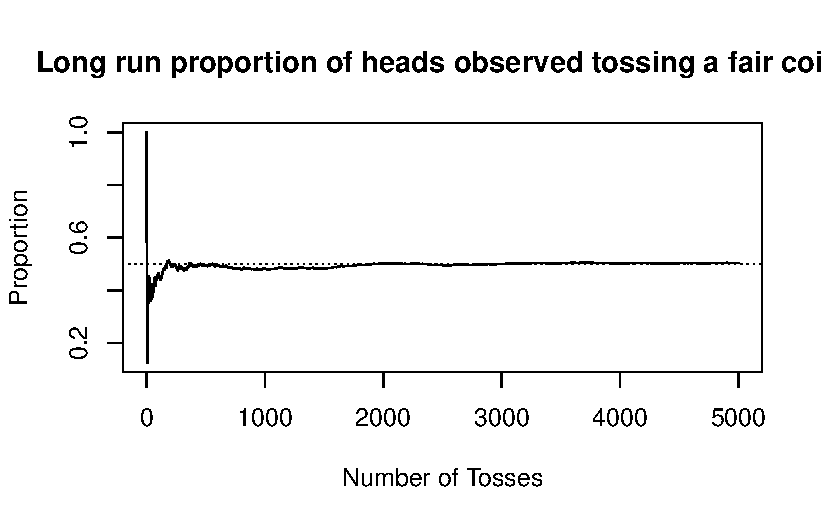
\includegraphics{notes/chapter1_files/figure-pdf/fig-plot-1.pdf}

}

\end{figure}%

To formalize this mathematically, we first define several important
terms.

\begin{definition}[Experiment]\protect\hypertarget{def-experiment}{}\label{def-experiment}

Any action to be performed whose outcome is not (or cannot) be known
with certainty, before it is performed.

\end{definition}

\begin{definition}[Event
{[}Informally{]}]\protect\hypertarget{def-event-inf}{}\label{def-event-inf}

A specified result that may or may not occur when an experiment is
performed.

\end{definition}

Suppose that an experiment is able to be performed as many times as one
likes, limited only by your boredom. If you take \(k_N\) to represent
the number of times that the event of interest occurs when you perform
the experiment \(N\) times, then a Frequentist would define the
probability of the event as
\[\text{probability} = \lim_{N\to\infty}\frac{k_N}{N}.\] This course
does not assume that you have any familiarity with calculus, and yet,
this definition relies on limits, a concept taken directly from
calculus. However, we will not actually require the ability to work with
limits for this course. Instead, when you see a statement of the form
\[\lim_{x\to\infty} f(x),\] simply think ``what is happening to the
function \(f(x)\) as \(x\) grows and grows (off to \(\infty\))?''

In practice this means that, in order to interpret probabilities, we
think about repeating an experiment many, many times over. As we do
that, we observe the proportion of times that any particular outcome
occurs, and take that to be the defining relation for probabilities. The
reason that we say the probability of flipping a heads is \(0.5\) is
because if we were to sit around and flip a coin\footnote{Our
  experiment.} over, and over, and over again, then in the long-run we
would observe a head\footnote{Our event.} in \(0.5\) of cases.

\begin{example}[Probability
Interpretation]\protect\hypertarget{exm-prob-interp}{}\label{exm-prob-interp}

How do we interpret the statement ``the probability that Sadie would
have had to pay, given a head on the first toss, is \(0.25\)''? Recall
that in the game, they toss three coins, and Sadie pays if two of them
show tails.

\begin{tcolorbox}[enhanced jigsaw, colback=white, breakable, rightrule=.15mm, leftrule=.75mm, toprule=.15mm, left=2mm, arc=.35mm, opacityback=0, bottomrule=.15mm]

\vspace{-3mm}\textbf{Solution}\vspace{3mm}

This statement means that, if Sadie were to repeatedly be in the
situation where one head has shown and there are two coins left to toss,
then in \(0.25\) of these situations (in the limit, as this is repeated
an infinite number of times) will end up showing two tails.

\end{tcolorbox}

\end{example}

Many situations in the real world are not able to be run over and over
again. Think about, for instance, the probability that a particular
candidate wins in a particular election. There is uncertainty there, of
course, but the election can only be run once. What then? There are
several ways through these types of events.

First, we can rely on the \textbf{power of imagination}. There is
nothing stopping us from envisioning the hypothetical possibility of
running the election over, and over, and over, and over again. If we
step outside of reality for a moment, we can ask ``if we could play the
day of the election many, many, many times, what proportion of those
days would end with the candidate being elected?'' If we say that the
candidate has a 75\% chance of being elected, then we mean that in
\(0.75\) of those imagined worlds, the candidate wins. It is crucial to
stress that in our imagination here, we need to be thinking about the
\textbf{exact same day} over and over again. We cannot imagine a
different path leading to the election, different speeches being given
in advance, or different opposition candidates. If we start from the
same place, and play it out many times over, what happens in each of
those worlds?

This repeated imagining is not for everyone. As a result, alternative
proposals to the interpretation of probability have been made. Most
popularly, the \textbf{Bayesian interpretation} has recently become
prominent. To Bayesians, probability is a measure of subjective belief.
To say that there is a \(50\%\) chance of a coin coming up is a
statement about one's knowledge of the world. Typically, coins show up
heads half the time, so that's our belief about heads. The Bayesian
view, built around subjective confidence in the state of the world, can
be formalized mathematically as well. A Bayesian considers the
\emph{prior evidence} that they have about the world\footnote{Any
  relevant evidence that has previously been collected.} and combine
this with current observations in order to update their subject beliefs,
balancing these two sources of information.

\begin{remark}[Bayesian Probabilities and Belief Updating]
Suppose that a Bayesian is flipping a coin. Before any flips have been
made the Bayesian understandably believes that the coin will come up
heads \(50\%\) of the time. However, when the coin starts to be flipped,
the observations are a string of tails in a row.

After having flipped the coin five times, the individual has observed
five tails. Of course, it is totally possible to flip a fair coin five
times and see five tails, but there is a level of skepticism growing.

After 10 flips, the Bayesian has still not seen a head. At this point,
the subjective belief is that there is likely something unfair about
this coin. Even though the experiment started with a baseline assumption
that the coin was fair the Bayesian no longer believes that the next
flip will be a head.

As this goes on, you can imagine the Bayesian continuing to update their
view of the world. To them, the probability is an evolving concept,
capturing what was believed and what has been observed.
\end{remark}

For the election example, the Bayesian interpretation is somewhat easier
to think through. To say that a candidate has a \(75\%\) chance of
winning the election means that ``based on everything that has been
observed, and any prior beliefs about the viability of the candidates,
the subjective likelihood that the candidate wins the election is
\(0.75\)''. If we disagree about prior beliefs, or have experienced
different pieces of information, then we may disagree on the
probability. That is okay.

In this course, we focus on the Frequentist interpretation. This is, in
part, because Frequentist probability is an easier introduction to the
concepts that are necessary for grasping uncertainty. Additionally,
there is some research to suggest that Frequentist interpretations are
fairly well understood by the general public \footnote{See, for instance
  Gigerenzer et al. (2005), where they study how people interpret the
  statement ``there is a \(30\%\) chance of rain tomorrow.''
  Interestingly, most people can convert this into a frequency statement
  (\(3\) out of \(10\), say), even if the specific meaning is sometimes
  lost. They conclude that there are other issues in attempting to
  understanding this statement, issues which we will address later on.}.
However, it is important to know and recognize that there is a world
beyond Frequentist Probability and Statistics, one which can be very
powerful once it is unlocked. \footnote{More on this in later years, if
  you so desire! Come have a chat, if that sounds interesting.}

If probability measures the long term proportion of times that a
particular event occurs, how can we go about computing probabilities? Do
we require to perform an experiment over and over again? Fortunately,
the answer is no. The tools of probability we will cover allow us to
make concrete statements about the probabilities of events without the
need for repeated experimental runs. However, before dismissing the idea
of repeatedly running an experiment at face value, it is worth
considering a tool we have at our disposal that renders this more
possible than it has ever been: computers.

\section{R Programming for Probability and
Statistics}\label{r-programming-for-probability-and-statistics}

Throughout this course we will make use of a programming language for
statistical computing, called R. Classically, introductory statistics
courses involved heavy computation of particular quantities by hand. The
use of a programming language (like R) frees us from the tedium of these
calculations, allowing for a deeper focus on understanding, explanation,
decision-making, and complex problem solving. This is \textbf{not} to
say we will \emph{never} do problems by hand\footnote{To the contrary,
  some amount of by-hand problem solving helps to solidify these
  concepts.}, however, we will emphasize the use of statistical
computing often. While you will not be expected to write R programs on
your own, you will be expected to read simple scripts, make basic
modifications, and to run code that is given to you.

Throughout these course notes, where relevant, R code will be provided
to demonstrate the ideas being discussed. It may be useful to have R
open alongside the notes to ensure that you can get the same results
that are printed throughout. In this section we will cover some of the
very basics of using R, and reading R code. If you are interested, there
are plenty of resources to becoming a more proficient R programmer. This
is a skill that will benefit you not only in this course, but in many
courses to come, and far beyond your university training. If you have
any programming in your background, R is a fairly simple language to
learn; if not, R can be quite beginner friendly.

\subsection{Basic Introduction to R
Programming}\label{basic-introduction-to-r-programming}

When programming, the basic idea is that we are going to write
instructions in a \textbf{script} which we will tell our computer to
execute. These instructions are\footnote{Typically. There are some
  exceptions to this, but if this is your first time programming, you
  need not worry about that!} performed one-by-one, from the top to the
bottom of the script. We can have instructions which operate on their
own, or which interact with previous (or future) instructions to add to
the complexity. The trick with programming then is to determine which
actions you need the computer to perform, in which order, to accomplish
the task that you are setting out to do.

To begin, we may consider a very simple R program, one which uses the
programming language as a basic calculator.

\begin{Shaded}
\begin{Highlighting}[]
\DecValTok{5} \SpecialCharTok{+} \DecValTok{3} \SpecialCharTok{{-}}\NormalTok{ (}\DecValTok{10}\SpecialCharTok{*}\DecValTok{2}\NormalTok{) }\SpecialCharTok{+} \DecValTok{8}\SpecialCharTok{\^{}}\NormalTok{(}\DecValTok{25}\SpecialCharTok{/}\DecValTok{3}\NormalTok{)}
\DocumentationTok{\#\# [1] 33554420}
\end{Highlighting}
\end{Shaded}

Here, we ask the computer to perform some simple arithmetic operations.
We use \texttt{+} for addition, \texttt{-} for subtraction, \texttt{*}
for multiplication, \texttt{/} for division, and \texttt{\^{}} for
exponentiation. With the use of parentheses, any expressions relating to
these basic operations can be performed. Note that here the result is
simply output after it is computed. Try modifying the exact expressions
being computed, allowing you to feel comfortable with these types of
mathematical operations.

\begin{Shaded}
\begin{Highlighting}[]
\DecValTok{5} \SpecialCharTok{+} \DecValTok{3} \SpecialCharTok{{-}}\NormalTok{ (}\DecValTok{10}\SpecialCharTok{*}\DecValTok{2}\NormalTok{) }\SpecialCharTok{+} \DecValTok{8}\SpecialCharTok{\^{}}\NormalTok{(}\DecValTok{25}\SpecialCharTok{/}\DecValTok{3}\NormalTok{)}
\DecValTok{8} \SpecialCharTok{*} \DecValTok{5}
\DocumentationTok{\#\# [1] 33554420}
\DocumentationTok{\#\# [1] 40}
\end{Highlighting}
\end{Shaded}

Here, we have two lines of math running with simple operations. Each is
simply output when it is computed. These two results have no ability to
interact with one another, and if we were to add more and more lines
beneath, the same would continue to happen. If we want different
commands to be able to interact with one another, we need a method for
storing the results. To do so, we can define \textbf{variables}. In R,
to define a variable, we use the syntax
\texttt{variable\_name\ \textless{}-\ variable\_value}. We can choose
\emph{almost} anything that we want for the variable name\footnote{The
  variable name must start with a letter and can be a combination of
  letters, numbers, periods, and underscore.} and the variable value can
also be of many types.\footnote{more on this later} The arrow between
the two is the \textbf{assignment operator} and it simply tells R to
assign the \texttt{variable\_value} to be accessible from the
\texttt{variable\_name}.

\begin{Shaded}
\begin{Highlighting}[]
\NormalTok{my\_5 }\OtherTok{\textless{}{-}} \DecValTok{5}
\NormalTok{my\_8 }\OtherTok{\textless{}{-}} \DecValTok{8}
\NormalTok{my\_5}
\NormalTok{my\_8}
\DocumentationTok{\#\# [1] 5}
\DocumentationTok{\#\# [1] 8}
\end{Highlighting}
\end{Shaded}

In this code we assign the variable \texttt{my\_5} to contain the value
5, and the variable \texttt{my\_8} to contain the value 8. We can output
these as expressions themselves, simply by typing the variable name.
Simply outputting these variables is not of particular interest,
however, we can use the variables in later statements by simply
including the variable name in them.

\begin{Shaded}
\begin{Highlighting}[]
\NormalTok{my\_5 }\OtherTok{\textless{}{-}} \DecValTok{5}
\NormalTok{my\_8 }\OtherTok{\textless{}{-}} \DecValTok{8}
\NormalTok{my\_5}\SpecialCharTok{*}\NormalTok{my\_8}
\DocumentationTok{\#\# [1] 40}
\end{Highlighting}
\end{Shaded}

Here, instead of simply outputting the variables, we multiply them
together. We could have used \texttt{5\ *\ 8} in this case for the same
result, however, we are afforded a lot more flexibility with this
approach. Much of this flexibility comes from our capacity to
\emph{change} the values of variables over time. Consider the following
script, and try to understand why the output is the way that it is.

\begin{Shaded}
\begin{Highlighting}[]
\NormalTok{my\_5 }\OtherTok{\textless{}{-}} \DecValTok{5}
\NormalTok{my\_8 }\OtherTok{\textless{}{-}} \DecValTok{8}
\NormalTok{my\_5}\SpecialCharTok{*}\NormalTok{my\_8}

\NormalTok{my\_5 }\OtherTok{\textless{}{-}} \DecValTok{10}
\NormalTok{my\_5}\SpecialCharTok{*}\NormalTok{my\_8}
\DocumentationTok{\#\# [1] 40}
\DocumentationTok{\#\# [1] 80}
\end{Highlighting}
\end{Shaded}

At the top point in the script, before the first \texttt{my\_5*my\_8}
call, The variable \texttt{my\_5} has the value \texttt{5}. However,
after this is called, the value is updated to be \texttt{10}. Then, when
we call \texttt{my\_5*my\_8} again, this is now simplified to
\texttt{10\ *\ 8}, giving the result. Perhaps more importantly, we can
take the value of an expression and assign that to a variable itself.

\begin{Shaded}
\begin{Highlighting}[]
\NormalTok{my\_5 }\OtherTok{\textless{}{-}} \DecValTok{5}
\NormalTok{my\_8 }\OtherTok{\textless{}{-}} \DecValTok{8}
\NormalTok{result }\OtherTok{\textless{}{-}}\NormalTok{ my\_5}\SpecialCharTok{*}\NormalTok{my\_8}
\NormalTok{result }
\DocumentationTok{\#\# [1] 40}
\end{Highlighting}
\end{Shaded}

Here, we define another variable. This time, \texttt{result} now
contains the result of multiplying our previous two variables. Thus,
when we output it, we get the same value. Take a moment to read through
the following script, and try to understand what will happen at the end.

\begin{Shaded}
\begin{Highlighting}[]
\NormalTok{my\_5 }\OtherTok{\textless{}{-}} \DecValTok{5}
\NormalTok{my\_8 }\OtherTok{\textless{}{-}} \DecValTok{8}
\NormalTok{result }\OtherTok{\textless{}{-}}\NormalTok{ my\_5}\SpecialCharTok{*}\NormalTok{my\_8}

\NormalTok{my\_5 }\OtherTok{\textless{}{-}}\NormalTok{ result}
\NormalTok{my\_8 }\OtherTok{\textless{}{-}}\NormalTok{ my\_5}
\NormalTok{result }\OtherTok{\textless{}{-}}\NormalTok{ my\_5 }\SpecialCharTok{*}\NormalTok{ my\_8}

\NormalTok{result }
\end{Highlighting}
\end{Shaded}

The result is 1600. Why? We can read through this step-by-step in order
to understand this. First we set our variables to have the values of
\texttt{5} and \texttt{8}. Then, \texttt{result} is made to be the
product of our two variables, which in this case is \texttt{40}. After
that, we set the value of \texttt{my\_5} to be the same as the value of
\texttt{result}, which gives \texttt{my\_5} equal to \texttt{40}. At
this point, \texttt{result} equals \texttt{40}, \texttt{my\_5} equals
\texttt{40}, and \texttt{my\_8} is equal to \texttt{8}. The next line
updates \texttt{my\_8} to be the same as the value of \texttt{my\_5},
which we just clarified was \texttt{40}. As a result, all of the
variables we have defined now take on the value of \texttt{40}. The
final line before output, \texttt{result\ \textless{}-\ my\_5\ *\ my\_8}
updates the value of \texttt{result} to be the product of the two
variables again, this time giving \texttt{40\ *\ 40} which gives 1600.

\subsection{Function Calls in R}\label{function-calls-in-r}

Up until this point we have simply used numerical operations and
variable assignment. While this allows R to serve as a very powerful
calculator, we often want computers to do much more than arithmetic. As
a result, we need to explore \textbf{functions} in R. A function is a
piece of code which takes in various arguments and outputs some value
(or values). Most of the way that we will use R in this course is
through the use of function calls.\footnote{Note: when you begin to
  write programs for yourself, a lot of your time will be spent writing
  custom functions. If this is of interest to you, I suggest looking
  into programming more! For this course we will not need to define our
  own functions, except perhaps ones that will be defined for you.} This
is exactly analogous to a mathematical function: it is simply some rule
which maps input to output. In fact, some of the most basic functions in
R are functions which relate to mathematical functions.

\phantomsection\label{annotated-cell-9}%
\begin{Shaded}
\begin{Highlighting}[]
\NormalTok{x }\OtherTok{\textless{}{-}} \DecValTok{10} 

\FunctionTok{exp}\NormalTok{(x) }\hspace*{\fill}\NormalTok{\circled{1}}
\FunctionTok{sqrt}\NormalTok{(x) }\hspace*{\fill}\NormalTok{\circled{2}}
\FunctionTok{log}\NormalTok{(x) }\hspace*{\fill}\NormalTok{\circled{3}}
\DocumentationTok{\#\# [1] 22026.47}
\DocumentationTok{\#\# [1] 3.162278}
\DocumentationTok{\#\# [1] 2.302585}
\end{Highlighting}
\end{Shaded}

\begin{description}
\tightlist
\item[\circled{1}]
Computes the exponential function applied to \texttt{x}, that is
\(e^x = e^{10}\).
\item[\circled{2}]
Computes the square root of \texttt{x}, that is
\(\sqrt{x} = \sqrt{10}\).
\item[\circled{3}]
Computes the natural logarithm of \texttt{x}, that is
\(\log(x) = \log(10)\).
\end{description}

The basic format of a function call will always be
\texttt{function\_name(param1,\ param2,\ ...)}. Each of these functions
required only a single parameter, however, there are some functions
which take more than one parameter. If we have decimal numbers, for
instance, we may wish to round them. To do so, we can use the
\texttt{round} function in R, which takes two parameters: the number we
wish to round, and how many digits we wish to keep.

\begin{Shaded}
\begin{Highlighting}[]
\NormalTok{unrounded\_value }\OtherTok{\textless{}{-}} \FloatTok{3.141592}
\NormalTok{rounded\_value }\OtherTok{\textless{}{-}} \FunctionTok{round}\NormalTok{(unrounded\_value, }\AttributeTok{digits =} \DecValTok{3}\NormalTok{)}

\NormalTok{rounded\_value}
\DocumentationTok{\#\# [1] 3.142}
\end{Highlighting}
\end{Shaded}

There are a few things to note about this sequence of function calls.
First, note that we assign the output of a function to a new variable.
This behaves exactly as we saw above with simple numeric calculations.
Next, consider that the output of the function\footnote{Which we have
  stored in the variable \texttt{rounded\_value}} has a value of
\(3.142\). That is: we rounded the value to \(3\) decimal points,
exactly as would be expected. The final part to note is that the second
parameter passed to the function call is \textbf{named}. That is,
instead of simply calling \texttt{round(unrounded\_value,\ 3)}, we have
\texttt{round(unrounded\_value,\ digits\ =\ 3)}. If you had made the
first call this would have worked perfectly.\footnote{Try it out to
  convince yourself!} However, R also provides the ability to pass in
parameter names alongside the parameter values with the syntax
\texttt{function\_name(param\_name\ =\ param\_value,\ ...)}. The benefit
to doing this is two-fold. First, it is easier to read what is
happening, especially for function calls that you have never seen
before. Second, it removes the need to have the parameters ordered
correctly. It is best practice to \textbf{always} include parameter
names where you can.

Now, you may be wondering ``how do you know what the parameter names
should be?'' The names are built-in to the different functions that you
are working with and so overtime you will become quite familiar with
them. However, at any point you can also run the command
\texttt{?function\_name}, replacing \texttt{function\_name} with the
name of a function you are interested in, to open documentation about
that function. There you will see not only the names of the different
parameters, but useful information regarding what the function does,
examples of how to call it, and so forth.

\begin{Shaded}
\begin{Highlighting}[]
\NormalTok{?round}
\end{Highlighting}
\end{Shaded}

When we run this code, we are given \emph{a lot} of information. We can
see the function name, the details, how it's called, and so forth. In
the \textbf{Arguments} section we get a list of all of the arguments we
can pass to the function, along with a description of them. In this case
we see that \texttt{round} can take a parameter called \texttt{x} for
the number to be rounded, and \texttt{digits} (which we have previously
seen).

\begin{Shaded}
\begin{Highlighting}[]
\NormalTok{unrounded\_value }\OtherTok{\textless{}{-}} \FloatTok{3.141592}
\NormalTok{rounded\_value }\OtherTok{\textless{}{-}} \FunctionTok{round}\NormalTok{(}\AttributeTok{digits =} \DecValTok{3}\NormalTok{, }\AttributeTok{x =}\NormalTok{ unrounded\_value)}

\NormalTok{rounded\_value}
\DocumentationTok{\#\# [1] 3.142}
\end{Highlighting}
\end{Shaded}

This code produces the exact same output, where now both parameters are
named. Specifically, we could read this function call as ``round the
value of \texttt{x} to have \texttt{digits} decimal points.'' If you had
instead written \texttt{round(3,\ unrounded\_value)}, you would get the
value \texttt{3}, since now we are rounding \texttt{3} to
\texttt{3.141592} decimal points.

\subsection{Moving Beyond Numeric
Data}\label{moving-beyond-numeric-data}

So far, everything that we have looked at has been numeric data. We have
seen integers, and decimals. You can have negative results, say by
taking \texttt{my\_var\ \textless{}-\ -5}. And while numbers are
frequently useful, we will require further types of data to write useful
computer programs. For this course we will focus on three additional
data types: textual data which (referred to as \textbf{strings}), true
and false binary data (referred to as \textbf{booleans}), and lists of
the same data type (referred to as \textbf{vectors}). They will behave
in much the same way as numeric data, with different functions and
techniques which can be applied to them.

To define a string of text, we simply encapsulate the text that we are
interested in within quotation marks (either single
\texttt{\textquotesingle{}} or double \texttt{"} quotation marks will
work).

\begin{Shaded}
\begin{Highlighting}[]
\NormalTok{first\_string }\OtherTok{\textless{}{-}} \StringTok{"This is a string."}
\NormalTok{second\_string }\OtherTok{\textless{}{-}} \StringTok{\textquotesingle{}This is also a string.\textquotesingle{}}

\NormalTok{first\_string}
\DocumentationTok{\#\# [1] "This is a string."}
\end{Highlighting}
\end{Shaded}

Two commonly used functions which rely on strings are \texttt{paste} and
\texttt{print}. Each will take in strings as input, and they do not need
to be named. The function \texttt{paste} can take in as many strings as
you would like. It will ``paste'' together all the strings provided,
creating a longer string out of these. The function \texttt{print} will
display the string that is passed as output. Until now we have been
running these programs in a way where all calls are displayed as output:
this will not always be the case, and so print can come in handy there.

\begin{Shaded}
\begin{Highlighting}[]
\NormalTok{my\_greeting }\OtherTok{\textless{}{-}} \StringTok{"Hello! Welcome to R programming,"}
\NormalTok{my\_name }\OtherTok{\textless{}{-}} \StringTok{"Dylan"}

\NormalTok{combined\_string }\OtherTok{\textless{}{-}} \FunctionTok{paste}\NormalTok{(my\_greeting, my\_name, }\StringTok{"!"}\NormalTok{)}
\FunctionTok{print}\NormalTok{(combined\_string)}
\DocumentationTok{\#\# [1] "Hello! Welcome to R programming, Dylan !"}
\end{Highlighting}
\end{Shaded}

Note that \texttt{paste} has several additional options which can be
investigated in the documentation for \texttt{paste}. This is only the
simplest use case for it. In general, strings are particularly helpful
when we wish to have output from the computer that will be human
readable. Where strings are largely for humans, booleans are largely for
computers.

Much of what computer programming entails is checking whether certain
conditions hold, and then taking different actions depending on what is
found. In order to do this, the computer needs a way to represent true
and false statements. In R, these are codified with the values
\texttt{TRUE} and \texttt{FALSE}. Note, the capital letters here make a
difference. You cannot use \texttt{true} or \texttt{True} or any other
combination thereof. More important than simply being able to specify
the values \texttt{TRUE} and \texttt{FALSE} directly is the ability to
detect whether certain statements are \texttt{TRUE} or \texttt{FALSE}.
For this we require comparison operators.

If we think of mathematical comparisons we can state whether two things
are equal, or not equal, and whether one thing is less than (or equal
to) or greater than (or equal to) another. We can run all of these same
checks in R.

\begin{itemize}
\tightlist
\item
  To check whether two quantities are equal you use
  \texttt{quantity\_1\ ==\ quantity\_2}. This statement will be
  \texttt{TRUE} if \texttt{quantity\_1} and \texttt{quantity\_2} are
  exactly the same, and will be \texttt{FALSE} otherwise.
\item
  To check whether two quantities are not equal, you can use
  \texttt{quantity\_1\ !=\ quantity\_2}. This statement will be
  \texttt{TRUE} if the quantities differ from one another.
\item
  To check whether one quantity is larger than another, you can use
  \texttt{quantity\_1\ \textgreater{}\ quantity\_2}. If you want to know
  whether it is greater than \emph{or} equal to, you can use
  \texttt{quantity\_1\ \textgreater{}=\ quantity\_2}.
\item
  To check whether one quantity is smaller than another, you can use
  \texttt{quantity\_1\ \textless{}\ quantity\_2}. If you want to know
  whether it is less than \emph{or} equal to, you can use
  \texttt{quantity\_1\ \textless{}=\ quantity\_2}.
\end{itemize}

\begin{Shaded}
\begin{Highlighting}[]
\DecValTok{5} \SpecialCharTok{==} \DecValTok{5} \CommentTok{\# TRUE}
\DecValTok{5} \SpecialCharTok{==} \DecValTok{6} \CommentTok{\# FALSE}

\DecValTok{5} \SpecialCharTok{!=} \DecValTok{5} \CommentTok{\# FALSE }
\DecValTok{5} \SpecialCharTok{!=} \DecValTok{6} \CommentTok{\# TRUE }

\DecValTok{5} \SpecialCharTok{\textgreater{}} \DecValTok{6} \CommentTok{\# FALSE}
\DecValTok{5} \SpecialCharTok{\textgreater{}} \DecValTok{5} \CommentTok{\# FALSE}

\DecValTok{5} \SpecialCharTok{\textgreater{}=} \DecValTok{6} \CommentTok{\# FALSE}
\DecValTok{5} \SpecialCharTok{\textgreater{}=} \DecValTok{5} \CommentTok{\# TRUE}

\DecValTok{5} \SpecialCharTok{\textless{}} \DecValTok{6} \CommentTok{\# TRUE}
\DecValTok{5} \SpecialCharTok{\textless{}} \DecValTok{5} \CommentTok{\# FALSE }

\DecValTok{5} \SpecialCharTok{\textless{}=} \DecValTok{6} \CommentTok{\# TRUE }
\DecValTok{5} \SpecialCharTok{\textless{}=} \DecValTok{5} \CommentTok{\# TRUE }
\DocumentationTok{\#\# [1] TRUE}
\DocumentationTok{\#\# [1] FALSE}
\DocumentationTok{\#\# [1] FALSE}
\DocumentationTok{\#\# [1] TRUE}
\DocumentationTok{\#\# [1] FALSE}
\DocumentationTok{\#\# [1] FALSE}
\DocumentationTok{\#\# [1] FALSE}
\DocumentationTok{\#\# [1] TRUE}
\DocumentationTok{\#\# [1] TRUE}
\DocumentationTok{\#\# [1] FALSE}
\DocumentationTok{\#\# [1] TRUE}
\DocumentationTok{\#\# [1] TRUE}
\end{Highlighting}
\end{Shaded}

There are two key points to note beyond this. First, we will of course
not normally compare two constants to one another. We already know that
\texttt{5==5} and so we would not need to check it. We can, however,
plug-in variables, perhaps with unknown values, and have the same types
of statements being made. Second, the checks for equality and inequality
also work with other data types (like strings).

\begin{Shaded}
\begin{Highlighting}[]
\NormalTok{string1 }\OtherTok{\textless{}{-}} \StringTok{"STRING1"}
\NormalTok{string2 }\OtherTok{\textless{}{-}} \StringTok{"STRING1"}
\NormalTok{string3 }\OtherTok{\textless{}{-}} \StringTok{"string1"}
\NormalTok{string4 }\OtherTok{\textless{}{-}} \StringTok{"5"}
\NormalTok{string5 }\OtherTok{\textless{}{-}} \StringTok{"5.3421"}
\NormalTok{num1 }\OtherTok{\textless{}{-}} \DecValTok{5}
\NormalTok{num2 }\OtherTok{\textless{}{-}} \DecValTok{1}
\NormalTok{num3 }\OtherTok{\textless{}{-}} \DecValTok{0}
\NormalTok{bool1 }\OtherTok{\textless{}{-}} \ConstantTok{TRUE} 
\NormalTok{bool2 }\OtherTok{\textless{}{-}} \ConstantTok{FALSE} 

\NormalTok{string1 }\SpecialCharTok{==}\NormalTok{ string2 }\CommentTok{\# TRUE}
\NormalTok{string1 }\SpecialCharTok{==}\NormalTok{ string3 }\CommentTok{\# FALSE }
\NormalTok{string2 }\SpecialCharTok{!=}\NormalTok{ string3 }\CommentTok{\# TRUE}
\NormalTok{string1 }\SpecialCharTok{!=}\NormalTok{ string4 }\CommentTok{\# TRUE }

\NormalTok{string4 }\SpecialCharTok{==}\NormalTok{ num1    }\CommentTok{\# TRUE }
\NormalTok{string1 }\SpecialCharTok{==}\NormalTok{ num2    }\CommentTok{\# FALSE}
\NormalTok{num1 }\SpecialCharTok{==}\NormalTok{ string5    }\CommentTok{\# FALSE}
\NormalTok{num2 }\SpecialCharTok{==}\NormalTok{ bool1      }\CommentTok{\# TRUE }
\NormalTok{bool2 }\SpecialCharTok{==}\NormalTok{ num3      }\CommentTok{\# TRUE }
\NormalTok{bool2 }\SpecialCharTok{==}\NormalTok{ num2      }\CommentTok{\# FALSE}
\DocumentationTok{\#\# [1] TRUE}
\DocumentationTok{\#\# [1] FALSE}
\DocumentationTok{\#\# [1] TRUE}
\DocumentationTok{\#\# [1] TRUE}
\DocumentationTok{\#\# [1] TRUE}
\DocumentationTok{\#\# [1] FALSE}
\DocumentationTok{\#\# [1] FALSE}
\DocumentationTok{\#\# [1] TRUE}
\DocumentationTok{\#\# [1] TRUE}
\DocumentationTok{\#\# [1] FALSE}
\end{Highlighting}
\end{Shaded}

The final checks may be slightly odd. Here we are comparing across
different types of data. When we do this R will automatically try to
convert from one type to the other. With strings and numbers this is not
too challenging. If they can be converted nicely between types, then
they are and the values are compared. Otherwise, R will conclude they
are not equal by default. For booleans, it is important to note that
\texttt{TRUE\ ==\ 1} and \texttt{FALSE\ ==\ 0}. We will often use these
values interchangeably.

The final data type that we will consider are vectors. Vectors store
many different values, of the same type, in a single object. Thus, we
may have a vector of numeric data, or a vector of strings, or a vector
of booleans. The vectors will always contain the same type throughout,
but they are stored in a single object (and as such, for instance, can
be stored in a single variable). To define a vector we call
\texttt{c(...)}, where the \texttt{...} contains the set of objects we
want to store in the vector. The \texttt{c} stands for
\textbf{c}oncatenate, as we are \emph{concatenating} together the set of
items into a single container.

\begin{Shaded}
\begin{Highlighting}[]
\NormalTok{v1 }\OtherTok{\textless{}{-}} \FunctionTok{c}\NormalTok{(}\StringTok{"vector"}\NormalTok{, }\StringTok{"of"}\NormalTok{, }\StringTok{"strings"}\NormalTok{)}
\NormalTok{v2 }\OtherTok{\textless{}{-}} \FunctionTok{c}\NormalTok{(}\DecValTok{3}\NormalTok{, }\DecValTok{1}\NormalTok{, }\DecValTok{4}\NormalTok{, }\DecValTok{1}\NormalTok{, }\DecValTok{5}\NormalTok{)}
\NormalTok{v3 }\OtherTok{\textless{}{-}} \FunctionTok{c}\NormalTok{(}\ConstantTok{TRUE}\NormalTok{, }\ConstantTok{TRUE}\NormalTok{, }\ConstantTok{FALSE}\NormalTok{, }\ConstantTok{TRUE}\NormalTok{)}
\NormalTok{v4 }\OtherTok{\textless{}{-}} \FunctionTok{c}\NormalTok{(}\DecValTok{1}\SpecialCharTok{==}\DecValTok{2}\NormalTok{, }\DecValTok{2}\SpecialCharTok{==}\DecValTok{2}\NormalTok{, }\DecValTok{3}\SpecialCharTok{==}\DecValTok{4}\NormalTok{)}
\NormalTok{v1}
\NormalTok{v2}
\NormalTok{v3}
\NormalTok{v4}
\DocumentationTok{\#\# [1] "vector"  "of"      "strings"}
\DocumentationTok{\#\# [1] 3 1 4 1 5}
\DocumentationTok{\#\# [1]  TRUE  TRUE FALSE  TRUE}
\DocumentationTok{\#\# [1] FALSE  TRUE FALSE}
\end{Highlighting}
\end{Shaded}

We see that each of these vectors holds one type of object. Vectors can
be of arbitrary and different lengths. It is also possible to combine
multiple vectors \emph{of the same type} into one, by using the
\texttt{c} function again.

\begin{Shaded}
\begin{Highlighting}[]
\NormalTok{v1 }\OtherTok{\textless{}{-}} \FunctionTok{c}\NormalTok{(}\DecValTok{3}\NormalTok{,}\DecValTok{1}\NormalTok{,}\DecValTok{4}\NormalTok{,}\DecValTok{1}\NormalTok{,}\DecValTok{5}\NormalTok{)}
\NormalTok{v2 }\OtherTok{\textless{}{-}} \FunctionTok{c}\NormalTok{(}\DecValTok{9}\NormalTok{,}\DecValTok{2}\NormalTok{,}\DecValTok{6}\NormalTok{)}
\NormalTok{v3 }\OtherTok{\textless{}{-}} \FunctionTok{c}\NormalTok{(}\DecValTok{5}\NormalTok{)}
\NormalTok{num1 }\OtherTok{\textless{}{-}} \DecValTok{3}

\NormalTok{combined\_v1 }\OtherTok{\textless{}{-}} \FunctionTok{c}\NormalTok{(v1, v2)}
\NormalTok{combined\_v2 }\OtherTok{\textless{}{-}} \FunctionTok{c}\NormalTok{(combined\_v1, v3)}
\NormalTok{combined\_v3 }\OtherTok{\textless{}{-}} \FunctionTok{c}\NormalTok{(combined\_v2, num1)}

\NormalTok{combined\_v3}
\DocumentationTok{\#\#  [1] 3 1 4 1 5 9 2 6 5 3}
\end{Highlighting}
\end{Shaded}

Here we combine different numeric vectors together. We also show, when
forming \texttt{combined\_v3}, how numeric vectors can have single items
added onto them. That is, if you have a single number, it can be treated
as a vector with one element in it. This becomes very useful when
building up vectors within code. In addition to combining multiple
vectors together, we can also select elements out of a vector. To do
this, we use a set of square brackets after the vector's name, with a
number within those square brackets specifying the \textbf{index} of the
vector we are interested in. The index is simply the element position
starting at 1\footnote{If you have programmed in the past there is a
  good chance the language you have learned is ``0 indexed'' rather than
  ``1 indexed''. In R, all vectors start at position 1 and count up,
  which is not the case in many languages. Be careful of this.} and
running to the length of the vector. We can include a vector of indices
to select multiple elements at once.

\begin{Shaded}
\begin{Highlighting}[]
\NormalTok{alpha\_vector }\OtherTok{\textless{}{-}} \FunctionTok{c}\NormalTok{(}\StringTok{"A"}\NormalTok{,}\StringTok{"B"}\NormalTok{,}\StringTok{"C"}\NormalTok{,}\StringTok{"D"}\NormalTok{,}\StringTok{"E"}\NormalTok{,}\StringTok{"F"}\NormalTok{,}\StringTok{"G"}\NormalTok{,}\StringTok{"H"}\NormalTok{,}\StringTok{"I"}\NormalTok{,}
                  \StringTok{"J"}\NormalTok{,}\StringTok{"K"}\NormalTok{,}\StringTok{"L"}\NormalTok{,}\StringTok{"M"}\NormalTok{,}\StringTok{"N"}\NormalTok{,}\StringTok{"O"}\NormalTok{,}\StringTok{"P"}\NormalTok{,}\StringTok{"Q"}\NormalTok{,}\StringTok{"R"}\NormalTok{,}
                  \StringTok{"S"}\NormalTok{,}\StringTok{"T"}\NormalTok{,}\StringTok{"U"}\NormalTok{,}\StringTok{"V"}\NormalTok{,}\StringTok{"W"}\NormalTok{,}\StringTok{"X"}\NormalTok{,}\StringTok{"Y"}\NormalTok{,}\StringTok{"Z"}\NormalTok{)}

\NormalTok{alpha\_vector[}\DecValTok{4}\NormalTok{]    }\CommentTok{\# D}
\NormalTok{alpha\_vector[}\DecValTok{25}\NormalTok{]   }\CommentTok{\# Y }
\NormalTok{alpha\_vector[}\DecValTok{12}\NormalTok{]   }\CommentTok{\# L}
\NormalTok{alpha\_vector[}\DecValTok{1}\NormalTok{]    }\CommentTok{\# A}
\NormalTok{alpha\_vector[}\DecValTok{14}\NormalTok{]   }\CommentTok{\# N}

\NormalTok{my\_name }\OtherTok{\textless{}{-}}\NormalTok{ alpha\_vector[}\FunctionTok{c}\NormalTok{(}\DecValTok{4}\NormalTok{,}\DecValTok{25}\NormalTok{,}\DecValTok{12}\NormalTok{,}\DecValTok{1}\NormalTok{,}\DecValTok{14}\NormalTok{)]}

\NormalTok{my\_name }
\DocumentationTok{\#\# [1] "D"}
\DocumentationTok{\#\# [1] "Y"}
\DocumentationTok{\#\# [1] "L"}
\DocumentationTok{\#\# [1] "A"}
\DocumentationTok{\#\# [1] "N"}
\DocumentationTok{\#\# [1] "D" "Y" "L" "A" "N"}
\end{Highlighting}
\end{Shaded}

Note that, each element is selectable individually, giving a single item
of that type (in this case, strings). If you select multiple of the
elements together, it will create a vector of that type (in this case, a
string vector). Note that in addition to selecting elements in this way
by their indices, you can also update the elements in the same way.

\begin{Shaded}
\begin{Highlighting}[]
\NormalTok{cur\_year }\OtherTok{\textless{}{-}} \FunctionTok{c}\NormalTok{(}\DecValTok{2}\NormalTok{,}\DecValTok{0}\NormalTok{,}\DecValTok{2}\NormalTok{,}\DecValTok{3}\NormalTok{)}
\NormalTok{cur\_year }

\CommentTok{\# After Midnight on December 31}
\NormalTok{cur\_year[}\DecValTok{4}\NormalTok{] }\OtherTok{\textless{}{-}} \DecValTok{4}
\NormalTok{cur\_year }
\DocumentationTok{\#\# [1] 2 0 2 3}
\DocumentationTok{\#\# [1] 2 0 2 4}
\end{Highlighting}
\end{Shaded}

In this example we are changing the last element of the vector.
Sometimes we may not know how long the vector actually is, if for
instance, it is being built-up as our code runs. If we ever want to
check the length of a vector, we can simply call the function
\texttt{length} which takes as input only one vector, and outputs the
numeric value of its length.

\begin{Shaded}
\begin{Highlighting}[]
\NormalTok{v1 }\OtherTok{\textless{}{-}} \FunctionTok{c}\NormalTok{(}\DecValTok{1}\NormalTok{,}\DecValTok{2}\NormalTok{,}\DecValTok{3}\NormalTok{,}\DecValTok{4}\NormalTok{,}\DecValTok{5}\NormalTok{)}
\FunctionTok{length}\NormalTok{(v1)}
\DocumentationTok{\#\# [1] 5}
\end{Highlighting}
\end{Shaded}

\subsection{Program Control Flow}\label{program-control-flow}

We have seen different types of data, different ways of manipulating
data, functions, and variables so far. In order to bring all of these
concepts together into useful programs we need some way to control the
flow of our programs. We have seen that, by default, programs execute
from the top until the bottom. However, it will often be the case that
we want want to have certain code running only if certain conditions
hold, or that we want to repeat some piece of code many times over. To
accomplish these tasks we require \textbf{control flow statements}. We
will consider only two types of control flow statements now, which will
serve well enough to read most of what needs to be read for this course.

The first type of statement is the \textbf{conditional statement}.
Conditional statements execute only when certain conditions hold. The
simplest conditional statement is an \textbf{if} statement. The format
to define an if statement if \texttt{if\ (condition)\{\ ...\ \}}, where
\texttt{condition} is some logical condition to be evaluated. If the
condition is \texttt{TRUE} then the code contained in \{ \ldots{} \} is
evaluated. If the condition is \texttt{FALSE} it is not.

\begin{Shaded}
\begin{Highlighting}[]
\NormalTok{my\_number }\OtherTok{\textless{}{-}} \DecValTok{5}

\ControlFlowTok{if}\NormalTok{(my\_number }\SpecialCharTok{\textgreater{}} \DecValTok{0}\NormalTok{) \{}
    \FunctionTok{print}\NormalTok{(}\StringTok{"My number is a positive."}\NormalTok{)}
\NormalTok{\}}

\ControlFlowTok{if}\NormalTok{(my\_number }\SpecialCharTok{\textless{}} \DecValTok{0}\NormalTok{) \{}
    \FunctionTok{print}\NormalTok{(}\StringTok{"My number is a negative."}\NormalTok{)}
\NormalTok{\}}
\DocumentationTok{\#\# [1] "My number is a positive."}
\end{Highlighting}
\end{Shaded}

In this case, these simple conditional statement check to see whether
the number we entered is larger than zero and whether the number we
entered is smaller than zero, respectively. When run, notice that only
one of the statements is executed.\footnote{In fact, if
  \texttt{my\_number} is set to \texttt{0} then none of the statements
  are executed.} In this case, we know that only one (or neither) of
these statements can be true. When that is the case it may make sense to
make use of \texttt{else} clauses in our conditional logic.

\begin{Shaded}
\begin{Highlighting}[]
\NormalTok{my\_number }\OtherTok{\textless{}{-}} \SpecialCharTok{{-}}\DecValTok{5}

\ControlFlowTok{if}\NormalTok{(my\_number }\SpecialCharTok{\textgreater{}} \DecValTok{0}\NormalTok{) \{}
    \FunctionTok{print}\NormalTok{(}\StringTok{"My number is a positive."}\NormalTok{)}
\NormalTok{\} }\ControlFlowTok{else}\NormalTok{ \{}
    \FunctionTok{print}\NormalTok{(}\StringTok{"My number is not a positive."}\NormalTok{)}
\NormalTok{\}}
\DocumentationTok{\#\# [1] "My number is not a positive."}
\end{Highlighting}
\end{Shaded}

Here, \emph{if} the number is greater than \texttt{0}, then we run the
first block of code, \emph{otherwise} we run the second block of code.
Thus, whenever a positive number is entered, we see ``My number is a
positive'', and whenever a non-positive number is entered, we see ``My
number is not a positive.'' We can extend \texttt{else} blocks to be
\texttt{else\ if} blocks, where further conditions can be specified.

\begin{Shaded}
\begin{Highlighting}[]
\NormalTok{my\_number }\OtherTok{\textless{}{-}} \DecValTok{100}

\ControlFlowTok{if}\NormalTok{(my\_number }\SpecialCharTok{\textgreater{}} \DecValTok{50}\NormalTok{) \{}
    \FunctionTok{print}\NormalTok{(}\StringTok{"My number is a large positive value."}\NormalTok{)}
\NormalTok{\} }\ControlFlowTok{else} \ControlFlowTok{if}\NormalTok{(my\_number }\SpecialCharTok{\textgreater{}} \DecValTok{0}\NormalTok{)\{}
    \FunctionTok{print}\NormalTok{(}\StringTok{"My number is a small positive value."}\NormalTok{)}
\NormalTok{\} }\ControlFlowTok{else} \ControlFlowTok{if}\NormalTok{(my\_number }\SpecialCharTok{\textless{}} \SpecialCharTok{{-}}\DecValTok{50}\NormalTok{) \{}
    \FunctionTok{print}\NormalTok{(}\StringTok{"My number is a large negative value."}\NormalTok{)}
\NormalTok{\} }\ControlFlowTok{else} \ControlFlowTok{if}\NormalTok{(my\_number }\SpecialCharTok{\textless{}} \DecValTok{0}\NormalTok{) \{}
    \FunctionTok{print}\NormalTok{(}\StringTok{"My number is a small negative value."}\NormalTok{)}
\NormalTok{\} }\ControlFlowTok{else}\NormalTok{ \{}
    \FunctionTok{print}\NormalTok{(}\StringTok{"My number is zero."}\NormalTok{)}
\NormalTok{\}}
\DocumentationTok{\#\# [1] "My number is a large positive value."}
\end{Highlighting}
\end{Shaded}

In these case we can simply pass through each conditional statement in
order. First, is the number larger than \texttt{50}? If so, print the
statement, otherwise we check the next condition, is the number greater
than \texttt{0}? Note that if we are checking this condition we
\emph{know} that the number is less than or equal to \texttt{50} since
it failed the first check. We continue through the rest of this
procedure down until the last else block. This block is run only when
all of the other conditions fail: that is, our value is not larger than
\texttt{50}, or larger than \texttt{0}, or smaller than \texttt{-50}, or
smaller than \texttt{0}. The only value that satisfies this is
\texttt{0} itself.

Sometimes, we wish to check compound conditions. That is, we want to
know whether multiple conditions hold, or perhaps, whether at least one
of many conditions hold. These statements can be converted into ``and''
and ``or'' statements, respectively. To denote ``and'' statements we use
\texttt{\&\&} and to denote ``or'' statements we use
\texttt{\textbar{}\textbar{}}. Thus, the check
\texttt{my\_val\ \textgreater{}\ 0\ \&\&\ my\_val\ \textless{}\ 100}
returns true only if \texttt{my\_val} is both above \texttt{0}
\textbf{and} below 100. The check
\texttt{my\_val\ \textless{}\ -50\ \textbar{}\textbar{}\ my\_val\ \textgreater{}\ 50}
returns true whenever \textbf{either} \texttt{my\_val} is less than
\texttt{-50} \textbf{or} \texttt{my\_val} is greater than \texttt{50}.

\begin{Shaded}
\begin{Highlighting}[]
\NormalTok{my\_number }\OtherTok{\textless{}{-}} \DecValTok{5}

\ControlFlowTok{if}\NormalTok{(my\_number }\SpecialCharTok{\textless{}} \DecValTok{50} \SpecialCharTok{\&\&}\NormalTok{ my\_number }\SpecialCharTok{\textgreater{}} \DecValTok{10}\NormalTok{) \{}
    \FunctionTok{print}\NormalTok{(}\StringTok{"A moderate, positive number."}\NormalTok{)}
\NormalTok{\} }\ControlFlowTok{else} \ControlFlowTok{if}\NormalTok{(my\_number }\SpecialCharTok{!=} \DecValTok{5} \SpecialCharTok{\&\&}\NormalTok{ my\_number }\SpecialCharTok{\textless{}=} \DecValTok{10} \SpecialCharTok{\&\&}\NormalTok{ my\_number }\SpecialCharTok{\textgreater{}=} \DecValTok{0}\NormalTok{) \{}
    \FunctionTok{print}\NormalTok{(}\StringTok{"A positive value which is not 5."}\NormalTok{)}
\NormalTok{\} }\ControlFlowTok{else} \ControlFlowTok{if}\NormalTok{(my\_number }\SpecialCharTok{==} \DecValTok{5} \SpecialCharTok{||}\NormalTok{ my\_number }\SpecialCharTok{\textless{}} \DecValTok{0}\NormalTok{) \{}
    \FunctionTok{print}\NormalTok{(}\StringTok{"Either 5 or a negative value."}\NormalTok{)}
\NormalTok{\}}
\DocumentationTok{\#\# [1] "Either 5 or a negative value."}
\end{Highlighting}
\end{Shaded}

Conditional statements can grow to be very complex, however, with these
rules you can read through them top-to-bottom, substituting for ``and''
and ``or'' where necessary. It is also possible, where required, to
place one conditional statement inside the code block for another, and
to combine them with any of the other techniques that we have learned
thus far.

The final piece of control flow that we will consider for now is the
\texttt{for} loop. The idea with a \texttt{for} loop is that we want to
repeat the same action either a certain number of times, or for every
item in a set of items. To do so, we use the syntax
\texttt{for(x\ in\ vector)\{...\}}, where the code in \texttt{...} will
be performed once for every single item in the vector. Within the code
block specified by \texttt{...}, the value \texttt{x} will take on the
current value in the loop.

\begin{Shaded}
\begin{Highlighting}[]
\ControlFlowTok{for}\NormalTok{(x }\ControlFlowTok{in} \FunctionTok{c}\NormalTok{(}\DecValTok{1}\NormalTok{,}\DecValTok{2}\NormalTok{,}\DecValTok{3}\NormalTok{))\{}
    \FunctionTok{print}\NormalTok{(x)}
\NormalTok{\}}
\DocumentationTok{\#\# [1] 1}
\DocumentationTok{\#\# [1] 2}
\DocumentationTok{\#\# [1] 3}
\end{Highlighting}
\end{Shaded}

Notice that three values are printed, in order, \texttt{1} then
\texttt{2} then \texttt{3}. The loop code is run three different times,
one for each element in the list. Each time the loop is running the next
value from the list gets assigned to the variable \texttt{x}. The first
time it runs it gets the first element, and so forth. As a result, we
can use these values in our calculations in whatever way we need to.

\begin{Shaded}
\begin{Highlighting}[]
\ControlFlowTok{for}\NormalTok{(x }\ControlFlowTok{in} \FunctionTok{c}\NormalTok{(}\DecValTok{1}\NormalTok{,}\DecValTok{2}\NormalTok{,}\DecValTok{3}\NormalTok{))\{}
\NormalTok{    x\_sq }\OtherTok{\textless{}{-}}\NormalTok{ x}\SpecialCharTok{\^{}}\DecValTok{2}
    \FunctionTok{print}\NormalTok{(}\FunctionTok{paste}\NormalTok{(}\StringTok{"The square of"}\NormalTok{, x, }\StringTok{\textquotesingle{}is\textquotesingle{}}\NormalTok{, x\_sq))}
\NormalTok{\}}
\DocumentationTok{\#\# [1] "The square of 1 is 1"}
\DocumentationTok{\#\# [1] "The square of 2 is 4"}
\DocumentationTok{\#\# [1] "The square of 3 is 9"}
\end{Highlighting}
\end{Shaded}

Whenever we are trying to form a numeric vector with consecutive
elements, as we are in \texttt{c(1,2,3)}, we can make this easier on
ourselves by simply specifying the upper and lower bounds of the range,
separated by a colon. That is \texttt{c(1,2,3)\ ==\ 1:3}. This is often
useful when specify a loop as we very often want to repeat something a
set number of times. Note that we do not ever \emph{need} to use the
value of the looping variable. Sometimes, we just want things to repeat,
and so the loop is a convenient way to do that.

\begin{Shaded}
\begin{Highlighting}[]
\NormalTok{times\_to\_loop }\OtherTok{\textless{}{-}} \DecValTok{5}

\ControlFlowTok{for}\NormalTok{(x }\ControlFlowTok{in} \DecValTok{1}\SpecialCharTok{:}\NormalTok{times\_to\_loop)\{}
    \FunctionTok{print}\NormalTok{(}\FunctionTok{paste}\NormalTok{(}\StringTok{"This will get printed"}\NormalTok{, times\_to\_loop, }\StringTok{"times."}\NormalTok{))}
\NormalTok{\}}
\DocumentationTok{\#\# [1] "This will get printed 5 times."}
\DocumentationTok{\#\# [1] "This will get printed 5 times."}
\DocumentationTok{\#\# [1] "This will get printed 5 times."}
\DocumentationTok{\#\# [1] "This will get printed 5 times."}
\DocumentationTok{\#\# [1] "This will get printed 5 times."}
\end{Highlighting}
\end{Shaded}

\subsection{Reading Through a More Complex R
Program}\label{reading-through-a-more-complex-r-program}

Take a moment to read through the following R program and try to
understand what is happening exactly. There are comments throughout
which will assist in the parsing of the script. We have seen comments up
until now, without drawing explicit attention to them. In R, anything
placed after a \texttt{\#} on the line is considered a comment. The
programming language ignores these and so they are only there to help
other individuals who may be reading through. It is good practice to
comment your code to help others, and also to help yourself whenever you
return to it in the future. In the course notes code will typically be
commented. If you are reading the PDF version of the notes often these
comments will be annotations beside the code (numbering certain lines)
with the comments provided below, for the sake of legibility.

Note, this combines everything that we have learned, and it is entirely
understandable if it takes some time to process. Fortunately, you can
always try running the script yourself, and playing with different
components of it. Remember, if you do not know what a function call
does, you can use the documentation\footnote{The internet is also a
  wonderful resource, one which even very experienced developers make
  frequent use of.} and try playing with it some yourself. To help with
the interpretation here, note that this is an implementation of the game
that Charles and Sadie have been playing.

\begin{Shaded}
\begin{Highlighting}[]
\CommentTok{\# Define some variables which dictate how the game runs.}
\NormalTok{player1 }\OtherTok{\textless{}{-}} \StringTok{"Charles"}
\NormalTok{player2 }\OtherTok{\textless{}{-}} \StringTok{"Sadie"}
\NormalTok{num\_of\_flips }\OtherTok{\textless{}{-}} \DecValTok{3}
\NormalTok{flip\_option1 }\OtherTok{\textless{}{-}} \StringTok{"H"}
\NormalTok{flip\_option2 }\OtherTok{\textless{}{-}} \StringTok{"T"}

\CommentTok{\# Begin with the game setup}
\NormalTok{num\_to\_win }\OtherTok{\textless{}{-}} \FunctionTok{round}\NormalTok{(}\AttributeTok{x =}\NormalTok{ num\_of\_flips }\SpecialCharTok{/} \DecValTok{2}\NormalTok{, }\DecValTok{0}\NormalTok{)}
\NormalTok{flip\_results }\OtherTok{\textless{}{-}} \FunctionTok{c}\NormalTok{()}
\NormalTok{flip\_options }\OtherTok{\textless{}{-}} \FunctionTok{c}\NormalTok{(flip\_option1, flip\_option2)}
\NormalTok{total\_1 }\OtherTok{\textless{}{-}} \DecValTok{0}
\NormalTok{total\_2 }\OtherTok{\textless{}{-}} \DecValTok{0}
\NormalTok{player\_name }\OtherTok{\textless{}{-}} \StringTok{""} \CommentTok{\# This is an \textquotesingle{}empty string\textquotesingle{}}

\CommentTok{\# Start Playing the Game}
\ControlFlowTok{for}\NormalTok{(game\_round }\ControlFlowTok{in} \DecValTok{1}\SpecialCharTok{:}\NormalTok{num\_of\_flips) \{}
    \FunctionTok{print}\NormalTok{(}\FunctionTok{paste}\NormalTok{(}\StringTok{"Now starting round"}\NormalTok{, game\_round))}

    \CommentTok{\# Select a flip of the coin, using the sample function.}
    \CommentTok{\# See more details with ?sample}
\NormalTok{    flip\_result }\OtherTok{\textless{}{-}} \FunctionTok{sample}\NormalTok{(}\AttributeTok{x =}\NormalTok{ flip\_options, }\AttributeTok{size =} \DecValTok{1}\NormalTok{)}

    \CommentTok{\# See who benefits from this flip}
    \CommentTok{\# Then set player\_name to be the player who benefits from the flip,}
    \CommentTok{\# and update their score variable.}
    \ControlFlowTok{if}\NormalTok{ (flip\_result }\SpecialCharTok{==}\NormalTok{ flip\_option1) \{}
\NormalTok{        player\_name }\OtherTok{\textless{}{-}}\NormalTok{ player1}
\NormalTok{        total\_1 }\OtherTok{\textless{}{-}}\NormalTok{ total\_1 }\SpecialCharTok{+} \DecValTok{1}
\NormalTok{    \} }\ControlFlowTok{else} \ControlFlowTok{if}\NormalTok{ (flip\_result }\SpecialCharTok{==}\NormalTok{ flip\_option2) \{}
\NormalTok{        player\_name }\OtherTok{\textless{}{-}}\NormalTok{ player2}
\NormalTok{        total\_2 }\OtherTok{\textless{}{-}}\NormalTok{ total\_2 }\SpecialCharTok{+} \DecValTok{1}
\NormalTok{    \}}

    \FunctionTok{print}\NormalTok{(}\FunctionTok{paste}\NormalTok{(}\StringTok{"The flip was a"}\NormalTok{, flip\_result, }\StringTok{"which benefits"}\NormalTok{, player\_name))}

    \CommentTok{\# Check to see if either player has won at this point.}
    \ControlFlowTok{if}\NormalTok{(total\_1 }\SpecialCharTok{\textgreater{}=}\NormalTok{ num\_to\_win) \{}
        \FunctionTok{print}\NormalTok{(}\FunctionTok{paste}\NormalTok{(player1, }\StringTok{"has scored enough points to win."}\NormalTok{))}
\NormalTok{    \} }\ControlFlowTok{else} \ControlFlowTok{if}\NormalTok{(total\_2 }\SpecialCharTok{\textgreater{}=}\NormalTok{ num\_to\_win)\{}
        \FunctionTok{print}\NormalTok{(}\FunctionTok{paste}\NormalTok{(player2, }\StringTok{"has scored enough points to win."}\NormalTok{))}
\NormalTok{    \}}
\NormalTok{\}}

\CommentTok{\# The game is over}
\CommentTok{\# Select the winner based on who scored above the threshold }
\CommentTok{\# and then print out the results.}
\NormalTok{winner }\OtherTok{\textless{}{-}}\NormalTok{ player1 }

\ControlFlowTok{if}\NormalTok{(total\_2 }\SpecialCharTok{\textgreater{}=}\NormalTok{ num\_to\_win) \{}
\NormalTok{    winner }\OtherTok{\textless{}{-}}\NormalTok{ player2 }
\NormalTok{\}}

\CommentTok{\# Separate these statements into multiple lines to ensure the text is }
\CommentTok{\# not too wide.}
\FunctionTok{print}\NormalTok{(}\FunctionTok{paste}\NormalTok{(}\StringTok{"After flipping the coin"}\NormalTok{, num\_of\_flips, }\StringTok{"times,"}\NormalTok{, player1, }
            \StringTok{"scored a total of"}\NormalTok{, total\_1, }\StringTok{"points"}\NormalTok{))}
\FunctionTok{print}\NormalTok{(}\FunctionTok{paste}\NormalTok{(}\StringTok{"while"}\NormalTok{, player2, }\StringTok{"scored a total of"}\NormalTok{, total\_2, }\StringTok{"points."}\NormalTok{))}
\FunctionTok{print}\NormalTok{(}\FunctionTok{paste}\NormalTok{(}\StringTok{"As a result"}\NormalTok{, winner, }\StringTok{"won the game and will not have to pay!"}\NormalTok{))}
\DocumentationTok{\#\# [1] "Now starting round 1"}
\DocumentationTok{\#\# [1] "The flip was a H which benefits Charles"}
\DocumentationTok{\#\# [1] "Now starting round 2"}
\DocumentationTok{\#\# [1] "The flip was a T which benefits Sadie"}
\DocumentationTok{\#\# [1] "Now starting round 3"}
\DocumentationTok{\#\# [1] "The flip was a T which benefits Sadie"}
\DocumentationTok{\#\# [1] "Sadie has scored enough points to win."}
\DocumentationTok{\#\# [1] "After flipping the coin 3 times, Charles scored a total of 1 points"}
\DocumentationTok{\#\# [1] "while Sadie scored a total of 2 points."}
\DocumentationTok{\#\# [1] "As a result Sadie won the game and will not have to pay!"}
\end{Highlighting}
\end{Shaded}

\subsection{R Programming for Probability
Interpretations}\label{r-programming-for-probability-interpretations}

Recall that the motivation for the discussion of R was the Frequentist
interpretation of probability. One task that computers are very
effective at is repeatedly performing some action. As a result, we can
use computers to mimic the idea of repeatedly performing an experiment.
Consider the simple case of flipping a coin over and over again.

We can use \texttt{sample(x,\ size)} as a function to select
\texttt{size} realizations from the set contained in \texttt{x}. Thus,
if we take \texttt{sample(x\ =\ c("H","T"),\ size=1)} we can view this
as flipping a coin one time. If we use the loop structure we talked
before, then we can simulate the experience of repeatedly flipping a
coin. Consider the following R code. Note, any time that we are doing
something which is randomized in R (such as drawing random samples) we
also will make use of the \texttt{set.seed()} function. This function
takes in an integer value as an argument, and by providing the
\emph{same} integer value we can make sure to always get the same random
numbers generated.\footnote{Technically, we cannot use a computer to
  generate random numbers. We can only generate \emph{pseudo random}
  numbers, which are close enough for most purposes.} This helps to
ensure the repeatability of any R analysis, and it is good practice to
do. To see what happens without seeding, try modifying the following
code without a seed, and running it several times. Then, set the seed
(to any number you like) and do the same process.

\phantomsection\label{annotated-cell-30}%
\begin{Shaded}
\begin{Highlighting}[]
\FunctionTok{set.seed}\NormalTok{(}\DecValTok{3141592}\NormalTok{) }\hspace*{\fill}\NormalTok{\circled{1}}

\NormalTok{number\_of\_runs }\OtherTok{\textless{}{-}} \DecValTok{1000} \hspace*{\fill}\NormalTok{\circled{2}}
\NormalTok{tosses }\OtherTok{\textless{}{-}} \FunctionTok{c}\NormalTok{() }\hspace*{\fill}\NormalTok{\circled{3}}

\ControlFlowTok{for}\NormalTok{(idx }\ControlFlowTok{in} \DecValTok{1}\SpecialCharTok{:}\NormalTok{number\_of\_runs)\{ }\hspace*{\fill}\NormalTok{\circled{4}}
\NormalTok{  toss }\OtherTok{\textless{}{-}} \FunctionTok{sample}\NormalTok{(}\AttributeTok{x =} \FunctionTok{c}\NormalTok{(}\StringTok{"H"}\NormalTok{,}\StringTok{"T"}\NormalTok{), }\AttributeTok{size =} \DecValTok{1}\NormalTok{) }\hspace*{\fill}\NormalTok{\circled{5}}
  \ControlFlowTok{if}\NormalTok{(toss }\SpecialCharTok{==} \StringTok{"H"}\NormalTok{)\{ }\hspace*{\fill}\NormalTok{\circled{6}}
\NormalTok{    tosses }\OtherTok{\textless{}{-}} \FunctionTok{c}\NormalTok{(tosses, }\DecValTok{1}\NormalTok{) }
\NormalTok{  \} }\ControlFlowTok{else}\NormalTok{ \{ }
\NormalTok{    tosses }\OtherTok{\textless{}{-}} \FunctionTok{c}\NormalTok{(tosses, }\DecValTok{0}\NormalTok{) }
\NormalTok{  \}}
\NormalTok{\}}

\FunctionTok{mean}\NormalTok{(tosses) }\hspace*{\fill}\NormalTok{\circled{7}}
\DocumentationTok{\#\# [1] 0.522}
\end{Highlighting}
\end{Shaded}

\begin{description}
\tightlist
\item[\circled{1}]
A seed ensures that the random numbers generated by the program are
always the same. This helps to be able to reproduce our work.
\item[\circled{2}]
This is how many times we want to repeat the experiment.
\item[\circled{3}]
This is where we are going to store the results of our tosses. It
creates an empty list for us.
\item[\circled{4}]
Here we are going to loop over the experiments, one for each run.
\item[\circled{5}]
This is our coin toss. We are going to sample 1 from either `H' or `T'
\item[\circled{6}]
If the coin toss is heads, then we add a 1 to the list. Otherwise, we
add a zero to the list.
\item[\circled{7}]
Return the mean of all of the tosses.
\end{description}

It is worth adjusting some of the parameters within the simulation, and
seeing what happens. What if you ran the experiment only 5 times? Ten
thousand times? What if instead of counting the number of heads, we
wanted to count the number of tails? What if we wanted to count the
number of times that a six-sided die rolled a 4? All of these settings
can be investigated with simple modifications to the provided script.

\subsection*{References}\label{references}
\addcontentsline{toc}{subsection}{References}

\chapter{The Mathematical Foundations of Statistical
Experiments}\label{the-mathematical-foundations-of-statistical-experiments}

\section{The Sample Space and Events}\label{the-sample-space-and-events}

While we gave the mathematical formulation for the Frequentist
interpretation of probability, we will typically require a more detailed
mathematical model to work with probabilities. We want a description,
framed in terms of mathematical objects, which will allow us to work out
the probabilities of interest. In general, to form such a probability
model we need both a list of all possible outcomes that the experiment
can produce, as well as the probabilities of these outcomes.

We call the list of outcomes that can occur from an experiment the
\textbf{sample space} of the experiment. The sample space is denoted
\(\mathcal{S}\), and is defined as the set of all possible outcomes from
the experiment. For instance, if the experiment is flipping a coin we
have \(\mathcal{S} = \{\text{H}, \text{T}\}\). If the experiment is
rolling a six-sided die then \(\mathcal{S} = \{1,2,3,4,5,6\}\).

\begin{definition}[Sample
Space]\protect\hypertarget{def-sample-space}{}\label{def-sample-space}

The sample space of a statistical experiment is the set of all possible
outcomes that can be realized from that experiment. The sample space is
typically denoted \(\mathcal{S}\), or with similar script letters.

\end{definition}

\begin{example}[Enumerating Sample
Spaces]\protect\hypertarget{exm-sample-space-basic}{}\label{exm-sample-space-basic}

Write down the complete sample space, \(\mathcal{S}\) for the game that
Sadie and Charles play, based on flipping and observing a coin three
times in sequence.

\begin{tcolorbox}[enhanced jigsaw, colback=white, breakable, rightrule=.15mm, leftrule=.75mm, toprule=.15mm, left=2mm, arc=.35mm, opacityback=0, bottomrule=.15mm]

\vspace{-3mm}\textbf{Solution}\vspace{3mm}

For Sadie and Charles their experiment involves tossing a coin three
times in sequence. As a result each outcome is a three-dimensional list
of values, given for instance by \((\text{H},\text{H},\text{H})\). As a
result, we can write down the full sample space as
\[\mathcal{S} = \{(\text{H},\text{H},\text{H}), (\text{H},\text{H},\text{T}), (\text{H},\text{T},\text{H}), (\text{H},\text{T},\text{T}), (\text{T},\text{H},\text{H}), (\text{T},\text{H},\text{T}), (\text{T},\text{T},\text{H}), (\text{T},\text{T},\text{T})\}.\]

\end{tcolorbox}

\end{example}

With the sample space formally defined, we can revisit
Definition~\ref{def-event-inf}, and formally define the concept of an
event.

\begin{definition}[Event]\protect\hypertarget{def-event}{}\label{def-event}

An event is any collection of outcomes from a sample space for a
statistical experiment. Mathematically, an event, \(E\), is a subset of
\(\mathcal{S}\), and we write \(E\subset\mathcal{S}\).

\end{definition}

Take for instance the experiment of a single coin. In this case,
\(E_1 = \{\text{H}\}\), \(E_2 = \{\text{T}\}\), and
\(E_3 = \{\text{H},\text{T}\}\) are examples of possible events. Here,
\(E_1\) corresponds to the event that a head is observed, \(E_2\)
corresponds to the event that a tail is observed, and \(E_3\)
corresponds to the event that either a tails or a heads was observed.
Note that for each event we have \(E_1 \subset \mathcal{S}\),
\(E_2 \subset \mathcal{S}\), and \(E_3 \subseteq \mathcal{S}\).

\begin{example}[Basic Event
Listing]\protect\hypertarget{exm-basic-events}{}\label{exm-basic-events}

List several events from the game that Charles and Sadie are playing.
Indicate why these are events.

\begin{tcolorbox}[enhanced jigsaw, colback=white, breakable, rightrule=.15mm, leftrule=.75mm, toprule=.15mm, left=2mm, arc=.35mm, opacityback=0, bottomrule=.15mm]

\vspace{-3mm}\textbf{Solution}\vspace{3mm}

Recall that an event is any subset of the sample space. In
Example~\ref{exm-sample-space-basic} we define \(\mathcal{S}\) for this
game. As a result we can take sets which contain any combinations of
these elements. For instance \(E_1 = \{(\text{H},\text{H},\text{H})\}\),
or
\(E_2 = \{(\text{H},\text{H},\text{T}), (\text{H},\text{T},\text{H})\}\),
or
\[E_3 = \{(\text{H},\text{H},\text{H}), (\text{H},\text{H},\text{T}), (\text{H},\text{T},\text{H}), (\text{H},\text{T},\text{T}), (\text{T},\text{H},\text{H}), (\text{T},\text{H},\text{T}), (\text{T},\text{T},\text{H}), (\text{T},\text{T},\text{T})\}.\]
These are all events since \(E_1 \subset \mathcal{S}\),
\(E_2 \subset \mathcal{S}\), and \(E_3 \subset \mathcal{S}\).

\end{tcolorbox}

\end{example}

\begin{example}[Event
Identification]\protect\hypertarget{exm-event-identification}{}\label{exm-event-identification}

Is ``Charles has to pay'' an event from the game that Charles and Sadie
are playing? Why?

\begin{tcolorbox}[enhanced jigsaw, colback=white, breakable, rightrule=.15mm, leftrule=.75mm, toprule=.15mm, left=2mm, arc=.35mm, opacityback=0, bottomrule=.15mm]

\vspace{-3mm}\textbf{Solution}\vspace{3mm}

No.~``Charles has to pay'' is not an event as it is not a subset of the
sample space. This could plausibly be seen as a real-world description
of a possible event, but it is not \emph{itself} an event.
\footnotemark{}

\end{tcolorbox}

\footnotetext{As time goes on we will become less strict about this
language. When speaking to a statistician, they would understand
``Charles has to pay'' as an event that \emph{can} occur based on the
defined sample space, by simply transforming it into the language of the
sample space. However, the distinction is important to make: events are
always subsets of the sample space. Once this is second nature, it is a
rule that can be loosened, as the knowledge can always be fallen back on
when needed. Simply put: you need to know the rules in order to break
them!}

\end{example}

\begin{example}[Defining Events from Real-World
Descriptions]\protect\hypertarget{exm-event-conversion}{}\label{exm-event-conversion}

What event corresponds to the description ``Charles has to pay'' in the
game that Charles and Sadie are playing? Recall that they flip a coin
three times, and Charles will pay if at least two heads come up, while
Sadie will pay if at least two tails come up.

\begin{tcolorbox}[enhanced jigsaw, colback=white, breakable, rightrule=.15mm, leftrule=.75mm, toprule=.15mm, left=2mm, arc=.35mm, opacityback=0, bottomrule=.15mm]

\vspace{-3mm}\textbf{Solution}\vspace{3mm}

Charles will have to pay whenever there are two or more heads. As a
result we can enumerate the possible outcomes that leads to Charles
paying. We have

\begin{enumerate}
\def\labelenumi{\arabic{enumi}.}
\tightlist
\item
  \((\text{H},\text{H},\text{H})\);
\item
  \((\text{T},\text{H},\text{H})\);
\item
  \((\text{H},\text{T},\text{H})\);
\item
  \((\text{H},\text{H},\text{T})\).
\end{enumerate}

Any other outcome will have fewer than two heads, and as a result,
Charles will not have to pay. Thus, to form an event, we consider the
set with each of these outcomes in it. This gives
\[E = \{(\text{H},\text{H},\text{H}), (\text{T},\text{H},\text{H}), (\text{H},\text{T},\text{H}), (\text{H},\text{H},\text{T})\}.\]

\end{tcolorbox}

\end{example}

While the events \(E_1 = \{\text{H}\}\) and \(E_2 = \{\text{T}\}\) each
correspond to a simple outcome from the sample space,
\(E_3 = \{\text{H},\text{T}\}\) corresponds to a combined event. We call
direct outcomes \textbf{simple events} and more complex outcomes like
\(E_3\) \textbf{compound events}.

\begin{definition}[Simple
Event]\protect\hypertarget{def-simple-event}{}\label{def-simple-event}

A simple event is any event which corresponds to exactly one outcome
from the sample space. A simple event only has one way of occurring. The
size of the set for a simple event will be \(1\). The sample space, in
turn, is made up of a collection of simple events.

\end{definition}

\begin{definition}[Compound
Event]\protect\hypertarget{def-compound-event}{}\label{def-compound-event}

A compound event is any event which corresponds to more than one outcome
from the sample space. A compound event can occur in multiple different
ways. The size of the set for the compound event will be greater than
\(1\).

\end{definition}

If we consider rolling a six-sided die, then an example of a simple
event is that a four shows up, denoted \(\{4\}\). A compound event could
be that an even number is rolled, \(\{2,4,6\}\), or that a number
greater than or equal to four is rolled, \(\{4, 5, 6\}\).

\begin{example}[Identifying Simple and Compound
Events]\protect\hypertarget{exm-simple-versus-compound}{}\label{exm-simple-versus-compound}

List an example of (at least) one simple and one compound event from the
game that Charles and Sadie are playing.

\begin{tcolorbox}[enhanced jigsaw, colback=white, breakable, rightrule=.15mm, leftrule=.75mm, toprule=.15mm, left=2mm, arc=.35mm, opacityback=0, bottomrule=.15mm]

\vspace{-3mm}\textbf{Solution}\vspace{3mm}

An example of a simple event would be
\(E_1 = \{(\text{H},\text{H},\text{H})\}\) since it is comprised of
exactly one outcome. If three heads are rolled, this event occurs, there
is no other way for it to occur. An example of a compound event would be
\[E_2 = \{(\text{H},\text{H},\text{H}), (\text{T},\text{H},\text{H}), (\text{H},\text{T},\text{H}), (\text{H},\text{H},\text{T})\}.\]
Here there are four outcomes that correspond to this event, and if any
of those outcomes are observed the event occurs.

\end{tcolorbox}

\end{example}

We say that an event ``occurs'' if any of the outcomes comprising the
event occur. As a result we can have more than one event occurring as
the result of a run of a statistical experimental. Suppose that we are
rolling a fair, six-sided die. Consider the events ``an even number was
rolled'' and ``a number greater than or equal to four was rolled.'' If a
four or a six are rolled, both of these events happen simultaneously.
Our goal when working with probability will be to assign probability
values to different events. We will talk about how likely, or unlikely,
events of interest are, given the underlying statistical experiment.

Above, we defined \(E_3\) to be equal to \(\mathcal{S}\). As a result,
we can say that \(\mathcal{S}\) \emph{is} an event since
\(\mathcal{S} \subseteq \mathcal{S}\). This is the event that any
outcome is observed, which is certain to happen. Since it is certain to
happen, we know it happens with probability \(1\). There is another
``special'' event which is important to consider. We call this the
\emph{null event}. Denote \(\emptyset\), the null event is an event that
corresponds to ``nothing in the sample space''. We know that every time
an experiment is run something in the sample space occurs, and so the
null event is assigned probability zero.

\begin{definition}[Null
Event]\protect\hypertarget{def-null-event}{}\label{def-null-event}

The null event, denoted \(\emptyset\) or \(\{\}\), is an event from a
statistical experiment which corresponds to nothing within the sample
space. The null event has probability zero, and it is impossible to
observe. Note that, no matter the sample space,
\(\emptyset\subset\mathcal{S}\).

\end{definition}

\section{Set Operations for Event
Manipulation}\label{set-operations-for-event-manipulation}

Ultimately, we think of all events as being sets. These sets are subsets
of the sample space, and can contain single or multiple outcomes. Every
quantity that we are interested in can be expressed as some set of
outcomes of interest. In building up these sets it is common to
construct through the use of ``and'', ``or'', and ``not'' statements.
That is, we may say that our event occurs if some outcome \textbf{OR}
another outcome occurs, or perhaps our outcomes occurs if some outcome
does \textbf{NOT} occur.\footnote{While both \emph{or} and \emph{not}
  language is likely clear from the examples we have seen so far,
  \emph{and} language may be slightly less obvious. While we will
  explore this in more depth shortly, note that you could not have two
  simple events occurring simultaneously. If \(E_1\) and \(E_2\) are
  both simple events, then you can have \(E_1\) \textbf{or} \(E_2\), and
  you can have \textbf{not} \(E_1\), but you cannot have \(E_1\)
  \textbf{and} \(E_2\). This is \emph{not} true for compound events.}

Consider the example of drawing cards from a standard 52-card deck. In
such a deck there are 13 card ranks, and four card suits, with one of
each combination present. If we draw a single card we can think of the
outcomes of the experiment as being any of the 52 possible combinations
of rank and suit. We are often interested in an event such as ``the card
is red'', which is the same as saying ``the card is a heart \textbf{or}
the card is a diamond.'' Perhaps we want to know whether the card was an
ace through ten, this is the same as saying ``the card is \textbf{not} a
Jack \textbf{or} a Queen \textbf{or} a King.'' If we are interested in
the event that the ace of spades was drawn, this can be expressed by
saying that ``the card was a spade \textbf{and} the card was an ace.''

As you begin to pay attention to the linguistic representation of events
that we use, you will notice more and more the use of these words to
form compound events in particular. As a result, we give each of them a
mathematical operation which allow us to quickly and compactly express
these quantities in notation.

\begin{example}[Description of
Events]\protect\hypertarget{exm-linguistic-description}{}\label{exm-linguistic-description}

Describe ``Charles has to pay'', based on the game Charles and Sadie are
playing, using language revolving around ``or'', ``and'', and ``not''
each. That is, describe observing at least two heads, on three flips of
a coin, one time using ``or'', one time using ``and'', and one time
using ``not''.\footnote{It may be helpful to notice that you can mix and
  match these terms to your hearts content!}

\begin{tcolorbox}[enhanced jigsaw, colback=white, breakable, rightrule=.15mm, leftrule=.75mm, toprule=.15mm, left=2mm, arc=.35mm, opacityback=0, bottomrule=.15mm]

\vspace{-3mm}\textbf{Solution}\vspace{3mm}

There are plausibly many possible ways of doing so. Consider the
following:

\begin{enumerate}
\def\labelenumi{\arabic{enumi}.}
\tightlist
\item
  \textbf{OR}: Two heads are observed OR three heads are observed.
\item
  \textbf{AND}: Not two tails are observed AND not three tails are
  observed.
\item
  \textbf{NOT}: Not more than one tails are observed.
\end{enumerate}

\end{tcolorbox}

\end{example}

We define mathematical operations to encapsulate the use of \textbf{or},
\textbf{and}, and \textbf{not}. These operations apply to any
mathematical sets, whether they refer to events or not.

\begin{definition}[Union]\protect\hypertarget{def-union}{}\label{def-union}

The union encodes the use of ``or'' in reference to two or more sets.
Formally, with two sets \(A\) and \(B\), the union of \(A\) and \(B\) is
the set of all elements that are contained in \(A\), or \(B\), or both
\(A\) and \(B\). We write \(A \cup B\) and read that as \(A\) union
\(B\). When we wish to take the union of many sets,
\(A_1,A_2,\dots,A_n\), we write this as \[\bigcup_{i=1}^n A_i.\]

\end{definition}

\begin{definition}[Intersection]\protect\hypertarget{def-intersection}{}\label{def-intersection}

The intersection captures the use of ``and'' in reference to two or more
sets. Formally, the intersection of two sets, \(A\), and \(B\), is the
set that contains all elements that belong to both \(A\) and \(B\). We
write \(A \cap B\), and say ``\(A\) intersect \(B\).'' When we wish to
take the union of many sets, \(A_1,A_2,\dots,A_n\), we write
\[\bigcap_{i=1}^n A_i.\]

\end{definition}

\begin{definition}[Complement]\protect\hypertarget{def-complement}{}\label{def-complement}

The complement makes formal the concept of ``not.'' The complement of a
set to be the set of all elements which occur in the sample space but
are not in the given set. We write this as \(A^C\) and say ``\(A\)
complement.'' When dealing with a sample space, \(\mathcal{S}\), the
complement of \(A\) is the set of all elements in \(\mathcal{S}\) that
are not in \(A\).

\end{definition}

\begin{example}[Basic Set
Operations]\protect\hypertarget{exm-basic-set-operations}{}\label{exm-basic-set-operations}

For the game being played by Charles and Sadie, take
\(E_1 = \{(\text{H}, \text{H}, \text{H})\}\),
\(E_2 = \{(\text{H}, \text{H}, \text{H}), (\text{T}, \text{H}, \text{H}), (\text{H}, \text{T}, \text{H})\}\),
and \(E_3 = \{(\text{H}, \text{H}, \text{T})\}\). Express the following
events.

\begin{enumerate}
\def\labelenumi{\alph{enumi}.}
\tightlist
\item
  \(E_1 \cup E_2\);
\item
  \(E_1 \cap E_2\);
\item
  \(E_2^C\);
\item
  \(E_2 \cap E_3\);
\item
  \(E_1 \cup E_2 \cup E_3\).
\end{enumerate}

\begin{tcolorbox}[enhanced jigsaw, colback=white, breakable, rightrule=.15mm, leftrule=.75mm, toprule=.15mm, left=2mm, arc=.35mm, opacityback=0, bottomrule=.15mm]

\vspace{-3mm}\textbf{Solution}\vspace{3mm}

Directly from definitions we can write down each of the following sets:

\begin{enumerate}
\def\labelenumi{\alph{enumi}.}
\tightlist
\item
  \[E_1 \cup E_2 =  \{(\text{H}, \text{H}, \text{H}), (\text{T}, \text{H}, \text{H}), (\text{H}, \text{T}, \text{H})\} = E_2.\]
  As a result, the union of \(E_1\) and \(E_2\) is simply
  \(E_2\).\footnotemark{}
\item
  \[E_1 \cap E_2 = \{(\text{H}, \text{H}, \text{H})\} = E_1.\] As a
  result, the intersection of \(E_1\) and \(E_2\) is simply
  \(E_1\).\footnotemark{}
\item
  \[E_2^C =  \{(\text{H},\text{H},\text{T}), (\text{H},\text{T},\text{T}), (\text{T},\text{H},\text{T}), (\text{T},\text{T},\text{H}), (\text{T},\text{T},\text{T})\}.\]
\item
  For \(E_2\cap E_3\) note that they share no elements. As a result, the
  intersection will be empty since there are no elements common to both
  of them. This gives \(E_2\cap E_3 = \emptyset\).
\item
  \[E_1 \cup E_2 \cup E_3 = \{(\text{H}, \text{H}, \text{H}), (\text{T}, \text{H}, \text{H}), (\text{H}, \text{T}, \text{H}), (\text{H}, \text{H}, \text{T})\}.\]
\end{enumerate}

\end{tcolorbox}

\footnotetext{Note that whenever we have two events, \(A\) and \(B\),
with \(A\subset B\), then \(A\cup B = B\).}

\footnotetext{Note that whenever we have two events, \(A\) and \(B\),
with \(A\subset B\) then \(A \cap B = A\).}

\end{example}

\begin{definition}[Disjoint
Events]\protect\hypertarget{def-disjoint-events}{}\label{def-disjoint-events}

Two events, \(E_1\) and \(E_2\) are said to be disjoint whenever their
intersection is the null event. That is, if \(E_1 \cap E_2 = \emptyset\)
then \(E_1\) and \(E_2\) are disjoint events.

\end{definition}

These concepts allow us to more compactly express sets of interest, and
in particular, will be quite useful when it comes to assigning
probability. The more times you work with the set operations, the more
familiar they will become, and as a result, practice is always useful.
Considering rolling a 6-sided die, and take \(A\) to be the event that a
\(6\) is rolled, \(B\) to be the event that the roll was at least \(5\),
\(C\) to be the event that the roll was less than \(4\), and \(D\) to be
the event that the roll was odd.

\begin{itemize}
\tightlist
\item
  If we consider \(D^C\) this is the event that the roll was even;
\item
  \(A \cup C\) is the event that a \(6\) was rolled or that a number
  less than 44\$ was rolled, which is to say anything other than a \(4\)
  or a \(5\);
\item
  If we take \(A \cup B\) then this will be the same as \(B\), and
  \(A\cap B\) will be \(A\).
\item
  If we take the event \(A\cap C\), notice that no outcomes satisfy both
  conditions, and so \(A \cap C = \emptyset\).
\item
  We can also join together multiple operations. \(D^C \cap C\) gives us
  even numbers than less than \(4\), which is to say the outcome \(2\).
\item
  Similarly, \((A \cap B)^C\) would represent the event that a number
  less than \(6\) is rolled.
\end{itemize}

\begin{example}[Set Operations with Decks of
Cards]\protect\hypertarget{exm-card-set-operations}{}\label{exm-card-set-operations}

Charles and Sadie are tiring of flipping their coin, and so they wish to
start using decks of cards sometimes instead. Before they formalize a
game based on decks of cards, they want to make sure that they are both
very comfortable working with these. Suppose that the sample space is
defined to be the set of \(52\) standard cards that may be drawn on a
single draw. Describe how set operations can be used to form events
corresponding to:

\begin{enumerate}
\def\labelenumi{\alph{enumi}.}
\tightlist
\item
  A red card is observed.
\item
  Any card between an ace and a ten is observed.
\item
  The ace of spades is observed.
\end{enumerate}

\begin{tcolorbox}[enhanced jigsaw, colback=white, breakable, rightrule=.15mm, leftrule=.75mm, toprule=.15mm, left=2mm, arc=.35mm, opacityback=0, bottomrule=.15mm]

\vspace{-3mm}\textbf{Solution}\vspace{3mm}

First, we define several events. Note, these can be defined in shorthand
to prevent needing to write out many different cards. we take \(D\) to
be the event that a diamond is observed, we take \(H\) to be the event
that a heart is observed, take \(S\) to be the event that a spade is
observed\footnotemark{} and then take \(A\) to be the event that an ace
is observed, \(J\) to be the event that a Jack is observed, \(Q\) to be
the event that a Queen is observed, and \(K\) to be the event that a
King is observed\footnotemark{} then we can use unions, intersections,
and complements to express the previously mentioned scenarios.

\begin{enumerate}
\def\labelenumi{\alph{enumi}.}
\tightlist
\item
  To represent outcomes corresponding to ``the card is red'', we can use
  \(D \cup H\).
\item
  To represent outcomes corresponding to ``an ace through ten'', we can
  use \((J \cup Q \cup K)^C\).
\item
  To represent the outcome ``the ace of spades'', we may use
  \(A \cap S\).
\end{enumerate}

\end{tcolorbox}

\footnotetext{Note, these three are compound events with \(13\)
different outcomes contained within them.}

\footnotetext{Compound events with four different options.}

\end{example}

Working with these basic set operations should eventually become second
nature. There are often very many ways of expressing the same event
using these different operations, and finding the most useful method of
representing a particular event can often be the key to solving
challenging probability questions. The first step in making sure that
these tools are available to you is in ensuring that the basic
operations are fully understood, and this comes via practice. Remember,
unions represent ``ors'', intersections represent ``ands'', and
complements represent ``nots''.

\subsection{Using R To Represent Sample Spaces and Events and Performing
Set
Operations}\label{using-r-to-represent-sample-spaces-and-events-and-performing-set-operations}

We have seen how R can encode sets of elements using vectors. For
instance, we may take \texttt{sample\_space\ \textless{}-\ 1:6} to
represent the sample space of rolling a six-sided die. We can form
events by taking subsets of the relevant quantities, selecting via
indices. Fortunately, there are also all of the basic set operations
implemented in R. We can use \texttt{union(x,\ y)} to perform the union
of \texttt{x} and \texttt{y}, \texttt{intersect(x,\ y)} to perform the
intersection of \texttt{x} and \texttt{y}, and
\texttt{setdiff(x\ =\ sample\_space,\ y)} to perform the complement of
\texttt{y} (assuming that \texttt{sample\_space} contains the full
sample space).\footnote{R does not implement complements directly, and
  instead implements the set difference operation. The set difference
  function, \texttt{setdiff(x,\ y)} returns the set of all elements in
  \texttt{x} which are not in \texttt{y}, a sort of subtracting of sets.
  The complement of a set is defined to be
  \(A^C = \text{setdiff}(\mathcal{S}, A)\), indicating why this works!}

\begin{Shaded}
\begin{Highlighting}[]
\CommentTok{\# Define the Sample Space of Rolling a 20 Sided Die}
\NormalTok{sample\_space }\OtherTok{\textless{}{-}} \DecValTok{1}\SpecialCharTok{:}\DecValTok{20}

\CommentTok{\# Define some Events}
\NormalTok{E1 }\OtherTok{\textless{}{-}}\NormalTok{ sample\_space[}\DecValTok{2}\NormalTok{]}
\NormalTok{E2 }\OtherTok{\textless{}{-}}\NormalTok{ sample\_space[}\FunctionTok{c}\NormalTok{(}\DecValTok{1}\NormalTok{, }\DecValTok{3}\NormalTok{, }\DecValTok{5}\NormalTok{, }\DecValTok{7}\NormalTok{)]}
\NormalTok{E3 }\OtherTok{\textless{}{-}}\NormalTok{ sample\_space[}\FunctionTok{c}\NormalTok{(}\DecValTok{1}\NormalTok{, }\DecValTok{2}\NormalTok{, }\DecValTok{4}\NormalTok{, }\DecValTok{8}\NormalTok{)]}

\CommentTok{\# Consider Set Operations}
\FunctionTok{union}\NormalTok{(}\AttributeTok{x =}\NormalTok{ E1, }\AttributeTok{y =}\NormalTok{ E2) }\CommentTok{\# E1 union E2 = \{1, 2, 3, 5, 7\}}
\FunctionTok{union}\NormalTok{(}\AttributeTok{x =}\NormalTok{ E1, }\AttributeTok{y =}\NormalTok{ E3) }\CommentTok{\# E1 union E3 = \{1, 2, 4, 8\}}

\FunctionTok{intersect}\NormalTok{(}\AttributeTok{x =}\NormalTok{ E1, }\AttributeTok{y =}\NormalTok{ E3) }\CommentTok{\# E1 intersect E3 = \{2\}}
\FunctionTok{intersect}\NormalTok{(}\AttributeTok{x =}\NormalTok{ E1, }\AttributeTok{y =}\NormalTok{ E2) }\CommentTok{\# E1 intersect E2 = \{\}}

\FunctionTok{setdiff}\NormalTok{(}\AttributeTok{x =}\NormalTok{ sample\_space, }\AttributeTok{y =}\NormalTok{ E1) }\CommentTok{\# E1 complement}

\CommentTok{\# (E2 union E3) complement}
\FunctionTok{setdiff}\NormalTok{(}\AttributeTok{x =}\NormalTok{ sample\_space, }\AttributeTok{y =} \FunctionTok{union}\NormalTok{(E2, E3))}
\DocumentationTok{\#\# [1] 2 1 3 5 7}
\DocumentationTok{\#\# [1] 2 1 4 8}
\DocumentationTok{\#\# [1] 2}
\DocumentationTok{\#\# integer(0)}
\DocumentationTok{\#\#  [1]  1  3  4  5  6  7  8  9 10 11 12 13 14 15 16 17 18 19 20}
\DocumentationTok{\#\#  [1]  6  9 10 11 12 13 14 15 16 17 18 19 20}
\end{Highlighting}
\end{Shaded}

\section{Venn Diagrams}\label{venn-diagrams}

The sample space is partitioned into outcomes, and the outcomes can be
grouped together into events. These events are sets and can be
manipulated via basic set operations. Sometimes it is convenient to
represent this process graphically through the use of Venn diagrams. In
a Venn diagram, the sample space is represented by a rectangle with the
possible outcomes placed inside, and events are drawn inside of this as
circles containing the relevant outcomes.

\begin{figure}[H]

\caption{\label{fig-venn-diagram}A basic Venn diagram, representing the
sample space and two different events. In practice, the sample space
would have the possible outcomes written into the rectangle, and the
circled events would end up containing the relevant outcomes for those
events.}

\centering{

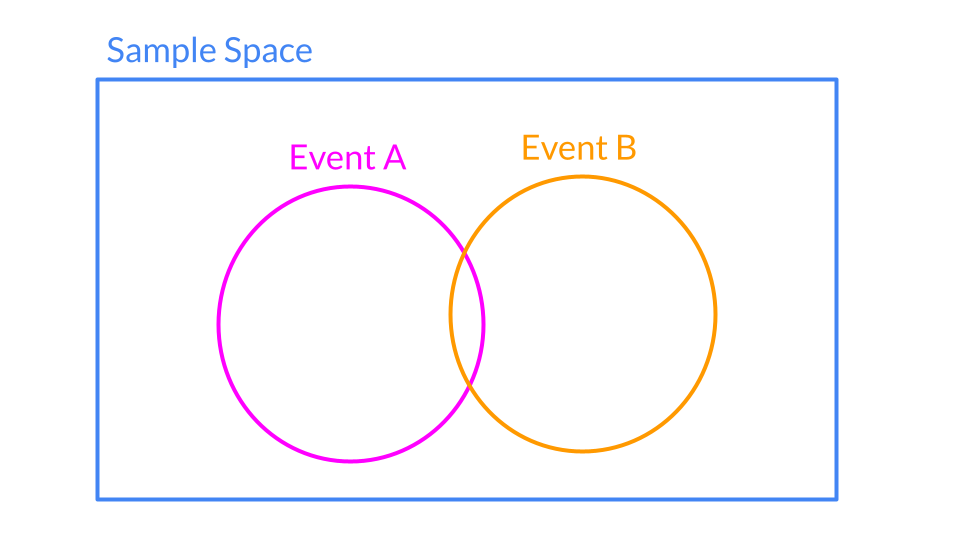
\includegraphics{graphics/ch2-venn-diagram-basic.png}

}

\end{figure}%

On the Venn diagram then, the overlap between circles represents their
intersection, the combined area of two (or more) circles represents
their union, and everything outside of a given circle represents the
complement of a set. This can be a fairly useful method for representing
sample spaces, and for visualizing the basic set operations that we use
to manipulate events inside the sample spaces. A word of caution: Venn
diagrams are useful tools, but they are not suitable as proofs
themselves. It is possible to convince yourself of false truths if the
wrong diagrams are used, and as a result, Venn diagrams should be
thought of as aids to understanding, rather than asa rigorous tool in
and of themselves.\footnote{This is a general principle in mathematics.
  Coming up with one example that makes something \emph{seem} true does
  not form an argument demonstrating that it \emph{is} true. Venn
  Diagrams should largely be thought of as specific examples of the
  underlying phenomena, which are great if you're a visual learner!}

\begin{figure}[H]

\caption{\label{fig-venn-diagram-union}\textbf{Union:} The union of
events A and B is shaded here in red. The union of two sets is all of
the contents of both sets, including the overlap between the two.}

\centering{

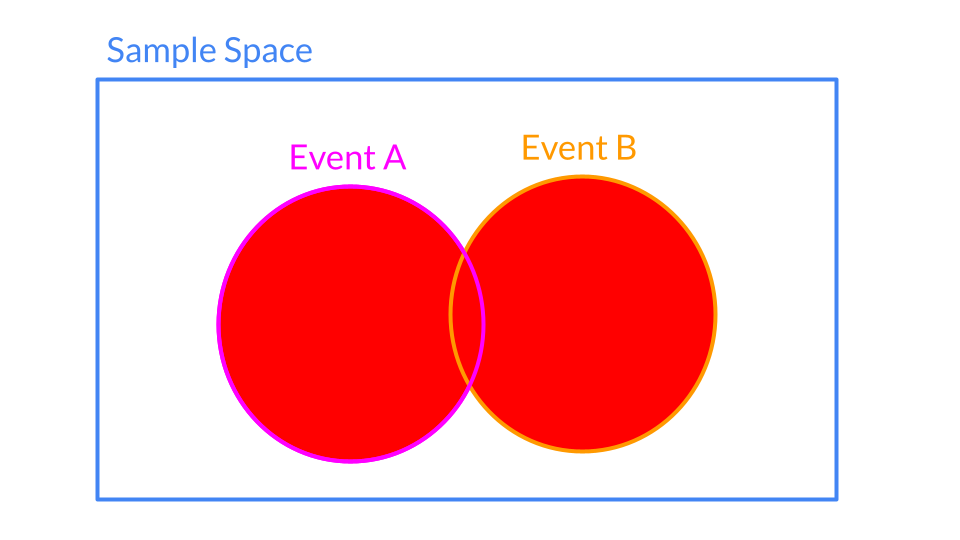
\includegraphics{graphics/ch2-venn-diagram-union.png}

}

\end{figure}%

\begin{figure}[H]

\caption{\label{fig-venn-diagram-intersection}\textbf{Intersection:} The
intersection of events A and B is shaded here in red. The intersection
of two sets is all of the content shared by both sets, given by the
overlapping area of the two circles.}

\centering{

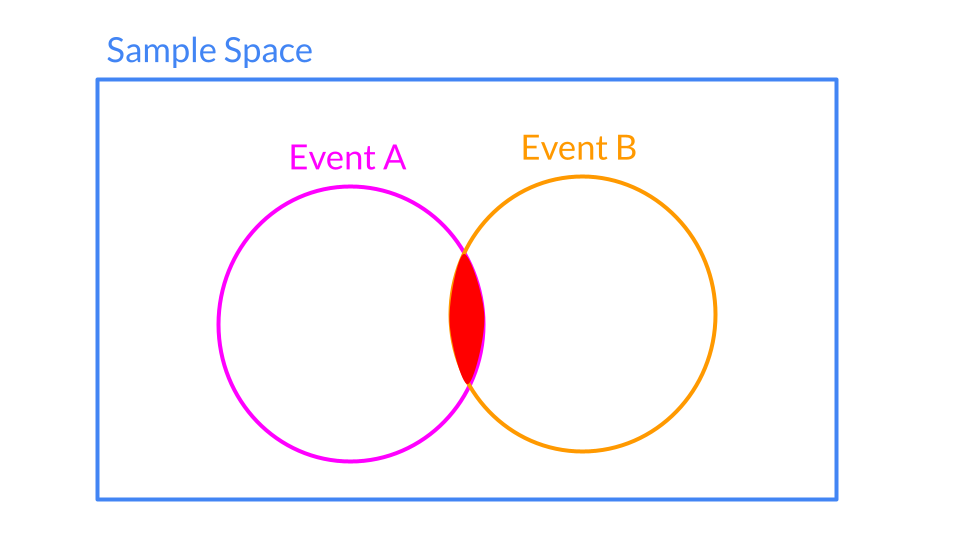
\includegraphics{graphics/ch2-venn-diagram-intersection.png}

}

\end{figure}%

\begin{figure}[H]

\caption{\label{fig-venn-diagram-complement}\textbf{Complement:} The
complement of event A is shaded here in red. The complement of a sets is
all of area inside of the sample space, not inside of the set. Here we
show the complement of Event A, though Event B would be similar.}

\centering{

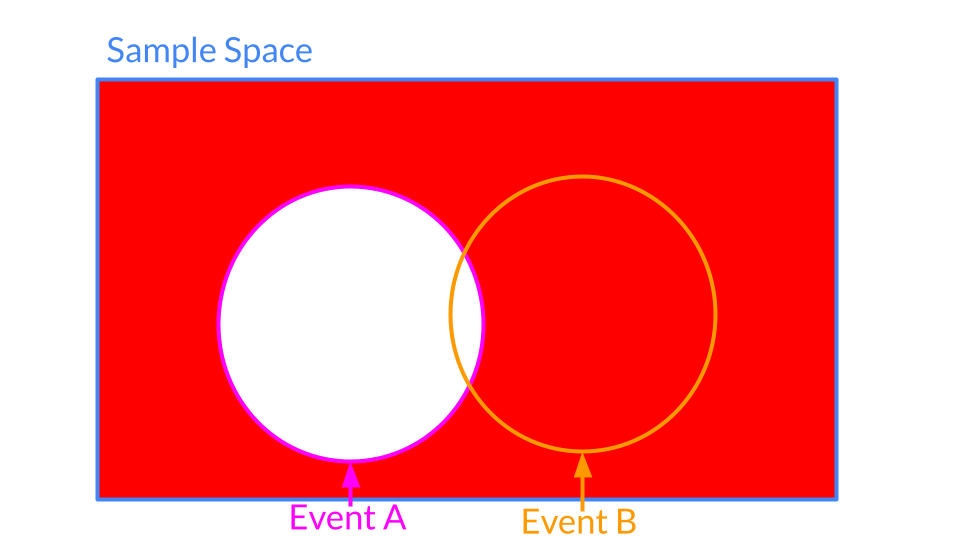
\includegraphics{graphics/ch2-venn-diagram-complement.png}

}

\end{figure}%

\newpage{}

\begin{example}[Venn Diagram with Defined
Events]\protect\hypertarget{exm-charles-and-sadie-vd}{}\label{exm-charles-and-sadie-vd}

Draw a Venn diagram representing the original game that Charles and
Sadie played. On the diagram draw the events corresponding to ``At least
one head \textbf{and} one tail are observed'', and ``Sadie won the
game''. Recall that three coins are tossed, and Sadie wins if at least
two of them show heads.

\begin{tcolorbox}[enhanced jigsaw, colback=white, breakable, rightrule=.15mm, leftrule=.75mm, toprule=.15mm, left=2mm, arc=.35mm, opacityback=0, bottomrule=.15mm]

\vspace{-3mm}\textbf{Solution}\vspace{3mm}

The sample space contains the eight possible options. Only
\((\text{T}, \text{T}, \text{T})\) does not belong to at least one of
the events. Both events share \((\text{H},\text{H},\text{T})\),
\((\text{H},\text{T},\text{H})\), and \((\text{T},\text{H},\text{H})\).

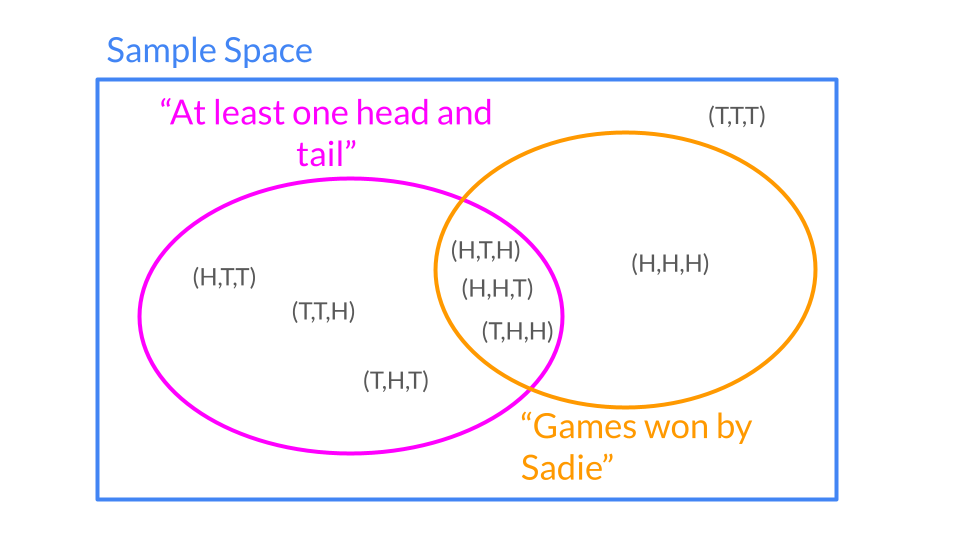
\includegraphics{graphics/ch2-venn-diagram-example.png}

\end{tcolorbox}

\end{example}

Sample spaces, events, and the manipulation of these quantities forms a
critical component of understanding probability models. In particular,
they describe the complete set of occurrences in a statistical
experiment that we could be interested in assigning probability values
to. To formalize a probability model, however, we also need some rule
for assigning probability values.

\section*{Exercises}\label{exercises}
\addcontentsline{toc}{section}{Exercises}

\markright{Exercises}

\begin{exercise}[]\protect\hypertarget{exr-2.1}{}\label{exr-2.1}

For each of the following experiments, describe the relevant sample
space and identify one possible event of interest.

\begin{enumerate}
\def\labelenumi{\alph{enumi}.}
\tightlist
\item
  The quality control inspection of smartphone screens from a
  manufacturing process.
\item
  Monitoring the ongoing structural integrity of a newly built bridge.
\item
  A clinical trial studying the effectiveness of a new drug.
\item
  Epidemiological monitoring of a disease outbreak.
\item
  Dealing a hand of black jack.
\item
  Observing the launch conditions for a rocket launch.
\item
  Debugging in software development.
\item
  Playing the lottery.
\end{enumerate}

\end{exercise}

\begin{exercise}[]\protect\hypertarget{exr-2.2}{}\label{exr-2.2}

A card is drawn at random from an ordinary deck of \(52\) playing cards.
Let \(A\) be the event that a king is drawn, and \(B\) the event that a
club is drawn. In words, describe the following events.

\begin{enumerate}
\def\labelenumi{\alph{enumi}.}
\tightlist
\item
  \(A\cup B\);
\item
  \(A \cap B\);
\item
  \(A\cup B^C\);
\item
  \(A^C\cup B^C\);
\item
  \((A\cap B)\cup(A\cap B^C)\).
\end{enumerate}

\end{exercise}

\begin{exercise}[]\protect\hypertarget{exr-2.3}{}\label{exr-2.3}

Suppose that \(\mathcal{S} = \{\phi, \lambda, \Delta, \mu\}\). List all
possible events from the corresponding experiment.

\end{exercise}

\begin{exercise}[]\protect\hypertarget{exr-2.4}{}\label{exr-2.4}

Suppose an experiment is run which generates realizations from positive
integers. Take \(A\) to be the event \(\{1, 5, 31, 56, 101\}\),
\(B = \{22, 56, 5, 103, 87\}\), \(C = \{41, 13, 7, 101, 48\}\), and
\(D\) to be the event that the number is odd. Identify (write down or
describe) each of the following events.

\begin{enumerate}
\def\labelenumi{\alph{enumi}.}
\tightlist
\item
  \(D^C\)
\item
  \(A\cap B\)
\item
  \(C \cup A\)
\item
  \(C \cap D\)
\item
  \((A\cup B)\cup (C\cup D)\)
\item
  \(A\cap D^C\)
\end{enumerate}

\end{exercise}

\begin{exercise}[]\protect\hypertarget{exr-2.5}{}\label{exr-2.5}

Suppose that a \(20\) sided die is rolled. The events of interest are:
\(A\) the outcome is a multiple of \(4\), and \(B\) the outcome is a
multiple of \(5\).

\begin{enumerate}
\def\labelenumi{\alph{enumi}.}
\tightlist
\item
  Draw a Venn Diagram representing the sample space and events.
\item
  Identify the event \(A \cup B\). What does this correspond to in
  words?
\item
  Identify the event \(A \cap B^C\). What does this correspond to in
  words?
\item
  How would you denote the event ``neither a multiple of \(4\) nor
  \(5\).'\,' using this notation?
\end{enumerate}

\end{exercise}

\begin{exercise}[]\protect\hypertarget{exr-2.6}{}\label{exr-2.6}

Suppose that two indistinguishable coins are flipped. The events of
interest are: \(A\) exactly two heads are seen, and \(B\) at least one
head is seen.

\begin{enumerate}
\def\labelenumi{\alph{enumi}.}
\tightlist
\item
  Draw a Venn Diagram representing the sample space and events.
\item
  Describe every possible outcome with respect to the identified events.
\item
  Give an event, in terms of the number of heads observed, which is
  equivalent to the sample space.
\end{enumerate}

\end{exercise}

\begin{exercise}[]\protect\hypertarget{exr-2.7}{}\label{exr-2.7}

A cinema has \(12\) screens, numbered \(1\) through \(12\). Before
opening, an employee checks to ensure that the projectors are correctly
calibrated.

Let \(A\) be the event that all the screens are correctly calibrated,
\(B\) be the event that the third screen is not correctly calibrated,
\(C\) be the event that exactly one bolt is not correctly calibrated,
and \(D\) be the event that \(5\) and \(8\) are correctly calibrated.

Which of the following pairs of events are disjoint?

\begin{enumerate}
\def\labelenumi{\alph{enumi}.}
\tightlist
\item
  \(A\) and \(B\).
\item
  \(B\) and \(D\).
\item
  \(C\) and \(D\).
\item
  \(B\) and \(C\).
\end{enumerate}

\end{exercise}

\chapter{The Core Concepts of
Probability}\label{the-core-concepts-of-probability}

\section{Assigning Probabilities (and The Equally Likely Outcome
Model)}\label{assigning-probabilities-and-the-equally-likely-outcome-model}

There are a plethora of ways to assign probabilities to different
events. At the most basic level any rule that maps from the space of
possible events to real numbers between \(0\) and \(1\) can be used as
rules for probability assignment. That is, probability assignment is
simply a set of rules which says ``for this event assign this
probability.''

\begin{example}[Coin Toss
Probabilities]\protect\hypertarget{exm-coin-toss}{}\label{exm-coin-toss}

Suppose that the fair coin used by Charles and Sadie is tossed one time.
Write down the probability assignments relating to this experiment.

\begin{tcolorbox}[enhanced jigsaw, colback=white, breakable, rightrule=.15mm, leftrule=.75mm, toprule=.15mm, left=2mm, arc=.35mm, opacityback=0, bottomrule=.15mm]

\vspace{-3mm}\textbf{Solution}\vspace{3mm}

In this case we have \(\mathcal{S} = \{\text{H},\text{T}\}\). Thus, the
possible events for which we need to assign probabilities are
\(\emptyset\), \(\{\text{H}\}\), \(\{\text{T}\}\), and
\(\{\text{H},\text{T}\} = \mathcal{S}\). For any probability model we
have \(P(\emptyset) = 0\) and \(P(\mathcal{S}) = 1\). When we say that a
coin is ``fair'' we are saying that \(P(\text{T}) = P(\text{H})\), and
since these are the only two possible outcomes in the sample space, we
must have that they each have probability \(0.5\).

\end{tcolorbox}

\end{example}

Not every assignment of probability values is going to be valid.
Suppose, for instance, that we have a six-sided die, each side labelled
with a number from one to six. If I told you that there was a
probability of \(0.5\) that it comes up \(1\), \(0.5\) that it comes up
\(2\), \(0.5\) that it comes up \(3\), \(0.5\) that it comes up \(4\),
\(0.5\) that it comes up \(5\), and \(0.5\) that it comes up \(6\), you
would probably call me a liar.\footnote{Or else conclude that I was
  mistaken and maybe should not be teaching probability.} If, as we have
previously seen, probabilities represent the long run proportion of time
that a particular event is observed, we cannot have \(6\) different
outcomes each occurring in half of all cases.

Beyond the requirements that we impose on what constitutes a ``valid''
probability rule, we have another concern: scalability. It is perfectly
acceptable to indicate that in an experiment with \(3\) outcomes, the
first has a probability of \(0.25\), the second of \(0.3\), and the
third of \(0.45\). What if the experiment has \(100\) possible outcomes?
Or \(1000\)? It quickly becomes apparent that enumerating the
probabilities of each event in the sample space is an efficient way of
assigning probabilities in practice. A core focus of our study of
probability will be finding techniques that allow us to efficiently
encode probability information into manageable objects. Once we have
done this we will be in a position where we can manipulate these
(comparatively) simple mathematical quantities in order to make
statements and conclusions about any of the events of interest, even if
they have never been explicitly outlined as having an assigned
probability.

While we will consider myriad methods for accomplishing these goals
throughout our study of probability, we begin with a very useful model
which simplifies probability assignment, without any added complexity,
and creates a solid foundation for us to explore the properties of
probability models. We start by considering \textbf{equally likely
outcomes.} As the name suggests, the probability model considering
equally likely outcomes assigns an equal probability to every possible
outcome of the experiment. This is a probability model that we are
already distinctly familiar with: flipping a coin, rolling a die, or
drawing a card are all examples of experiments which rely on the equally
likely outcomes framework.

\begin{remark}[Statisticians and Urn Models]
In statistics and probability courses and books you will often have
instructors or authors using fairly simple models to illustrate
probability concepts. There will often be questions relating to coin
tosses, and dice, and decks of cards, and everyone's favourite: urns. It
will very frequently be the case that a statistics question will state
that there is an urn with some combination of coloured balls within it,
from which you will be selecting some number either with or without
replacement. The frequency of these types of examples and questions
often feels disconnected from the refrain that ``uncertainty is all
around us'' and that ``statistics is relevant to every aspect of our
world!''\footnote{One of the most famous quotes from a statistician was
  a thought shared by John Tukey, stating ``The best thing about being a
  statistician is that you get to play in everyone's backyard.'' This is
  a common refrain, and one rooted in truth. Statistics is everywhere,
  across every field of human inquiry, and can help us make sense of
  everything from the trivial to the deeply important.} Why is it that
we seldom see questions or examples that are directly tied to these wide
spread applications of the lessons and techniques being taught?

In part these simple experiments are cleaner to handle than ``real
world'' situations. We can easily assume that a die is fair and that
takes care of any unsuspecting wrinkles that will necessarily come along
with the ``real world''. This is not dissimilar to working under the
assumption of frictionless surfaces in introductory physics, or assuming
that human beings are rational in economics. Another key point is that
most of us have deep familiarity with dice, and coins, and
cards.\footnote{This does not help to explain why we use urns so much,
  of course. When was the last time any of us drew a ball from an urn?}
The same is not going to be true of stories that are derived from
different use cases in the real world. A final important point, and this
will be something we see in depth in the coming chapters, is that from a
statistical point of view: there is no difference. Once we have the
tools to work with these quantities, we have the tools to work with any
of the quantities. This actually distinguishes the use of these types of
examples in statistics and probability from those for other subjects: at
no point is anything that we are learning incorrect, or overly simple -
we are just focusing on the raw probabilistic nature of the phenomenon.
As a result, we will continue to see these simple models in these notes.
I would encourage you, whenever possible, to hold a topic in mind that
matters more to you and start trying to draw the parallels between
rolling dice, and whatever it is that you may care about.

Why urns, specifically? Well, whether it be coin flipping or dice
rolling or card selection, we can model this equivalently using an urn
(with \(2\), \(6\), and \(52\) items, respectively). The urn becomes
more flexible to \emph{exactly} dictate what the probability of any
selection will be, which is a useful way of moving from equally likely
models (each ball is equally likely to be selected) to arbitrary models
(we can have however many identical balls in the urn as we would like).
\end{remark}

If we have an experiment with a sample space \(\mathcal{S}\) which has
\(|\mathcal{S}| = k\) total elements\footnote{Note that, when we have a
  set, using the absolute value symbols \(|\cdot|\) stands for the
  \textbf{cardinality} of the set. Cardinality is just a fancy way of
  saying the size or the number of elements that the set has in it.},
then each element of the sample space occurs with probability
\(\frac{1}{k}\). In the case of the coin toss example,
\(\mathcal{S} = \{\text{H}, \text{T}\}\), and so \(k=2\) and each
outcome occurs with probability \(\frac{1}{2}\). In the case of drawing
a card at random, there are \(52\) different outcomes, and so \(k=52\),
and the probability of drawing any particular card is \(\frac{1}{52}\).

It is critically important to recognize that the equal probability model
assigns equal likelihood to the possible outcomes of an experiment, not
the possible events of interest. It will not be the case that all events
have the same probability. To make this concrete, consider the events
\(A\) ``the ace of spades is drawn'' and \(B\) ``any spade is drawn''.
It is clear that \(B\) happens more frequently than \(A\), even though
we have said that this is an experiment with equally likely outcomes.
Remember: an outcome is an observation from a single experimental run,
an event is any collection of these possible outcomes.

A core goal is then bridging the gap between the probability of an
outcome\footnote{A quantity which in the equally likely outcome
  framework, we know exactly.} and the probability of an event. In order
to do so, we will next consider the rules of probability, introducing
properties that are required for valid probability assignments, and the
techniques for manipulating probabilities to calculate the probabilities
of quantities of interest.

\subsection{Using R for the Equally Likely Probability
Model}\label{using-r-for-the-equally-likely-probability-model}

In the previous chapter we saw how we can codify sample spaces and
events using vectors in R. In the introduction we actually saw how can
sample from a sample space using the equally likely outcome framework.
Specifically, an application of the \texttt{sample} function will draw a
set number of values from a sample space, giving each value an equal
probability to be drawn.\footnote{The \texttt{sample} function can also
  be used without equally likely events by specifying a vector of
  probabilities, however, this is a less common use case.}

\begin{Shaded}
\begin{Highlighting}[]
\CommentTok{\# Define the Sample Space of Rolling a 20 Sided Die}
\NormalTok{sample\_space }\OtherTok{\textless{}{-}} \DecValTok{1}\SpecialCharTok{:}\DecValTok{20}

\CommentTok{\# Recall that whenever we wish to perform an experiment in R with}
\CommentTok{\# randomness, we should call set.seed}
\FunctionTok{set.seed}\NormalTok{(}\DecValTok{31415}\NormalTok{)}

\CommentTok{\# The sample function takes three main parameters:}
\CommentTok{\#   x: the sample space}
\CommentTok{\#   size: the number of items to draw}
\CommentTok{\#   replace: a boolean representing whether the draws should be}
\CommentTok{\#            with replacement or not.}
\NormalTok{one\_roll }\OtherTok{\textless{}{-}} \FunctionTok{sample}\NormalTok{(}\AttributeTok{x =}\NormalTok{ sample\_space, }\AttributeTok{size =} \DecValTok{1}\NormalTok{)}
\NormalTok{ten\_rolls\_with\_replacement }\OtherTok{\textless{}{-}} \FunctionTok{sample}\NormalTok{(}\AttributeTok{x =}\NormalTok{ sample\_space, }
                                     \AttributeTok{size =} \DecValTok{10}\NormalTok{, }
                                     \AttributeTok{replace =} \ConstantTok{TRUE}\NormalTok{)}
\NormalTok{ten\_rolls\_without\_replacement }\OtherTok{\textless{}{-}} \FunctionTok{sample}\NormalTok{(}\AttributeTok{x =}\NormalTok{ sample\_space, }
                                        \AttributeTok{size =} \DecValTok{10}\NormalTok{, }
                                        \AttributeTok{replace =} \ConstantTok{FALSE}\NormalTok{)}

\NormalTok{one\_roll}
\NormalTok{ten\_rolls\_with\_replacement}
\NormalTok{ten\_rolls\_without\_replacement}
\DocumentationTok{\#\# [1] 2}
\DocumentationTok{\#\#  [1] 19 17 14  3  5 12  2 15  9  3}
\DocumentationTok{\#\#  [1] 18  8 16  9  7 20  2 19 10 13}
\end{Highlighting}
\end{Shaded}

\section{The Axioms of Probability}\label{the-axioms-of-probability}

We have previously seen that not every probability assignment can be
valid. For instance, assigning \(0.5\) probability to each outcome on a
die leads to a nonsensical scenario. With just a little imagination, we
can conjure equally nonsensical scenarios in other ways. For instance,
it would make very little sense to discuss the probability of an event
being a negative value. What would it mean for an event to occur in a
negative proportion of experimental runs? Alternatively, we can consider
two events that are nested in one another: say event \(A\) is that we
draw the ace of spades, and event \(B\) is that we draw any spade. Every
single time that \(A\) happens, we know that \(B\) also happens. But
there are ways that \(B\) can occur where \(A\) does not.\footnote{For
  instance, the Queen of spades being drawn.} If I told you the
probability of \(A\) was \(0.5\) and the probability of \(B\) was
\(0.2\), this would violate our base instincts. How can it be more
likely to draw the ace of spades than it would be to draw any spade at
all?\footnote{This is actually a scenario where our instincts may lead
  us awry in some situations. Consider the following from Kahneman and
  Tversky (1972): {Linda is 31 years old, single, outspoken, and very
  bright. She majored in philosophy. As a student, she was deeply
  concerned with issues of discrimination and social justice, and also
  participated in anti-nuclear demonstrations. Which is more probable?
  (a) Linda is a bank teller, or (b) Linda is a bank teller and is
  active in the feminist movement.} A majority of respondents rate (b)
  as being more probable, even though (a) is contained in (b).}

Often in mathematics when we have an intuitive set of rules\footnote{These
  rules, which we call ``properties'' are formally known as ``axioms''.}
that particular quantities must obey, we work to add formality through
defining properties of these concepts. To this end, we can define the
key properties that probabilities must obey in order to be well-defined,
valid probabilities. With three fairly basic properties, we can
completely specify what must be true in order for a set of probabilities
to be ``valid'', and to in turn match with our intuitions.

\begin{tcolorbox}[enhanced jigsaw, rightrule=.15mm, leftrule=.75mm, opacitybacktitle=0.6, title={The Axioms of Probability}, colframe=quarto-callout-tip-color-frame, opacityback=0, coltitle=black, breakable, toptitle=1mm, colbacktitle=quarto-callout-tip-color!10!white, bottomtitle=1mm, titlerule=0mm, arc=.35mm, colback=white, toprule=.15mm, left=2mm, bottomrule=.15mm]

\begin{enumerate}
\def\labelenumi{\arabic{enumi}.}
\tightlist
\item
  \textbf{Unitary:} Every valid set of probabilities must assign a
  probability of \(1\) to the full sample space. That is,
  \(P(\mathcal{S}) = 1\). This is an intuitive requirement as every time
  the experiment is run we observe an outcome in the sample space. As a
  result, in every experimental run the event \(\mathcal{S}\) occurs.
\item
  \textbf{Non-negative:} We require that every probability is
  non-negative. We can have probabilities of \(0\), but we can never
  have a probability less than zero. Again, this is
  sensible\footnotemark{} but is important to include in our
  formalization. Specifically, for every event \(E\), we must have
  \(P(E) \geq 0\).
\item
  \textbf{Additivity:} the final property requires slightly more parsing
  on first pass. Suppose that we define a sequence of events,
  \(E_1, E_2, E_3, \dots\) such that no two events have any overlap.
  That is, \(E_j \cap E_\ell = \emptyset\) for all \(\ell\neq j\). Then,
  the final property we require for probabilities is that
  \[P\left(\bigcup_i E_i\right) = \sum_i P(E_i).\] That is, the
  probability of the union of disjoint events is the summation of the
  probability of these events.
\end{enumerate}

\end{tcolorbox}

\footnotetext{What would it mean to have a negative probability? It is
perhaps a more interesting question than it seems at first glance. It is
a topic that has come up in some pretty strange places and, while it is
not presently sensible to call them ``probabilities'' in a traditional
sense, there are interesting results which follow.}

It is worth dwelling slightly on axiom 3. Consider the case of drawing a
card at random from a deck of \(52\) cards. Using the equally likely
outcome model for probability we know that the probability that any card
is drawn is given by \(\frac{1}{52}\). If I were to ask ``what is the
probability you draw that ace of spades?'' under this model you can
respond, immediately, with \(\frac{1}{52}\). Now, if I were to ask
``what is the probability that you draw the ace of spades or the two of
spades?'' then intuitively you likely figure that this will be
\(\frac{2}{52}\). Note that the event \(E_1\), ``draw the ace of
spades'' and the event \(E_2\) ``draw the two of spades'', are disjoint
events. Moreover, recall that the union is the ``or'' and so
\(E_1\cup E_2\) is the same as \(E_1\) or \(E_2\). Taken together then,
\[P(E_1\cup E_2) = P(E_1) + P(E_2).\] The axiom of additivity simply
extends this intuition to an arbitrary number of events.

\begin{example}[Basic
Additivity]\protect\hypertarget{exm-additivity}{}\label{exm-additivity}

Still unsure of how best to go about using cards to replace their coin
game, Charles and Sadie are considering various different events and
trying to understand their probabilistic behaviour. They take \(S\),
\(C\), \(H\), and \(D\) to be the events that a spade, club, heart, or
diamond are drawn from a standard deck of cards, respectively. Further,
they take \(C_j\) to be the event that a card with denomination \(j\) is
drawn (\(j\) ranging from ace with \(1\) through King with \(13\)). If
they consider the union of any two (or more) of these events when can
they leverage properties of additivity? When can't they?

\begin{tcolorbox}[enhanced jigsaw, colback=white, breakable, rightrule=.15mm, leftrule=.75mm, toprule=.15mm, left=2mm, arc=.35mm, opacityback=0, bottomrule=.15mm]

\vspace{-3mm}\textbf{Solution}\vspace{3mm}

In order to use the properties of additivity it is required that the two
events are disjoint. Note that taking any two (or more) of \(S\), \(C\),
\(H\), and \(D\) will lead to disjoint events. There is no way to draw a
card which has two suits on it at once. Similarly, taking any two (or
more) of \(C_j\) will lead to disjoint events. However, mixing any of
the suited events (\(S\), \(C\), \(H\), and \(D\)) with any \(C_j\) will
not be disjoint.

Consider \(S\cap C_1\). The ace of spades is in \(S\) since it is a
spade and it is in \(C_1\) since it is an ace. As a result,
\(S\cap C_1 = \{\text{Ace of Spades}\}\). Because of this we are not
able to say that \(P(A \cup C_1) = P(A) + P(C_1)\). However, we can say
that \[P(S\cup C\cup H\cup D) = P(S) + P(C) + P(H) + P(D),\] and could
do the same with any subset of these sets. Similarly, we can take
\[P\left(\bigcup_{j=1}^{13} C_j\right) = \sum_{j=1}^{13} P(C_j),\] or
any of the subsets there.

\end{tcolorbox}

\end{example}

These three axioms fully define valid probabilities. Any mechanism that
assigns probability values to events which conforms to these rules will
assign valid probabilities. While it may seem counterintuitive that such
basic rules fully define our notion of a probability, these rules
readily give rise to many other properties that are indispensible when
working with probabilities.

\section{Secondary Properties of
Probabilities}\label{secondary-properties-of-probabilities}

Using the previously indicated axioms of probability we are able to
derive many useful \textbf{secondary properties}. These properties will
frequently be used to actually compute different probabilities, and are
helpful to become familiar with. All of the following properties follow
directly from the axioms, though, some are more clear than others. For
the following we take \(E\) and \(E_1,E_2,E_3,\dots\) to be arbitrary
events on some well defined sample space.

\begin{enumerate}
\def\labelenumi{\arabic{enumi}.}
\tightlist
\item
  \(P(E^C) = 1-P(E)\), and equivalently, \(P(E) = 1 - P(E^C)\).
\item
  \(P(\emptyset) = 0\).
\item
  \(P(E_1 \cup E_2) = P(E_1) + P(E_2) - P(E_1\cap E_2)\).
\item
  \[P(E_1 \cup E_2 \cup E_3) = P(E_1) + P(E_2) + P(E_3) - P(E_1\cap E_2) - P(E_1 \cap E_3) - P(E_2 \cap E_3) + P(E_1 \cap E_2 \cap E_3).\]
\item
  If \(E_1 \subset E_2\) then \(P(E_1) \leq P(E_2)\).
\end{enumerate}

\begin{tcolorbox}[enhanced jigsaw, rightrule=.15mm, leftrule=.75mm, opacitybacktitle=0.6, title={Proofs of the Secondary Properties of Probability}, colframe=quarto-callout-warning-color-frame, opacityback=0, coltitle=black, breakable, toptitle=1mm, colbacktitle=quarto-callout-warning-color!10!white, bottomtitle=1mm, titlerule=0mm, arc=.35mm, colback=white, toprule=.15mm, left=2mm, bottomrule=.15mm]

It may be instructive to see how these properties are derived. Doing so
generates added familiarity with manipulating probability expressions
and helps to encourage deeper understanding.

\begin{enumerate}
\def\labelenumi{\arabic{enumi}.}
\item
  Note that, for any event \(E\), by definition we have
  \(E \cup E^C = \mathcal{S}\) and \(E \cap E^C = \emptyset\). As a
  result, we can apply \textbf{additivity} to the sets \(E\) and \(E^C\)
  giving \(P(E \cup E^C) = P(E) + P(E^C)\). However, since
  \(E\cup E^C = \mathcal{S}\), then we know that
  \(P(E \cup E^C) = P(\mathcal{S}) = 1\) by the \textbf{unitary}
  property. Taken together this tells us that \(1 = P(E) + P(E^C)\), and
  rearranging gives \(P(E^C) = 1 - P(E)\), or \(P(E) = 1 - P(E^C)\), as
  required.
\item
  We know that \(\mathcal{S}^C = \emptyset\). Using secondary property
  (1), \(P(E) = 1 - P(E^C)\). Taking \(E = \emptyset\) gives
  \(P(\emptyset) = 1 - P(\mathcal{S}) = 1 - 1 = 0\), by the
  \textbf{unitary} property.
\item
  Here note that \(E_1 \cup E_2\) can be written as \(E_1 \cup E_2'\)
  where \(E_2' = E_2\cap E_1^C\). That is, \(E_2'\) contains the
  outcomes from \(E_2\) which were not shared by \(E_1\). Then
  \(E_1 \cap E_2' = \emptyset\) so we can write
  \(P(E_1 \cup E_2) = P(E_1 \cup E_2') = P(E_1) + P(E_2')\), by
  \textbf{additivity}. Now, if we define \(E_2^* = E_2\cap E_1\) then
  \(E_2 = E_2' \cup E_2^*\), and \(E_2'\cap E_2^* = \emptyset\). Thus,
  \(P(E_2) = P(E_2'\cup E_2^*) = P(E_2') + P(E_2^*)\). Rearranging this
  gives \(P(E_2') = P(E_2) - P(E_2^*)\), and we know that
  \(P(E_2^*) = P(E_1 \cap E_2)\). Thus, plugging into what we found
  before we get
  \[P(E_1 \cup E_2) = P(E_1) + P(E_2') = P(E_1) + P(E_2) - P(E_1 \cap E_2).\]
\item
  This follows exactly from the argument for (3). To see, first consider
  \(E_2 \cup E_3\) to be an event itself, say \(E_4\). Then we can apply
  the above result to \(E_1 \cup E_4\). And then we need only repeat the
  process for the remaining terms.
\item
  We can rewrite \(E_2\) as \(E_1 \cup (E_2 \cap E_1^C)\). These two
  sets are disjoint, since the one is \(E_1\) and the other must contain
  only elements in \(E_1^C\). Then,
  \(P(E_2) = P(E_1) + P(E_2 \cap E_1^C)\) by \textbf{additivity}. Then,
  through the \textbf{non-negative} property we know that
  \(P(E_2 \cap E_1^C) \geq 0\), and so rearranging we have
  \(P(E_1) = P(E_2) - P(E_2\cap E_1^C) \leq P(E_2)\).
\end{enumerate}

\end{tcolorbox}

These properties are immensely useful when computing probabilities. In
fact, these secondary properties will be used with more frequency than
the basic axioms when manipulating probabilities in practice. It is
worth building comfort with these properties, early and often, as they
will assist in manipulating all probability expressions in the future.

While these properties hold in general for all probability models, it is
instructive to focus on the equal probability model to begin building
familiarity with probability. These properties allow us to take events
-- whether compound or simple -- and combine, rewrite, and manipulate
expressions to assist in the handling of the computations. Eventually,
however, we require the ability to assign numerical values to these
probabilities.

Consider a simple event, \(A\). Recall that a simple event is defined as
a possible outcome of an experiment, and so in this case, \(A\)
corresponds directly to an event that may be observed. If our sample
space is \(k\) elements large, then \(P(A) = \frac{1}{k}\) in this
framework. For instance, if \(A\) is the event that a two is rolled on a
six-sided fair die, then \(P(A) = \frac{1}{6}\).

Now, suppose that a compound event is defined, \(B\). By definition, a
compound event can be expressed as a set of possible outcomes from the
experiment. Suppose that we enumerate these possible events as
\(b_1, b_2, \dots, b_\ell\). Then we know that \(B\) occurs if any of
\(b_1,b_2,\dots,b_\ell\) occur. Each \(b_j\) are elements of the sample
space and correspond to possible outcomes of the experiment. As a
result, we know that \(P(b_j) = \frac{1}{k}\), based on the equal
probability assumption. Now, if we take any two distinct events, say
\(b_i\) and \(b_j\), we know that they must be disjoint:
\(b_i \cap b_j = \emptyset\). This is because in an experiment run only
one outcome can occur. Moreover, we can say that
\(B = b_1 \cup b_2 \cup\cdots\cup b_\ell\).

Using the axioms of probability outlined above we therefore know that
\(P(B) = \sum_{j=1}^\ell P(b_j) = \sum_{j=1}^\ell \frac{1}{k} = \frac{\ell}{k}\).
This holds in general for any compound event in this setting. If we take
\(B\) to be the event that an even number is rolled on a six-sided die,
then we would have \(b_1\) is the event that a two is rolled, \(b_2\) is
the event that a four is rolled, and \(b_3\) is the event that a six is
rolled. There are three such events, and so the probability that an even
number is rolled must be \(\frac{3}{6} = 0.5\), which matches our
intuition.

If we consider what this process is doing at its core, we can reframe
the calculation as counting up the number of ways that event can happen
and dividing by the total number of events. In our previous discussion,
there were \(\ell\) ways of \(B\) occurring, a total of \(k\) outcomes,
and so the probability becomes \(\frac{\ell}{k}\). In the equal
probability model, this will always be the case. The probability of any
event \(A\) occurring is given by \[P(A) = \frac{N_A}{k},\] where
\(N_A\) is the number of unique ways that \(A\) can occur. In other
words, \(N_A\) is the size of the set \(A\), \(|A|\).

As a result of this, computing probabilities largely relies on the
counting of possible outcomes corresponding to different events. If we
can determine \(N_A = |A|\), and the count of the total number of
occurrences, \(k\), then we can determine the probability of \(A\). This
study of counting is known as \textbf{combinatorics}, and it is where we
will turn our attention next.

\begin{example}[Unmatched Six-Sided
Dice]\protect\hypertarget{exm-complement-trick}{}\label{exm-complement-trick}

Charles and Sadie, not all together content with the progress through
decks of cards, are considering games with dice. Suppose that they have
two, fair, six-sided dice. They are interested in the probability that
the two dice show different numbers when they are rolled. What is this
probability?

\begin{tcolorbox}[enhanced jigsaw, colback=white, breakable, rightrule=.15mm, leftrule=.75mm, toprule=.15mm, left=2mm, arc=.35mm, opacityback=0, bottomrule=.15mm]

\vspace{-3mm}\textbf{Solution}\vspace{3mm}

Here, the key is to realize that the probability is easier to solve when
considering the complement rather than the event itself. Notably,
rolling two, fair, six-sided dice gives a total of \(36\) possible
outcomes. Of these, exactly \(6\) have equal numbers showing on both
dice. Thus, the probability that the two dice show the \textbf{same}
number is going to be \(\frac{6}{36} = \frac{1}{6}\). Then, using the
fact that \(P(E) = 1 - P(E^C)\), and that taking \(E\) to refer to the
event where the two dice show different numbers, then \(E^C\) refers to
the event that the two dice show the \emph{same} number. As a result,
the probability that we want is
\(P(E) = 1 - \frac{1}{6} = \frac{5}{6}\).

\end{tcolorbox}

\end{example}

\begin{example}[Unmatched Arbitrary
Dice]\protect\hypertarget{exm-complement-trick-two}{}\label{exm-complement-trick-two}

Charles and Sadie, working from their intrigue about dice, have decided
that instead of using two six-sided dice, they wish to take two dice of
possibly different sizes. Suppose that the first die has \(d_1\) sides
and the second has \(d_2\) sides, and that both dice are otherwise fair.
They are interested in the probability that the two dice show different
numbers when they are rolled. What is this probability?

\begin{tcolorbox}[enhanced jigsaw, colback=white, breakable, rightrule=.15mm, leftrule=.75mm, toprule=.15mm, left=2mm, arc=.35mm, opacityback=0, bottomrule=.15mm]

\vspace{-3mm}\textbf{Solution}\vspace{3mm}

This problem is conceptually no different from
Example~\ref{exm-complement-trick}. There will be a total of
\(d_1\times d_2\) possible combinations of the two dice to be
rolled.\footnotemark{} Of these, the dice will match in
\(\min\{d_1, d_2\}\) events.\footnotemark{} Then, with the same
complement trick discussed above, we get
\[P(E) = 1 - P(E^C) = 1 - \frac{\min\{d_1,d_2\}}{d_1\times d_2}.\]

\end{tcolorbox}

\footnotetext{Note: if this is not yet clear to you, that's okay! In the
very next section we begin to discuss how to count the possible
combinations in these types of scenarios.}

\footnotetext{Suppose that \(d_1 = 2\) and \(d_2 = 4\). Then here, the
dice can match when they show either \(1\) or \(2\), but if the second
die shows \(3\) or \(4\) there is no possibility of having a match at
all.}

\end{example}

\section{Combinatorics}\label{combinatorics}

\subsection{The Product Rule}\label{the-product-rule}

Fundamentally, counting is a matter of assessing the size of a
collection of items. Sometimes, this is very straightforward. If you
want to count the number of students in a classroom, you start at \(1\)
and enumerate upwards through the integers. To count the number of days
until the next Holiday, you do the same thing. If you really need to
sleep, perhaps you will count imaginary sleep until you drift off. There
is not much to this type of counting, and it is certainly deeply
familiar to you all. However, it is also quite limited in its utility.

Imagine that you are interested in determining how many possible ways
there are of arranging a deck of \(52\) cards. You could of course
arrange them in a particular order, then count each of those. That would
take a tremendous amount of time, so perhaps instead of using an actual
deck you just write down the combinations. Still, each combination is
going to be \(52\) cards long, and keeping track of that all will be a
tremendous challenge. This seems like an approachable question, and yet,
it illustrates how complicated (and large) these types of ``counting''
problems can become very quickly.

Fortunately for us there are some strategies for simplifying these
problems down, some of which you are likely already familiar with. Think
about trying to form an outfit where you have \(4\) different sweaters,
\(3\) pairs of pants, and \(2\) options for your shoes. Suppose that any
combination of these will work well. How many total outfits are there?
Well, if you have already picked your sweater and pants, then there are
going to be \(2\) different outfits using these: one with each of the
pairs of shoes. This is true for each possible sweater-pant combination,
and so we can count \(2\) for each one these. In other words, to get the
total number of outfits we multiply the number of sweater-pant
combinations by the number of shoe options. The same rationale can be
applied to count the total number of sweater-pant combinations. For each
sweater, there are \(3\) pairs of possible pants, and so to get the
total number we can take \(3\) for each possible sweater, or in other
words, \(3\times 4\). Taken together then we have
\(4\times 3\times 2 = 24\) total possible outfits.

Another way of framing this is that we have to make three sequential
decisions: which of the \(4\) sweaters, which of the \(3\) pants, and
which of the \(2\) shoes are to be worn? When we do this we multiply
through the number of alternatives at each decision point to get the
total number of combinations. This is known as the \textbf{product rule
for counting}.

\begin{definition}[Product Rule for
Counting]\protect\hypertarget{def-product-rule-count}{}\label{def-product-rule-count}

The product rule for counting states that, when there are a sequence of
\(k\) decisions to be made, and for each decision \(j=1,\dots,k\), there
are \(n_j\) options, then the total number of combinations will be
\[N = n_1\times n_2\times\cdots\times n_k.\]

\end{definition}

\begin{example}[Counting Coffee
Orders]\protect\hypertarget{exm-counting-coffee-orders}{}\label{exm-counting-coffee-orders}

When Charles and Sadie are out for coffee, Sadie enjoys ordering the
same thing each time: a black coffee and vegan chocolate chip cookie.
Charles, on the other hand, has decided to work through the entire menu
of the local coffee shop, each day ordering a drink, with one add-in,
and a snack. If there are \(10\) different drinks, \(8\) possible
add-ins, and \(12\) different snacks, how many trips to the coffee shop
will it take until Charles has tried it all?

\begin{tcolorbox}[enhanced jigsaw, colback=white, breakable, rightrule=.15mm, leftrule=.75mm, toprule=.15mm, left=2mm, arc=.35mm, opacityback=0, bottomrule=.15mm]

\vspace{-3mm}\textbf{Solution}\vspace{3mm}

This necessitates an application of the product rule for counting.
Specifically, we can view this as three sequential decisions, where the
first decision is which drink (with \(n_1 = 10\)), the second decision
is which add-in (with \(n_2 = 8\)), and the third decision is which
snack (with \(n_3 = 12\)). Taking the product gives the total number of
combinations as \(10\times 8\times 12 = 960\). As a result, it will take
\(960\) visits (assuming that nothing on the menu changes!) to try all
combinations.

\end{tcolorbox}

\end{example}

\begin{example}[Sequence of Dice
Rolls]\protect\hypertarget{exm-rolling-sequence-of-dice}{}\label{exm-rolling-sequence-of-dice}

Charles and Sadie have been enjoying playing with dice, but they lost
one of the two they had. As a result, they are trying to come up with
games revolving around rolling a single die. They decide to try a game
called ``six is lava'', where they roll a single six-sided die \(10\)
times in a row. If they get \(1\) or more sixes, they lose the game.
They are not sure if \(10\) is the correct number of rolls to use. What
is the probability that they lose on any given set of \(10\) rolls of
the die in this game?

\begin{tcolorbox}[enhanced jigsaw, colback=white, breakable, rightrule=.15mm, leftrule=.75mm, toprule=.15mm, left=2mm, arc=.35mm, opacityback=0, bottomrule=.15mm]

\vspace{-3mm}\textbf{Solution}\vspace{3mm}

Once again this is a scenario where using the complement simplifies the
problem. If we asked ``what is the probability that no 6's are rolled,
on \(10\) rolls of the die'' then we can count the number of
possibilities through an application of the product rule. In particular,
there are going to be \(5\) options which are not \(6\) at each possible
step. We can view this as have \(n_1 = n_2 = \cdots = n_{10} = 5\).
Thus, the total number of ways of rolling \textbf{no} sixes is
\(5\times5\times5\times\cdots\times5 = 5^{10}\).

Essentially the same process can be used to count the total number of
possible rolls, replacing \(5\) with \(6\) to get the denominator. This
means that there are \(6^{10}\) total sequences of \(10\) rolls, and
\(5^{10}\) which contain no sixes. As a result, taking \(E\) to
represent the probability that we observe no sixes on \(10\) rolls of
the die, we would get \[P(E) = \frac{5^{10}}{6^{10}}.\] The question
asks for \(E^C\) and so we take
\[P(E^C) = 1 - P(E) = 1 - \left(\frac{5}{6}\right)^{10}.\] This is
approximately 0.8385.

Note that if instead of \(10\) flips they had \(n\) flips, the
probability would be \(1 - \left(5/6\right)^n\). We can plot this over
various values of \(n\), to see how the number of flips impacts this
probability. The probability of \(0.5\) is marked and we can see that
taking \(4\) tosses gives an ever so slightly greater than \(0.5\)
probability of losing (0.5177).

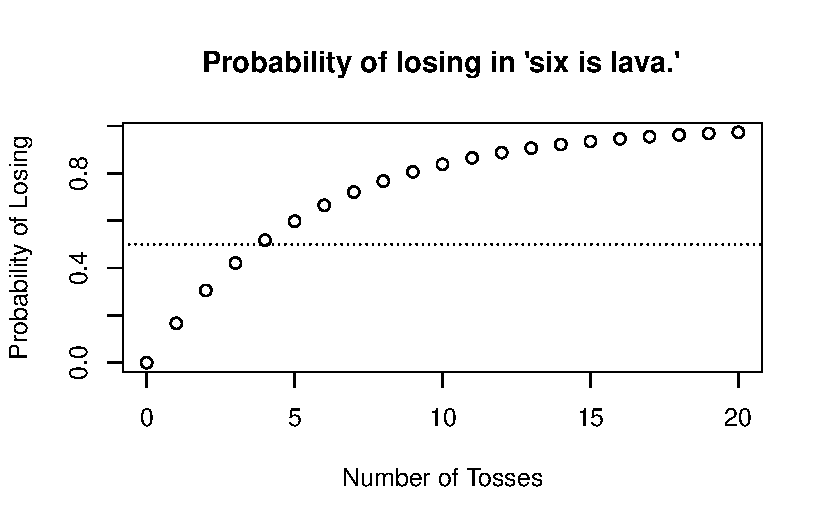
\includegraphics{notes/chapter3_files/figure-pdf/unnamed-chunk-2-1.pdf}

\end{tcolorbox}

\end{example}

\subsection{Tree Diagrams}\label{tree-diagrams}

Sometimes it is helpful to express counting rules graphically. To do so
we rely on tree diagrams.

\begin{definition}[Tree
Diagram]\protect\hypertarget{def-tree-diagram}{}\label{def-tree-diagram}

A tree diagram is a graphical representation for the product rule of
counting. Specifically, a tree diagram puts each of the decisions in
sequence, and draws a branch for each separate option, starting from the
branches drawn at the previous decision step.

\end{definition}

To draw a tree diagram, you start with the first choice, drawing one
branch for each of the \(n_1\) alternatives, labelling each. Then, at
the second choice, you do the same process at the end of each of the
branches you drew for choice \(1\), this time drawing \(n_2\) branches
there (so you will have just drawn \(n_1\times n_2\) branches). Then for
each of those you draw the \(n_3\) further branches, and so on and so
forth until the end.

If you want to know the total number of choices, you simply count the
end points at the very end of the diagram. Each branch corresponds to a
single option. To determine which combination of choices it corresponds
to, you simply read off the branch labels at each branch you take. If
you want to know how many possible combinations come with certain
options selected, you can look at only those branches which are
downstream from the choices that you care about.

\begin{figure}[H]

\caption{\label{fig-tree-diagram-general}A generic tree diagram. Here
the first choice has three different options and the second choice has
two. We can see the six total combinations, labelled on the right of the
diagram, and can trace the choices required to get there.}

\centering{

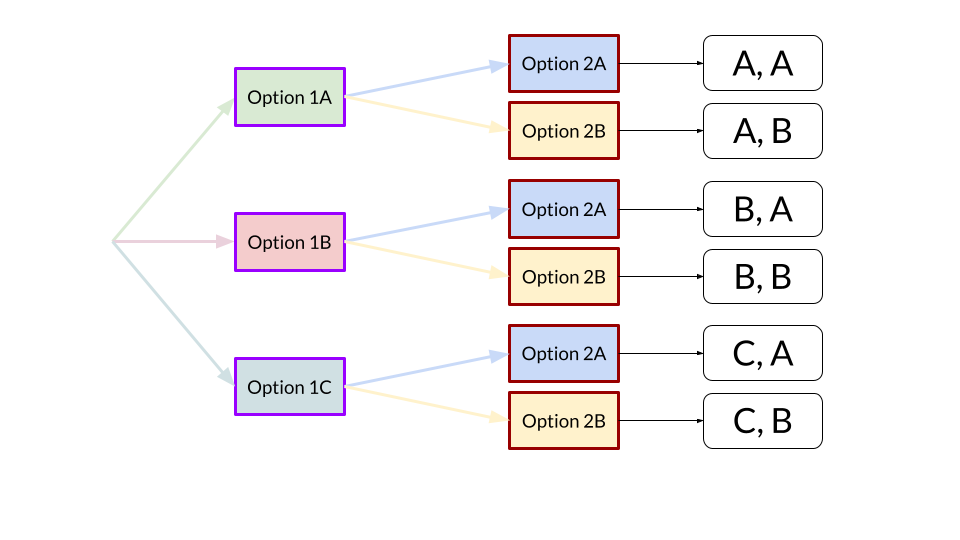
\includegraphics{graphics/ch3-tree-diagram-generic.png}

}

\end{figure}%

While tree diagrams can be quite useful for visualizing a problem, they
often grow to be overly complex. As a result, we need to fall back on
the numerical representation afforded to us through the product rule for
counting. Counting problems, in general, can very quickly become
tremendously large and complex. For this reason, we have several tools
to assist us in reducing this complexity based on common types of
problems that we would like to count.

\subsection{The Factorial}\label{the-factorial}

The first useful tool for simplifying these problems is the
\textbf{factorial}. The factorial of an integer, denoted by \(x!\) is
given by the product of all integers from \(x\) to \(1\).\footnote{Factorials
  are exciting because they always look like they are shouting!} That
is, \[x! = x(x-1)(x-2)\cdots(2)(1).\] If we consider the product rule
for counting then note that if \(n_1=1\), \(n_2=2\), \ldots{} ,
\(n_k = k\), then the total number of options is
\(k\times(k-1)\times\cdots\times 1 = k!\). The most common reason that
this comes up is when we want to order a collection of items. Suppose
that you have \(10\) books that you want to place on a shelf. You can
view this as making \(10\) sequential decisions: what book goes first,
second, third, and so on. There are \(10\) options for the first book,
then \(9\) for the second (any except for the first one), and then \(8\)
for the third (any except for the first \(2\)). This continues down to
the last book, and so we conclude that there are
\(10\times9\times8\times\cdots\times1 = 10!\) ways of arranging these
books.

\begin{example}[Seating in a (Full) Coffee
Shop]\protect\hypertarget{exm-factorial}{}\label{exm-factorial}

One day Charles and Sadie walk into the coffee shop and find that it is
completely full. There are ten seats and ten people sitting in them.
They are disappointed that they do not have room to sit themselves,
however, they are never ones to pass up an interesting probability
question.

\begin{enumerate}
\def\labelenumi{\alph{enumi}.}
\tightlist
\item
  How many different ways could these ten people have sat in these ten
  seats?
\item
  If there are ten drinks that have been made, and one is to be passed
  out to each seat, how many different ways can these ten people sit in
  these ten seats, with each of these ten drinks?
\item
  Alongside the ten drinks, there are ten snacks to be served up as
  well. How many different ways can these ten people sit in these ten
  seats, with each of these ten drinks, and each of these ten snacks?
\end{enumerate}

\begin{tcolorbox}[enhanced jigsaw, colback=white, breakable, rightrule=.15mm, leftrule=.75mm, toprule=.15mm, left=2mm, arc=.35mm, opacityback=0, bottomrule=.15mm]

\vspace{-3mm}\textbf{Solution}\vspace{3mm}

\begin{enumerate}
\def\labelenumi{\alph{enumi}.}
\item
  Here, we can think about lining up the ten seats in a row, each number
  \(1\) through \(10\). Then, we want to place one patron into each of
  the seats. This is no different from ordering \(10\) books, and so the
  total is \(10!\) which is \(3,628,800\).
\item
  Note that we still have to make the seat choices from part (a), so
  there are \(10!\) ways of getting the \(10\) people sat in the \(10\)
  chairs. Once there, we can think of handing out the drinks to each of
  the numbered combinations of person-chair. This is no different from
  passing out the people as well, giving \(10!\) ways of doing this. We
  use the product rule to combine these two choices, with
  \(10!\times 10!\) total combinations of people-chair-drink. This is
  \(13,168,189,440,000\).
\item
  Extending the same logic before, there are \(10!\times 10!\) ways of
  getting each person sat in a chair with a drink. Then, there will be
  an additional \(10!\) ways of passing out the snacks to these people.
  Taken together this gives \(10!\times 10!\times 10!\) which is
  \(47,784,725,839,872,000,000\).\footnotemark{}
\end{enumerate}

\end{tcolorbox}

\footnotetext{It is somewhat interesting to note how large these values
get relatively quickly. This is a comparatively small question: only
\(10\) people with \(10\) drinks and \(10\) snacks. If you consider any
counting problem with a larger number of items, these problems quickly
grow to be intensely complex. For instance, a count of my main home book
collection reveals \(376\) of them. To order these would give \(376!\)
possible orderings. In decimal representation this is
\[4.992244775852435618292576458782762114148884082811840265632\dots\times10^{806}.\]
This is an \(807\) digit long number. This is an incomprehensibly large
number. This number is \(8×10^{726}\) \textbf{times larger than} the
number of atoms in the universe. That is, if every atom in the universe
were given some arrangements of books to hold onto, they would need to
hold \(8×10^{726}\) of them in order for all of the arrangements to be
held. I point this out because combinatorics \emph{explodes} in this
way. Even simple problems grow out of hand very, very quickly. This is
where comfort with the algebraic tools is required, rather than a
reliance on intuition. There is simply no way to have intuition
regarding the scope of these numbers, at least, not without a lot of
practice.}

\end{example}

\begin{remark}[0!]
Depending on how factorials are thought of, some trouble can come up
around a quantity like \(0!\). On one hand, if we view factorials as
multiplying each number between \(n\) and \(1\) together then
\(0! = 0\times 1\) and we get \(0! = 0\). On the other hand, if we view
factorials as counting the number of ways which we can order a set of
\(n\) items, then \(0!\) is the number of ways we can order \(0\) items,
which is \(1\).\footnote{Imagine I am placing books on my shelf. With
  \(3\) books there are \(3! = 6\) ways my shelf can look at the end.
  With \(2\) books there are \(2! = 2\) ways my shelf can look at the
  end. With \(1\) book there are \(1! = 1\) ways my shelf can look at
  the end. With \(0\) books there are \(0! = 1\) ways my shelf can look
  at the end.} So, which is it?

We take \(0!\) to be equal to \(1\). The ordering argument is perhaps
the most convincing. However, if you are algebraically minded you may
wonder how we get around the tricky issue of using our algebraic
definition. The key insight is to not define \(n!\) as the product of
the numbers from \(n\) to \(1\), but rather, to define
\[(n-1)! = \frac{n!}{n},\] and specify that \(1! = 1\). Then in this
case we get all of the usual requirements for how we have discussed
factorials, but we also get that \(0! = \frac{(0+1)!}{(0+1)} = 1\). As a
result, we will take \(0! = 1\).\footnote{Note, this does not help us
  with the factorials of negative numbers, nor of fractional numbers.
  Factorials \emph{can} be extended to these in sensible ways, but these
  are not for combinatorial purposes and are no longer ``factorials''
  exactly.}
\end{remark}

\subsection{Permutations and
Combinations}\label{permutations-and-combinations}

Sometimes, we want to order items from a collection, but we want to only
take a subset of these times. That is, suppose that you have \(20\)
books, only \(9\) of them will fit on the self, and you want to know
``how many ways can you put \(10\) books on the shelf, in order, from
your collection of \(20\)?'' Using the product rule of counting for this
directly, we recognize that there are \(20\) options for the first, then
\(19\), then \(18\), and so on until there are \(12\) choices for the
\(10\)th book to place. We can write this out in a seemingly strange
way. \begin{align*}
  &\ \frac{(20)(19)(18)(17)(16)(15)(14)(13)(12)(11)(10)(9)(8)(7)(6)(5)(4)(3)(2)(1)}{(11)(10)(9)(8)(7)(6)(5)(4)(3)(2)(1)} \\
  &= \frac{(20)(19)(18)(17)(16)(15)(14)(13)(12)\cancel{(11)}\cancel{(10)}\cancel{(9)}\cancel{(8)}\cancel{(7)}\cancel{(6)}\cancel{(5)}\cancel{(4)}\cancel{(3)}\cancel{(2)}\cancel{(1)}}{\cancel{(11)}\cancel{(10)}\cancel{(9)}\cancel{(8)}\cancel{(7)}\cancel{(6)}\cancel{(5)}\cancel{(4)}\cancel{(3)}\cancel{(2)}\cancel{(1)}}
\end{align*}

This expression is \(20!\) divided by \(11!\), and gives the same as our
argument from the product rule for counting directly. This is a more
general result than our example with books would suggest. If we have
\(n\) items, and we want to choose \(k\) of them taking into account the
order those choices, it will always be \(n!\) divided by \((n-k)!\). We
call this a permutation.

\begin{definition}[Permutations]\protect\hypertarget{def-permutation}{}\label{def-permutation}

If we wish to select \(k\) items from a collection of \(n\) items, where
the ordering of these selections matters, then the total number is
referred to as a permutation. Mathematically,
\[P_{n,k} = \frac{n!}{(n-k)!}.\]

\end{definition}

Permutations arise when we select ordered subsets from a collection. We
often, in combinatorial problems, talk about ordering, though sometimes
what we mean by this is slightly more abstract. Suppose that you want to
form a committee with \(5\) different people, each of which occupies a
different role: the president, vice president, treasurer, note taker,
and critic. If there are \(30\) people to select for this then there are
\(P_{30,5}\) total possible committees that can be formed. While there
is not a sequential order here, we talk about this as being ``ordered''
since we can differentiate between the five roles. Instead of labelling
them with their names, we could label them \(1\) through \(5\) and make
the ordering more explicit.

\begin{example}[Seating in a (Not Full) Coffee
Shop]\protect\hypertarget{exm-permutations}{}\label{exm-permutations}

Still haunted by that time when the coffee shop was full, Sadie and
Charles enter the coffee shop at a later date and find that, including
themselves, there are only \(7\) patrons in the store, and still the
\(10\) seats to choose from.

\begin{enumerate}
\def\labelenumi{\alph{enumi}.}
\tightlist
\item
  How many different ways can the \(7\) people sit in the \(10\)
  different chairs?
\item
  If there are \(10\) drinks on the menu, how many different ways can
  each person choose a chair and a drink?
\item
  If the coffee shop can make only one of each drink, how does the
  previous total change?
\end{enumerate}

\begin{tcolorbox}[enhanced jigsaw, colback=white, breakable, rightrule=.15mm, leftrule=.75mm, toprule=.15mm, left=2mm, arc=.35mm, opacityback=0, bottomrule=.15mm]

\vspace{-3mm}\textbf{Solution}\vspace{3mm}

\begin{enumerate}
\def\labelenumi{\alph{enumi}.}
\item
  In this case we are looking to order subsets from a total collection.
  If we line up the \(7\) patrons we then need to select \(7\) chairs to
  go with them, and keep these ordered. This is simply
  \[P_{10,7} = \frac{10!}{3!} = 604800.\]
\item
  In this part of the question we know that the \(7\) people have
  \(P_{10,7}\) ways of sitting into seats, we can view this as decision
  one. Then, for each of these \(7\) people there is a decision of what
  drink they will order. For these \(7\) decisions,
  \(n_2 = \cdots = n_8 = 10\). As a result, we get the total number is
  \[P_{10,7}\times10\times10\times\cdots\times10 = P_{10,7}\times 10^{7} = 6,048,000,000,000.\]
\item
  This setting, like part (b) starts with a first decision involving
  \(P_{10,7}\) choices. Then, instead of there being \(7\) more
  decisions with \(10\) choices each, we can either view this as \(7\)
  more choices with a descending number of options \(10\) for the first,
  then \(9\), and so on, or we can view this as a single choice where we
  need to select \(7\) \textbf{ordered} options from the \(10\) drinks
  available. This gives \[P_{10,7} \times P_{10,7} = 365,783,040,000,\]
  total choices.
\end{enumerate}

\end{tcolorbox}

\end{example}

Factorials compute the number of orderings for a set of objects, and
permutations compute the number of ordered subsets from a collection of
objects. What about when we do not wish to differentiate the order of
subsets? Suppose that you still need to form a \(5\) person committee,
but you do not have explicit roles for the different members of the
committee. Here we cannot use a permutation directly, as we know that
this takes into account the order.

To determine the number of unordered subsets, we will consider a
different approach for taking ordered subsets. Suppose that we formulate
the ordered committee as a two step procedure. First, we select \(5\)
people without concern for their order. Then we choose which order they
will have. If \(M\) represents the number of unordered sets of \(5\)
from this population, the product rule for counting tells us that the
total number of ordered committees will be \(M\times 5!\), since there
are \(5!\) arrangements of the \(5\) people. Thus, we can write this
down as
\[P_{30,5} = \frac{30!}{25!} = M\times 5! \implies M = \frac{30!}{25!5!}.\]

This will be true far more broadly than our committee example. If we
want to select \(k\) items from a collection of \(n\), we will have
\(n!\) divided by the product of \(k!\) and \((n-k)!\). We refer to
these as combinations.

\begin{definition}[Combinations]\protect\hypertarget{def-combinations}{}\label{def-combinations}

If we wish to select \(k\) items from a collection of \(n\) items, where
the ordering of these selections does not matter, then the total number
is referred to as a combination. Mathematically,
\[\binom{n}{k} = \frac{n!}{k!(n-k)!}.\]

\end{definition}

We read \(\binom{n}{k}\) as ``\(n\) choose \(k\)'', which translates to
``select \(k\) items from a population of \(n\) total options, without
concern for their order.''

To summarize: factorials allow us to order a complete collection,
permutations allow us to select a subset with consideration of the
ordering, and combinations allow us to select a subset from the
collection without regard to the order. These three techniques can be
used in combination with the product rule for counting to allow us to
have very complex total summations.

\begin{example}[Changing the Seating in the Coffee
Shop]\protect\hypertarget{exm-combinations}{}\label{exm-combinations}

Some nights, the coffee shop hosts local music acts. Because of the
added equipment, the coffee shop owners only keep out the number of
seats that are going to be required based on the number of tickets that
were sold.

\begin{enumerate}
\def\labelenumi{\alph{enumi}.}
\tightlist
\item
  If there are \(8\) tickets sold, how many different combinations of
  the \(10\) chairs can get left out?
\item
  Suppose that only \(6\) people end up showing up. How many different
  ways can the \(6\) people sit in the \(8\) chairs that are being
  selected from the \(10\) total possibilities?
\end{enumerate}

\begin{tcolorbox}[enhanced jigsaw, colback=white, breakable, rightrule=.15mm, leftrule=.75mm, toprule=.15mm, left=2mm, arc=.35mm, opacityback=0, bottomrule=.15mm]

\vspace{-3mm}\textbf{Solution}\vspace{3mm}

\begin{enumerate}
\def\labelenumi{\alph{enumi}.}
\item
  Here, there is no ordering for the \(8\) chairs that are to be
  selected. As a result, we are simply looking for how many chairs can
  be selected from a group of \(10\) of them. This is
  \[\binom{10}{8} = \frac{10!}{8!\cdot 2!} = 45.\]
\item
  With the first choice having \(45\) possible options, the second
  choice that needs to be made is how \(6\) people sit into \(8\)
  chairs. Here the ordering \emph{does} matter, since the chairs are
  distinguishable. As a result, this is a permutations question, with
  there being a total of \(P_{8,6} = \frac{8!}{2!}\) ways of having the
  people select their seats. In total then there are
  \[\binom{10}{8}\times P_{8,6} = \frac{10!}{8!\cdot 2!}\cdot\frac{8!}{2!} = 907,200.\]
\end{enumerate}

\end{tcolorbox}

\end{example}

\subsection{Less Common Counting
Techniques}\label{less-common-counting-techniques}

While most of the problems we address will revolve around permutations
and combinations (with heavy use of the product rule), there are
additional techniques which are important to know (and recognize when to
use). In particular, combinations and permutations each assume that we
are sampling from our set \textbf{without replacement}. That is, each
time you select an item, it is removed from the population. These are
the most common situations in these combinatorial problems, however,
there are \emph{some} situations which arise where we need to count the
number of ordered or unordered subsets \emph{with} replacement.

\subsubsection{Ordered Subsets with
Replacement}\label{ordered-subsets-with-replacement}

Consider, for instance, forming a password using only lowercase numbers
and letters. If you decide on a fixed length for the password, then
there are going to be \(36\) choices at each decision point, and you
want to take an ordered subset of these. This is forming an
\textbf{ordered subset with replacement}, and to count how many
different ways there are of doing this, we can simply use the product
rule. That is, you have \(36\) choices at each decision point, and so
there are \(36\times 36\times\cdots\times 36 = 36^k\) total decisions,
where \(k\) is the number of items to select.

In general, if you have \(n\) total items and you want to make an
ordered set of \(k\) of these items \textbf{with replacement} you will
have \(n^k\) total ways of doing this.

\subsubsection{Unordered Subsets with
Replacement}\label{unordered-subsets-with-replacement}

Forming unordered sets with replacement is slightly less intuitive.
Consider rolling \(k\) dice which are not distinguishable from one
another. We know that there are \(6\) total sides that can show up on
each of these dice, but how many different combinations of numbers can
show up overall? If the dice can be distinguished we would say that
there are \(6^k\) possible ways of doing this. However, some of these
combinations are going to be equivalent in the unordered world. Take the
simple case of \(k=2\). Here we have the following possibilities:
\begin{align*}
(1, 1), (1, 2), (1, 3), (1, 4), (1, 5), (1, 6)&\\ 
(2, 2), (2, 3), (2, 4), (2, 5), (2, 6)&\\ 
(3, 3), (3, 4), (3, 5), (3, 6)&\\ 
(4, 4), (4, 5), (4, 6)&\\ 
(5, 5), (5, 6)&\\ 
(6,6)&
\end{align*}

This gives a total of \(21\) possible combinations, rather than \(36\).

In general, if we want to find the way of selecting \(k\) elements
\emph{with replacement} from a total of \(n\), then the number of ways
of doing this will be \[\binom{n+k-1}{k}.\] In our example this gives
\(\binom{6+2-1}{2} = 21\).

\subsubsection{Permutations with Identical
Objects}\label{permutations-with-identical-objects}

Finally, it is worth understanding how to handle identical objects in
combinatorial problems. Suppose that, of the \(10\) books that we wish
to place on a shelf, we have \(2\) copies of one of them, \(3\) copies
of another one, and the other \(5\) have one copy each. Supposing that
there is no way to tell these identical objects apart, how many ways can
we arrange the bookshelf?

First, if we pretend that all of the items are actually able to be
differentiated then there are \(10!\) ways of placing these books. Now,
in any of these permutations, had we swapped the order of the first book
(with \(2\) copies) the ordering would have been indistinguishable. As a
result, for every ordering of the \(8\) other books, we counted that
permutation twice (when it should have only been counted once!). So to
address the two repeated copies we need to take \(10!/2\). Now, a
similar argument is going to hold for the book with \(3\) repeated
copies. However, instead of there being \(2\) permutations which are
identical, there are going to be \(3! = 6\) permutations which are
identical. This is because we can reorder the \(3\) copies of the book
in anyway we choose, and still wind up with the same overall
permutation.\footnote{In fact, the reason that there are \(2\) ways of
  doing this with the book with \(2\) copies is since \(2! = 2\).} As a
result, the total number is going to be
\[\frac{10!}{2!\cdot3!} = 302400.\]

We can see this same result through an alternative construction. First,
we select which of the \(10\) slots should have the first book. We do
not care about the order, and so there are \(\binom{10}{2}\) ways of
doing this. Next, we can select which of the \(8\) remaining slots
should have the second book. Like the first one there will be
\(\binom{8}{3}\) ways of placing these. Now, there are \(5\) slots
remaining, and \(5\) books to place, so as a result, we can order those
in \(5!\) different ways, and then slot them into the remaining places
in order. This gives, in total
\[\binom{10}{2}\binom{8}{3}(5!) = \frac{10!}{2!\cancel{8!}}\cdot\frac{\cancel{8!}}{3!\cancel{5!}}\cdot\cancel{5!} = \frac{10!}{2!3!}.\]

To generalize this, if we want to order \(n\) elements, such that there
are \(k\) distinguishable elements with \(n_1\) of the first type,
\(n_2\) of the second, and so forth until \(n_k\) of the last type
(\(n = n_1 + n_2 + \cdots + n_k\)), then the total number of orderings
will be \[\frac{n!}{n_1!\cdot n_2!\cdots n_k!}.\]

\section{From Combinatorics to
Probability}\label{from-combinatorics-to-probability}

While combinatorics is a field of study on its own, with many intriguing
tools and developments surrounding the enumeration of objects, for the
purposes of simple probability models these tools will suffice.
Ultimately, we care about counting since in the equal probability model,
the probability of any event can be determined by counting the number of
ways that the event can occur and dividing by the total number of
outcomes that are possible. That is, we use these tools to derive
\(N_A\), the total number of ways that \(A\) can occur, and \(N\), the
total number of experimental outcomes, and then we conclude that
\[P(A) = \frac{N_A}{N}.\]

\begin{example}[Poker Hand
Counts]\protect\hypertarget{exm-poker-hands}{}\label{exm-poker-hands}

During one of their conversations, Charles and Sadie were remarking how
they never really played poker. As they understand it, in poker you are
dealt a hand of \(5\) cards and you want to use these \(5\) cards to try
to match certain sets of cards, some of which are more rare than others.
Charles and Sadie start to get hung-up on discussions regarding
``straights'' and ``flushes''.

A straight is any sequence of \(5\) cards in ascending order (where aces
can be low, or high). For instance, \(7, 8, 9, 10, \text{J}\) of any
suit. A flush, is any set of \(5\) cards belonging to the same suit.
Charles just \emph{feels} that straights have to be more rare than
flushes.

\begin{enumerate}
\def\labelenumi{\alph{enumi}.}
\tightlist
\item
  How many different straights are there from a standard deck of cards?
\item
  How many different flushes are there from a standard deck of cards?
\item
  If dealt \(5\) cards at random, what is the probability of a flush?
  What is the probability of a straight?
\item
  A straight flush occurs when you have \(5\) cards in order, of the
  same suit. What is the probability of a straight flush?
\item
  If straight flushes were not counted as flushes, and not counted as
  straights, how do the probabilities of either hand change?
\end{enumerate}

\begin{tcolorbox}[enhanced jigsaw, colback=white, breakable, rightrule=.15mm, leftrule=.75mm, toprule=.15mm, left=2mm, arc=.35mm, opacityback=0, bottomrule=.15mm]

\vspace{-3mm}\textbf{Solution}\vspace{3mm}

\begin{enumerate}
\def\labelenumi{\alph{enumi}.}
\item
  A straight necessitates drawing five cards in order, with each of any
  suit. Just as with the straight flush, there are \(10\) possible
  starting values for the straight. Once we have selected the starting
  value, then for each of the five cards we can pick any of the four
  suits, resulting in \(4\) choices each. That gives
  \[N_A = 10\times 4\times 4\times 4\times 4\times 4 = 10\times 4^5 = 10240.\]
\item
  A flush necessitates drawing \textbf{any} five cards from the same
  suit. If we had a suit fixed, there would be \({13\choose 5}\) ways of
  doing this, since we do not care about ordering. If we think about
  first choosing the suit, we have \(4\) ways of doing that, resulting
  in \[N_A = 4 \times {13 \choose 5} = 5148.\]
\item
  To find the probabilities of each of these, we need to know the total
  number of \(5\) card hands. We do not consider order, and so
  \(N = \binom{52}{5} = 2598960\). Then, the probability is simply the
  number of combinations (calculated above) divided by the number of
  hands. This gives, for straights,
  \[P(A) = \frac{10240}{2598960} = \frac{128}{32487} \approx 0.00394,\]
  and for flushes,
  \[P(A) = \frac{5148}{2598960} = \frac{33}{16660} \approx 0.00198.\] As
  a result, we see that straights are roughly twice as common as flushes
  are.\footnotemark{}
\item
  Note that to form a straight flush, we first have to fix a suit. There
  are \({4\choose 1}=4\) total ways of doing this. Next, we need to pick
  which starting value we will use. Once a card has been selected as a
  starting value, the remaining cards are fixed. The start value ranges
  from A through to \(10\). Correspondingly, we have
  \[N_A = {4\choose 1}{10 \choose 1} = 4\times10 = 40.\] As a result, we
  get that \[P(A) = \frac{40}{2598960} = \frac{1}{64974}.\]
\item
  From (d) exactly \(40\) of the straights and \(40\) of the flushes are
  also straight flushes. We can thus remove \(40\) from the totals of
  each of these, giving \(\frac{10200}{2598960}\) for straights and
  \(\frac{5108}{2598960}\) for flushes.
\end{enumerate}

\end{tcolorbox}

\footnotetext{This is \emph{still} a deeply unintuitive result to me. To
me it feels like it should be harder to get a nice ordering of cards all
in a row than it is to find ones of the same suit. And yet, it is about
twice as likely to have the straights. Now, if you think about this
deeply, it makes a lot of sense: there is a lot more leeway in selecting
the straight than the flush. However, my brain refuses to accept this as
intuitive. This is something that can often occur in probability
questions where the true results can be far from what we would expect.
An interesting question is how long does a straight have to be to be
less likely than a flush of the same length. Note that the number of
ways of choosing a flush will always be \(4\times\binom{13}{k}\), and
the number of ways of forming a straight will always be
\(10\times 4^k\). If we consider \(k\) from \(1\) to \(13\), we can take
the ratios of these to see just how much more (or less) likely a
straight is. Doing this gives: {k=1 gives 0.769. k=2 gives 0.513. k=3
gives 0.559. k=4 gives 0.895. k=5 gives 1.989. k=6 gives 5.967. k=7
gives 23.869. k=8 gives 127.304. k=9 gives 916.587. k=10 gives 9165.874.
k=11 gives 134432.821. k=12 gives 3226387.692. k=13 gives 167772160.} Up
to (and including) \(4\) cards the straight is indeed harder to achieve.
However, this does not last long!}

\end{example}

\section*{Exercises}\label{exercises-1}
\addcontentsline{toc}{section}{Exercises}

\markright{Exercises}

\begin{exercise}[]\protect\hypertarget{exr-3.1}{}\label{exr-3.1}

The probability that a smartphone breaks during the first year of use is
\(0.19\). What is the probability that it does not break during the
first year?

\end{exercise}

\begin{exercise}[]\protect\hypertarget{exr-3.2}{}\label{exr-3.2}

Assuming that \(A\) and \(B\) are disjoint, which of the following
statements are always true.

\begin{enumerate}
\def\labelenumi{\alph{enumi}.}
\tightlist
\item
  \(P(A\cup B) = 0\).
\item
  \(P(A \cap B) = 0\).
\item
  \(P(A \cup B) = P(A \cap B)\).
\item
  \(P(A \cup B) = P(A) + P(B)\).
\end{enumerate}

\end{exercise}

\begin{exercise}[]\protect\hypertarget{exr-3.3}{}\label{exr-3.3}

A ball is drawn at random from a box containing \(6\) red balls, \(4\)
white balls, and \(5\) blue balls. Determine the probabilities
associated with the following events.

\begin{enumerate}
\def\labelenumi{\alph{enumi}.}
\tightlist
\item
  The ball is red.
\item
  The ball is white.
\item
  The ball is blue.
\item
  The ball is not red.
\item
  The ball is red or white.
\end{enumerate}

\end{exercise}

\begin{exercise}[]\protect\hypertarget{exr-3.4}{}\label{exr-3.4}

A survey of high schoolers were asked about where they most prefer to
spend their time when they are at home. The results were:

\begin{itemize}
\tightlist
\item
  Bedroom: \(0.37\);
\item
  Living Room: \(0.26\);
\item
  Den: \(0.22\);
\item
  Basement: \(0.12\);
\item
  Kitchen: \(0.02\);
\item
  Bathroom: \(0.01\).
\end{itemize}

\begin{enumerate}
\def\labelenumi{\alph{enumi}.}
\tightlist
\item
  What is the probability that a student prefers being in their living
  room or den?
\item
  What is the probability that a student does not prefer being in their
  bedroom?
\end{enumerate}

\end{exercise}

\begin{exercise}[]\protect\hypertarget{exr-3.5}{}\label{exr-3.5}

Let \(S\) be the event that a randomly selected college student has
taken any statistics course, and \(C\) be the event that a randomly
selected college student has taken any chemistry course. Suppose
\(P(S) = 0.5\), \(P(C) = 0.15\), and \(P(S\cap C) = 0.12\).

\begin{enumerate}
\def\labelenumi{\alph{enumi}.}
\tightlist
\item
  Find the probability that the student has taken either a statistics or
  chemistry course.
\item
  Find the probability that a student has taken neither chemistry nor
  statistics.
\item
  Find the probability that a student has taken statistics but not
  chemistry.
\end{enumerate}

\end{exercise}

\begin{exercise}[]\protect\hypertarget{exr-3.6}{}\label{exr-3.6}

Let \(M\) be the event that a student passes their math exam, and let
\(H\) be the event that a student passes their history exam. Suppose
that \(P(M) = 0.85\), \(P(H) = 0.95\), and \(P(V\cup W) = 0.99\).

\begin{enumerate}
\def\labelenumi{\alph{enumi}.}
\tightlist
\item
  Find the probability that the student passes both math and history.
\item
  Find the probability that the student passes neither math, nor
  history.
\item
  Find the probability that the student passes math, but not history.
\end{enumerate}

\end{exercise}

\begin{exercise}[]\protect\hypertarget{exr-3.7}{}\label{exr-3.7}

A medical clinic screening for a particular disease classifies its
patients into three health risk categories: low risk, moderate risk, and
high risk. Suppose that \(70\%\) of the patients are categorized low
risk, \(20\%\) are categorized as moderate risk, and \(10\%\) are
categorized as high risk. Suppose a patient is randomly selected.

\begin{enumerate}
\def\labelenumi{\alph{enumi}.}
\tightlist
\item
  What is the probability that the patient is categorized as low risk?
\item
  What is the probability that the patient is not categorized high risk?
\end{enumerate}

\end{exercise}

\begin{exercise}[]\protect\hypertarget{exr-3.8}{}\label{exr-3.8}

Two different designs are being considered for a particular mechanical
system. For each, determine the probability that the system continues to
function.

\begin{enumerate}
\def\labelenumi{\alph{enumi}.}
\tightlist
\item
  The system contains two components, \(A\) and \(B\). The system will
  continue to function so long as either \(A\) or \(B\) functions. The
  probability that \(A\) functions is \(0.95\), the probability that
  \(B\) functions is \(0.90\), and the probability that the both
  function is \(0.88\).
\item
  The system contains two components, \(A\) and \(B\). The system will
  continue to function only if both \(A\) and \(B\) function. The
  probability that \(A\) functions is \(0.98\), the probability that
  \(B\) functions is \(0.95\), and the probability that at least one is
  functioning is \(0.99\).
\end{enumerate}

\end{exercise}

\begin{exercise}[]\protect\hypertarget{exr-3.9}{}\label{exr-3.9}

A hotel chain is concerned about the cleanliness of their rooms, so they
send two inspectors to check on this. Inspector A visually inspects
\(1000\) rooms and found \(37\) of them to be inadequately cleaned.
Inspector B visually inspects the same rooms found \(43\) of them to be
lacking sufficient cleanliness. A total of \(948\) rooms were found to
be clean by both inspectors.

\begin{enumerate}
\def\labelenumi{\alph{enumi}.}
\tightlist
\item
  Find the probability that a randomly selected room has an issue that
  was found by at least one of the two inspectors.
\item
  Find the probability that a randomly selected room has an issue that
  was found by both inspectors.
\item
  Find the probability that a randomly selected room has an issue that
  was found by inspector \(A\) but not by inspector \(B\).
\end{enumerate}

\end{exercise}

\begin{exercise}[]\protect\hypertarget{exr-3.10}{}\label{exr-3.10}

Let \(A\) and \(B\) be events with probabilities \(P(A) = \frac{3}{4}\)
and \(P(B) = \frac{1}{3}\). Show that
\[\frac{1}{12}\leq P(A\cap B)\leq\frac{1}{3}.\]

\end{exercise}

\begin{exercise}[]\protect\hypertarget{exr-3.11}{}\label{exr-3.11}

Find the probability of a \(4\) turning up at least once in two tosses
of a fair die.

\end{exercise}

\begin{exercise}[]\protect\hypertarget{exr-3.12}{}\label{exr-3.12}

It is required to place \(5\) hardcovers and \(4\) paperbacks onto a
bookshelf, so that each of the paperbacks are between two hardcovers.
How many ways can this be done?

\end{exercise}

\begin{exercise}[]\protect\hypertarget{exr-3.13}{}\label{exr-3.13}

A committee of eight people must choose a president, a vice-president,
and a secretary. In how many ways can this be done?

\end{exercise}

\begin{exercise}[]\protect\hypertarget{exr-3.14}{}\label{exr-3.14}

~

\begin{enumerate}
\def\labelenumi{\alph{enumi}.}
\tightlist
\item
  One drawer in a dresser contains \(8\) blue socks and \(6\) white
  socks. Another drawer contains \(4\) blue socks and \(2\) white socks.
  One sock is chosen from each drawer. What is the probability that they
  match?
\item
  A third drawer contains \(6\) red socks, \(4\) green socks, and \(2\)
  black socks. Two socks are selected at random. What is the probability
  that they match.
\end{enumerate}

\end{exercise}

\begin{exercise}[]\protect\hypertarget{exr-3.15}{}\label{exr-3.15}

A company has hired \(15\) new employees, and must assign \(6\) to the
day shift, \(5\) to the graveyard shift, and \(4\) to the night shift.
In how many different ways can the shifts be made?

\end{exercise}

\begin{exercise}[]\protect\hypertarget{exr-3.16}{}\label{exr-3.16}

A group of \(10\) people have gotten together to play basketball. They
will begin by dividing themselves into two teams of \(5\) players each.
One team will wear red and the other blue. How many ways can this be
done?

\end{exercise}

\begin{exercise}[]\protect\hypertarget{exr-3.17}{}\label{exr-3.17}

A factory produces a total of \(15,000\) candies a day, of which \(3\%\)
are defective. Find the probability that, out of \(500\) candies chosen
at random on a single day, \(12\) are defective.

\end{exercise}

\begin{exercise}[]\protect\hypertarget{exr-3.18}{}\label{exr-3.18}

A shelf has \(6\) mathematics books and \(4\) physics books. If these
were randomly ordered, what is the probability that \(3\) particular
mathematics books will be together.

\end{exercise}

\begin{exercise}[]\protect\hypertarget{exr-3.19}{}\label{exr-3.19}

Suppose that car license plates consist of three letters followed by
three numbers.

\begin{enumerate}
\def\labelenumi{\alph{enumi}.}
\tightlist
\item
  How many different license plates can be made?
\item
  How many different license plates can be made in which no letter or
  number appears more than once?
\item
  A license plate is chosen at random. What is the probability that no
  letter or number appears more than once?
\end{enumerate}

\end{exercise}

\begin{exercise}[]\protect\hypertarget{exr-3.20}{}\label{exr-3.20}

A game has individuals forming random ``words'' (strings of letters,
whether they have a meaning or not). On a particular turn, one player
must form a word which has \(3\) different vowels, and \(4\) different
consonants, where there are \(7\) total consonants and \(5\) total
vowels to choose from. How many possibilities are there for a valid
word?

\end{exercise}

\begin{exercise}[]\protect\hypertarget{exr-3.21}{}\label{exr-3.21}

Six pairs of socks come in sets: there are two pairs of red socks, two
pairs of white socks, and two pairs with stripes on them. If the socks
are placed randomly into pairs, find the probability that no sock ends
up in a pair with the same pattern.

\end{exercise}

\subsection*{References}\label{references-1}
\addcontentsline{toc}{subsection}{References}

\chapter{Probabilities with More than One
Event}\label{probabilities-with-more-than-one-event}

\section{Marginal and Joint
Probabilities}\label{marginal-and-joint-probabilities}

Up until this point we have primarily focused on assigning probabilities
to particular events. If we have some event of interest, \(A\), then
\(P(A)\) is the probability that \(A\) occurs in any manner. If we are
using our equally likely probability model, then
\(P(A) = \frac{N_A}{N}\). This is the probability of the event \(A\)
where nothing else is known at all. If we smooth over anything which
could alter the likelihood, if we have no additional information, if we
want the best guess for the likelihood of occurrence in a vacuum, this
is the probability of interest. We refer to such quantities as marginal
probabilities.

\begin{definition}[Marginal
Probability]\protect\hypertarget{def-marginal-probability}{}\label{def-marginal-probability}

The marginal probability of a single event, \(A\), is the probability
that the event happens without considering any information. This is
simply the probability that the event happens, denoted \(P(A)\).

\end{definition}

It is useful to specifically call these marginal probabilities to
differentiate them from probabilities which depend on two or more
events. Specifically, we can think about taking the intersection of two
events, say \(A \cap B\). In words this is the event that \(A\) occurs
\textbf{and} \(B\) occurs. Until this point we have thought about
solving for probabilities related to intersections as a two-step
procedure: first, find an event \(C = A \cap B\), and then second solve
for the marginal probability of \(C\). While this is a useful technique
for calculation, sometimes it is more useful to think of the probability
of the intersection as the probability of \(A\) and \(B\) occurring
simultaneously. We call this the joint probability of \(A\) and \(B\).

\begin{definition}[Joint
Probability]\protect\hypertarget{def-joint-probability}{}\label{def-joint-probability}

The joint probability of two events, \(A\) and \(B\), is given by the
probability of their intersection. That is, \(P(A\cap B)\). This is
sometimes denoted \(P(A,B)\) and corresponds to the probability that
both \(A\) and \(B\) occur. The joint probability of more than two
events extends in the same way. Suppose there exists a sequence of
events, \(A_1, \dots, A_n\), then the joint probability of these events
is \[P(A_1,A_2,\dots,A_n) = P\left(\bigcap_{i=1}^n A_i\right).\]

\end{definition}

\section{What are Conditional
Probabilities?}\label{what-are-conditional-probabilities}

Marginal probabilities are often of interest, and frequently are the
best tool for summarizing the overall state of the world, or our
knowledge regarding the state of the world. Joint probabilities can be
useful when working with compound events, or thinking of complex
outcomes that we wish to consider. However, there are many scenarios
which are not covered by either the joint or marginal probabilities we
have seen. In practice we know that sometimes information that we have
will change our understanding of the probability of an event. Suppose
the event \(A\) corresponds to the event that it snows tomorrow, in some
particular city. It is possible to think about how often it snows on
average, and report a value related to that as \(P(A)\). Now, what if we
know that it is currently the middle of summer? In this case, while
\(P(A)\) does not shrink to \(0\), it becomes far less likely than if we
did not have that information. Similarly, if we know that it is winter,
the likelihood that it snows tomorrow increases. In order to formally
capture this we can introduce the idea of conditional probability.

\begin{definition}[Conditional
Probability]\protect\hypertarget{def-conditional-probability}{}\label{def-conditional-probability}

The conditional probability of an event \(A\) given an event \(B\), is
the probability that \(A\) occurs assuming that we know that \(B\)
occurs. The conditional probability takes into account additional
information codified through the occurrence of an additional event. We
write this quantity as \(P(A|B)\), and will read this as ``the
probability of \(A\) given \(B\).''

\end{definition}

Unlike in the case of marginal probabilities, conditional probabilities
allow us to \emph{condition} on extra pieces of information. Instead of
asking ``what is the probability of this event'', we instead ask,
``given that we know this piece of information, what is the probability
of this event?'' Joint probabilities ask ``what is the probability that
both of these events occur simultaneously'' which is distinct in that we
do not have any additional information about the state of the world when
working with joint probabilities. The subtle distinction becomes quite
powerful, both in terms of manipulating and working with probabilities,
but also in terms of expressing the correct events of interest for
ourselves.

To make use of conditional probabilities, we will think of the process
of \emph{conditioning} on one or more events. We will talk of the
probability of \(A\) conditional on \(B\), where \(A\) and \(B\) are two
events of interest. Intuitively, this it the probability of \(A\)
happening, supposing that we know that \(B\) has already happened.

\begin{example}[Six from the
Sum]\protect\hypertarget{exm-basic-conditional-probability}{}\label{exm-basic-conditional-probability}

Charles and Sadie are playing a new game using two dice. In the game
they each take turns rolling the two dice into a container that the
other player cannot see. They add up the dice and then report this sum
to the other player. The other player then has to guess whether or not
there is a six showing.

\begin{enumerate}
\def\labelenumi{\alph{enumi}.}
\tightlist
\item
  On one round, Charles does not hear the sum that Sadie reports as he
  was not paying attention. Sadie is strict and insists that she will
  not repeat herself. What should Charles guess?
\item
  Determine a strategy which optimizes the likelihood that the guessing
  player will be correct.
\end{enumerate}

\begin{tcolorbox}[enhanced jigsaw, colback=white, breakable, rightrule=.15mm, leftrule=.75mm, toprule=.15mm, left=2mm, arc=.35mm, opacityback=0, bottomrule=.15mm]

\vspace{-3mm}\textbf{Solution}\vspace{3mm}

\begin{enumerate}
\def\labelenumi{\alph{enumi}.}
\item
  In this case we want the \textbf{marginal probability} of a six
  showing up on the roll of two dice. Take \(E\) to represent the event
  wherein at least one six is showing on the roll of two dice. Thus,
  \(E^C\) is the event that no sixes are showing. There are
  \(5\times 5=25\) (using the product rule for counting) ways of
  \emph{not} rolling a \(6\), meaning that
  \$\(P(E^C) = \frac{25}{36} \implies P(E) = 1 - \frac{25}{36} = \frac{11}{36}\).
  Thus, Charles should guess that there is no \(6\) as the probability
  is only \(11/36 \approx 0.31\).
\item
  Here we wish to determine conditional probabilities. We take \(E\) to
  be the event that at least one \(6\) is showing, and then \(S\) to be
  a variable representing the sum of the two dice. For
  \(s= 1, \dots, 12\) we wish to find \(P(E|\{S=s\})\). Notice that for
  \(s=2,\dots,6\) \(P(E|S=s) = 0\). If the sum is \(2\) we know that
  there could not have been a \(6\). Moreover, for \(s=11,12\) we know
  that \(P(E|S=s) = 1\) since the only way to form \(11\) is a five and
  a six, and the only way to form \(12\) is to have two sixes. This
  leaves \(s = 7,\dots,10\) to check. The following table gives the set
  of values, the possible combinations to reach the value, and then the
  combinations that end up involving a \(6\).

  \begin{longtable}[]{@{}lll@{}}
  \toprule\noalign{}
  Value & Combinations & Involving 6 \\
  \midrule\noalign{}
  \endhead
  \bottomrule\noalign{}
  \endlastfoot
  7 & (1,6) (2,5) (3, 4) (4, 3) (5, 2) (6, 1) & (1, 6) (6, 1) \\
  8 & (2,6) (3,5) (4, 4) (5, 3) (6, 2) & (2, 6) (6, 2) \\
  9 & (3,6) (4,5) (5, 4) (6, 3) & (2, 6) (6, 2) \\
  10 & (4, 6) (5, 5) (6, 4) & (4, 6) (6, 4) \\
  \end{longtable}

  Referencing from this table we can read off the following
  probabilities \begin{align*}
  P(E|S=7) &= \frac{2}{6} = \frac{1}{3}\\
  P(E|S=8) &= \frac{2}{5} \\
  P(E|S=9) &= \frac{2}{4} \\
  P(E|S=10) &= \frac{2}{3}.
  \end{align*} As a result, the best strategy is to guess ``yes'' when a
  \(10\), \(11\), or \(12\) is rolled and to be indifferent to the guess
  when a \(9\) is rolled. Otherwise, guess ``no.''
\end{enumerate}

\end{tcolorbox}

\end{example}

Recall that \(A\) and \(B\), as events, are merely subsets of the sample
space, \(\mathcal{S}\). Each item in either \(A\) or \(B\) is one of the
possible outcomes from the experiment or process that we are observing.
Suppose that we know that \(B\) has occurred. What this means is that,
one of the outcomes in the set \(B\) was the observed outcome from the
experiment. Now, if we want to know \(P(A|B)\), we want to know the
probability, working from the assumption that \(B\) has happened, that
\(A\) also happens. That is, knowing that \(B\) has happened, what is
the probability that \(A\) and \(B\) both happen.

The event that \(A\) and \(B\) both happen is denoted by the
intersection, \(A \cap B\). This corresponds to the set of events inside
the set \(B\) which also belong to the set \(A\). Now, instead of
considering the joint probability directly, we need to acknowledge that
for \(A|B\), only the events in \(B\) were possible. That is, instead of
being divided by the whole space, we can only divide by the space of
\(B\). In some sense, we can view conditioning on \(B\) as treating
\(B\) as though it is the full sample space, and finding probabilities
within that. In general, \(B\) will be smaller than \(\mathcal{S}\), and
so \(P(B) < 1\). Instead of the conditional probability being ``out of''
\(1\), it will instead be ``out of'' \(P(B)\), which gives
\(P(A|B) = \frac{P(A\cap B)}{P(B)}\).

\begin{tcolorbox}[enhanced jigsaw, rightrule=.15mm, leftrule=.75mm, opacitybacktitle=0.6, title={Computing Conditional Probabilities}, colframe=quarto-callout-tip-color-frame, opacityback=0, coltitle=black, breakable, toptitle=1mm, colbacktitle=quarto-callout-tip-color!10!white, bottomtitle=1mm, titlerule=0mm, arc=.35mm, colback=white, toprule=.15mm, left=2mm, bottomrule=.15mm]

For an event \(A\), and an event \(B\) with probability \(P(B) > 0\),
the conditional probability of \(A\) given \(B\) is
\[P(A|B) = \frac{P(A\cap B)}{P(B)}.\]

\end{tcolorbox}

To make this more clear, let's consider a simple example. Suppose that
we take \(A\) to be the event that a \(2\) is rolled on a fair,
six-sided die, and \(B\) to be the event that an even number was rolled.
This is an equal probability model, and so each outcome gets
\(\frac{1}{6}\) probability. The original sample space is
\(\mathcal{S} = \{1,2,3,4,5,6\}\), the event \(A\) is \(\{2\}\), and the
event \(B\) is \(\{2,4,6\}\). In order for both \(A\) and \(B\) to
occur, we note that we need \(A \cap B = \{2\}\). If we know that \(B\)
has occurred, then we know that either a \(2\), \(4\), or \(6\) has been
rolled, with equal probability for each. Thus, intuitively, we can view
\(B\) as the new sample space, and say that rolling a \(2\) has a
\(\frac{1}{3}\) probability, given that there are \(3\) outcomes and
\(1\) of them is the event of interest. Another way to consider this is
to note that \(P(B) = \frac{1}{2}\), and so we need to scale each event
by \(\frac{1}{1/2}\) in order to make sure that the total probability of
our reduced sample space equals \(1\). Then
\(P(A\cap B) = \frac{1}{6}\), so
\[P(A|B) = \frac{1/6}{1/2} = \frac{1}{3}.\]

Suppose that, instead of a fair die, it was weighted so that \(6\) comes
up more frequently than the other options. Consider the probability of
observing a six to be \(0.5\), with the other five values each coming up
with probability \(0.10\). If \(A\) and \(B\) are the same events as
above, then \(P(B) = 0.7\). If we know that \(B\) has occurred then the
new sample space is \(\{2,4,6\}\) where
\(P(2) = \frac{0.1}{0.7} = \frac{1}{7}\), \(P(4) = \frac{0.1}{0.7}\),
and \(P(6) = \frac{0.5}{0.7} = \frac{5}{7}\). Note that these three
probabilities sum to \(1\) still, which constitutes a valid probability
model, and so \(P(A|B) = \frac{1}{7}\).

\begin{example}[Six from the Sum -
Revisited]\protect\hypertarget{exm-basic-conditional-probability-rev}{}\label{exm-basic-conditional-probability-rev}

Sadie sees the solution worked out for the best strategy in the dice
game above, but is having trouble understanding it in the context of
conditional probability more broadly. For the sums \(7, 8, 9\), and
\(10\), describe the process of limiting the sample space to get the
correct conditional probability, and use the formula to show that the
probabilities worked out in
Example~\ref{exm-basic-conditional-probability} are correct.

\begin{tcolorbox}[enhanced jigsaw, colback=white, breakable, rightrule=.15mm, leftrule=.75mm, toprule=.15mm, left=2mm, arc=.35mm, opacityback=0, bottomrule=.15mm]

\vspace{-3mm}\textbf{Solution}\vspace{3mm}

The relevant table of solutions is copied from above.

\begin{longtable}[]{@{}lll@{}}
\toprule\noalign{}
Value & Combinations & Involving 6 \\
\midrule\noalign{}
\endhead
\bottomrule\noalign{}
\endlastfoot
7 & (1,6) (2,5) (3, 4) (4, 3) (5, 2) (6, 1) & (1, 6) (6, 1) \\
8 & (2,6) (3,5) (4, 4) (5, 3) (6, 2) & (2, 6) (6, 2) \\
9 & (3,6) (4,5) (5, 4) (6, 3) & (2, 6) (6, 2) \\
10 & (4, 6) (5, 5) (6, 4) & (4, 6) (6, 4) \\
\end{longtable}

Here, given a sum, we \textbf{know} that one of the events listed under
``combinations'' has occurred. As a result, once we have conditioned on
what the sum is, we are able to treat the ``combinations'' column as the
full sample space of possible outcomes. Each of these in this case is
equally likely, and so we can divide the number which contain a \(6\),
by the total number in the reduced sample space.

To do this algebraically, we first note that \begin{align*}
    P(S=7) &= \frac{6}{36} \\
    P(S=8) &= \frac{5}{36} \\
    P(S=9) &= \frac{4}{36} \\
    P(S=10) &= \frac{3}{36}.
\end{align*} Now, suppose we consider the event \(E\cap\{S=7\}\). This
is the set \(\{(1,6),(6,1)\}\) and so \(P(E\cap\{S=7\}) = 2/36\). In
fact, the same holds true for all of the joint events. As a result, we
get \begin{align*}
    P(E|S=7) &= \frac{\frac{2}{36}}{\frac{6}{36}} = \frac{2}{6} \\
    P(E|S=8) &= \frac{\frac{2}{36}}{\frac{5}{36}} = \frac{2}{5} \\
    P(E|S=9) &= \frac{\frac{2}{36}}{\frac{4}{36}} = \frac{2}{4} \\
    P(E|S=10) &= \frac{\frac{2}{36}}{\frac{3}{36}} = \frac{2}{3}.
\end{align*} This corresponds exactly to the values we found before.

\end{tcolorbox}

\end{example}

Sometimes, we wish to condition on more than one event. To do so, the
same process extends naturally. For instance, suppose we want to know
the probability of \(A\) given \(B\) and \(C\). This would be written
\[P(A|B,C) = \frac{P(A\cap B\cap C)}{P(B \cap C)} = \frac{P(A,B,C)}{P(B,C)}.\]
Moving beyond two events occurs in the expected way.

\section{Using Conditional
Probabilities}\label{using-conditional-probabilities}

Conditional probability is a mechanism for capturing our knowledge of
the world, and using that to update our sense of the uncertainties at
play. For instance, suppose that we are interested in drawing a random
card from a deck of \(52\), and we want to know the probability that it
is a heart. Without any additional knowledge, the probability of this
event is \(\frac{1}{4}\). Now, suppose that you know that it is a red
card. In this case, we now know that it is either a heart or a diamond,
and there are equal numbers of each, meaning that the new probability is
\(0.5\). We can work this out directly
\[P(\text{Heart}|\text{Red}) = \frac{P(\text{Heart},\text{Red})}{P(\text{Red})} = \frac{P(\text{Heart})}{1/2} = \frac{1/4}{1/2} = 0.5.\]
Suppose instead that we had been told that the card was an ace. Here we
now know that there are four possible outcomes that correspond to an
ace, and only one of these is a heart, meaning the probability is
\(\frac{1}{4}\). In this case, \(P(A|B) = P(A)\), and our beliefs did
not update.

What if instead we had considered the second event to be ``the card was
a spade.'' In this case if we want to know \(P(A|B)\) then, given a
spade being drawn, we know that the probability of drawing a heart is
\(0\).

\begin{example}[Charles's Mismatched Urn
Mishap]\protect\hypertarget{exm-conditional-probability-urn}{}\label{exm-conditional-probability-urn}

Charles's love of probability prompts a spontaneous decision: buy an urn
and some coloured balls to fill it up with. Unfortunately, the supplier
of the balls misunderstood the request and sent over an assortment of
different shapes rather than just spheres. There are some spheres, some
cubes, some pyramids, and some cones. There are also five different
colours present, red, blue, green, yellow, and black. Charles is
slightly dismayed as, when reaching into the urn, it is very easy to
feel what shape you are pulling out before you see the object, and the
distribution of colour-shape combinations is not even. Despite the
dismay, Charles shows Sadie, who is deeply excited, explaining how this
mismatched urn is perfect for understanding conditional probabilities
deeply. The distribution of shapes and colours is presented in the
following table.

\begin{longtable}[]{@{}lcccc@{}}
\toprule\noalign{}
\textbf{Colour} & \textbf{Sphere} & \textbf{Cube} & \textbf{Pyramid} &
\textbf{Cone} \\
\midrule\noalign{}
\endhead
\bottomrule\noalign{}
\endlastfoot
\textbf{Red} & 2 & 3 & 2 & 0 \\
\textbf{Blue} & 1 & 0 & 0 & 6 \\
\textbf{Green} & 2 & 2 & 1 & 2 \\
\textbf{Yellow} & 0 & 4 & 2 & 1 \\
\textbf{Black} & 3 & 1 & 1 & 2 \\
\end{longtable}

\begin{enumerate}
\def\labelenumi{\alph{enumi}.}
\tightlist
\item
  What is the probability of drawing each colour, if items are selected
  at random, without knowledge of the shape?
\item
  Assuming that the shape is known, what is the probability of selecting
  each colour?
\end{enumerate}

\begin{tcolorbox}[enhanced jigsaw, colback=white, breakable, rightrule=.15mm, leftrule=.75mm, toprule=.15mm, left=2mm, arc=.35mm, opacityback=0, bottomrule=.15mm]

\vspace{-3mm}\textbf{Solution}\vspace{3mm}

\begin{enumerate}
\def\labelenumi{\alph{enumi}.}
\item
  Note that there are \(2+3+2=7\) red, \(1+6=7\) blue, \(2+2+1+2=7\)
  green, \(4+2+1=7\) yellow, and \(3+1+1+2=7\) black objects. As a
  result, each colour is going to be equally likely, with a probability
  of \(0.2\).
\item
  Take \(S\), \(C\), \(P\), \(Cn\) to be the events that a sphere, cube,
  pyramid, or cone are drawn, respectively. Take \(R\), \(B\), \(G\),
  \(Y\), \(Bk\) to be the events that a red, blue, green, yellow, or
  black object is drawn, respectively. We want the probability of each
  colour, given the corresponding shape. There are a total of \(20\)
  conditional probabilities to solve for here. We walk through, in full,
  the first conditional probability calculation. Afterwards, the same
  process follows to get the (provided) answer.

  First note that there are \(8\) spheres, \(10\) cubes, \(6\) pyramids,
  and \(11\) cones. Thus, the marginal probabilities are
  \(P(S) = 8/35\), \(P(C) = 10/35\), \(P(P) = 6/35\), and
  \(P(Cn) = 11/35\). Note further that the joint probability between any
  colour-shape combination is going to be given by the number of that
  combination that exist, divided by \(35\). Thus, suppose we want
  \(P(R|S)\). There are \(2\) red spheres, so \(P(R \cap S) = 2/35\).
  The marginal probability \(P(S) = 8/35\), so taken together this gives
  \[P(R|S) = \frac{2/35}{8/35} = \frac{2}{8} = \frac{1}{4}.\]

  Applying the same process gives the following probabilities, reported
  in the table for convenience.

  \begin{longtable}[]{@{}
    >{\raggedright\arraybackslash}p{(\columnwidth - 8\tabcolsep) * \real{0.0588}}
    >{\centering\arraybackslash}p{(\columnwidth - 8\tabcolsep) * \real{0.2353}}
    >{\centering\arraybackslash}p{(\columnwidth - 8\tabcolsep) * \real{0.2353}}
    >{\centering\arraybackslash}p{(\columnwidth - 8\tabcolsep) * \real{0.2353}}
    >{\centering\arraybackslash}p{(\columnwidth - 8\tabcolsep) * \real{0.2353}}@{}}
  \toprule\noalign{}
  \begin{minipage}[b]{\linewidth}\raggedright
  \textbf{Colour}
  \end{minipage} & \begin{minipage}[b]{\linewidth}\centering
  \textbf{Sphere}
  \end{minipage} & \begin{minipage}[b]{\linewidth}\centering
  \textbf{Cube}
  \end{minipage} & \begin{minipage}[b]{\linewidth}\centering
  \textbf{Pyramid}
  \end{minipage} & \begin{minipage}[b]{\linewidth}\centering
  \textbf{Cone}
  \end{minipage} \\
  \midrule\noalign{}
  \endhead
  \bottomrule\noalign{}
  \endlastfoot
  \textbf{Red} & \(\frac{2}{8} = \frac{1}{4}\) & \(\frac{3}{10}\) &
  \(\frac{1}{3}\) & \(0\) \\
  \textbf{Blue} & \(\frac{1}{8}\) & \(0\) & \(0\) & \(\frac{6}{11}\) \\
  \textbf{Green} & \(\frac{2}{8} = \frac{1}{4}\) & \(\frac{1}{5}\) &
  \(\frac{1}{6}\) & \(\frac{2}{11}\) \\
  \textbf{Yellow} & \(0\) & \(\frac{2}{5}\) & \(\frac{1}{3}\) &
  \(\frac{1}{11}\) \\
  \textbf{Black} & \(\frac{3}{8}\) & \(\frac{1}{10}\) & \(\frac{1}{6}\)
  & \(\frac{2}{11}\) \\
  \end{longtable}
\end{enumerate}

\end{tcolorbox}

\end{example}

\subsection{The Multiplication Rule}\label{the-multiplication-rule}

While sometimes we will want to work out the conditional probability
using our knowledge of the joint and marginal probabilities, there are
other times where it is easier to determine the conditional probability
directly. In these settings we may wish to understand the marginal or
joint probabilities. That is, we may know \(P(A|B)\), but we want to
make statements regarding \(P(A)\) or \(P(A,B)\).

To do so, we can simply rearrange the defining relationship of
conditional probability, to solve for the quantities of interest.
Because of the importance of this procedure, we actually give this
mostly straightforward rearrangement a special name.

\begin{tcolorbox}[enhanced jigsaw, rightrule=.15mm, leftrule=.75mm, opacitybacktitle=0.6, title={Multiplication Rule}, colframe=quarto-callout-tip-color-frame, opacityback=0, coltitle=black, breakable, toptitle=1mm, colbacktitle=quarto-callout-tip-color!10!white, bottomtitle=1mm, titlerule=0mm, arc=.35mm, colback=white, toprule=.15mm, left=2mm, bottomrule=.15mm]

The multiplication rule states that, for two events \(A\) and \(B\)
where \(P(B) > 0\), \[P(A\cap B) = P(A|B)P(B).\]

\end{tcolorbox}

Note that, by multiplying both sides of the definition of \(P(A|B)\) by
\(P(B)\) gives the result. In words it states that we can solve for the
joint probability of \(A\) and \(B\) by multiplying the conditional
probability of \(A\) given \(B\), by the marginal probability of \(B\).
This is symmetric in \(A\) and \(B\) so that
\[P(A\cap B) = P(B|A)P(A).\] This is useful as sometimes it is easier to
determine \(B\) given \(A\).

\begin{example}[Package Delivery
Times]\protect\hypertarget{exm-package-delivery-times}{}\label{exm-package-delivery-times}

To thank Sadie for the help in seeing the silver lining with the urn
mishap, Charles decides to order a small gift online, sending it direct
to Sadie. Unfortunately, the website does not list which delivery
company each package is sent out with. After some sleuthing, Charles
determines that there are two different companies that it may have been
sent with. Looking at online reviews it appears as though company \(A\)
is late \(75\%\) of the time while company \(B\) is late \(15\%\) of the
time.

If the store that Charles ordered from sends out \(10\%\) of packages
with company \(A\), and the rest with company \(B\), which is more
likely: that the package is late and was sent with \(A\), or that the
package was late and sent with \(B\)?

\begin{tcolorbox}[enhanced jigsaw, colback=white, breakable, rightrule=.15mm, leftrule=.75mm, toprule=.15mm, left=2mm, arc=.35mm, opacityback=0, bottomrule=.15mm]

\vspace{-3mm}\textbf{Solution}\vspace{3mm}

We will take \(L\) to correspond to the events where the package is
late, \(A\) to the events where the package was sent with \(A\) and
\(B\) to be the events where the package was sent with \(B\). We wish to
compare \(P(L, A)\) and \(P(L, B)\). We know that \(P(A) = 0.1\) and
\(P(B) = 0.9\), and we know that \(P(L|A) = 0.75\) and
\(P(L|B) = 0.15\). As a result, we can use the multiplication rule to
find the joint probabilities. First,
\(P(L, A) = P(L|A)P(A) = (0.75)(0.1) = 0.075\). Additionally,
\(P(L, B) = P(L|B)P(B) = (0.15)(0.9) = 0.135\). As a result it is more
likely to have the package late and sent with \(B\) then the package
late and sent with \(A\).\footnotemark{}

\end{tcolorbox}

\footnotetext{Note, this is another result which seems to (on the
surface) defy expectations. We will see this again later on in this
chapter in a slightly different context. It seems strange that company
\(A\) is more likely to be late, and yet, we are more likely to see a
late package that is sent by company \(B\) then a late package that is
sent by company \(A\). The reason for this is that company \(B\) is used
much more frequently than company \(A\), which overcomes the added
likelihood of company \(A\) being late.}

\end{example}

\subsection{Partitions and the Law of Total
Probability}\label{partitions-and-the-law-of-total-probability}

While the multiplication rule gives us the capacity to solve for joint
probabilities, often we wish to make statements regarding marginal
probabilities. Fortunately, we can extend this process outlined in the
multiplication rule to solve directly for marginal probabilities as
well. To do so, we first introduce the concept of a partition.

\begin{definition}[Partition]\protect\hypertarget{def-partition}{}\label{def-partition}

A partition is a collection of sets which divide up the sample space
such that all of the sets are disjoint from one another, and the sample
space is given by the union of all of the sets. That is,
\(A_1,\dots,A_n\) is a partition of \(\mathcal{S}\) if:

\begin{enumerate}
\def\labelenumi{\arabic{enumi}.}
\tightlist
\item
  \(A_i \cap A_j = \emptyset\) for all \(i \neq j\), and
\item
  \[\bigcup_{i=1}^n A_i = \mathcal{S}.\]
\end{enumerate}

\end{definition}

For instance, if the sample space were all the positive integers, we
could partition this space into all the even numbers as one set and all
the odd numbers as a second. We could also partition this into the set
of numbers which are less than \(10\), the set of numbers that are
greater than \(10\), and then \(10\). In both examples we have sets
whose union forms the full sample space with no overlap. Note that we
could not partition the set into multiples of \(2\) and multiples of
\(3\), since (i) not all values are contained between these two
sets,\footnote{For instance, \(5\) is neither a multiple of \(2\) nor of
  \(3\).} and (ii) there is overlap between these two sets.\footnote{For
  instance, \(6\) is a multiple of both \(2\) and \(3\).}

\begin{example}[Partitions of the Coin
Game]\protect\hypertarget{exm-simple-partitions}{}\label{exm-simple-partitions}

Charles and Sadie are thinking back with fondness to their original coin
flipping game, where they would toss a coin three times in a row. If two
or more heads showed up, Charles would pay. Otherwise, Sadie would.

To help them reminisce, Write down three different partitions of the
sample space, each with a different number of partitioning sets.
Describe your partitions using words.

\begin{tcolorbox}[enhanced jigsaw, colback=white, breakable, rightrule=.15mm, leftrule=.75mm, toprule=.15mm, left=2mm, arc=.35mm, opacityback=0, bottomrule=.15mm]

\vspace{-3mm}\textbf{Solution}\vspace{3mm}

There are many possible partitions to write down. The following are
examples.

\begin{enumerate}
\def\labelenumi{\arabic{enumi}.}
\item
  We can partition the space into games where Charles pays and games
  where Sadie pays. This gives \begin{align*}
  B_1 &= \{(\text{H},\text{H},\text{H}), (\text{H},\text{H},\text{T}), (\text{H},\text{T},\text{H}), (\text{T},\text{H},\text{H})\}\\
  B_2 &= \{(\text{T},\text{T},\text{T}), (\text{T},\text{T},\text{H}), (\text{T},\text{H},\text{T}), (\text{H},\text{T},\text{T})\}.\end{align*}
\item
  We can partition the space into those with \(0\), \(1\), \(2\), or
  \(3\) heads. This gives \begin{align*}
  B_1 &= \{(\text{H},\text{H},\text{H})\}\\
  B_2 &= \{(\text{T},\text{T},\text{H}), (\text{T},\text{H},\text{T}), (\text{H},\text{T},\text{T})\}\\
  B_3 &= \{(\text{H},\text{H},\text{T}), (\text{H},\text{T},\text{H}), (\text{T},\text{H},\text{H})\}\\
  B_4 &= \{(\text{H},\text{H},\text{H})\}.
  \end{align*}
\item
  We can partition the space into the number of times the sequence
  switches between heads and tails. There will be either \(0\) switches,
  \(1\) switch, or \(2\) switches. This gives \begin{align*}
  B_1 &= \{(\text{H},\text{H},\text{H}), (\text{H},\text{H},\text{H})\}\\
  B_2 &= \{(\text{T},\text{T},\text{H}), (\text{H},\text{T},\text{T}), (\text{H},\text{H},\text{T}), (\text{T},\text{H},\text{H})\}\\
  B_3 &= \{(\text{T},\text{H},\text{T}),  (\text{H},\text{T},\text{H})\}.
  \end{align*}
\end{enumerate}

\end{tcolorbox}

\end{example}

Partitions allow us to move from discussions regarding the joint
probability of events to the marginal probability of an event. Suppose
that we have a partition given by \(B_1, B_2, \dots\). This means that
our full sample space can be cut up into these various non-overlapping
sets, and every single outcome belongs to exactly one of them. Now,
suppose we are interested in some other event \(A\). We can ask: how can
\(A\) occur, in terms of the events \(B_1, B_2, \dots\)? Since every
single event in the sample space belongs to exactly one of our
partitioning sets, then it \textbf{must} be the case that every single
event in \(A\) belongs to exactly one of our partitioning sets. This
means that if we consider \(A\cap B_j\), for all \(j\), then every
single event in \(A\) must belong to exactly one of these. In other
words, it must be the case that \[A = \bigcup_{j} A\cap B_j,\] for any
partition \(B_1, B_2,\dots\). Moreover, every single \(A\cap B_j\) is
disjoint from every other \(A \cap B_\ell\), whenever \(\ell \neq j\).
This means that we can use the axiom of additivity to give
\[P(A) = P\left(\bigcup_{j} A\cap B_j\right) = \sum_{j} P(A \cap B_j).\]
In other words: the marginal probability of \(A\) can be found by
summing over \textbf{all} joint probabilities between \(A\) and sets
that form a partition. This argument gives the law of total probability.

\begin{figure}[H]

\caption{\label{fig-basic-partition}This graphic shows the argument that
summing over the joint probabilities between an event and a partition
gives the full marginal probability. Note that \(B_1,\dots,B_7\) forms a
partition of the space where every possible outcome is contained in
exactly one of these sets. Then, if we take an arbitrary event \(A\), we
can divide \(A\) into the components that intersect with each
partitioning set, namely \(A \cap B_1\), \(A \cap B_2\), and so forth.}

\centering{

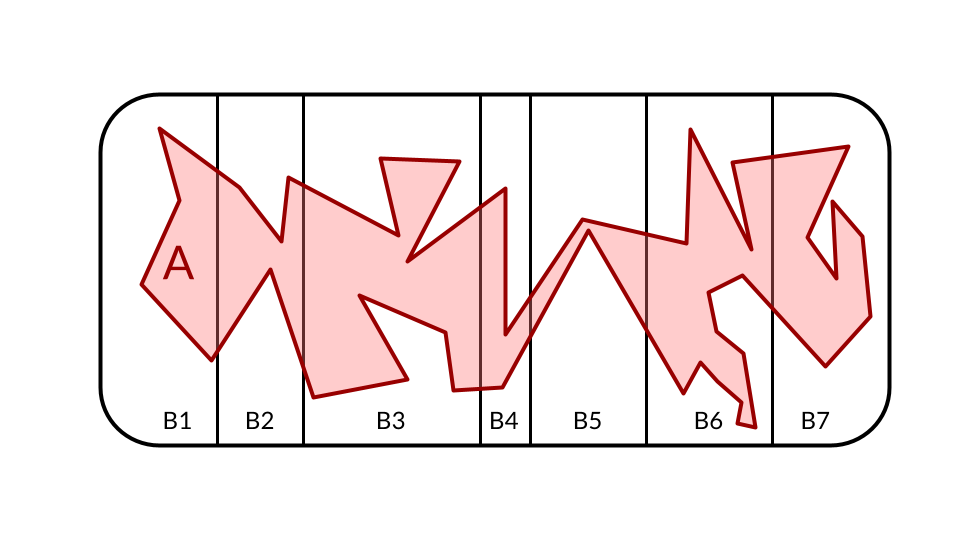
\includegraphics{graphics/ch4-basic-partition.png}

}

\end{figure}%

\begin{tcolorbox}[enhanced jigsaw, rightrule=.15mm, leftrule=.75mm, opacitybacktitle=0.6, title={The Law of Total Probability}, colframe=quarto-callout-tip-color-frame, opacityback=0, coltitle=black, breakable, toptitle=1mm, colbacktitle=quarto-callout-tip-color!10!white, bottomtitle=1mm, titlerule=0mm, arc=.35mm, colback=white, toprule=.15mm, left=2mm, bottomrule=.15mm]

Given a partition, \(B_1, B_2, \dots\), and an event \(A\), the law of
total probability states that
\[P(A) = \sum_i P(A, B_i) = \sum_i P(A|B_i)P(B_i).\]

\end{tcolorbox}

Intuitively, since the whole sample space is divided into the different
\(B_i\)s, this rule breaks down the calculation of \(A\) happening into
manageable chunks. Each term in the summation is ``the probability that
\(A\) happens, given \(B_i\) happening'' weighted by how likely it is
that \(B_i\) happens. Then by summing over all possible \(B_i\), we know
that we must be capturing all possible ways that \(A\) can occur since
all parts of the sample space are contained in exactly one of the sets
of our partition. The law of total probability is an indispensible tool
for computing probabilities in practice.

\begin{example}[Sadie's Possibly Late
Package]\protect\hypertarget{exm-lotp-example}{}\label{exm-lotp-example}

Sadie has still not received the package that Charles had ordered. While
it is not late yet, Charles decides to figure out the probability that
the package will end up being late. Recall that company \(A\) is late
\(75\%\) of the time while company \(B\) is late \(15\%\) of the time,
and the store that Charles ordered from sends out \(10\%\) of packages
with company \(A\), and the rest with company \(B\), which is more
likely.

What is the probability that the package is late?

\begin{tcolorbox}[enhanced jigsaw, colback=white, breakable, rightrule=.15mm, leftrule=.75mm, toprule=.15mm, left=2mm, arc=.35mm, opacityback=0, bottomrule=.15mm]

\vspace{-3mm}\textbf{Solution}\vspace{3mm}

Note that \(A, B\) forms a partition of the sample space as every
package is either sent with \(A\) or with \(B\), and no package can be
sent with both. Further, if \(L\) represents the event that the package
is late, then we know that \(P(L|A) = 0.75\) and \(P(L|B) = 0.15\).
Since \(P(A) = 0.1\) and \(P(B) = 0.9\), an application of the law of
total probability gives
\[P(L) = P(L|A)P(A) + P(L|B)P(B) = (0.75)(0.1) + (0.15)(0.9) = 0.21.\]
As a result, knowing nothing else, the package has a probability of
\(0.21\) of being late.

\end{tcolorbox}

\end{example}

\begin{example}[Charles' Many
Urns]\protect\hypertarget{exm-lotp-example-two}{}\label{exm-lotp-example-two}

While shopping at some garage sales one Sunday morning, Charles and
Sadie stumble across a wonderful find! They see three urns which are
\textbf{exactly} identical to the one that Charles had already purchased
to store the different balls which turned out to not be balls at all.
Realizing the opportunity they splurge and purchase them all, and then
divide the various objects between the four urns, placing all the
spheres in one container, all the cubes in another, all the pyramids in
a third, and all the cones in a fourth.

Once done, they use a different selection mechanism. First, they pick an
urn at random. Next, they random grab one of the items from within it.
The distribution of colours and shapes is included in the following
table.

\begin{longtable}[]{@{}
  >{\raggedright\arraybackslash}p{(\columnwidth - 8\tabcolsep) * \real{0.0588}}
  >{\centering\arraybackslash}p{(\columnwidth - 8\tabcolsep) * \real{0.2353}}
  >{\centering\arraybackslash}p{(\columnwidth - 8\tabcolsep) * \real{0.2353}}
  >{\centering\arraybackslash}p{(\columnwidth - 8\tabcolsep) * \real{0.2353}}
  >{\centering\arraybackslash}p{(\columnwidth - 8\tabcolsep) * \real{0.2353}}@{}}
\toprule\noalign{}
\begin{minipage}[b]{\linewidth}\raggedright
\textbf{Colour}
\end{minipage} & \begin{minipage}[b]{\linewidth}\centering
\textbf{Sphere (Urn 1)}
\end{minipage} & \begin{minipage}[b]{\linewidth}\centering
\textbf{Cube (Urn 2)}
\end{minipage} & \begin{minipage}[b]{\linewidth}\centering
\textbf{Pyramid (Urn 3)}
\end{minipage} & \begin{minipage}[b]{\linewidth}\centering
\textbf{Cone (Urn 4)}
\end{minipage} \\
\midrule\noalign{}
\endhead
\bottomrule\noalign{}
\endlastfoot
\textbf{Red} & 2 & 3 & 2 & 0 \\
\textbf{Blue} & 1 & 0 & 0 & 6 \\
\textbf{Green} & 2 & 2 & 1 & 2 \\
\textbf{Yellow} & 0 & 4 & 2 & 1 \\
\textbf{Black} & 3 & 1 & 1 & 2 \\
\end{longtable}

\begin{enumerate}
\def\labelenumi{\alph{enumi}.}
\tightlist
\item
  What is the probability that they select any of the five colours under
  this sampling scheme?
\item
  How does this change if the probability that each urn is selected is
  proportional to the number of items in it? (Thus, urn 1 is selected
  with probability \(8/35\), and so forth).
\end{enumerate}

\begin{tcolorbox}[enhanced jigsaw, colback=white, breakable, rightrule=.15mm, leftrule=.75mm, toprule=.15mm, left=2mm, arc=.35mm, opacityback=0, bottomrule=.15mm]

\vspace{-3mm}\textbf{Solution}\vspace{3mm}

\begin{enumerate}
\def\labelenumi{\alph{enumi}.}
\item
  Let \(R\), \(B\), \(G\), \(Y\), and \(Bk\) be the events that a red,
  blue, green, yellow, or black ball are selected. Further, let \(U_1\),
  \(U_2\), \(U_3\), and \(U_4\) be the events that the first, second,
  third, or fourth urn are selected. Then note that, according to the
  law of total probability,
  \[P(R) = P(R, U_1) + P(R, U_2) + P(R, U_3) + P(R, U_4) = \sum_{j=1}^4 P(R|U_j)P(U_j).\]
  An equivalent argument holds for each of the other colours. Now,
  \[P(R|U_j) = \frac{N_{R\cap U_j}}{N_{U_j}},\] where \(N_{R\cap U_j}\)
  is the number of red objects in urn \(j\) and \(N_{U_j}\) is the total
  number in urn \(j\). Plugging this in and simplifying we get
  \[P(R) = \sum_{j=1}^4P(R|U_j)\left(\frac{1}{4}\right) = \frac{1}{4}\left\{\frac{2}{8} + \frac{3}{10} + \frac{2}{6}\right\} = \frac{53}{240}.\]

  We can apply analogous arguments to the other colours giving
  \begin{align*}
  P(B) &= \frac{1}{4}\left\{\frac{1}{8} + \frac{6}{11}\right\} = \frac{59}{352} \\
  P(G) &= \frac{1}{4}\left\{\frac{2}{8} + \frac{2}{10} + \frac{1}{6} + \frac{2}{11}\right\} = \frac{527}{2640}\\
  P(Y) &= \frac{1}{4}\left\{\frac{4}{10} + \frac{2}{6} + \frac{1}{11}\right\} = \frac{34}{165}\\
  P(Bk) &= \frac{1}{4}\left\{\frac{3}{8} + \frac{1}{10} + \frac{1}{6} + \frac{2}{11}\right\} = \frac{1087}{5280}.
  \end{align*}

  Note that these probabilities sum to \(1\). In decimal these simplify
  to approximately 0.221, 0.168, 0.2, 0.206, 0.206.
\item
  Using the same setup as before, we have
  \[P(R) = P(R, U_1) + P(R, U_2) + P(R, U_3) + P(R, U_4) = \sum_{j=1}^4 P(R|U_j)P(U_j).\]
  Now \(P(U_1) = 8/35\), \(P(U_2) = 10/35\), \(P(U_3) = 6/35\), and
  \(P(U_4) = 11/35\). Moreover, the conditional probabilities themselves
  do not change, and so instead we have
  \[P(R) = \left\{\frac{2}{8}\cdot\frac{8}{35} + \frac{3}{10}\cdot\frac{10}{35} + \frac{2}{6}\frac{6}{35} + \frac{0}{11}\cdot\frac{11}{35}\right\} = \frac{N_R}{35}.\]
  Note that when multiplying by the marginal probability of the urn, the
  denominator will always cancel. As a result, we end up with the total
  number of reds over \(35\), which leads to \(P(R) = \frac{1}{5}\). The
  same will be true for the other colours, and as a result, if we choose
  the urn based on a weighted selection, this will result in equal
  probability once more.
\end{enumerate}

\end{tcolorbox}

\end{example}

\subsection{Bayes' Theorem}\label{bayes-theorem}

We have seen the direct computation of marginal probabilities (while
using an equally likely outcome model), the computation of conditional
probabilities, the use of the multiplication rule for joint
probabilities, and the use of the law of total probability to indirectly
calculate marginal probabilities through conditioning arguments.
Throughout these discussions we have been primarily concerned with
keeping events \(A\) and \(B\) arbitrary. Everything that we have
indicated for \(P(A)\) holds for \(P(B)\), as does \(P(A|B)\) and
\(P(B|A)\). In reality, it will often be the case that conditioning on
one of the events will be natural, while conditioning on the other will
be more tricky. In these events, it can be useful to be able to
transform statements regarding \(P(A|B)\) into statements regarding
\(P(B|A)\), and vice versa.

Note that because the definitions are symmetric,
\[P(A|B)P(B) = P(A,B) = P(B|A)P(A).\] This is an application of the
multiplication rule in two different orientations. If we divide both
sides of the equality by \(P(B)\), assuming that it is not \(0\), then
we get \[P(A|B) = \frac{P(B|A)P(A)}{P(B)}.\] Now, if we form a
partition, say \(A,A_2,A_3,\dots\), then we can rewrite \(P(B)\) using
the law of total probability as
\[P(B) = P(B|A)P(A) + P(B|A_2)P(A_2) + \cdots = P(B|A)P(A) + \sum_{i=2}P(B|A_i)P(A_i),\]
which can replace \(P(B)\). Taken together this gives a result known as
Bayes' Theorem.\footnote{Bayes' Theorem is named in the same way that
  the Bayesian interpretation of probability is, and that Bayesian
  statistics is more broadly. The connections are more than merely
  surface: Bayes' Theorem can be viewed as the primary technique with
  which we can update subjective beliefs about the world. Importantly,
  however, even those who use a Frequentist view of statistics accept
  the math of Bayes' Theorem, and use it frequently.}

\begin{tcolorbox}[enhanced jigsaw, rightrule=.15mm, leftrule=.75mm, opacitybacktitle=0.6, title={Bayes' Theorem}, colframe=quarto-callout-tip-color-frame, opacityback=0, coltitle=black, breakable, toptitle=1mm, colbacktitle=quarto-callout-tip-color!10!white, bottomtitle=1mm, titlerule=0mm, arc=.35mm, colback=white, toprule=.15mm, left=2mm, bottomrule=.15mm]

Suppose that there are two events, \(A\) and \(B\), with \(P(B) > 0\).
Moreover, suppose that \(A\) taken with \(A_2, A_3, \dots\) forms a
partition. Then Bayes' Theorem states that
\[P(A|B) = \frac{P(B|A)P(A)}{P(B)} = \frac{P(B|A)P(A)}{P(B|A)P(A) + \sum_{i=2} P(B|A_i)P(A_i)}.\]

\end{tcolorbox}

Bayes' Theorem allows us to convert statements regarding \(P(B|A)\) into
statements regarding \(P(A|B)\). Note that, as we derived above, Bayes'
Theorem is an application of the multiplication rule and an application
of the law of total probability.\footnote{In fact, I would go as far as
  to suggest that learning Bayes' Theorem by itself is less important
  than fully grasping the definition of conditional probability
  alongside the multiplication rule and the law of total probability. I
  myself do not remember Bayes' Theorem directly, but can write it down
  directly from these definitions without any thought.} Sometimes we may
have \(P(B)\) directly, rendering the law of total probability in the
denominator unnecessary.

Often, the natural partition to select when we do need the law of total
probability is to take \(A\) and \(A^C\). Note that any set with its
complement forms a partition, since by definition they occupy the entire
space and are non-overlapping. When this is done we get the slightly
more compact relationship of
\[P(A|B) = \frac{P(B|A)P(A)}{P(B|A)P(A) + P(B|A^C)P(A^C)}.\]

Bayes' Theorem differs from our previous relationships as it allows us
to translate one set of conditional probabilities into another. Every
other relationship we have looked at has moved between types of
probabilities, whereas Bayes' Theorem deals directly with conditional
relationships.

The most commonly cited example application is in medical testing.
Suppose that we know the performance characteristics of a particular
medical test: it is \(99\%\) accurate for positive cases, and \(95\%\)
accurate for negative cases. That is, with probability \(0.99\) it
correctly returns positive when an individual is infected, and with
probability \(0.95\) it returns negative when an individual is not
infected.These are both statements of conditional probability. If we
take \(A\) to be the event that the test returns positive, and \(B\) to
be the event that the patient is infected,\footnote{It is worth drawing
  attention to the language that we have started to use at this point in
  the notes regarding ``events''. In this case our sample space would
  actually be formed using pairs of information. In particular, we might
  have
  \[\mathcal{S} = \{(\text{Pos. Test}, \text{Illness}), (\text{Neg. Test}, \text{Illness}),(\text{Pos. Test}, \text{No Illness}),(\text{Neg. Test}, \text{No Illness})\}.\]
  Then the event \(A\) here is actually
  \(A = \{(\text{Pos. Test}, \text{Illness}),(\text{Pos. Test}, \text{No Illness})\}\)
  and \(B\) is
  \(\{(\text{Pos. Test}, \text{Illness}),(\text{Neg. Test}, \text{Illness})\}\).
  It is far more clunky to make explicit these events, and so we move
  towards using more natural language. Until you feel confident that you
  can identify the specific outcomes associated with the events of
  interest, it is worth writing these out in full.} then we are saying
that \(P(A|B) = 0.99\) and \(P(A^C|B^C) = 0.95\) which means that
\(P(A|B^C) = 0.05\). Suppose that we know that, across the entire
population, one in a thousand individuals is likely to be infected. This
means that \(P(B) = 0.001\).

Now if a random individual goes into a doctor's office and tests
positive for the disease, how likely are they to actually be infected?
In this case we want to know the probability of them being infected
given that they have tested positive. In notation, this is \(P(B|A)\).
We do not know this quantity directly, but given an application of
Bayes' Theorem, we can find it. Using the natural partition of \(B\) and
\(B^C\), we get
\[P(B|A) = \frac{P(A|B)P(A)}{P(A|B)P(B)+P(A|B^C)P(B^C)} = \frac{(0.99)(0.001)}{(0.99)(0.001)+(0.05)(0.999)} \approx 0.019.\]
That is, despite the fact that this test is exceptionally effective at
detecting this disease, a positive test still means that an individual
has a probability of only \(0.019\) of actually having the
illness.\footnote{This counter intuitive fact was an intensely
  frustrating reality for statisticians everywhere during the height of
  the COVID-19 pandemic, when politicians and the population at large
  turned away from testing owing to its perceived ``ineffectiveness''.
  The quantity of interest for knowing how good a test is is \(P(A|B)\)
  and \(P(A^C|B^C)\). However, if a disease is sufficiently rare, with
  \(P(B)\) sufficiently small, then no matter how effective the tests
  are you will likely have \(P(B|A)\) to be low. Note that
  \(P(B|A) >> P(B)\) in the example, and this will also be true in
  general. A single test cannot say with certainty, however, they are an
  incredibly effective tool at reducing our uncertainty.}

\begin{example}[Sadie's Late
Package]\protect\hypertarget{exm-bayes-theorem}{}\label{exm-bayes-theorem}

Sadie eventually received the package that Charles had sent, but it
arrived very late. Sadie was not home when the package was delivered and
there no obvious markings on the box to indicate which of the two
delivery companies had sent it.

Given this information, and knowing that company \(A\) is late \(75\%\)
of the time while company \(B\) is late \(15\%\) of the time, and the
store that Charles ordered from sends out \(10\%\) of packages with
company \(A\), and the rest with company \(B\), what is the probability
that the package was delivered by each of the two companies?

\begin{tcolorbox}[enhanced jigsaw, colback=white, breakable, rightrule=.15mm, leftrule=.75mm, toprule=.15mm, left=2mm, arc=.35mm, opacityback=0, bottomrule=.15mm]

\vspace{-3mm}\textbf{Solution}\vspace{3mm}

We want to determine \(P(A|L)\) and \(P(B|L)\). We know that
\(P(L|A) = 0.75\) and \(P(L|B) = 0.15\). Moreover, we know that
\(P(A) = 0.1\) and \(P(B) = 0.9\). Applying Bayes' Theorem directly we
get
\[P(A|L) = \frac{P(L|A)P(A)}{P(L|A)P(A) + P(L|B)P(B)} = \frac{(0.75)(0.10)}{(0.75)(0.10) + (.10)(0.90)} = \frac{5}{11}.\]
Similarly, we get
\[P(B|L) = \frac{P(B|A)P(B)}{P(L|A)P(A) + P(L|B)P(B)} = \frac{(0.15)(0.90)}{(0.75)(0.10) + (.10)(0.90)} = \frac{6}{11}.\]
Note, we could have also used the fact that \(P(A|L) + P(B|L) = 1\) to
determine this. As a result, it is more likely that \(B\) delivered the
package than \(A\).\footnotemark{}

\end{tcolorbox}

\footnotetext{Note that this is another example of a counterintuitive
result. Here, \(A\) is far more likely to be late, but it is more likely
that \(B\) delivered a late package to us than \(A\) because of the
\textbf{base rates}. That is, \(P(B)\) is much higher to begin than
\(P(A)\), and so that is hard to overcome. It is worth noting, however,
that originally \(P(B)\) is \(9\) times more likely than \(P(A)\), and
after knowing that package is late it is \(\frac{6}{5} = 1.2\) times
more likely. This major reduction in the relative likelihood is owed to
how much more likely \(A\) is to deliver late packages than \(B\).}

\end{example}

Bayes' Theorem highlights a key lesson when considering conditional
probabilities, and it's a common mistake to make which should be avoided
at all costs. Namely, we cannot interchange \(P(A|B)\) with \(P(B|A)\).
These probabilities are not necessarily highly correlated with one
another, and it is important to distinguish clearly which is the
probability of interest.\footnote{Mixing up \(P(B|A)\) and \(P(A|B)\) is
  often called \emph{confusion of the inverse}, and it can lead to very
  faulty conclusions when ignored. In the medical testing example above,
  it is important to not confuse ``the probability that the test returns
  positive, assuming you have the illness'' with ``the probability that
  you have the illness, given that the test returns positive.'' This
  type of faulty logic has long been used to justify discriminatory
  behaviour in medicine, the law, and so on. A thorough understanding of
  statistics and probability helps to ensure that these types of errors
  are not made, and gives you the tools to push-back on the spots where
  people are making these arguments incorrectly, particularly when the
  stakes are high or harm is being done.} The stakes of these types of
confusion can be quite high, and it is tremendously important to ensure
that you are conditioning on the correct events. Fortunately, Bayes'
Theorem allows us to translate between events for conditioning, giving a
mechanism from translating between the two.\footnote{When discussing
  Bayes' Theorem we introduced two frequently occurring sources of error
  when reasoning about probabilities, and showed how to remedy them.
  \emph{Confusion of the inverse} occurs when you mix up \(P(A|B)\) with
  \(P(B|A)\), and can lead to disastrous consequences. The \emph{base
  rate fallacy} occurs when you fail to take into account the rareness
  of the marginal events and instead only consider the conditionals
  (such as seeing that delivery company \(A\) was more likely to be late
  than \(B\), without considering that \(B\) was more likely to be used
  than \(A\)). These are both examples of the challenges at the heart of
  probability and statistics: namely, the subjects are fairly
  unintuitive once moving beyond the basics. As a result, we need to
  rely on building up our intuitions over time by making use of the
  formal rules that we are able to derive.}

\section{Independence}\label{independence}

We have seen that, in most cases, conditioning on an event changes the
probability of that event. For instance, if we want to know the
probability it is raining, if we condition on knowing that it is a day
full of gray skies, the conditional probability is likely higher than
the marginal probability. By considering how the marginal and
conditional probabilities differ, we are in effect indicating a
dependence of the events on one another. In terms of probability, this
dependence is captured by an influence on the degree of uncertainty
present depending on what we know.

It is totally possible that two events do not influence one another at
all. The weather outside today is likely not influenced by your
favourite sports team's performance last night.\footnote{Though, perhaps
  the world will freeze over if
  \emph{(insert-your-least-favourite-team-here)} wins the
  \emph{(insert-the-name-of-the-championship-for-the-league-you-care-about-here)}?}
In this case, we would have \(P(A|B) = P(A)\).

We saw an example of this previously when we wanted to know the
probability of a randomly selected card being a heart (\(A\)) given that
it was an ace (\(B\)). We found that this was \(\frac{1}{4}\), exactly
the same as the probability if we did not know that it was an ace. Thus
here we have \(P(A|B)=P(A)\). We could have also said that
\(P(B|A)=P(B)=\frac{1}{13}\). The symmetry of these events makes it
somewhat more convenient to express this relationship differently.

Instead of writing \(P(A|B) = P(A)\) and \(P(B|A) = P(B)\), we can
multiply the first relationship by \(P(B)\) on both sides, or the second
by \(P(A)\) on both sides. The multiplication rule gives
\(P(A|B)P(B) = P(A,B)\), and so the first relationship becomes
\(P(A,B) = P(A)P(B)\). The second follows exactly the same. Any two
events that satisfy this relationship are said to be independent.

\begin{definition}[Independence]\protect\hypertarget{def-independence}{}\label{def-independence}

Any two events, \(A\) and \(B\), which satisfy \(P(A,B) = P(A)P(B)\) are
said to be independent. If \(A\) and \(B\) are independent we write
\(A\perp B\), and read ``\(A\) is independent of \(B\)''. Any events
which are not independent are said to be dependent, and we write
\(A\not\perp B\).

\end{definition}

Note that independence is always a symmetric property: if \(A\) is
independent of \(B\), then \(B\) is independent of \(A\). To check
whether two events are independent, we check whether their joint
probability is equal to the product of their marginal probabilities.

\begin{tcolorbox}[enhanced jigsaw, rightrule=.15mm, leftrule=.75mm, opacitybacktitle=0.6, title={Properties of Independence}, colframe=quarto-callout-warning-color-frame, opacityback=0, coltitle=black, breakable, toptitle=1mm, colbacktitle=quarto-callout-warning-color!10!white, bottomtitle=1mm, titlerule=0mm, arc=.35mm, colback=white, toprule=.15mm, left=2mm, bottomrule=.15mm]

Note that if \(A\perp B\), then \(A^C\perp B\), \(A^C\perp B^C\), and
vice versa. To see this note \[P(A^C, B) + P(A, B) = P(B),\] by the Law
of Total Probability. Then, by independence of \(A\) and \(B\) this
gives \begin{align*}
P(A^C, B) + P(A)P(B) &= P(B) \\
\implies P(A^C, B) &= P(B) - P(A)P(B) \\
&= P(B)(1 - P(A)) \\
&= P(B)P(A^C),\end{align*} as is required. The other combinations follow
in the same manner.

\end{tcolorbox}

If \(P(A)\neq 0\), then we can divide both sides by \(P(A)\) to gives
\(P(B|A) = P(B)\). Similarly, if \(P(B)\neq 0\), then we can divide both
sides by \(P(B)\) to give \(P(A|B)=P(A)\). This expression in terms of
conditional probabilities is the more intuitive expression of
independence. It directly captures the idea that ``knowing \(B\) does
not change our belief about \(A\)''. However, we must be careful. This
conditional argument is only valid when the event that is being
conditioned on is not probability \(0\), where the defining
relationship, \(P(A,B) = P(A)P(B)\), will hold for all events. Recall
that, in general, \(P(A\cap B) = P(A)+P(B)-P(A\cup B)\). It is only when
assuming independence that this simplifies further.

\begin{example}[Independence and Board
Games]\protect\hypertarget{exm-assessing-independence}{}\label{exm-assessing-independence}

Charles and Sadie are invited over to a friends house, Garth, to play
some board games. Both of them are quite excited by this prospect as
board games feel like the next logical step for the two of them, being
as into probability and games as they are! Garth has a large board game
collection, and begins to explain the games to Charles and Sadie across
a variety of axes:

\begin{itemize}
\tightlist
\item
  Whether the games are competitive or cooperative.
\item
  How many players the games play best at (\(\{1, 2, 3, 4+\}\)).
\item
  How ``heavy'' the games tend to be (friendly for everyone, moderately
  involved, or very heavy).
\end{itemize}

While Garth continues on about several other topics including the
themes, the mechanics, or the rating on BoardGameGeek, Charles drifts
off wondering whether the traits listed are independent in Garth's
collection. Suppose that Garth has \(100\) games, of which:

\begin{itemize}
\tightlist
\item
  \(25\) are cooperative.
\item
  \(5\) are best played at one player, \(20\) at two, and \(55\) at
  three.
\item
  \(10\) are friendly for everyone and \(45\) are moderately involved.
\end{itemize}

\begin{enumerate}
\def\labelenumi{\alph{enumi}.}
\tightlist
\item
  If \(5\) games are best played at two players and are cooperative, are
  these events independent?
\item
  If \(20\) games are heavy and best played with \(4+\) players, are
  these events independent?
\item
  If \(0\) games are both moderately involved and cooperative, are these
  events independent?
\item
  Charles figures that competitive games and two player games are
  independent. How many competitive two player games are there?
\item
  Is it possible that competitive games are independent of heavy games?
\end{enumerate}

\begin{tcolorbox}[enhanced jigsaw, colback=white, breakable, rightrule=.15mm, leftrule=.75mm, toprule=.15mm, left=2mm, arc=.35mm, opacityback=0, bottomrule=.15mm]

\vspace{-3mm}\textbf{Solution}\vspace{3mm}

\begin{enumerate}
\def\labelenumi{\alph{enumi}.}
\item
  We are suggesting that \(P(A,B) = 0.05\), where \(A\) is ``two
  player'' and \(B\) is ``cooperative''. We know that \(P(B) = 0.25\)
  and \(P(A) = 0.20\). Calculating
  \(P(A)P(B) = (0.20)(0.25) = 0.05 = P(A,B)\), and so these traits
  \textbf{are} independent.
\item
  We have \(P(A,B) = 0.2\) where \(A\) is ``heavy'' and \(B\) is
  ``\(4+\) players. We know that \(P(A) = 0.45\) and \(P(B) = 0.20\),
  and so \(P(A)P(B) = (0.45)(0.20) = 0.09 \neq P(A,B)\). As a result,
  these traits are \textbf{not} independent.
\item
  We know that \(P(A) > 0\) and \(P(B) > 0\) for \(A\) being moderately
  involved and \(B\) being cooperative. As a result, \(P(A)P(B) > 0\),
  and so if \(P(A,B) = 0\), they must \textbf{not} be independent.
\item
  Taking \(A\) to be ``competitive'' we have \(P(A) = 0.75\). Taking
  \(B\) to be ``two player'' we have \(P(B) = 0.20\). As a result, if
  \(A\perp B\) then \(P(A,B) = P(A)P(B) = (0.75)(0.20) = 0.15\). Thus,
  there must be \(15\) competitive, two player games.
\item
  Taking \(A\) to be ``competitive'' we have \(P(A) = 0.75\). Taking
  \(B\) to be ``heavy'' weh ave \(P(B) = 0.45\). Thus, if they were
  independent, we would have
  \(P(A,B) = P(A)P(B) = (0.75)(0.45) = 0.3375\). This would require
  \(33.75\) games to be heavy, competitive games and so we must conclude
  that they are \textbf{not} independent.
\end{enumerate}

\end{tcolorbox}

\end{example}

\subsubsection{Mutually Exclusive
Events}\label{mutually-exclusive-events}

Importantly, if \(A\perp B\), then \(A\cap B\neq \emptyset\) unless
either \(A=\emptyset\), \(B=\emptyset\), or both. To see this recall
that \(P(\emptyset) = 0\), and so if \(A\cap B = \emptyset\) then
\(P(A\cap B) = P(A)P(B) = P(\emptyset) = 0\). This only holds if either
\(P(A) = 0\) or \(P(B) = 0\). This may seem to be a rather technical
point, however, it is the source of much confusion regarding
independence. In particular, it is common to mistake independent events
for mutually exclusive events.

\begin{definition}[Mutually Exclusive
Events]\protect\hypertarget{def-mutually-exclusive-events}{}\label{def-mutually-exclusive-events}

Two events, \(A\) and \(B\) are said to be mutually exclusive if they
are disjoint. In particular, if \(P(A,B) = 0\) then \(A\) and \(B\) are
mutually exclusive. If \(A\) and \(B\) are mutually exclusive events,
with \(P(A) > 0\) and \(P(B) > 0\), then \(A\not\perp B\).

\end{definition}

Whenever only one event from a set of events can happen, we refer to the
events as being mutually exclusive. If one happens, we know that the
others did not. Mutually exclusive events are always dependent since
knowing that \(A\) occurs dramatically shifts our belief about
\(B\),\(C\), and \(D\).\footnote{Namely, we know that all of the others
  are then impossible.}

The primary concern with mutually exclusive and independent events is a
linguistic one. We often use words like independent to mean unrelated,
and in a sense, mutually exclusive events are unrelated in that one has
nothing to do with another. However, in statistics and probability, when
we discuss independence, it is not an independence of the events
themselves but rather an independence relating to our beliefs regarding
the uncertainty associated with the events. In this sense, mutually
exclusive events are very informative regarding the uncertainty
associated with them.

\begin{example}[Charles and Sadie Cooking
Dinner]\protect\hypertarget{exm-independence-two}{}\label{exm-independence-two}

Suppose that Charles and Sadie always eat dinner together. It will
either be the case that Charles cooks at home, that Sadie cooks at home,
that the two of them order in, or that they go out to eat. If we take
these to be four events, \(A\), \(B\), \(C\), and \(D\), then are any of
these events independent? Mutually exclusive? Explain.

\begin{tcolorbox}[enhanced jigsaw, colback=white, breakable, rightrule=.15mm, leftrule=.75mm, toprule=.15mm, left=2mm, arc=.35mm, opacityback=0, bottomrule=.15mm]

\vspace{-3mm}\textbf{Solution}\vspace{3mm}

Assuming, as it seems reasonable given the information in the question,
that only one of the possible tasks occurs for dinner in a night, then
we \emph{know} that
\[P(A,B) = P(A,C) = P(A,D) = P(B,C) = P(B,D) = P(C,D) = 0.\] As a
result, all of the events described are mutually exclusive, and
correspondingly, are \emph{not} independent.

\end{tcolorbox}

\end{example}

\section{Contingency Tables}\label{contingency-tables}

Through to this point we have discussed probabilities in the abstract,
either through an enumeration of equally likely outcomes, or else by
directly specifying the likelihood of various events. While these are
useful in many regards, we are often looking for more concise manners of
summarizing information of interest. One tool for accomplishing this is
a contingency table.

\begin{definition}[Contingency
Table]\protect\hypertarget{def-contingency-table}{}\label{def-contingency-table}

A contingency table is a tabular summary of information which summarizes
the joint probabilities of two or more variables. Typically a
contingency table will take one factor for the columns and a secondary
factor for the rows, where each cell then represents the frequency with
which observations occur in the two corresponding categories
simultaneously.

\end{definition}

To begin, you could imagine constructing a frequency table relaying the
frequency with which undergraduate students are enrolled in various
faculties at a particular university. This tells you, of the whole
population of students at the university, what is the faculty breakdown.
By dividing the number in each faculty by the total number of students,
you convert the frequencies to proportions, and these proportions can be
viewed as probabilities. (See Table~\ref{tbl-uni-frequency}.\footnote{Note,
  the values in this table are \emph{roughly} inspired by a subset of
  the
  \href{https://web.archive.org/web/20240103124753/https://www.unb.ca/finance/_assets/documents/rpb/factbooktables/2022enrollment/20221215-tablee3-enrolment-ftehc-fac-acad-lvl-2022fa-final.pdf}{Fall
  2022 University of New Brunswick Enrolment Numbers}.}) The
interpretation of proportions as probabilities implies a very specific
statistical experiment. In particular, the proportion represents the
probability that an individual selected at random from the entire
population has the given trait. This is frequently a probability of
interest, which makes these summary tables a useful tool.\footnote{This
  provides further emphasis for the utility of urn models. If you
  imagine an urn that has balls with two or more traits (say like those
  in Example~\ref{exm-conditional-probability-urn}), then randomly
  selecting a single ball from this population has an analogous
  probability distribution.}

\begin{table}

\caption{\label{tbl-uni-frequency}Frequency and corresponding
proportions of enrolment by faculty in a university.}

\centering{

\begin{tabular}{>{}l|r|r}
\hline
Faculty & Enrolment & Proportion\\
\hline
\textbf{Arts} & 1266 & 0.2182382\\
\hline
\textbf{Computer Science} & 749 & 0.1291157\\
\hline
\textbf{Education} & 786 & 0.1354939\\
\hline
\textbf{Engineering} & 1315 & 0.2266851\\
\hline
\textbf{Law} & 266 & 0.0458542\\
\hline
\textbf{Nursing} & 543 & 0.0936046\\
\hline
\textbf{Science} & 876 & 0.1510084\\
\hline
\hline
\textbf{\textbf{Total}} & \textbf{5801} & \textbf{1.0000000}\\
\hline
\end{tabular}

}

\end{table}%

When a single trait is displayed we refer to these tabular summaries as
frequency tables or frequency distributions. A contingency table instead
plots two or more traits on the same table, with each cell representing
the frequency of both traits occurring simultaneously in the population.
Extending the university example, we may further include the student's
current year of study to see the breakdown of both faculty and year of
study, in one table.

\begin{table}

\caption{\label{tbl-uni-contingency}Frequency of enrolment by faculty
and year of study in a university.}

\centering{

\begin{tabular}{>{}l|c|c|c|c|c|>{}c}
\hline
  & Year 1 & Year 2 & Year 3 & Year 4 & Year 5+ & \\
\hline
\textbf{Arts} & 222 & 276 & 273 & 225 & 270 & \textbf{1266}\\
\hline
\textbf{Comp. Sci.} & 164 & 87 & 164 & 90 & 244 & \textbf{749}\\
\hline
\textbf{Education} & 100 & 136 & 184 & 128 & 238 & \textbf{786}\\
\hline
\textbf{Engineering} & 189 & 290 & 354 & 298 & 184 & \textbf{1315}\\
\hline
\textbf{Law} & 54 & 50 & 58 & 37 & 67 & \textbf{266}\\
\hline
\textbf{Nursing} & 55 & 90 & 154 & 112 & 132 & \textbf{543}\\
\hline
\textbf{Science} & 242 & 114 & 206 & 183 & 131 & \textbf{876}\\
\hline
\hline
\textbf{\textbf{}} & \textbf{1026} & \textbf{1043} & \textbf{1393} & \textbf{1073} & \textbf{1266} & \textbf{\textbf{5801}}\\
\hline
\end{tabular}

}

\end{table}%

By including two (or more) factors in the table we are able to capture
not only the marginal probabilities for the population, but also the
joint probabilities for the population, and in turn, the conditional
probabilities for the population. Being able to concisely summarize all
of these concepts regarding traits in a population of interest renders
contingency tables immensely useful in the study of uncertainty broadly.

Consider the two-way contingency table, Table~\ref{tbl-uni-contingency}.
Each cell consists of frequency with which a combination of the two
traits occurs in the population.\footnote{That is, the number of
  students who are enrolled in that faculty, in that year of study.} If
we take events corresponding to each of the levels of the two variables
of interest, then these central cells represent the frequency of joint
events. That is, each interior cell gives the total number of
observations with a set level for variable one\footnote{Faculty.} AND a
set level for variable two\footnote{Year of study.}. For instance, there
are 50 individuals who are in Law and studying in Year 2.

Each row is then summed, with the total number following into the
corresponding row recorded in the right hand margin. each column is
summed, with the total number corresponding to the given column recorded
in the bottom margin. For instance there are a total of 786 students in
Education and a total of 1393 in Year 3. Then the margin totals are
summed and the total is recorded in the lower right margin space (in
this case, 5801). Whether the rows or columns are summed, they should
sum to the same total, which is the total of the population under
consideration. This is the same as simply adding all of the observed
interior frequencies. To turn a frequency into a probability, you need
only divide the correct frequency by the correct total.

\begin{table}

\caption{\label{tbl-uni-prop}Proportions of enrolment by faculty and
year of study in a university.}

\centering{

\begin{tabular}{>{}l|c|c|c|c|c|>{}c}
\hline
  & Year 1 & Year 2 & Year 3 & Year 4 & Year 5+ & \\
\hline
\textbf{Arts} & 0.0382693 & 0.0475780 & 0.0470609 & 0.0387864 & 0.0465437 & \textbf{0.2182382}\\
\hline
\textbf{Comp. Sci.} & 0.0282710 & 0.0149974 & 0.0282710 & 0.0155146 & 0.0420617 & \textbf{0.1291157}\\
\hline
\textbf{Education} & 0.0172384 & 0.0234442 & 0.0317187 & 0.0220652 & 0.0410274 & \textbf{0.1354939}\\
\hline
\textbf{Engineering} & 0.0325806 & 0.0499914 & 0.0610240 & 0.0513705 & 0.0317187 & \textbf{0.2266851}\\
\hline
\textbf{Law} & 0.0093087 & 0.0086192 & 0.0099983 & 0.0063782 & 0.0115497 & \textbf{0.0458542}\\
\hline
\textbf{Nursing} & 0.0094811 & 0.0155146 & 0.0265471 & 0.0193070 & 0.0227547 & \textbf{0.0936046}\\
\hline
\textbf{Science} & 0.0417169 & 0.0196518 & 0.0355111 & 0.0315463 & 0.0225823 & \textbf{0.1510084}\\
\hline
\hline
\textbf{\textbf{}} & \textbf{0.1768661} & \textbf{0.1797966} & \textbf{0.2401310} & \textbf{0.1849681} & \textbf{0.2182382} & \textbf{\textbf{1.0000000}}\\
\hline
\end{tabular}

}

\end{table}%

For the standard joint probabilities, you take the interior cell count
and divide by the population total. Here we are saying that some fixed
number, \(m\), of the \(N\) total individuals have both traits under
consideration. For instance, the joint probability that a student is in
Law and studying in Year 2 is 0.0086192.\footnote{It is worth
  reemphasizing what this probability actually means. If we were to
  randomly sample, with equal probability, individuals from this
  population then the probability that an individual selected has both
  the faculty and year specified is given by the joint probability. That
  is to say, if we did this over and over and over again (with
  replacement) in the long-term, these probabilities represent
  proportion of time those combinations would be observed.} If instead
you wish to find a marginal probability, you have to consider the value
in the corresponding margin: this is the total number of individuals
with the given trait, ignoring the level of the other variable. These
marginal values are also divided by the total population size. For
instance, there is a 0.1354939 probability of observing a student in
Education and a probability 0.240131 of observing a student in Year 3.

Outside of joint and marginal probabilities, we can also find
conditional probabilities. To do so, we restrict our focus to either
only one row, or one column. Then, we can take the joint cell and divide
by the value in the margin, which gives the conditional probability of
interest. Note, this works with \emph{either} the contingency table
directly \textbf{or} with the propensity table. The reasoning is that
the propensity table divided by the same totals in the numerator and the
denominator. Suppose we take some cell, \(A\cap B\), which has
\(N_{A, B}\) in the contingency table. Then,
\[P(A\cap B) = \frac{N_{A, B}}{N} \quad\quad\text{and}\quad\quad P(B) = \frac{N_B}{N}.\]
If we consider then forming \(P(A|B)\) we get
\[P(A|B) = \frac{P(A \cap B)}{P(B)} = \frac{N_{A \cap B}/\cancel{N}}{N_B/\cancel{N}} = \frac{N_{A, B}}{N_B}.\]
Thus, given that we know a student is in Education, then the probability
that they are in Year 3 is approximately 0.2341.

Note that these procedures are exactly in line with what we had seen
before. The conditional probability is defined as the joint probability
divided by the marginal probability. The process of computing the
marginal can be seen as an application of the law of total probability.
As a result, contingency tables can be a useful, tangible tool for
investigating the techniques we have been discussing: they are not a
substitute for direct manipulation of the mathematical objects, but they
can present insight into the underlying processes where it may be hard
to derive that insight otherwise.

\begin{tcolorbox}[enhanced jigsaw, rightrule=.15mm, leftrule=.75mm, opacitybacktitle=0.6, title={The Law of Total Probability: Contingency Table's Version}, colframe=quarto-callout-warning-color-frame, opacityback=0, coltitle=black, breakable, toptitle=1mm, colbacktitle=quarto-callout-warning-color!10!white, bottomtitle=1mm, titlerule=0mm, arc=.35mm, colback=white, toprule=.15mm, left=2mm, bottomrule=.15mm]

Recall that the law of total probability states that, if
\(B_1,\dots,B_n\) forms a partition of the sample space, then
\[P(A) = \sum_{i=1}^n P(A|B_i)P(B_i) = \sum_{i=1}^n P(A, B_i)\]. In a
contingency table it is easier to see how either of the two factors at
play (either those in the rows or the columns) forms a partition of the
space. Every observation has to fall in exactly one row and exactly one
column. Thus, if we want to know the marginal frequency of a single
trait (say represented by some row of the table), then one way to find
this total is to sum up every observation in each of the corresponding
columns. This is \emph{precisely} the same process as the law of total
probability. Note that, denoting each column as \(B_i\), and supposing
there are \(k\) total columns, then the total number in a row is taken
to be \[N_A = \sum_{i=1}^k N_{A, B_i},\] simply as the summation of the
corresponding row. By definition, \(P(A) = \frac{N_A}{N}\), and so
dividing both sides by \(N\) gives
\[P(A) = \frac{N_A}{N} = \frac{1}{N}\sum_{i=1}^k N_{A, B_i} = \sum_{i=1}^k \frac{N_{A, B_i}}{N} = \sum_{i=1}^n P(A\cap B_i).\]

\end{tcolorbox}

It is important to note that there is redundant information within a
contingency table. For instance, the margins need not be listed
explicitly, as they can be directly calculated from the interior points.
Same goes for interior points, given the margins of the table (assuming
\emph{some} interior points are also presented). This can be useful for
a compact representation of the information, and manipulating these
tables -- being able to find the required information in many places --
should become familiar to you as you continue to work with them more and
more.

\begin{example}[The Evolving Contents of Charle's
Urns]\protect\hypertarget{exm-charles-contingency-table}{}\label{exm-charles-contingency-table}

After learning of contingency tables, Sadie points out to Charles that
with the whole urn debacle they went through, the two of them actually
ended up using a contingency table to summarize the information. How
neat! In the interim, there has been some development in the contents of
Charles's urns, and armed with the new knowledge of contingency tables,
the following summary is produced.

\begin{tabular}{>{}l|c|c|c|c|>{}c}
\hline
  & Cone & Cube & Pyramid & Sphere & \\
\hline
\textbf{Black} & 2 & A & 1 & 3 & \textbf{10}\\
\hline
\textbf{Blue} & 1 & 2 & 1 & 1 & \textbf{5}\\
\hline
\textbf{Green} & 3 & 3 & B & 5 & \textbf{15}\\
\hline
\textbf{Red} & 2 & C & 3 & 2 & \textbf{D}\\
\hline
\textbf{Yellow} & 5 & 3 & 4 & 1 & \textbf{13}\\
\hline
\textbf{\textbf{}} & \textbf{13} & \textbf{E} & \textbf{13} & \textbf{12} & \textbf{\textbf{50}}\\
\hline
\end{tabular}

Sadly, Charles does not have the best writing and Sadie cannot make out
what values were written in for the cells marked \(A\), \(B\), \(C\),
\(D\), and \(E\).

\begin{enumerate}
\def\labelenumi{\alph{enumi}.}
\tightlist
\item
  What are the values for the missing values?
\item
  What is the probability that a black cube is drawn?
\item
  What is the probability that a red object is drawn?
\item
  What is the probability that a cube is drawn?
\item
  Given that the drawn object was a pyramid, what is the probability
  that it is green?
\item
  Given that the object is green, what is the probability that it is a
  pyramid.
\end{enumerate}

\begin{tcolorbox}[enhanced jigsaw, colback=white, breakable, rightrule=.15mm, leftrule=.75mm, toprule=.15mm, left=2mm, arc=.35mm, opacityback=0, bottomrule=.15mm]

\vspace{-3mm}\textbf{Solution}\vspace{3mm}

\begin{enumerate}
\def\labelenumi{\alph{enumi}.}
\item
  We start by filling in the missing cells, in order.

  \begin{enumerate}
  \def\labelenumii{\roman{enumii}.}
  \item
    For \(A\) we can note that \(2 + A + 1 + 3 = 10\), which gives that
    \(A = 4\). We could have also tried a column sum, however, this
    would involve \(3\) unknowns and so would not have given a numeric
    result.
  \item
    For \(B\) either a row sum or column sum would produce the correct
    answer. We either take \(3 + 3 + B + 5 = 15\) giving \(B = 4\) or
    \(1 + 1 + B + 3 + 4 = 13\) giving \(B=4\).
  \item
    \(C\) is more challenging as we either have that
    \(2 + C + 3 + 2 = D\) or \(4 + 2 + 3 + C + 3 = E\)\footnotemark{} As
    a result, for this technique we will need to find either \(D\) or
    \(E\) first. There is an alternative technique to use, which would
    be to note that we have \emph{all} the internal points specified at
    this point, and we know that these sum to \(50\). As a result, we
    could note that \(C = 50 - 10 - 5 - 15 - 13 - 2 - 3 - 2 = 0\) or
    that \(C =  50 - 13 - 13 - 12 - 4 - 2 - 3 - 3 = 0\).
  \item
    We can find \(D\) either by subtracting from the total,
    \(D = 50 - 10 - 5 - 15 - 13 = 7\), or by adding along the row,
    \(2 + 0 + 3 + 2 = 7\).\footnotemark{} Note that with \(D = 7\), had
    we not found \(C = 0\) above, we could now take
    \(2 + C + 3 + 2 = 7\) and find \(C = 0\).
  \item
    Like \(D\), we have two options for working this out. Either
    \(E = 50 - 13 - 13 - 12 = 12\) or
    \(E = 4 + 2 + 3 + 0 + 3 = 12\).\footnotemark{} Like with \(D\), had
    we solved for \(E\) first, then we could find \(C\) via
    \(4 + 2 + 3 + C + 3 = 12\).
  \end{enumerate}
\item
  Here we want \(P(\text{Black}, \text{Cube})\). This is given by the
  frequency of black cubes divided by \(50\). Thus,
  \[P(\text{Black}, \text{Cube}) = \frac{A}{50} = \frac{4}{50} = 0.08.\]
\item
  Here we want \(P(\text{Red})\). This is given by the marginal
  frequency of red objects divided by \(50\). Thus,
  \[P(\text{Red}) = \frac{D}{50} = \frac{7}{50} = 0.14.\]
\item
  Here we want \(P(\text{Cube})\). This is given by the marginal
  frequency of cubes divided by \(50\). Thus,
  \[P(\text{Cube}) = \frac{E}{50} = \frac{12}{50} = 0.24.\]
\item
  Here we want \(P(\text{Green}|\text{Pyramid})\). This is given by the
  frequency of green pyramids divided by the marginal frequency of
  pyramids. Thus
  \[P(\text{Green}|\text{Pyramid}) = \frac{B}{13} = \frac{4}{13} \approx 0.308.\]
\item
  Here we want \(P(\text{Pyramid}|\text{Green})\). This is given by the
  frequency of green pyramids divided by the marginal frequency of green
  objects.\footnotemark{} Thus
  \[P(\text{Pyramid}|\text{Green}) = \frac{B}{15} = \frac{4}{15} \approx 0.267.\]
\end{enumerate}

\end{tcolorbox}

\footnotetext{Note here, \(A=4\) has been filled in.}

\footnotetext{We have filled in \(C = 0\) here.}

\footnotetext{This uses \(A=4\) and \(C=0\).}

\footnotetext{Note, we could also apply Bayes' Theorem to find the
result here. We know that \(P(\text{Green}|\text{Pyramid}) = 4/13\),
that \(P(\text{Green}) = 15/50\) and that \(P(\text{Pyramid}) = 13/50\).
Thus, Bayes' Theorem gives
\[P(\text{Pyramid}|\text{Green}) = \frac{(4/13)(13/50)}{15/50} = \frac{4}{15},\]
exactly as in the direct derivation.}

\end{example}

It is also important to recognize that independence and mutually
exclusive events can be codified via the table as well. Zeros on the
interior points indicate events which are mutually exclusive: if we know
that one of them occurred, we also know that the other one did not. For
independence, it requires a degree of solving proportions. We can either
check that the joint probability (\(N_{A,B}/N\)) is equal to the product
of the two marginal probabilities, (\(N_AN_B/N^2\)), or else (assuming
that the events are all non-zero), that the conditional probability
(\(N_{A,B}/N_A\)) equals the marginal probability \(N_B/N\). Either way
this is represented by \(N\times N_{A,B} = N_AN_B\), and when this
holds, we can conclude that the events are independent.

\begin{example}[Independent or Mutually Exclusive Urn
Shapes]\protect\hypertarget{exm-contingency-table-mututally-exclusive}{}\label{exm-contingency-table-mututally-exclusive}

After helping Charles \emph{neatly} fill in the contingency table, Sadie
begins to wonder about whether there are any shape-colour combinations
which are independent, or if any are mutually exclusive.

\begin{tabular}{>{}l|c|c|c|c|>{}c}
\hline
  & Cone & Cube & Pyramid & Sphere & \\
\hline
\textbf{Black} & 2 & 4 & 1 & 3 & \textbf{10}\\
\hline
\textbf{Blue} & 1 & 2 & 1 & 1 & \textbf{5}\\
\hline
\textbf{Green} & 3 & 3 & 4 & 5 & \textbf{15}\\
\hline
\textbf{Red} & 2 & 0 & 3 & 2 & \textbf{7}\\
\hline
\textbf{Yellow} & 5 & 3 & 4 & 1 & \textbf{13}\\
\hline
\textbf{\textbf{}} & \textbf{13} & \textbf{12} & \textbf{13} & \textbf{12} & \textbf{\textbf{50}}\\
\hline
\end{tabular}

\begin{enumerate}
\def\labelenumi{\alph{enumi}.}
\tightlist
\item
  Are there any events represented in the contingency table which are
  mutually exclusive?
\item
  Are there any events represented in the contingency table which are
  independent?
\end{enumerate}

\begin{tcolorbox}[enhanced jigsaw, colback=white, breakable, rightrule=.15mm, leftrule=.75mm, toprule=.15mm, left=2mm, arc=.35mm, opacityback=0, bottomrule=.15mm]

\vspace{-3mm}\textbf{Solution}\vspace{3mm}

\begin{enumerate}
\def\labelenumi{\alph{enumi}.}
\item
  Mutually exclusive events are codified via a \(0\) frequency. We can
  see then that \(\text{Cube}\) and \(\text{Red}\) are mutually
  exclusive. That is, if we know that an object is red, we also know
  that it is not a cube. And if we know that an object is a cube, then
  we know that it is not red.
\item
  Independence is more cumbersome to check. We require the product of
  marginal counts to be equal to the total times by the joint counts. As
  a result, the easiest way to check is to consider the product of each
  marginal value in the columns by each marginal value in the row,
  divided by \(50\). If this value corresponds to the value in that
  row/column pairing, then we know that those features are independent.
  Note that immediately we can rule out any products which are not
  divisible by \(50\), since we know that \(N_{A,B}\) is an integer for
  all \(A,B\) and \(N_{A,B} = N_AN_B/50\) if there is independence. To
  this end, we only need to check the product of each of the row totals
  with each of \(12\) and \(13\) (as those are the only two unique
  column totals). This gives, in order \(120\), \(130\), \(60\), \(65\),
  \(180\), \(195\), \(84\), \(91\), \(156\), and \(169\). None of these
  values are divisible by \(50\) and as a result we know that there is
  \textbf{no independence} codified in this table.
\end{enumerate}

\end{tcolorbox}

\end{example}

\subsubsection{Contingency Tables and Data Frames in
R}\label{contingency-tables-and-data-frames-in-r}

In R we can use the \texttt{table} and \texttt{prop.table} to calculate
the (interior) of a contingency table. This will return a \texttt{table}
type object in R, which can be thought of as a matrix of sorts. On it,
we can use the functions \texttt{rowSums} and \texttt{colSums} to get
the summation of the rows and columns, respectively. Typically the
object we pass to \texttt{table} will be a \textbf{data frame}. A data
frame is another R object type that we have not yet seen. The idea with
a data frame is that we have multiple columns with different variables
(of possibly different types) represented. Each row corresponds to a
single observation, and then each column is read as a feature of those
observations. Data frames are essentially large spreadsheets (or data
tables) which indicate the various observations that we have. In
practice, data frames are the most commonly used object in an R
analysis, and we will see them plenty going forward.

\begin{Shaded}
\begin{Highlighting}[]
\CommentTok{\# As always, when randomization is to be used, we call}
\CommentTok{\# the set.seed function to ensure that the analysis can be}
\CommentTok{\# replicated.}
\FunctionTok{set.seed}\NormalTok{(}\DecValTok{314}\NormalTok{)}

\CommentTok{\# Begin by Defining the possible shapes and colours for}
\CommentTok{\# the objects in Charles\textquotesingle{}s urns}
\NormalTok{shapes }\OtherTok{\textless{}{-}} \FunctionTok{c}\NormalTok{(}\StringTok{"Sphere"}\NormalTok{, }\StringTok{"Cube"}\NormalTok{, }\StringTok{"Pyramid"}\NormalTok{, }\StringTok{"Cone"}\NormalTok{)}
\NormalTok{colours }\OtherTok{\textless{}{-}} \FunctionTok{c}\NormalTok{(}\StringTok{"Red"}\NormalTok{, }\StringTok{"Blue"}\NormalTok{, }\StringTok{"Green"}\NormalTok{, }\StringTok{"Yellow"}\NormalTok{, }\StringTok{"Black"}\NormalTok{)}

\CommentTok{\# Use sample to draw 50 different shapes, and 50 different}
\CommentTok{\# colours. We are drawing *with* replacement.}
\NormalTok{all\_shapes }\OtherTok{\textless{}{-}} \FunctionTok{sample}\NormalTok{(}\AttributeTok{x =}\NormalTok{ shapes, }\AttributeTok{size =} \DecValTok{50}\NormalTok{, }\AttributeTok{replace =} \ConstantTok{TRUE}\NormalTok{)}
\NormalTok{all\_colours }\OtherTok{\textless{}{-}} \FunctionTok{sample}\NormalTok{(}\AttributeTok{x =}\NormalTok{ colours, }\AttributeTok{size =} \DecValTok{50}\NormalTok{, }\AttributeTok{replace =} \ConstantTok{TRUE}\NormalTok{)}

\CommentTok{\# Now we form the data frame. This will consist of two columns,}
\CommentTok{\# one called "Colours" and one called "Shapes". The values to }
\CommentTok{\# place here will correspond to the random colours and shapes we}
\CommentTok{\# sampled above.}
\NormalTok{charles\_data }\OtherTok{\textless{}{-}} \FunctionTok{data.frame}\NormalTok{(}\StringTok{"Colours"} \OtherTok{=}\NormalTok{ all\_colours, }\StringTok{"Shapes"} \OtherTok{=}\NormalTok{ all\_shapes)}

\CommentTok{\# To get a sense of the data frame we can use the head function}
\CommentTok{\# which will return the first few rows of our data frame.}
\FunctionTok{head}\NormalTok{(charles\_data)}
\DocumentationTok{\#\#   Colours  Shapes}
\DocumentationTok{\#\# 1   Green    Cube}
\DocumentationTok{\#\# 2    Blue    Cone}
\DocumentationTok{\#\# 3     Red    Cone}
\DocumentationTok{\#\# 4     Red Pyramid}
\DocumentationTok{\#\# 5  Yellow    Cone}
\DocumentationTok{\#\# 6     Red Pyramid}
\end{Highlighting}
\end{Shaded}

With a data frame specified, we can then use the \texttt{table} function
called on it to form a contingency table.

\begin{Shaded}
\begin{Highlighting}[]
\NormalTok{charles\_c\_table }\OtherTok{\textless{}{-}} \FunctionTok{table}\NormalTok{(charles\_data)}

\NormalTok{charles\_c\_table}
\DocumentationTok{\#\#         Shapes}
\DocumentationTok{\#\# Colours  Cone Cube Pyramid Sphere}
\DocumentationTok{\#\#   Black     2    4       1      3}
\DocumentationTok{\#\#   Blue      1    2       1      1}
\DocumentationTok{\#\#   Green     3    3       4      5}
\DocumentationTok{\#\#   Red       2    0       3      2}
\DocumentationTok{\#\#   Yellow    5    3       4      1}
\end{Highlighting}
\end{Shaded}

Then, to get the totals, we can either use \texttt{rowSums} or
\texttt{colSums} to return a vector with the corresponding row or column
sums.

\begin{Shaded}
\begin{Highlighting}[]
\NormalTok{marginal\_shapes }\OtherTok{\textless{}{-}} \FunctionTok{colSums}\NormalTok{(charles\_c\_table)}
\NormalTok{marginal\_colours }\OtherTok{\textless{}{-}} \FunctionTok{rowSums}\NormalTok{(charles\_c\_table)}

\NormalTok{marginal\_shapes}
\NormalTok{marginal\_colours}
\DocumentationTok{\#\#    Cone    Cube Pyramid  Sphere }
\DocumentationTok{\#\#      13      12      13      12 }
\DocumentationTok{\#\#  Black   Blue  Green    Red Yellow }
\DocumentationTok{\#\#     10      5     15      7     13}
\end{Highlighting}
\end{Shaded}

Finally, we can take our formed contingency table, and use
\texttt{prop.table} on it, in order to return a table with the
proportions (rather than the frequencies).

\begin{Shaded}
\begin{Highlighting}[]
\NormalTok{charles\_p\_table }\OtherTok{\textless{}{-}} \FunctionTok{prop.table}\NormalTok{(charles\_c\_table)}

\NormalTok{charles\_p\_table}
\DocumentationTok{\#\#         Shapes}
\DocumentationTok{\#\# Colours  Cone Cube Pyramid Sphere}
\DocumentationTok{\#\#   Black  0.04 0.08    0.02   0.06}
\DocumentationTok{\#\#   Blue   0.02 0.04    0.02   0.02}
\DocumentationTok{\#\#   Green  0.06 0.06    0.08   0.10}
\DocumentationTok{\#\#   Red    0.04 0.00    0.06   0.04}
\DocumentationTok{\#\#   Yellow 0.10 0.06    0.08   0.02}
\end{Highlighting}
\end{Shaded}

\section*{Exercises}\label{exercises-2}
\addcontentsline{toc}{section}{Exercises}

\markright{Exercises}

\begin{exercise}[]\protect\hypertarget{exr-4.1}{}\label{exr-4.1}

Four cards are dealt, in order, from a standard pack of \(52\) cards.

\begin{enumerate}
\def\labelenumi{\alph{enumi}.}
\tightlist
\item
  What is the probability that all four are spades?
\item
  What is the probability that two or fewer are spades?
\item
  What is the probability that all four are spades, given that the first
  two are spades?
\item
  What is the probability that spades and hearts alternate?
\end{enumerate}

\end{exercise}

\begin{exercise}[]\protect\hypertarget{exr-4.2}{}\label{exr-4.2}

Two cards are dealt from a deck of \(52\) cards. Find the probability
that the second card dealt is a heart.

\end{exercise}

\begin{exercise}[]\protect\hypertarget{exr-4.3}{}\label{exr-4.3}

A manufacturer of computer chips bins their manufactured chips based on
the quality. Their production line ends up producing \(1\) high quality
chip for every \(2\) medium quality chips and \(2\) low quality chips.
That is, the proportions of high-to-medium-to-low remains \(1:2:2\). For
each quality level of chip, the probability that it is of unacceptable
standard is \(0\), \(0.1\), and \(0.2\) respectively. Suppose a bin of
chips is selected at random, two chips are tested, and found to be
satisfactory.

\begin{enumerate}
\def\labelenumi{\alph{enumi}.}
\tightlist
\item
  What is the probability it is a high quality bin?
\item
  What is the probability it is a medium quality bin?
\item
  What is the probability it is a low quality bin?
\end{enumerate}

\end{exercise}

\begin{exercise}[]\protect\hypertarget{exr-4.4}{}\label{exr-4.4}

Consider the following argument from Lewis Carroll, which proves
mathematically that no urn can have two balls of the same colour in it.

\begin{quote}
Suppose that there are balls which are either black, \(B\), or white,
\(W\), and two of unknown colours are contained in an urn with equal
likelihood. That is, \[P(BB)=P(BW)=P(WB)=P(WW)=\frac{1}{4}.\] Now,
consider adding a black ball to the urn so that
{[}P(BBB)=P(BWB)=P(WBB)=P(WWB)=\frac{1}{4}.{]} Consider then selecting a
ball at random. The chance that this ball is black is
\[P(B) &= \frac{2}{3}.\] Thus, there is a \(2/3\) chance that the ball
we select is black, and as a result, there must be \(2\) black balls and
\(1\) white ball, and so we could not have had two black balls to start!
\end{quote}

\begin{enumerate}
\def\labelenumi{\alph{enumi}.}
\tightlist
\item
  Show that the probability of drawing a black ball in the described
  setup is indeed \(2/3\).
\item
  Is the logic sound? Why?
\end{enumerate}

\end{exercise}

\begin{exercise}[]\protect\hypertarget{exr-4.5}{}\label{exr-4.5}

Of people in a certain city who bought a new vehicle in the past year,
\(12\%\) of them bought an electric vehicle and \(5\%\) of them bought
an electric truck. Given that a person bought an electric vehicle, what
is the probability that it was a truck?

\end{exercise}

\begin{exercise}[]\protect\hypertarget{exr-4.6}{}\label{exr-4.6}

Mo and Fran each roll a die. The person who rolls the highest number
wins; if they roll the same number, they both lose.

\begin{enumerate}
\def\labelenumi{\alph{enumi}.}
\tightlist
\item
  What is the probability that Fran wins?
\item
  If Mo rolls a \(3\), what is the probability that Mo wins?
\item
  If Mo rolls a \(3\), what is the probability that Fran wins?
\item
  If Mo wins, what is the probability that Fran rolled a \(3\)?
\item
  If Mo wins, what is the probability that Mo rolled a \(3\)?
\end{enumerate}

\end{exercise}

\begin{exercise}[]\protect\hypertarget{exr-4.7}{}\label{exr-4.7}

A geneticist is studying two genes. Each gene can be either dominant or
recessive. A sample of \(100\) individuals has \(56\) individuals with
both genes dominant, \(6\) individuals with both genes recessive, \(24\)
individuals with only gene one dominant, and the remaining \(14\) with
only gene two dominant.

\begin{enumerate}
\def\labelenumi{\alph{enumi}.}
\tightlist
\item
  What is the probability that a randomly sampled individual has
  dominant gene one?
\item
  What is the probability that a randomly sampled individual has
  dominant gene two?
\item
  Given that gene one is dominant, what is the probability that gene two
  is dominant?
\item
  These genes are said to be in linkage equilibrium if the event that
  gene one is dominant is independent of the event that gene two is
  dominant. Are these genes in linkage equilibrium?
\end{enumerate}

\end{exercise}

\begin{exercise}[]\protect\hypertarget{exr-4.8}{}\label{exr-4.8}

A lot of \(10\) components contains \(3\) that are defective. Two
components are drawn at random and tested. Let \(A\) be the event that
the first component drawn is defective, and let \(B\) be the event that
the second component drawn is defective.

\begin{enumerate}
\def\labelenumi{\alph{enumi}.}
\tightlist
\item
  What is \(P(A)\)?
\item
  What is \(P(B|A)\)?
\item
  What is \(P(A \cap B)\)?
\item
  What is \(P(A^C \cap B)\)?
\item
  What is \(P(B)\)?
\item
  Are \(A\) and \(B\) independent?
\end{enumerate}

\end{exercise}

\begin{exercise}[]\protect\hypertarget{exr-4.9}{}\label{exr-4.9}

A lot containing \(1000\) components contains \(300\) that are
defective. Two components are drawn at random and tested. Let \(A\) be
the event that the first component drawn is defective, and let \(B\) be
the event that the second component drawn is defective.

\begin{enumerate}
\def\labelenumi{\alph{enumi}.}
\tightlist
\item
  What is \(P(A)\)?
\item
  What is \(P(B|A)\)?
\item
  What is \(P(A \cap B)\)?
\item
  What is \(P(A^C \cap B)\)?
\item
  What is \(P(B)\)?
\item
  Is it reasonable to treat \(A\) and \(B\) as though they are
  independent?
\end{enumerate}

\end{exercise}

\begin{exercise}[]\protect\hypertarget{exr-4.10}{}\label{exr-4.10}

A certain delivery service offers both express and standard delivery.
Seventy-five percent of parcels are sent by standard delivery, and the
rest are sent by express. Of those sent standard, \(80\%\) arrive the
next day, and of those sent express, \(95\%\) arrive the next day. A
record of a parcel delivery is chosen at random from the company's
files.

\begin{enumerate}
\def\labelenumi{\alph{enumi}.}
\tightlist
\item
  What is the probability that the parcel was shipped express and
  arrived the next day?
\item
  What is the probability that it arrived the next day?
\item
  Given the package arrived the next day, what is the probability that
  it was sent express?
\end{enumerate}

\end{exercise}

\begin{exercise}[]\protect\hypertarget{exr-4.11}{}\label{exr-4.11}

A quality control program at a food production facility involves
inspecting finished product for safety. The proportion of items that
actually are unsafe is \(0.0002\). If an item is found to be unsafe, the
probability is \(0.995\) that it will fail the inspection. If an item is
safe, the probability is \(0.99\) that it will pass the inspection.

\begin{enumerate}
\def\labelenumi{\alph{enumi}.}
\tightlist
\item
  If an item fails the inspection, what is the probability that it is
  unsafe?
\item
  Which of the following is more correct interpretation to the previous
  answer:

  \begin{enumerate}
  \def\labelenumii{\roman{enumii}.}
  \tightlist
  \item
    Most items that fail inspection are safe.
  \item
    Most items that pass inspection are unsafe.
  \end{enumerate}
\item
  If an item passes inspection, what is the probability that it is safe?
\item
  Which of the following is the more correct interpretation to the
  previous answer:

  \begin{enumerate}
  \def\labelenumii{\roman{enumii}.}
  \tightlist
  \item
    Most items that fail inspection are unsafe.
  \item
    Most items that pass inspection are safe.
  \end{enumerate}
\item
  Explain why a small probability in part (a) is not a problem, so long
  as the probability in part (c) is large.
\end{enumerate}

\end{exercise}

\begin{exercise}[]\protect\hypertarget{exr-4.12}{}\label{exr-4.12}

A patient goes to see a doctor. The doctor performs a test with \(99\)
percent reliability--that is, \(99\) percent of people who are sick test
positive and \(99\) percent of the healthy people test negative. The
doctor knows that only \(1\) in \(10000\) people in the country are
sick. If the patient tests positive, what are the chances the patient is
sick?

\end{exercise}

\begin{exercise}[]\protect\hypertarget{exr-4.13}{}\label{exr-4.13}

Let \(A\) and \(B\) be events with \(P(A) = 0.8\) and
\(P(A \cap B) = 0.2\). For what value of \(P(B)\) will \(A\) and \(B\)
be independent?

\end{exercise}

\begin{exercise}[]\protect\hypertarget{exr-4.14}{}\label{exr-4.14}

Let \(A\) and \(B\) be events with \(P(A) = 0.5\) and
\(P(A \cap B^C) = 0.4\). For what value of \(P(B)\) will \(A\) and \(B\)
be independent?

\end{exercise}

\begin{exercise}[]\protect\hypertarget{exr-4.15}{}\label{exr-4.15}

Prove that if \(A\perp B\) then \(A\perp B^C\), \(A^C \perp B\) and
\(A^C \perp B^C\).

\end{exercise}

\begin{exercise}[]\protect\hypertarget{exr-4.16}{}\label{exr-4.16}

Show that if \(A\perp B\) then \(P(A|B) = P(A)\) and \(P(B|A) = P(B)\).

\end{exercise}

\chapter{Summarizing Statistical Experiments with Random
Variables}\label{summarizing-statistical-experiments-with-random-variables}

\section{The Need for Random
Variables}\label{the-need-for-random-variables}

When introducing probability originally we worked from a sample space
and then corresponding events. This is a very general framework which
allows us to effectively analyze any statistical experiment. Sample
spaces are not restricted to be numeric, for instance, and events are
simply subsets of the sample space. As a result, this framework provides
the tools for capturing uncertainty quantification in almost any
setting. Still, the need to enumerate sample spaces and events over
complex sets of arbitrary items is cumbersome and may prevent succinct
representations of the underlying phenomena. Often, rather than caring
about the entire space of outcomes from an experiment of interest, we
are primarily concerned we a summary of the experiment. When we can
summarize the experiment using a numerical quantity, we are able to
define a random variable.

\begin{definition}[Random
Variable]\protect\hypertarget{def-random-variable}{}\label{def-random-variable}

A random variable is a numeric quantity whose specific value depends on
chance through the outcome of a statistical experiment. Formally, a
random variable is a mapping from the result of an experiment to a set
of numbers.

\end{definition}

By reporting the numeric value of the random variable, we are able to
summarize the key part of the experiment, succinctly. For instance,
suppose that we are repeatedly tossing a coin. If we toss the coin
\(100\) times, then the sample space is going to consist of \(2^{100}\)
total possible outcomes, each of which is a sequence of \(100\) heads
and tails.\footnote{Recall our discussions of combinatorics.} Instead,
it may be more convenient to assign a random variable to be the number
of heads that show up on the \(100\) tosses of the coin. In this case,
the random variable takes on a non-negative integer between \(0\) and
\(100\). In many situations, such a summary may be all the is relevant
from the experiment.

It is important to recognize that information \emph{is} lost when we
define this random variable. If \(X\) summarizes the number of heads in
\(100\) tosses of a coin, then provided \(X\) you are not able to answer
the question ``what was the 23rd toss of the coin?'' As a result, random
variables smooth over the unnecessary information, summarizing the parts
of the statistical experiment that we care for. For any statistical
experiment, however, we need to carefully define the random variables
which are truly of interest to us. For instance, if the \(23\)rd toss of
the coin was integral to our decision-making, then perhaps we define a
random variable \(Y\) which counts the number of heads that show up on
the \(100\) tosses of the coin, but does so with negative numbers if the
\(23\)rd toss was a tail, and with positive numbers if it was a head.
Then, provided \(Y\) you can answer ``how many heads showed up in the
tosses of the coin? by calculating \(|Y|\), and you can answer''what was
the \(23\)rd toss of the coin?'' by looking at \(\text{sign}(Y)\).

\begin{example}[Random Variables at the Coffee
Shop]\protect\hypertarget{exm-random-var}{}\label{exm-random-var}

Back at their favourite coffee shop, Charles and Sadie are sitting in
their favourite chairs, discussing random variables and watching the
cash register for the inevitable sequence of customers who will arrive
there. Charles suggests playing a game together, which is creatively
called ``how many random variables can we name that have to do with the
statistical experiment of watching for customers at a cash register?''
Seeing as how catchy the name is, Sadie is excited to play along, and so
they start.

Name several distinct random variables which could be observed via the
described statistical experiment.

\begin{tcolorbox}[enhanced jigsaw, colback=white, breakable, rightrule=.15mm, leftrule=.75mm, toprule=.15mm, left=2mm, arc=.35mm, opacityback=0, bottomrule=.15mm]

\vspace{-3mm}\textbf{Solution}\vspace{3mm}

There are essentially countless different random variables that could be
named here, depending on what is of interest. The important concept is
that each random variable needs to be a numeric quantity which is
calculable from the statistical experiment. For instance:

\begin{itemize}
\tightlist
\item
  The number of people who arrive at the cashier in the next hour.
\item
  The length of time until the next customer arrives at the cashier.
\item
  The amount of money that the next customer spends when paying at the
  cashier.
\item
  A value of \(1\) if the next customer is wearing a hat, and a value of
  \(0\) otherwise.
\item
  The number of different items that are ordered by all customers over
  the next hour.
\item
  The number of words that the cashier says to the next customer, prior
  to payment.
\item
  A count of the number of red items of clothing that can be seen being
  worn by the next \(15\) customers.
\end{itemize}

\end{tcolorbox}

\end{example}

Because of their ability to summarize effectively and flexibly the
pertinent components of a statistical experiment, random variables are
the default paradigm for discussing randomness. When discussing a random
variable we will typically use capital letters, such as \(X\), to
represent the random quantity with an unknown value. In the event that
an experiment is actually performed, and a value is realized for the
random variable, we will record this value as a lower case letter, such
as \(x\). For instance, the number of heads showing in \(100\) flips of
a coin is an unknown quantity depending on chance which we call \(X\).
Once we have flipped the coin \(100\) times and observed \(57\) heads,
we denote this as \(x=57\).

The importance of this notation is merely to emphasize what values are
unknown and random, and what values are known numeric quantities.
Because \(x\) is a known value taking on some set number we will not
often speak of probabilities involving \(x\).\footnote{We can actually
  discuss probabilities revolving around \(x\), but they are all deeply
  uninteresting. Every probability will either be \(1\), or \(0\). If I
  tell you that \(x = 5\), then \(P(x=5) = 1\) and \(P(x = 2) = 0\).
  While this is not a particularly \emph{interesting} probability
  statement, it is true, and somewhat surprisingly, can arise in
  meaningful ways.} Instead, we wish to translate the language of
probability that we have built to statements regarding the random
variable \(X\).

The random variable \(X\) has a corresponding ``sample space'' of
possible values that it can take on. We will typically refer to this as
the \emph{support} of the random variable, though borrowing other terms
from math courses (such as \emph{range}) will work also. This support,
which we can think of as directly analogous to the sample space of
arbitrary elements from before, will depend on the possible realizations
from the underlying experiment. We typically will denote the support of
a random variable \(X\) as \(\mathcal{X}\). After the experiment has
been performed the random variable will take on a single value from this
set.\footnote{The support of a random variable is directly analogous to
  the sample space from the statistical experiment. That is, it is the
  set of possible observations which can be made of the random variable.
  As a result, it is \emph{sometimes} permissible to call the support
  the ``sample space of the random variable'', in an informal manner.
  The informality here is important. Formally, a random variable \(X\)
  is a function which maps from the sample space to its support, which
  is to say \(X \colon \mathcal{S}\to\mathcal{X}\).} We can sometimes
compactly describe the set of possible values for a random variable, for
instance, by stating all of the integers, or integers between \(5\) and
\(10\), or even values less than \(1000\). This allows for compact
descriptions of \(\mathcal{X}\) even when the set \(\mathcal{S}\) is
challenging to describe. The probability of realizing any outcome in
\(\mathcal{X}\) is dictated by the underlying probability model.

When introducing the concepts of probability we indicated that
probability was assigned to events. With random variables, this remains
true. As a result we need to define events in terms of random variables.
When we have a random variable, \(X\), an event is defined as any set of
values that it can take on. For instance, we may have the event \(X=4\),
or the event \(X \geq 18\), or the event \(2 \leq X \leq 93\), or the
event \(X \in \{2,4,6,8,10\}\). In each case these are subsets of the
possible values that the random variable can take on, based on the
outcome of the experiment.\footnote{That is to say, events in the case
  of random variables are subsets of \(\mathcal{X}\).}

Just as before these events can be simple events (comprised of a single
outcome) or compound events (comprising of multiple outcomes). The event
\(\{X=5\}\) is a simple event, whereas the event \(\{X \geq 25\}\) is a
compound event. With events defined in this way, we can translate the
other concepts from the explicit event-based probability. Specifically,
we think of the experiment producing a numerical outcome, and then use
the same sets of tools as before applied to numeric events.

\begin{example}[Expanding on Random Variables at the Coffee
Shop]\protect\hypertarget{exm-rv-recap}{}\label{exm-rv-recap}

After tiring of their game of ``how many random variables can we name
that have to do with the statistical experiment of watching for
customers at a cash register?'', Charles and Sadie fall into a deeper
discussion of some of the some of their favourite random variables named
during the play through. They take turns describing the support of a
chosen random variable, as well as listing examples of simple and
compound events that can be translated into the language of random
variables.

Choose a random variable identified in Example~\ref{exm-random-var} and
indicate its support, as well as possible simple and compound events
that could be observed in terms of it.

\begin{tcolorbox}[enhanced jigsaw, colback=white, breakable, rightrule=.15mm, leftrule=.75mm, toprule=.15mm, left=2mm, arc=.35mm, opacityback=0, bottomrule=.15mm]

\vspace{-3mm}\textbf{Solution}\vspace{3mm}

Suppose that we take \(X\) to be a random variable representing ``The
number of people who arrive at the cashier in the next hour.'' The
support of this random variable is likely best select as the
non-negative integers. That is, we take
\[\mathcal{X} = \mathbb{N} = \{0,1,2,\dots\}.\] There may be a
reasonable maximal value for the random quantity (such as knowing the
number of people who are within an hour radius of the coffee shop, or
else knowing the number of people who are presently alive), however, the
simpler ``all non-negative integers'' will likely suffice.

For simple events we may consider \(\{X = 0\}\) or \(\{X = 10\}\) or
\(\{X = 31415\}\). In every case, the simple event takes the form
\(\{X = x\}\).

For compound events we could consider \(\{X > 0\}\), representing the
event that at least one customer arises, we could consider
\(\{X \leq 10\}\), the event where no more than \(10\) customers show
up, or we could consider something a little more abstract, like
\(X \in \{0, 3, 5, 9, 19, 25\}\) or \(X\) is an even number. In all
these cases the key point is that compound events have more than one way
of being satisfied (in that they correspond to more than one event).

\end{tcolorbox}

\end{example}

When considering random variables there is a key distinction between two
types of random variables, discrete and continuous.

\begin{definition}[Discrete Random
Variable]\protect\hypertarget{def-discrete-random-variable}{}\label{def-discrete-random-variable}

A discrete random variable is any random variable whose support is
either finite or else countably infinite.

\end{definition}

\begin{definition}[Continuous Random
Variable]\protect\hypertarget{def-continuous-random-variable}{}\label{def-continuous-random-variable}

A continuous random variable is any random variable whose support is
uncountably infinite.

\end{definition}

\begin{tcolorbox}[enhanced jigsaw, rightrule=.15mm, leftrule=.75mm, opacitybacktitle=0.6, title={Countable and Uncountable Sets}, colframe=quarto-callout-note-color-frame, opacityback=0, coltitle=black, breakable, toptitle=1mm, colbacktitle=quarto-callout-note-color!10!white, bottomtitle=1mm, titlerule=0mm, arc=.35mm, colback=white, toprule=.15mm, left=2mm, bottomrule=.15mm]

We say that a set is \textbf{countable} whenever we can enumerate the
elements of the set using the positive integers. If we have a set with a
finite number of elements in it, then we say that it is countable
because each element in the set can get assigned an integer value (just
using \(1\) through to the cardinality of the set).

If we take a set like the positive integers, \(\{1,2,3,\dots\}\), then
this is an infinitely large set. However, it is still countable because
we can assign each element of the set an integer value (just use the
same integer it is corresponding to!). What if we have the set of
positive, even integers (\{2,4,6,8,\dots\})? Each of these is just \(2\)
times one of the counting numbers, in order, and so these too are
countable.

What if we took the set of real numbers\footnotemark{} in the interval
\([0,1]\)? In this case there is \textbf{no way} to map each of these
values to the values \(\{1,2,3,4,\dots\}\) and as a result the interval
\([0,1]\) is \textbf{not countable}. It is infinitely large, but it
remains infinitely large even after we have enumerated an infinite set
of the items in it.

A key difference between countable and uncountable sets is that, with a
countable set, we can\footnotemark{} sum over the elements of the set.
We cannot sum over the elements of an uncountable set, as there would be
no way to actually order and enumerate the items. In this course the
detailed mathematics of countable versus non-countable sets is
tangential to the main point which is in distinguishing between discrete
and continuous random variables.

\end{tcolorbox}

\footnotetext{Recall that ``real numbers'' are just all of the standard
numbers that we think of (decimals, whole numbers, fractions, negative
values, etc.).}

\footnotetext{(in principle)}

Typically, discrete random variables will take on some collection of the
integers, where continuous random variables will be defined on some
interval (or set of intervals). That is, we may take discrete random
variables to be defined on \(\{0,1,2,3,\dots,100\}\) or
\(\{0,1,2,3,\dots\}\) or \(\mathbb{Z}\)\footnote{This notation refers to
  the set of all integers}. For continuous random variables we may take
\(X \in [0,1]\) or \(X \in (0,\infty)\) or \(X\in (-\infty,129]\).

\begin{example}[The Countability of Coffee Shop Random
Variables]\protect\hypertarget{exm-discrete-vs-continuous-rv}{}\label{exm-discrete-vs-continuous-rv}

Charles and Sadie have been discussing the features of all of the random
variables they identified at the coffee shop for a long time when Sadie
points out that they have not been differentiating between discrete and
continuous random variables. Charles thinks ``how could we have
overlooked this?'' and seeks to remedy the situation, immediately!

List at least one discrete and one continuous random variable that could
arise via the statistical experiment of watching the cashier at a coffee
shop over time (as described in Example~\ref{exm-random-var}).

\begin{tcolorbox}[enhanced jigsaw, colback=white, breakable, rightrule=.15mm, leftrule=.75mm, toprule=.15mm, left=2mm, arc=.35mm, opacityback=0, bottomrule=.15mm]

\vspace{-3mm}\textbf{Solution}\vspace{3mm}

For this we categorize the random variables originally defined in the
solution to Example~\ref{exm-random-var}.

\begin{itemize}
\item
  ``The number of people who arrive at the cashier in the next hour.''

  ``The number of different items that are ordered by all customers over
  the next hour.''

  ``The number of words that the cashier says to the next customer,
  prior to payment.''

  ``A count of the number of red items of clothing that can be seen
  being worn by the next \(15\) customers.''

  These are all \textbf{discrete} random variables, as the only values
  they can take on are the counting integer values.
\item
  ``The length of time until the next customer arrives at the cashier.''
  This is a \textbf{continuous} random variable, as it can take on any
  value over an interval (say, the interval \((0,28800)\) if the store
  is open for \(8\) hours and the customer were there the whole time).
\item
  ``The amount of money that the next customer spends when paying at the
  cashier.'' This is a \textbf{discrete} random variable, as it must
  take a finite set of values. One way to make this clear is to count
  the value in cents, and then it will be only integer values.
\item
  ``A value of \(1\) if the next customer is wearing a hat, and a value
  of \(0\) otherwise.'' This is a \textbf{discrete} random variable as
  it can only be from \(\{0,1\}\).
\end{itemize}

\end{tcolorbox}

\end{example}

\section{Probability Distributions and Probability Mass
Functions}\label{probability-distributions-and-probability-mass-functions}

We will discuss continuous random variables later. For now, we turn our
focus to discrete random variables. One of the major utilities of random
variables is that they provide a shorthand for summarizing the results
of a statistical experiment. To this end, there are several tools which
have been developed centered on random variables which help to expedite
the analysis of the corresponding probabilities. Chief among these tools
is the concept of a probability distribution.

\begin{definition}[Probability
Distribution]\protect\hypertarget{def-probability-distribution}{}\label{def-probability-distribution}

A probability distribution is a mathematical statement describing the
probabilistic behaviour of a random variable.

\end{definition}

Distributions capture the underlying random behaviour of the random
variables of interest, and in so doing, summarize information regarding
the experiment or process that is being considered. When concerned with
discrete random variables, we typically summarize probability
distributions through the use of a probability mass function.

\begin{definition}[Probability Mass
Function]\protect\hypertarget{def-probability-mass-function}{}\label{def-probability-mass-function}

A probability mass function is a function, \(p(x)\), which maps possible
values for a discrete random variable (the set \(\mathcal{X}\)) to the
probabilities corresponding to those events.\footnote{That is, \(p(x)\)
  is a function, \(p\colon\mathcal{X}\to[0,1]\).}

\end{definition}

If a random variable \(X\) has support
\(\mathcal{X} = \{x_1,x_2,\dots,x_k\}\), then a probability mass
function is a function \(p(x)\) such that \(p(x_1) = P(X = x_1)\),
\(p(x_2) = P(X = x_2)\), and so on through to \(p(x_k) = P(X=x_k)\).
Once a probability mass function is known, all of the probabilistic
behaviour of the random variable is fully described.

\begin{example}[The Coin Game for
Three]\protect\hypertarget{exm-probability-mass-function}{}\label{exm-probability-mass-function}

Sometimes Charlie and Sadie are joined by their friend Garth on their
trips to the coffee shop. Also a probability aficionado, Garth contently
joins in the game with Charles and Sadie where three coins are flipped,
and depending on the results, one friend pays for the group. Garth's
order is typically less than Charles and Sadie and so Sadie proposes the
following modified game.

\begin{quote}
A fair coin is tossed three times. If all tosses of the coin show the
same symbol, Garth pays. Otherwise, if there are more heads than tails,
Charles pays. Finally, if there are more tails than heads, Sadie pays.
\end{quote}

Help to simplify this statistical experiment by first defining a random
variable, \(X\) which can be used to encode this game and then record
the probability mass function of \(X\).

\begin{tcolorbox}[enhanced jigsaw, colback=white, breakable, rightrule=.15mm, leftrule=.75mm, toprule=.15mm, left=2mm, arc=.35mm, opacityback=0, bottomrule=.15mm]

\vspace{-3mm}\textbf{Solution}\vspace{3mm}

One choice of \(X\) is to allow \(X\) to coin the number of heads that
show on three tosses of the coin. In this case we have
\(\mathcal{X} = \{0,1,2,3\}\). If \(x = 0\) or \(x = 3\) is observed
then Garth pays. If \(x = 2\) is observed then Charles pays. Finally, if
\(x = 1\) is observed, Sadie pays. Thus writing down the probability
mass function for \(X\) also provides an easy way for computing the
probability of each player having to pay.

In order for \(X = 0\), we must have all tails come up. There are
\(2^3 = 8\) total possible sequences of \(3\) coin tosses, and only
\(1\) of these results in \(X = 0\), therefore
\(P(X = 0) = p(0) = \frac{1}{8}\). The same logic applies to \(X = 3\)
where we need to toss all heads. There are several techniques for
finding \(p(1)\) and \(p(2)\).\footnotemark{} The most direct way is to
recognize that there are exactly \(3\) ways of observing \(1\) head (it
can be in the first, second, or third toss). Thus,
\(p(1) = \frac{3}{8}\). For \(p(2)\), the same logic applies except we
ask ``where is the one tail?'' to give \(p(2) = \frac{3}{8}\). Then,
taken together, this results in \[p(x) = \begin{cases} 
\frac{1}{8} & x \in \{0, 3\} \\
\frac{3}{8} & x \in \{1, 2\} \\
0 & \text{otherwise}.\end{cases}\] We can also read off from this result
that Garth pays \(\frac{1}{4}\) of the time in the long run, while Sadie
and Charles each pay \(\frac{3}{8}\) of the time.\footnotemark{}

\end{tcolorbox}

\footnotetext{One particularly elegant technique is to realize that
\(p(1)\) and \(p(2)\) must be the same by interchanging the roles of
heads and tails. Thus, we have \(p(1) + p(2) + 0.25 = 1\) by the unitary
property of probability, and rearranging gives \(p(1) = p(2) = 0.375\).}

\footnotetext{We can actually write down this probability mass function
more succinctly as \(p(x) = \binom{3}{x}\frac{1}{8}\). You can check
this holds for yourself, and we will understand why later on!}

\end{example}

The previously outlined conditions for probabilities must still hold
when using probability mass functions. As a result, we know that
probabilities are all between \(0\) and \(1\), and so we must have
\(0 \leq p(x) \leq 1\), for all \(x\in\mathcal{X}\). Moreover, we saw
previously that summing the probabilities over the full sample space
gave a value of \(1\). Correspondingly, we must have that
\[\sum_{x\in\mathcal{X}} p(x) = 1.\] These two properties are often used
to define a \emph{valid} probability mass function, and we can use these
properties to both check whether a given mass function is valid and to
turn a given function into a valid probability mass function.

\begin{example}[Charles's Messy Writing Strikes
Again]\protect\hypertarget{exm-finding-a-pmf}{}\label{exm-finding-a-pmf}

Charles is reading through some notes regarding a new game under
development which, like most good games, relies at least a little bit on
chance. In the notes there is a probability mass function written down,
which, the best Charles can make out, reads
\[p(x) = \begin{cases} 3c & x = 0 \\ 0.6 & x = 1 \\ 7c & x = 2.\end{cases}\]
Frustrated with the illegibility, Charles brings the problem to Sadie
who points out, if it really is \(p(0) = 3c\) and \(p(2) = 7c\), they
actually have all the information required to solve the problem.

What is the probability mass function, assuming Charles is reading it
correctly.

\begin{tcolorbox}[enhanced jigsaw, colback=white, breakable, rightrule=.15mm, leftrule=.75mm, toprule=.15mm, left=2mm, arc=.35mm, opacityback=0, bottomrule=.15mm]

\vspace{-3mm}\textbf{Solution}\vspace{3mm}

We know that two properties must be true of all probability mass
functions. First \(0 \leq p(x) \leq 1\). Second,
\(\sum_{x\in\mathcal{X}} p(x) = 1\). The first property tells us that
\(0 < 3c < 1\) and that \(0 < 7c < 1\). This means that \(c > 0\), and
that \(c < 1/3\) and \(c < 1/7\). Using the second property we get that
\[1 = 3c + 0.6 + 7c \implies 0.4 = 10c.\] This tells us that
\(c = 0.04\), which satisfies all of the previous properties. Taking
\(c = 0.04\) gives a probability mass function of
\[p(x) = \begin{cases} 0.12 & x = 0 \\ 0.6 & x = 1 \\ 0.28 & x = 2.\end{cases}\]

\end{tcolorbox}

\end{example}

When solving questions related to probabilities using a probability mass
function, the same secondary properties apply. Notably, if we want to
know \(P(X\in A)\), for some set of possible values \(A\), then we can
write \[P(X\in A) = \sum_{x\in A}p(x).\] This can be particularly
helpful, for instance, if we want to know \(P(X \leq c)\) for some
constant value \(c\). In this case we know that the possible values
range from teh smallest value \(X\) can take on, through to \(c\),
giving for instance, \[P(X\leq c) = \sum_{x=0}^c p(x),\] if
\(X \geq 0\). Rules regarding the complements of events continue to hold
as well, where for instance, \(P(X > c) = 1 - P(X\leq c)\), giving a
useful avenue for simplifying probability calculations.

\begin{example}[Charles and Sadie: Amateur
Ornithologists]\protect\hypertarget{exm-probability-calc}{}\label{exm-probability-calc}

Charles and Sadie watched a documentary about birds together, which had
Sadie become quite interested in bird watching. Charles is
skeptical\footnote{Charles is still not entirely sure if birds are even
  real, let alone worth watching.} but agrees to go along with Sadie,
supposing that there is a high enough probability of something
interesting happening. Sadie scours the scholarly literature and
determines that, in the area, the probability of seeing \(x\) rare birds
over a five hour birding session has a probability mass function given
by \[p(x) = \frac{e^{-3}3^x}{x!},\] where \(x\geq 0\).\footnote{How
  Sadie found such a concrete answer, I will never know.}

What is the probability that during their bird watching adventure,
Charles and Sadie see at least \(1\) rare bird?

\begin{tcolorbox}[enhanced jigsaw, colback=white, breakable, rightrule=.15mm, leftrule=.75mm, toprule=.15mm, left=2mm, arc=.35mm, opacityback=0, bottomrule=.15mm]

\vspace{-3mm}\textbf{Solution}\vspace{3mm}

We are interesting in the probability \(P(X \geq 1)\), which we can
write down explicitly as
\[P(X \geq 1) = \sum_{x=1}^\infty \frac{e^{-3}3^x}{x!}.\] While,
strictly speaking, it is possible to solve this infinite summation, it
is an infinite summation and we would rather not. Instead we can realize
that, if we take the event \(A = \{X \geq 1\}\) then \(A^C\) is the
event \(\{X < 1\} = \{X = 0\}\). As a result, using our elementary rules
of probability we get that
\[P(X \geq 1) = 1 - P(X = 0) = 1 - \frac{e^{-3}3^{0}}{0!} = 1 - e^{-3} \approx 0.95.\]
As a result, there is an approximately \(0.95\) probability that they
see a rare bird while bird watching for five hours.

\end{tcolorbox}

\end{example}

With events defined in terms of random variables, we can talk about
events as being independent of each other or mutually exclusive using
the familiar definitions. On a related note, we can talk of joint and
conditional probabilities, relating to multiple events. With joint
probabilities, it is often easiest to combine the event into a single,
compound event, and find the marginal probability of that event. For
instance, if you have the events \(X\) is even and \(X \leq 15\), then
the intersection of these events is \(X \in \{2,4,6,8,10,12,14\}\)
(supposing \(X > 0\)).

\begin{example}[Charles: The Ornithological
Photographer]\protect\hypertarget{exm-condition-joint-probability}{}\label{exm-condition-joint-probability}

After a single time bird watching Charles is hooked! The next time that
they go out, Charles brings a camera to snag some beautiful memories of
the majesty they are witnessing. The only trouble is that Charles is not
particularly good at taking photographs of stills, let alone of
creatures that can fly. Charles is not yet certain, but suspects that
every time a photograph is snapped, there is a \(0.1\) probability that
it turns out good. Because the camera is a film camera, the number of
photos taken is a key metric, and Charles works out that, if \(X\) is
the number of bad photographs taken for every good photograph, the
probability mass function for \(X\) is given by
\[p(x) = (0.1)\times (0.9)^{x},\] where \(x \geq 0\) is an integer.

\begin{enumerate}
\def\labelenumi{\alph{enumi}.}
\tightlist
\item
  What is the probability that Charles takes exactly three bad photos
  before the first good one?
\item
  If \(A\) is the event that Charles takes three bad photos before the
  first good one, and \(B\) is the event that Charles takes more than
  four photos before the first good one, what is \(P(A,B)\)? What does
  this means about \(A\) and \(B\)?
\item
  Suppose that Charles has taken \(2\) photos, both of which are bad.
  What is the probability that at least two more bad photos are taken
  before a good one?
\item
  What is the probability that at least \(2\) bad photos are taken?
\item
  Do the results of (c) and (d) suggest an independence?
\item
  List two events, not previously described, which are independent of
  one another.
\end{enumerate}

\begin{tcolorbox}[enhanced jigsaw, colback=white, breakable, rightrule=.15mm, leftrule=.75mm, toprule=.15mm, left=2mm, arc=.35mm, opacityback=0, bottomrule=.15mm]

\vspace{-3mm}\textbf{Solution}\vspace{3mm}

\begin{enumerate}
\def\labelenumi{\alph{enumi}.}
\item
  Here, we want \(p(3) = (0.1)\times(0.9)^3 = 0.0729\).
\item
  Considering \(A \cap B\) we have
  \(\{X = 3\} \cap \{X \geq 4\} = \emptyset\). As a result,
  \(P(A,B) = 0\) since there is no overlap between \(A\) and \(B\). As a
  result, these events are mutually exclusive.
\item
  Here, we can frame this probability as \[P(X \geq 4 | X \geq 2)\] This
  can be directly computed using the definition of conditional
  probability, \begin{align*}
   P(X \geq 4 | X \geq 2) &= \frac{P(X \geq 4, X \geq 2)}{P(X \geq 2)} \\
   &= \frac{P(X \geq 4)}{1 - P(X < 2)} \\
   &= \frac{1 - P(X < 4)}{1 - (0.1 + 0.1\times0.9)} \\
   &= \frac{1 - (0.1 + 0.1\times 0.9 + 0.1\times 0.9^2 + 0.1\times0.9^3)}{1 - (0.1 + 0.1\times 0.9)} \\
   &= 0.81.
  \end{align*}
\item
  Through direct calculation we get
  \[P(X \geq 2) = 1 - P(X < 2) = 1 - (0.1 + 0.1\times 0.9) = 0.81.\]
\item
  Combining (c) and (d) we find that the probability that an additional
  two photos are required, given that two have already been taken, is
  the same as the probability that two photos are required, without
  knowing that any have been taken. While this feels like an
  independence type of property, it is not precisely independence. Note
  that the event \(\{X \geq 4\}\) immediately gives the event
  \(\{X \geq 2\}\) and so they cannot be independent of one
  another.\footnotemark{} For this to be independent we would require
  \(P(A,B) = P(A)P(B)\) which is not true of any of the events
  discussed.
\item
  One option is to consider the event \(X \geq 0\) with any other event.
  Because \(\{X \geq 0\} = \mathcal{X}\), no information can be gained
  conditioning on this event.
\end{enumerate}

\end{tcolorbox}

\footnotetext{Instead of independence, we may describe this distribution
as being ``memoryless''. If you know that you have been waiting a
certain amount of time for something to happen (a good picture to get
taken) that does not change your belief about how much longer you have
to wait; the process ``forgets'' that it has been ongoing for sometime.}

\end{example}

\section{Multiple Random Variables and Joint Probability Mass
Functions}\label{multiple-random-variables-and-joint-probability-mass-functions}

While we can discuss independence, joint probabilities, and conditional
probabilities relating to events on the same random variable, it is
often of interest to combine multiple random variables. Sometimes these
random variables will be multiple versions coming from the same
distribution, and other times they will be coming from multiple
different distributions. In either event, frequently our main concern is
in summarizing the probabilistic behaviour of two or more random
quantities.

\begin{tcolorbox}[enhanced jigsaw, rightrule=.15mm, leftrule=.75mm, opacitybacktitle=0.6, title={A Discussion of Distributional Language}, colframe=quarto-callout-note-color-frame, opacityback=0, coltitle=black, breakable, toptitle=1mm, colbacktitle=quarto-callout-note-color!10!white, bottomtitle=1mm, titlerule=0mm, arc=.35mm, colback=white, toprule=.15mm, left=2mm, bottomrule=.15mm]

Note that when we talk of a random variable ``following'' a particular
distribution, we are saying that the probability mass function of the
random variable is described by that distribution's mass function. Thus,
if two random variables ``share a distribution'', we just mean that
their probabilistic behaviour is described by the same underlying mass
function.

For instance, if I flip a coin \(10\) times, and you flip a different
coin \(10\) times, and we each count the number of heads that show up,
we can say that the random quantity for the number of heads I observe
will have the \textbf{same distribution} as the random quantity for the
number of heads that you observe.

These two quantities are not equal, in general, but they are described
by the same random processes.

\end{tcolorbox}

When we describe the distribution of a particular random variable, we
are implicitly describing the marginal probabilities associated with
that quantity. Just as before, the marginal probabilities describe the
behaviour of the random variable alone. What happens when we want to be
able to describe multiple components of an experiment, together? For
this we require extending the idea of a joint probability beyond the
concept of events.

Suppose that we roll two six-sided fair dice. Let \(X\) denote the sum
of the two dice, and let \(Y\) denote the maximum value showing on the
two dice. \(X\) is a discrete random variable taking on values between
\(2\) and \(12\), while \(Y\) is a discrete random variable taking on
values between \(1\) and \(6\). The supports for the two random
variables are different from one another and so immediately we know that
their probabilistic behaviour must be different, despite the fact that
both random variables summarize the same statistical experiment.

We can also immediately see that the two random variables, while not
equal to each other, are dependent. For instance, if you know that
\(Y=1\) then you know that \(X = 2\), and if you know that \(Y = 3\),
then you know that \(X \leq 6\). To begin to capture the joint behaviour
of \(X\) and \(Y\) we introduce the joint distribution and joint
probability mass function.

\begin{definition}[Joint
Distribution]\protect\hypertarget{def-joint-distribution}{}\label{def-joint-distribution}

A joint probability distribution describes the joint probabilistic
behaviour of two or more random variables, simultaneously.

\end{definition}

\begin{definition}[Joint Probability Mass
Function]\protect\hypertarget{def-joint-pmf}{}\label{def-joint-pmf}

A joint probability mass function describes the behaviour of the joint
distribution of multiple random variables. For a set of random
variables, \(X_1, \dots, X_n\), the joint probability mass function
assigns a probability value for every \emph{tuple} of values that
\((X_1,\dots,X_n)\) can take on.

\end{definition}

The joint probability mass function is analogous to the marginal
probability mass function, only it considers joint events rather than
marginal ones. Suppose that you have two random variables, \(X\) and
\(Y\). The joint probability mass function assigns a probability value
for every pair of values that \((X,Y)\) can take on. That is,
\(p_{X,Y}(x,y) = P(X = x, Y = y)\). Then, once you know the joint
behaviour of \(X\) and \(Y\), you can fully summarize the combined
behaviour of the underlying experiment.

\begin{example}[Charles and Sadie's Bird
Outings]\protect\hypertarget{exm-joint-pmf}{}\label{exm-joint-pmf}

Charles and Sadie have both gotten deeply into their ornithological
adventures. They go on trips together, Sadie is responsible for spotting
the rare birds, and then Charles for snapping the photos. Charles has
settled on a camera setup that allows for \(10\) pictures to be taken
before changing the film. The strategy that they follow is to go out and
look for a rare bird. When one is spotted, Charles takes \(10\) photos,
trying to get as many good photos as possible. Then, the film is
replaced and they repeat the process.

If \(X\) is a random variable representing the number of good photos
that are taken, and \(Y\) is the number of birds that are seen on the
trip, then the joint probability mass function of \(X\) and \(Y\) is
\[p_{X,Y}(x, y) = \binom{10y}{x}\times(0.25)^{x}\times(0.75)^{10y - x}\times\frac{e^{-3}3^y}{y!},\]
with \(0 \leq x \leq 10y\), and \(y \geq 0\).

\begin{enumerate}
\def\labelenumi{\alph{enumi}.}
\tightlist
\item
  What is the probability that one bird is seen and there are no good
  photos taken?
\item
  What is the probability that there is one or fewer good photos taken
  and two birds seen?
\end{enumerate}

\begin{tcolorbox}[enhanced jigsaw, colback=white, breakable, rightrule=.15mm, leftrule=.75mm, toprule=.15mm, left=2mm, arc=.35mm, opacityback=0, bottomrule=.15mm]

\vspace{-3mm}\textbf{Solution}\vspace{3mm}

\begin{enumerate}
\def\labelenumi{\alph{enumi}.}
\item
  Here we want \(Y = 1\) and \(X = 0\). Thus, we compute
  \[p_{X,Y}(0, 1) = \binom{10(1)}{0}\times(0.25)^{0}\times(0.75)^{10(1) - 0}\times\frac{e^{-3}3^1}{1!} \approx 0.008411.\]
\item
  Here we want \(\{X \leq 1\}\) and \(Y = 2\). This is the same as
  \(X = 0\) with \(Y = 2\) or \(X = 1\) with \(Y = 2\). Thus,
  \begin{align*}
  p_{X,Y}(0,2) + p_{X,Y}(1,2) &= \binom{10(2)}{0}\times(0.25)^{0}\times(0.75)^{10(2) - 0}\times\frac{e^{-3}3^2}{2!} \\
  &\quad + \binom{10(2)}{1}\times(0.25)^{1}\times(0.75)^{10(2) - 1}\times\frac{e^{-3}3^2}{2!} \\
  &\approx 0.00547.\end{align*}
\end{enumerate}

\end{tcolorbox}

\end{example}

\subsection{Joint Probability Distributions as Contingency
Tables}\label{joint-probability-distributions-as-contingency-tables}

In practice, joint probability mass functions can be thought of as
analogous to the contingency tables we previously saw. If the first
variable represents the first random variable being considered, and the
second variable represents the second random variable, then each cell of
the contingency table assigns a probability to one of the joint events
that could be observed in the experiment. Joint distributions are a
useful generalization of contingency tables as they allow us to
compactly represent not only two different random variables, but
sometimes many more. All of the definitions used for the case of two
random variables extend naturally to three, four, and beyond.

\begin{example}[Charles and Sadie: Rock-Paper-Scissors
Experimentation]\protect\hypertarget{exm-contingency-table-as-joint-pmf}{}\label{exm-contingency-table-as-joint-pmf}

Charles and Sadie were once asked if rock-paper-scissors may be an
easier way to solve their ``who pays for coffee'' dilemmas. Though both
of them rejected the description of their coffee games as a ``dilemma'',
they had never really given it much thought. One day while bird
watching, during a particularly long break with no birds, they begin to
think through whether this could work or not. To this end, the friends
play \(1000\) games, recording the results of each game into a
contingency table. They suspect that this provides the true long run
proportion of occurrences. To encode these games numerically, they take
\(X = -1\), \(X=0\), and \(X=1\) to represent Charles playing rock,
paper, and scissors respectively, and they take \(Y = -1\), \(Y=0\), and
\(Y=1\) to represent the same events from Sadie.

\begin{longtable}[]{@{}lccc@{}}
\toprule\noalign{}
& \(Y=-1\) & \(Y = 0\) & \(Y = 1\) \\
\midrule\noalign{}
\endhead
\bottomrule\noalign{}
\endlastfoot
\(X=-1\) & 400 & 100 & 50 \\
\(X=0\) & 10 & 200 & 40 \\
\(X=1\) & 50 & 50 & 100 \\
\end{longtable}

What is the joint probability mass function that corresponds to this
contingency table?

\begin{tcolorbox}[enhanced jigsaw, colback=white, breakable, rightrule=.15mm, leftrule=.75mm, toprule=.15mm, left=2mm, arc=.35mm, opacityback=0, bottomrule=.15mm]

\vspace{-3mm}\textbf{Solution}\vspace{3mm}

We can explicitly enumerate the possibilities to define the joint
probability mass function. That is \[p_{X,Y}(x,y) = \begin{cases}
0.4 & x = -1, y = -1 \\
0.1 & x = -1, y = 0 \\
0.05 & x = -1, y = 1 \\
0.01 & x = 0, y = -1 \\
0.2 & x = 0, y = 0 \\
0.04 & x = 0, y = 1 \\
0.05 & x = 1, y = -1 \\
0.05 & x = 1, y = 0 \\
0.1 & x = 1, y = 1.
\end{cases}\] While it may be possible to express this in a more compact
way, this fits the criteria for a joint probability mass function.

\end{tcolorbox}

\end{example}

\section{Independence of Random
Variables}\label{independence-of-random-variables}

If we continue to consider the case of a bivariate (two variable) joint
distribution, we can use this setting to introduce the independence of
random variables. Recall that the joint probability mass function of
\(X\) and \(Y\) is a function, \(p_{X,Y}(x,y) = P(X = x, Y = y)\). We
have also introduced the marginal mass functions, \(p_X(x) = P(X = x)\)
and \(p_Y(y) = P(Y = y)\). Further, we have said that two events, \(A\)
and \(B\), are independent if their joint probability is equal to the
product of their marginal probabilities, that is \(P(A,B) = P(A)P(B)\).

If we take \(A=\{X=x'\}\) and \(B=\{Y=y'\}\), then if \(A\perp B\) we
can write \(p_{X,Y}(x',y')=p_X(x')p_Y(y')\). If this holds for every
possible \(x'\) and every possible \(y'\), then we say that \(X\) and
\(Y\) are independent random variables, and we write \(X \perp Y\).

\begin{definition}[Independent Random
Variables]\protect\hypertarget{def-independent-rv}{}\label{def-independent-rv}

Two random variables, \(X\) and \(Y\) are said to be independent random
variables if their joint probability mass function is given by the
product of their marginal probability mass functions,
\[p_{X,Y}(x,y) = p_X(x)p_Y(y).\] We write \(X\perp Y\), and read: \(X\)
is independent of \(Y\).

\end{definition}

In words, two random variables are independent whenever all possible
combinations of events between them are independent.

\begin{example}[Charles the Sports
Fan]\protect\hypertarget{exm-pmf-independence}{}\label{exm-pmf-independence}

Charles is a major sports fan and has been particularly fond of
\emph{hurling} ever since a trip to Ireland. Each week, Charles watches
with deep investment, becoming very attached to the outcome. Because of
this attachment, Charles is willing to do just about anything to help
out from behind the television set, which mostly consists of wearing the
right coloured clothing. Charles's theory is that by increasing the
number of articles of green clothing that are worn, the number of scores
in the game will also increase.

Let \(X\) represent the number of articles of green clothing that
Charles is wearing, with \(X \in \{0,1,2,3,4\}\), and \(Y\) is the
number of scores in the game. Suppose that
\[p_X(x) = \frac{(x-2)^2}{10},\] and that
\[p_Y(y) = \frac{e^{-45}\times 45^y}{y!}.\]

\begin{enumerate}
\def\labelenumi{\alph{enumi}.}
\tightlist
\item
  What is the joint probability mass function for \(X\) and \(Y\),
  assuming that they are independent?
\item
  If it is determined that, assuming Charles wears no green clothing,
  the probability of \(50\) scores is \(0.01\), are these random
  variables independent?
\end{enumerate}

\begin{tcolorbox}[enhanced jigsaw, colback=white, breakable, rightrule=.15mm, leftrule=.75mm, toprule=.15mm, left=2mm, arc=.35mm, opacityback=0, bottomrule=.15mm]

\vspace{-3mm}\textbf{Solution}\vspace{3mm}

\begin{enumerate}
\def\labelenumi{\alph{enumi}.}
\item
  If \(X\perp Y\), then the joint probability mass function is the
  product of the two, which is to say
  \[p_{X,Y}(x,y) = \frac{(x-2)^2}{10}\cdot\frac{e^{-45}\times 45^y}{y!} = \frac{e^{-45}}{10}\times (x-2)^2 \times \frac{45^y}{y!}.\]
\item
  Using the joint probability mass function found in (a),
  \[p_{X,Y}(0, 15) = \frac{e^{-45}}{10}\times (0-2)^2 \times \frac{45^{50}}{(50)!} \approx 0.017.\]
  This is not equal to \(0.01\), and so it must be the case that
  \(X\not\perp Y\).
\end{enumerate}

\end{tcolorbox}

\end{example}

\begin{example}[The Independence
Argument]\protect\hypertarget{exm-independence-arg}{}\label{exm-independence-arg}

Charles and Sadie are having a disagreement about the nature of the
probabilities on their bird outings. Charles claims that, without
knowing the marginal probability mass functions of the number of good
pictures taken, and the number of rare birds that are seen, there is no
way to tell whether the the two random quantities are independent or
not. Sadie cannot say exactly why this argument feels wrong, but insists
that the two quantities must not be independent.

Who is correct, and why? Recall that
\[p_{X,Y}(x, y) = \binom{10y}{x}\times(0.25)^{x}\times(0.75)^{10y - x}\times\frac{e^{-3}3^y}{y!},\]
with \(0 \leq x \leq 10y\), and \(y \geq 0\)

\begin{tcolorbox}[enhanced jigsaw, colback=white, breakable, rightrule=.15mm, leftrule=.75mm, toprule=.15mm, left=2mm, arc=.35mm, opacityback=0, bottomrule=.15mm]

\vspace{-3mm}\textbf{Solution}\vspace{3mm}

In this case Sadie is correct. The most clear way of seeing this is by
noting that the support set for \(X\) depends on \(Y\). The question to
ask yourself is: how could two functions which are independent of one
another multiply together so that one's support depends on the other's?
It cannot happen. Put differently: we know that these cannot be
independent as, if \(Y=0\) then \(P(X=0)=1\) as Charles will not take
any pictures.

\end{tcolorbox}

\end{example}

\begin{tcolorbox}[enhanced jigsaw, rightrule=.15mm, leftrule=.75mm, opacitybacktitle=0.6, title={Equivalent Definition of Independence}, colframe=quarto-callout-warning-color-frame, opacityback=0, coltitle=black, breakable, toptitle=1mm, colbacktitle=quarto-callout-warning-color!10!white, bottomtitle=1mm, titlerule=0mm, arc=.35mm, colback=white, toprule=.15mm, left=2mm, bottomrule=.15mm]

There is an equivalence between the described definition, and a slightly
more intuitive definition for independence.

Whenever \(X\perp Y\) any two events corresponding to \(X\) and \(Y\),
say \(X \in A\) and \(Y \in B\) are independent. The subtle distinction
is that in our previous definition, we were only concerned with simple
events of the form \(X=x'\) or \(Y=y'\). Here we allow any two arbitrary
events.

Note that if we have the above definition holding for simple events,
then \begin{align*}
P(X \in A, Y \in B) &= \sum_{x\in A}P(X=x,Y\in B) \\
&= \sum_{x\in A}\sum_{y \in B} P(X=x,Y=y)\\
&= \sum_{x\in A}\sum_{y \in B} p_X(x)p_Y(y) \\
&= \left(\sum_{x\in A}p_X(x)\right)\left(\sum_{y\in B}p_Y(y)\right)\\
&= P(X\in A)P(Y\in B).
\end{align*}

Even by only making the assumption for simple events, the conclusion
regarding compound events follows naturally. Whenever any two random
variables are known to be independent we know that any two events
corresponding to these random variables will be independent. Moreover,
we can directly write down the joint probability mass function by taking
the product of the two marginals.

\end{tcolorbox}

\section{Conditional Probability
Distributions}\label{conditional-probability-distributions}

When introducing events, we discussed how the concepts of independence
and dependence could be understood more intuitively through the use of
conditional probabilities. The same is true for random variables.

\begin{definition}[Conditional
Distributions]\protect\hypertarget{def-conditional-distribution}{}\label{def-conditional-distribution}

A conditional distribution of a random variable captures the
probabilistic behaviour of a random variable, given information
regarding another (or several other) random variables.

\end{definition}

\begin{definition}[Conditional Probability Mass
Function]\protect\hypertarget{def-conditional-pmf}{}\label{def-conditional-pmf}

A conditional probability mass function assigns probability values
associated with any conditional event between multiple random variables.
For instance, if there are two random variables \(X\) and \(Y\), the
conditional probability mass function of \(X\) given \(Y\) characterizes
events of the form \(X\) given \(Y=y\). Mathematically, the conditional
mass function is \[p_{X|Y}(x|y) = \frac{p_{X,Y}(x,y)}{p_Y(y)}.\]

\end{definition}

This definition is analogous to the formula for conditional
probabilities more generally, give by the joint distribution over the
marginal distribution. To determine the probability of any event (for
\(X\)) given some information about \(Y\), you plug-in \(X=x\) and
\(Y=y\) into the conditional probability mass function. If you want to
condition on more than one random variable, the quantities extend in
exactly the same way, where for instance
\[P(X=x|Y=y,Z=z)=\frac{P(X=x,Y=y,z=z)}{P(Y=y,Z=z)}.\]

\begin{example}[Charles Accepts the
Argument]\protect\hypertarget{exm-conditional-pmf}{}\label{exm-conditional-pmf}

After some convincing, Charles accepts the argument that the number of
good pictures taken and the number of rare birds seen cannot be
independent events. What really makes this clear, however, is when Sadie
points out that the marginal probability mass function for the number of
rare birds seen is given by \[p_{Y} = \frac{e^{-3}3^y}{y!}.\] Taken
together with the fact that
\[p_{X,Y}(x, y) = \binom{10y}{x}\times(0.25)^{x}\times(0.75)^{10y - x}\times\frac{e^{-3}3^y}{y!},\]
with \(0 \leq x \leq 10y\), and \(y \geq 0\), Charles realizes that the
conditional distribution of \(X|Y\) can be computed.

\begin{enumerate}
\def\labelenumi{\alph{enumi}.}
\tightlist
\item
  What is the conditional probability mass function of \(X\) given
  \(Y\)?
\item
  Given that \(2\) birds are seen, what is the probability that any good
  photos are taken?
\end{enumerate}

\begin{tcolorbox}[enhanced jigsaw, colback=white, breakable, rightrule=.15mm, leftrule=.75mm, toprule=.15mm, left=2mm, arc=.35mm, opacityback=0, bottomrule=.15mm]

\vspace{-3mm}\textbf{Solution}\vspace{3mm}

\begin{enumerate}
\def\labelenumi{\alph{enumi}.}
\item
  For the conditional probability mass function we take
  \(p_{X,Y}(x, y)/p_{Y}(y)\)\$. This gives
  \[p_{X|Y}(x|y) = \frac{\binom{10y}{x}\times(0.25)^{x}\times(0.75)^{10y - x}\times\frac{e^{-3}3^y}{y!}}{\frac{e^{-3}3^y}{y!}} = \binom{10y}{x}\times(0.25)^{x}\times(0.75)^{10y - x}.\]
\item
  To represent this, we want \(P(X \geq 1 | Y = 2)\). From properties of
  probability, we know that
  \(P(X \geq 1 | Y = 2) = 1 - P(X < 1 | Y = 2) = P(X = 0 | Y = 2)\), and
  so using the conditional probability mass function found previously,
  this gives
  \[P(X = 0 | Y = 2) = \binom{20}{0}(0.25)^{0}\times(0.75)^{20} = 0.75^{20}.\]
  As a result, the probability of interest is
  \(1-0.75^{20} \approx 0.9968\), which is the probability that Charles
  takes at least one good picture if two birds are seen.
\end{enumerate}

\end{tcolorbox}

\end{example}

As was discussed, the joint probability mass function of two independent
random variables is given by the product of the marginals. If
\(X\perp Y\), then \(p_{X,Y}(x,y) = p_{X}(x)p_{Y}(y)\). Combined with
the expression for the conditional probability mass function this
results in \(p_{X|Y}(x|y) = p_X(x)\). That is, whenever two variables
are independent, the conditional probability mass function is exactly
equal to the marginal probability mass function.

We saw that this was true for events, and the same reasoning applies
here. This result gives an intuitive method for interpreting the
independence of random variables. Two random variables are independent
whenever any information about the one does not provide information
about the other; when they are completely uninformative for one another.
With this intuitive description it is easier to infer when independence
of random variables is reasonable. Doing so is a useful skill for
manipulating probability expressions.

\begin{example}[Charles Exploration of
Independence]\protect\hypertarget{exm-independence-via-pmfs}{}\label{exm-independence-via-pmfs}

A little shaken after the previous independence mishap, Charles is
committed to better understanding independence at an intuitive level. As
a result, every time a pair of random quantities are seen together
Charles has taken to deciding whether or not the underlying random
variables would be independent.

For each of the following, indicate whether the pairs of random
quantities are likely to be independent (and why).

\begin{enumerate}
\def\labelenumi{\alph{enumi}.}
\tightlist
\item
  Charles is buying a butternut squash, and is considering the length of
  the squash (\(X\)) and the weight of the squash (\(Y\)) as the most
  relevant measurements.
\item
  Charles is sitting at an intersection which has a separated bike path
  in front of it, and a lane of vehicular traffic. Take \(X\) to be the
  number of bikes passing by over a length of time, and \(Y\) to be the
  number of cars passing by over a certain time.
\item
  As the weekend comes around Charles prepares for the hurling match,
  once again considering whether the number of green items of clothing
  worn (\(X\)) has an impact on the number of scores (\(Y\)).
\item
  Charles and Sadie are playing battle dice, where Charles rolls a die
  and compares the result (\(X\)) to the result of a separate die rolled
  by Sadie (\(Y\)).
\end{enumerate}

\begin{tcolorbox}[enhanced jigsaw, colback=white, breakable, rightrule=.15mm, leftrule=.75mm, toprule=.15mm, left=2mm, arc=.35mm, opacityback=0, bottomrule=.15mm]

\vspace{-3mm}\textbf{Solution}\vspace{3mm}

\begin{enumerate}
\def\labelenumi{\alph{enumi}.}
\item
  The length of a butternut squash and its weight are likely dependent.
  The longer a squash is, all else equal, the more likely it will be
  heavier, and vice versa. Both of these measure the size of the squash,
  and as a result, will be connected.
\item
  This is an interesting example which likely could be argued either
  way. On one hand, if cars and bikes do not mix, then the traffic of
  one will not likely impact the traffic on another. However, there are
  plenty of reasons why a larger number of bikes may suggest a certain
  number of cars: (1) perhaps more people bike on the weekends and fewer
  people drive on the weekends; (2) perhaps a city with more bikers has
  more cars; (3) perhaps more bikes represents a busy time of the day,
  which would also lead to more cars. It is challenging to know
  precisely where the impact stems from, it seems likely that there
  would be some relationship.
\item
  There is likely no impact of what Charles is doing and what is
  happening in a sporting match being watched on the TV. As a result,
  these two quantities should be independent.
\item
  The die roll from Charles has no impact on the die roll from Sadie,
  and vice versa. As a result, these two random variables will almost
  certainly be independent.
\end{enumerate}

\end{tcolorbox}

\end{example}

\section{Manipulating Probabilities with Random
Variables}\label{manipulating-probabilities-with-random-variables}

Seeing as the joint, marginal, and conditional probability mass
functions are exactly analogous to the corresponding concepts when they
were introduced regarding events, it is reasonable to assume that we can
extend the multiplication rule, the law of total probability, and Bayes'
theorem to the framework of probability functions. Indeed, each of these
relationships continues to hold for random variables in much the way
that would be expected.

\begin{tcolorbox}[enhanced jigsaw, rightrule=.15mm, leftrule=.75mm, opacitybacktitle=0.6, title={Multiplication Rule (with Probability Mass Functions)}, colframe=quarto-callout-tip-color-frame, opacityback=0, coltitle=black, breakable, toptitle=1mm, colbacktitle=quarto-callout-tip-color!10!white, bottomtitle=1mm, titlerule=0mm, arc=.35mm, colback=white, toprule=.15mm, left=2mm, bottomrule=.15mm]

Translating the multiplication rule to use probability mass functions
gives \[p_{X,Y}(x,y) = p_{X|Y}(x|y)p_Y(y) = p_{Y|X}(y|x)p_X(x).\] This
can be seen by rearranging the relationship defining the conditional
probabilities.

\end{tcolorbox}

\begin{tcolorbox}[enhanced jigsaw, rightrule=.15mm, leftrule=.75mm, opacitybacktitle=0.6, title={Bayes' Theorem (with Probability Mass Functions)}, colframe=quarto-callout-tip-color-frame, opacityback=0, coltitle=black, breakable, toptitle=1mm, colbacktitle=quarto-callout-tip-color!10!white, bottomtitle=1mm, titlerule=0mm, arc=.35mm, colback=white, toprule=.15mm, left=2mm, bottomrule=.15mm]

Bayes' Theorem can be rewritten using probability mass functions as
well. Specifically,
\[p_{Y|X}(y|x) = \frac{p_{X|Y}(x|y)p_Y(y)}{p_X(x)}.\] This follows
directly from the definition of conditional probabilities, as well as
the multiplication rule.

\end{tcolorbox}

These rules give the ability to compute the joint distribution and the
other conditional information, when we have information regarding some
of the marginals and some of the conditionals. These properties are used
less \emph{explicitly} when dealing with probability mass functions
directly. Instead, they almost become absorbed into the fabric of the
defining relationships themselves. That is to say, you are less likely
to see Bayes' theorem invoked directly when moving between conditional
distributions; however, moving between conditional distributions
\emph{is} an important skill, and requires the use of Bayes' Theorem.

\begin{example}[Charles and the
Chores]\protect\hypertarget{exm-pmg-multiplication-and-bayes}{}\label{exm-pmg-multiplication-and-bayes}

Charles has decided to take a break from having paid employment, instead
taking time to help ensure that Sadie's house runs smoothly as Sadie has
been busy trying to write a novel. Unfortunately, sometimes chores are
not done in a timely manner, despite Charles's best efforts. While Sadie
has been nothing but supportive, Charles decides to turn to probability
to ease uncertainties.

Define \(X=1\) if a given chore was done by Charles, with \(X=0\) if it
was done by Sadie. Let \(Y=1\) denote a chore being done on time with
\(Y = 0\) if it was late. Suppose that \begin{align*}
p_{Y|X}(y|x) &= (0.5 + 0.4x)^{y}\times(0.5 - 0.4x)^{1-y},\\
p_X(x) &= 0.85^{x}\times(0.15)^{1-x},\\
p_Y(y) &= .85\times(0.9)^y(0.1)^{1-y} + 0.075.
\end{align*}

\begin{enumerate}
\def\labelenumi{\alph{enumi}.}
\tightlist
\item
  What is the probability that a chore is late and done by Charles?
\item
  What is the probability that, given a chore was done by Charles, it
  was done late? What about with Sadie?
\item
  What is the probability that, given a chore was late, it was done by
  Charles? What about with Sadie?
\item
  Explain how the results of (b) and (c) may result in Charles feeling
  responsible for the late chores. Is that accurate?
\end{enumerate}

\begin{tcolorbox}[enhanced jigsaw, colback=white, breakable, rightrule=.15mm, leftrule=.75mm, toprule=.15mm, left=2mm, arc=.35mm, opacityback=0, bottomrule=.15mm]

\vspace{-3mm}\textbf{Solution}\vspace{3mm}

\begin{enumerate}
\def\labelenumi{\alph{enumi}.}
\item
  For this question, we require the joint probability mass function we
  apply the product rule. That is,
  \[p_{X,Y}(x,y) = p_{Y|X}(y|x)p_{X}(x) = (0.5 + 0.4x)^{y}\times(0.5 - 0.4x)^{1-y}\times0.85^{x}\times(0.15)^{1-x}.\]
  Then, to find the probability that a chore is late and done by Charles
  we take \(p_{X,Y}(1,0) = 0.1\times 0.85 = 0.085.\)
\item
  For Charles, we want \(P(Y=0|X=1)\), which can be solved for directly
  using the provided conditional probability mass function. That is,
  \[p_{Y|X}(0|1) = (0.5 + 0.4)^{0}\times(0.5 - 0.4)^{1} = 0.1.\] For
  Sadie, we want \(P(Y=0|X=0)\). This gives
  \[p_{Y|X}(0|0) = (0.5)^{0}\times(0.5)^{1} = 0.5.\]
\item
  Here we require the alternative conditional distribution, \(P(X|Y)\).
  For this we can leverage Bayes' Theorem. Specifically,
  \[p_{X|Y} = \frac{p_{Y|X}(y|x)p_{X}(x)}{p_{Y}(y)} = \frac{(0.5 + 0.4x)^{y}\times(0.5 - 0.4x)^{1-y}\times0.85^{x}\times(0.15)^{1-x}}{.85\times(0.9)^y(0.1)^{1-y} + 0.075}.\]
  Then, the probability that Charles did the chore, given it was late,
  is \(p_{X|Y}(1|0) = 0.53125\) and the probability that Sadie did the
  chore, given it was late, is \(p_{X|Y}(0|0) = 0.46875\).
\item
  Two things are true with the given probabilities. First, if a chore
  was done late, it was more likely done by Charles than Sadie. Second,
  Sadie is more likely to do chores late than Charles. This explains why
  Charles may feel responsibility for the late chores: a higher
  proportion of late chores are Charles's chores. However, that is only
  because Charles does so many more chores to begin (the probability
  that Charles does a chore is \(0.85\)).\footnotemark{}
\end{enumerate}

\end{tcolorbox}

\footnotetext{This is another example of \emph{confusion of the
inverse}.}

\end{example}

Unlike the multiplication rule and Bayes' theorem, the extension of the
law of total probability is frequently cited when manipulating
probability mass functions. It is a process which is important enough so
as to warrant its own name: marginalization.

\begin{tcolorbox}[enhanced jigsaw, rightrule=.15mm, leftrule=.75mm, opacitybacktitle=0.6, title={Marginalization}, colframe=quarto-callout-tip-color-frame, opacityback=0, coltitle=black, breakable, toptitle=1mm, colbacktitle=quarto-callout-tip-color!10!white, bottomtitle=1mm, titlerule=0mm, arc=.35mm, colback=white, toprule=.15mm, left=2mm, bottomrule=.15mm]

The idea with marginalization is that we are going to take a joint
probability mass function and \emph{marginalize it}, turning it into a
marginal distribution. This is analogous to the law of total
probability.

When dealing with a random variable, \(Y\), there is some set of numeric
values that \(Y\) can take on, namely the support of \(Y\), which we
denote \(\mathcal{Y}\). A natural partition of the space is to then take
each possible value for \(Y\) as the event, and simply enumerate through
the elements of \(\mathcal{Y}\).

Using this partition, we can ask about the ways that \(X\) can take on
any particular value. In order for \(X\) to be some specific value,
\(x'\), we know that \(Y\) must be one of the values,
\(y'\in\mathcal{Y}\). Thus, if we add up all the possible combinations,
\((X=x',Y=y_1)\), \((X=x',Y=y_2)\), and so forth, we will have covered
every possible way of making \(X=x'\). This is the exact same process we
used when looking at contingency tables, where we summed a row or column
to get the marginal probabilities.

\begin{figure}[H]

\caption{\label{fig-basic-partition-rv}This graphic shows the
partitioning of the sample space using a random variable. It is entirely
analogous to Figure~\ref{fig-basic-partition}, where in place of many
different events, we partition over the set of values for \(Y\). Here,
\(\mathcal{Y} = \{1,2,3,4,5,6,7\}\).}

\centering{

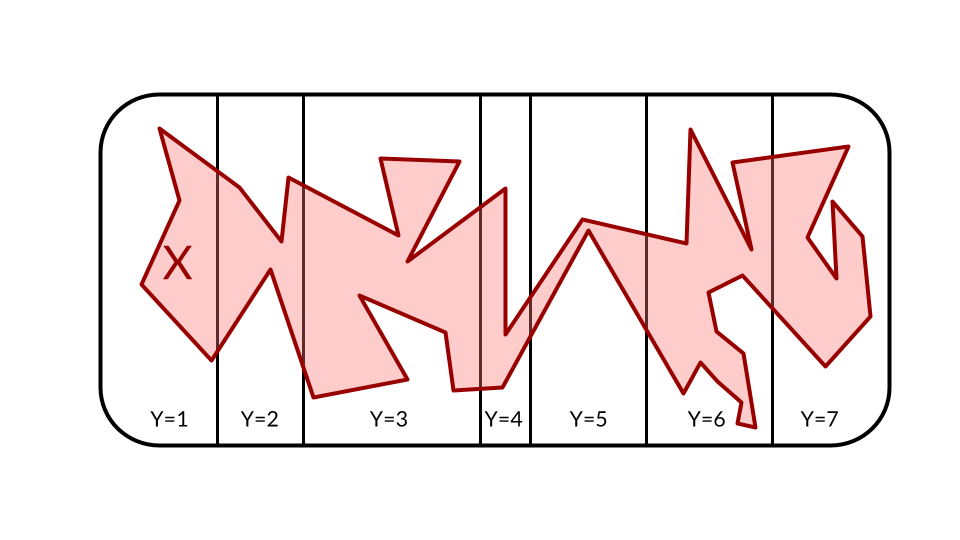
\includegraphics{graphics/ch5-basic-partition.png}

}

\end{figure}%

Taking this argument and encoding it with mathematical notation we get
that
\[P(X=x) = \sum_{y\in\mathcal{Y}} P(X=x, Y=y) \implies p_X(x) = \sum_{y\in\mathcal{Y}} p_{X,Y}(x,y).\]
The process of marginalization involves summing over one of the random
variables in a joint distribution, leaving behind only the marginal of
the other. This is often a very effective way of determining a marginal
distribution when information about two random variables is easier to
discern than information about only one.

To complete the analogy to the law of total probability, recall that the
multiplication rule tells us that \(p_{X,Y}(x,y) = p_{X|Y}(x|y)p_Y(y)\),
and so we may also marginalize by taking
\[p_X(x) = \sum_{y\in\mathcal{Y}} p_{X|Y}(x|y)p_Y(y).\] This makes it
clear that marginalization is often accomplished via arguments based on
conditioning.

\end{tcolorbox}

When confronted with questions from statistics and probability, it will
often be the case that the natural answer to the question is ``it
depends.'' For instance, if asked ``what is the probability that a
student passes their next exam?'' the likely response is ``it depends.''
One very useful technique for solving these questions in a satisfactory
way is to continue that line of thought and explicitly specify ``on
what.'' In the previous example, you may say ``it depends on how much
they study.'' The conceit here is that, if you knew how much the student
studied, then you would better understand the outcomes of the student's
exam.

In mathematical terms this means you have a firm belief about the
conditional distribution between the random quantities of \emph{exam
performance} and \emph{study time}. The process of marginalization, and
the law of total probability before that, provide useful ways of being
able to translate these ``it depends'' statements into concrete beliefs
about the marginal probabilities. Recall that marginal distributions are
distributions which do not depend on any other quantity, and instead,
thy capture the overall behaviour of a random variable. They have, in
some sense, averaged out all other factors and give you the beliefs
which do not depend on anything else at all. The technique for
accomplishing this is marginalization.\footnote{We shall see other forms
  of these ``conditioning arguments'' in the next chapter, where we try
  to summarize the behaviour of a random variable.}

\begin{example}[Photos and Bird Sightings on their
Own]\protect\hypertarget{exm-conditioning}{}\label{exm-conditioning}

Recall that when Charles and Sadie go on their bird watching adventures,
Charles takes photos hoping for as many good ones as possible, and Sadie
spots the birds. We take \(X\) to be the number of good photos taken on
these trips, and \(Y\) to be the number of rare birds that are seen. We
noted that
\[p_{X,Y}(x, y) = \binom{10y}{x}\times(0.25)^{x}\times(0.75)^{10y - x}\times\frac{e^{-3}3^y}{y!},\]
with \(0 \leq x \leq 10y\), and \(y \geq 0\).

\begin{enumerate}
\def\labelenumi{\alph{enumi}.}
\tightlist
\item
  Write down an expression for the marginal probability mass function of
  \(Y\).
\item
  Write down an expression for the marginal probability mass function of
  \(X\).
\item
  \textbf{Challenge:} solve for the marginal probability mass function
  of \(Y\).
\end{enumerate}

\begin{tcolorbox}[enhanced jigsaw, colback=white, breakable, rightrule=.15mm, leftrule=.75mm, toprule=.15mm, left=2mm, arc=.35mm, opacityback=0, bottomrule=.15mm]

\vspace{-3mm}\textbf{Solution}\vspace{3mm}

\begin{enumerate}
\def\labelenumi{\alph{enumi}.}
\item
  To find \(p_Y(y)\), we marginalize over \(X\). That is, we sum the
  joint probability distribution function over all values for \(X\).
  This gives
  \[p_Y(y) = \sum_{x = 0}^{10y} p_{X,Y}(x, y) = \sum_{x = 0}^{10y} \binom{10y}{x}\times(0.25)^{x}\times(0.75)^{10y - x}\times\frac{e^{-3}3^y}{y!}.\]
\item
  To find \(p_X(x)\), we marginalize over \(Y\). That is, we sum the
  joint probability distribution function over all values for \(Y\).
  This gives
  \[p_X(x) = \sum_{y = 0}^{\infty} p_{X,Y}(x, y) = \sum_{y = 0}^{\infty} \binom{10y}{x}\times(0.25)^{x}\times(0.75)^{10y - x}\times\frac{e^{-3}3^y}{y!}.\]
\item
  Note, that you will generally not be expected to manipulate these
  types of sums, however, it is possible to do. First, for \(p_Y(y)\),
  \begin{align*}
  p_Y(y) &= \sum_{x = 0}^{10y} \binom{10y}{x}\times(0.25)^{x}\times(0.75)^{10y - x}\times\frac{e^{-3}3^y}{y!} \\
  &= \frac{e^{-3}3^y}{y!}\underbrace{\sum_{x = 0}^{10y} \binom{10y}{x}\times(0.25)^{x}\times(0.75)^{10y - x}}_{=1} \\
  &= \frac{e^{-3}3^y}{y!}.
  \end{align*}
\end{enumerate}

\end{tcolorbox}

\end{example}

\section{Independent and Identically Distributed: A Framework for
Interpretation}\label{independent-and-identically-distributed-a-framework-for-interpretation}

A very common assumption when addressing questions in statistics and in
probability is that we have a set of random variables which are
independent and identically distributed (often written iid). We now have
the tools to understand concretely what this means.

\begin{definition}[Independent and Identically Distributed
(iid)]\protect\hypertarget{def-iid}{}\label{def-iid}

A set of random variables, \(X_1,X_2,\dots,X_n\) are said to be
independent and identically distributed (denoted iid) whenever:

\begin{enumerate}
\def\labelenumi{\roman{enumi}.}
\tightlist
\item
  every subset of random variables in the collection is independent of
  every other subset of random variables in the collection; and
\item
  the marginal distribution for each of the random variables are exactly
  the same.
\end{enumerate}

\end{definition}

The assumption of iid random quantities will often come up when we are
repeating a process many times over, and thinking about what
observations will arise from this. Suppose that \(X_1\) is a random
variable that takes the value \(1\) if a flipped coin comes up heads,
and \(0\) otherwise. If we imagine flipping this coin \(100\) times then
it is reasonable to assume that each sequential coin flip will be
independent of each other coin flip, since the result on one flip of a
coin should not influence the result of any other flip of a coin.
Moreover, every time the coin is flipped, it is reasonable to assume
that the probability it shows up heads remains the same. As a result,
these \(100\) random quantities, (\(X_1, X_2, \dots, X_{100}\)), are
said to be iid.

\begin{example}[Reframing the Bird
Photos]\protect\hypertarget{exm-iid}{}\label{exm-iid}

Charles and Sadie had, to this point, been considering their bird photo
taking adventures in terms of the joint and conditional distributions.
After learning of independent and identically distributed random
variables, Charles thinks that there is another way to frame the setup,
and describes the following to Sadie:

\begin{quote}
Suppose it is known that there will be \(y\) birds seen on any given
day. Then, the total number of good pictures of birds can be viewed as
the sum of the number of good pictures of each bird. Thus, we can take a
set of iid random variables, say \(X_1,\dots,X_y\) which represent the
number of good pictures taken of each bird.
\end{quote}

\begin{enumerate}
\def\labelenumi{\alph{enumi}.}
\tightlist
\item
  Is this an accurate description? In reality, do we think that this
  will hold?
\item
  Supposing that this description is accurate, and that the probability
  mass function for each \(X_j\) is given by
  \[p_X(x) = \binom{10}{x}(0.25)^{x}(0.75)^{10-x},\] what is the joint
  probability mass function of \((X_1,\dots,X_y)\)?
\end{enumerate}

\begin{tcolorbox}[enhanced jigsaw, colback=white, breakable, rightrule=.15mm, leftrule=.75mm, toprule=.15mm, left=2mm, arc=.35mm, opacityback=0, bottomrule=.15mm]

\vspace{-3mm}\textbf{Solution}\vspace{3mm}

\begin{enumerate}
\def\labelenumi{\alph{enumi}.}
\item
  Yes, this is a reasonable explanation. In this case, if Charles is
  willing to assume that good photos for one bird do not impact the
  chances of good photos of another bird, then this is a perfectly valid
  way to frame the setting. Note that in this case, \(Y=y\) is still
  random, so this whole description is conditioning on knowing \(Y=y\).
  In the real world, it is likely that photos may not actually be
  independent. If Charles takes some really bad photos of one bird, that
  may impact the chances of taking good photos of the next. However, it
  is likely close enough to correct in order to be true.
\item
  Recall that for independent random variables, the joint probability
  mass function is given by the product of the marginal probability mass
  functions. To simplify the notation, we will define
  \(T(X) = \sum_{i=1}^y x_i\). Thus the probability mass function of
  \(X_1,\dots,X_y\) is given by \begin{align*}
   p_{X_1,X_2,\dots,X_y}(x_1,\dots,x_y) &= \prod_{i=1}^y \binom{10}{x_i}(0.25)^{x_i}(0.75)^{10-x_i} \\
   &= \left(\prod_{i=1}^y\binom{10}{x_i}\right)\times(0.25)^{\sum_{i=1}^y x_i}(0.75)^{10y - \sum_{i=1}^yx_i} \\
   &= \left(\prod_{i=1}^y \frac{10!}{x_i!(10-x_i)!}\right)\times 0.25^{T(X)}\times 0.75^{10y - T(X)} \\
   &= \left(\frac{(10!)^y}{\prod_{i=1}^y x_i!(10 - x_i)!}\right)\times 0.25^{T(X)}\times 0.75^{10y - T(X)}.
  \end{align*}
\end{enumerate}

\end{tcolorbox}

\end{example}

While we will use the assumption of iid random variables explicitly at a
later point.The iid assumption also provides an intuitive method for
interpreting probability functions and distributions.

Suppose that we were to take a probability mass function, \(p_X(x)\). If
we were able to generate independent and identically distributed
realizations from this probability mass function, then the function
\(p_X(x)\) describes the behaviour for these repeated realizations.
Specifically, \(p_X(x)\) will give the long-run proportion of
realizations of the iid random variables which take the value \(x\).

This type of statement is always the flavour of interpretation
statements that are made with respect to probability and statistics. It
is always be the case that, in order to understand what is meant by a
statement of probability, we consider the repetition of some statistical
experiment over and over again. When we were discussing sample spaces
and experiments directly, we talked about repeating the experiment over
and over again. When we begin to work with random variables instead, it
becomes more natural to think about the replication procedures coming
through the use of independent and identically distributed random
variables.

As your study of probability progresses, you will begin to work with
random quantities in a strictly theoretical sense. In introductory level
problems, we are often holding in mind very concrete examples to
illustrate the procedures and concepts. In this setting it is easy
enough to hold in mind the experiment of interest: for instance, we may
have a random variable representing the result of a coin toss, and you
can envision repeatedly tossing a coin. As the concepts become less
concrete, more abstract, and harder to draw direct parallels to tangible
scenarios, it becomes more and more important to rely on the
interpretations rooted in a series of independent and identically
distributed random variables.

A large component of statistics as an area of study is making explicit
the assumptions we are working with, and doing our best to ensure that
these are reasonable. By interpreting probability mass functions as the
proportion of independent and identically distributed random variables
that take on a particular value when we repeatedly take realizations of
these random variables, this philosophy is made clear and explicit.

\chapter{The Expected Value and Location
Summaries}\label{the-expected-value-and-location-summaries}

\section{Summarizing the Location of a
Distribution}\label{summarizing-the-location-of-a-distribution}

Until this point in our discussions of probability we have relied upon
characterizing the behaviour of a random variable via the use of
probability mass functions. In some sense, a probability mass function
captures all of the probabilistic behaviour of a discrete random
variable. Using the mass function you are able to characterize how
often, in the long run, any particular value will be observed, and
answer any questions associated with this. As a result, the mass
function remains a critical area of focus for understanding how random
quantities behave.

However, these functions need to be explored and manipulated in order
for useful information to be extracted from them. They do not summarize
this behaviour effectively, as they are not intended to be a summary
tool. We may wish to have numeric quantities which are able to
\emph{concisely} express the behaviour of a distribution. Put
differently, provided with a probability mass function it is hard to
immediately answer ``what do we expect to happen with this random
variable?'' despite the fact that this is a very obvious first question.

To address questions related to our expectations, we turn towards the
statistical concept of central tendency or location.

\begin{definition}[Location (Central
Tendency)]\protect\hypertarget{def-location}{}\label{def-location}

The location of a distribution is a measure of a typical value, or a
central value, for that distribution. A measure of location may also be
referred to as a measure of central tendency.

\end{definition}

With measures of location we are trying to capture, with one single
number, what value is expected when we make observations from the random
quantity. There are many ways one might think to describe our
expectations, and it is worth exploring these concepts in some detail.
In particular, we want to explore how we might think to define the
\textbf{expected value} of a distribution.\footnote{As a general rule
  when learning it is often helpful to consider exercises of discovery.
  That is, try to determine \emph{why} particular definitions are the
  way that they are, or where they have from.}

\section{Deriving the Expected Value}\label{deriving-the-expected-value}

\subsection{The Mode}\label{the-mode}

One way that we may think to define our expected value is by asking what
value is the most probable. This is a question which can be directly
answered using the probability mass function. The process for this
requires looking at the function and determining which value for \(x\)
corresponds to the highest probability. This is the value that we are
most likely to see. Sometimes this procedure is fairly straightforward,
sometimes it is quite complicated. Regardless of the complexity of the
specific scenario, the most probable value has a straightforward
interpretation. As intuitive as this may seem, this is not the value
that will be used as \emph{the} expected value generally. Instead, this
quantity is referred to as the mode.

\begin{definition}[Mode]\protect\hypertarget{def-mode}{}\label{def-mode}

The mode of a distribution is the most probable value of that
distribution. Specifically, if \(X\) is a discrete random variable with
mass function \(p_X(x)\), then the mode is the value of \(x\) such that
\(p_X(x)\) is maximized.

\end{definition}

\begin{example}[Charles and Sadie Investigate Cupcake
Sprinkles]\protect\hypertarget{exm-mode}{}\label{exm-mode}

Charles and Sadie have noticed that their favourite coffee shop has been
experiencing less foot traffic ever since \emph{Probability Patisserie:
Cupcake Conundrums} has opened up next door.\footnote{You should picture
  the owner of this fictitious cupcake store as a giant, multinational,
  faceless corporation. A corporation that seems to take pleasure in
  stepping on the local businesses. That way, as Charles and Sadie try
  to fight back, we can remain on their side!} This cupcake shop has
been attracting many of the regular customers, though, Charles and Sadie
think that it has more to do with fancy marketing than with a better
product. To this end, they go into the store and workout the probability
mass function for \(X\), the number of sprinkles on top of the cupcakes.
They find the following
\[p_X(x) = \begin{cases} 0.25 & x = 0 \\ 0.3 & x = 1 \\ 0.1 & x = 2 \\ 0.05 & x \in \{3,4,5,6,7,8,9\} \\ 0 & \text{otherwise}.\end{cases}\]

What is the mode for the number of sprinkles on the cupcakes?

\begin{tcolorbox}[enhanced jigsaw, colback=white, breakable, rightrule=.15mm, leftrule=.75mm, toprule=.15mm, left=2mm, arc=.35mm, opacityback=0, bottomrule=.15mm]

\vspace{-3mm}\textbf{Solution}\vspace{3mm}

The mode is the value \(x\) such that \(p_X(x)\) is a maximum. In this
case the maximum occurs when \(x=1\), with \(p_X(1) = 0.3\), and so the
mode of the number of sprinkles is \(1\).

\end{tcolorbox}

\end{example}

While the mode is a useful quantity, and for some decisions will be the
most relevant summary value, there are some major issues with it as a
general measure of location. For starters, consider that our most common
probability model considered until this point has been that of equally
likely outcomes. Here, there is no well-defined mode.\footnote{When
  multiple modes exist, convention tends to report the set of all of the
  modes. In the equally likely outcome model, this is the entire support
  for the random variable, and as a result, the mode is exactly the
  probability mass function. There is no summary provided.} While the
case of equally likely outcomes is a fairly strong example highlighting
the issues with the mode, it need not be so dramatic to undermine its
utility. It is possible for a distribution to have several modes which
are quite distinct from one another, even if it's not all values in the
support.

Moreover, it is quite common for the modal value to be not particularly
likely itself. Consider a random variable that can take on a million
different values. If all of the probabilities are approximately
\(0.000001\) then presenting the mode as the most probable value does
not translate to saying that the mode is particularly probable.

\begin{example}[Charles and Sadie Investigate Cupcake
Happiness]\protect\hypertarget{exm-triangular-distributions}{}\label{exm-triangular-distributions}

After realizing that the cupcake shop did not provide very many
sprinkles, Charles and Sadie decided to turn to the marketing material.
In it, \emph{Cupcake Conundrums} claims that, on a scale from \(0\) to
\(100,000\) happiness points, most of their customers experience the
maximum happiness after eating their cupcakes. Charles and Sadie are
well aware of the ways in which these types of reports can be
misleading, and so they investigate, finding the following probability
mass function for the number of happiness points.
\[p_X(x) = \begin{cases}
    \frac{x}{5,000,050,000} & x \in \{1,\dots,100 000\} \\
    0 & \text{otherwise}.
\end{cases}\]

\begin{enumerate}
\def\labelenumi{\alph{enumi}.}
\tightlist
\item
  Is the mode reported by the company correct?
\item
  Is the mode an accurate depiction of the distribution in this setting?
\end{enumerate}

\begin{tcolorbox}[enhanced jigsaw, colback=white, breakable, rightrule=.15mm, leftrule=.75mm, toprule=.15mm, left=2mm, arc=.35mm, opacityback=0, bottomrule=.15mm]

\vspace{-3mm}\textbf{Solution}\vspace{3mm}

\begin{enumerate}
\def\labelenumi{\alph{enumi}.}
\item
  Yes. Note that \(p_X(x)\) is increasing in \(x\). As a result, the
  mode of the distribution is the highest value that the distribution
  can take on, which in this case is \(x = 100,000\).
\item
  The mode is likely not a good indication of the distribution. Note
  that the maximal value happens only \(100000/5000050000\) of the time,
  which is a very very small value. If you look at the probability that
  a customer is only halfway happy, this is \(50000/5000050000\). This
  value is half the likelihood of the modal value, but the difference
  between these two probabilities is also only
  \(50000/5000050000 \approx 0.000001\). That is, it is only \(1\) in
  \(100,000\) more likely to observe perfect happiness compared with
  half happiness. By extension, it is only about \(2\) in \(100,000\)
  more likely to observe perfect happiness compared with no happiness.
  The mode simply is not a good indicator of behaviour in this setting.
\end{enumerate}

\end{tcolorbox}

\end{example}

\subsection{The Median}\label{the-median}

If the mode has these shortcomings, what else might work? Another
intuitive concept is to try to select the ``middle'' of the
distribution. One way to define the middle would be to select the value
such that, in the long run, half of observations from the distribution
are beneath it and half are above it. That way, when you are told this
value, you immediately know that it is equally likely to observe values
on either side of this mark. This is also a particularly intuitive
definition for expected value, and is important enough to be named, the
median.

\begin{definition}[Median]\protect\hypertarget{def-median}{}\label{def-median}

The median of a distribution is the value \(m\) which attempts to have
\(P(X \leq m) = 0.5\) and \(P(X \geq m) = 0.5\). This value may not
always exist, and so formally for discrete random variables, the median
\(m\) is any value such that \(P(X \leq m) \geq 0.5\) and
\(P(X \geq m) \geq 0.5\).

\end{definition}

The median is the midpoint of a distribution and is very important for
describing the behaviour of random variables. Medians are often the most
helpful single value to report to indicate the typical behaviour of a
distribution, and they are frequently used. When people interpret
averages it is often the median that they are actually interpreting. It
is very intuitive to be given a value and know that half of all
realizations are above that point, and half of all realizations are
below that point.

\begin{example}[Charles and Sadie Investigate Cupcake Sprinkles
(Again)]\protect\hypertarget{exm-median}{}\label{exm-median}

After seeing how the cupcake shop used the mode to misrepresent the
happiness of its customers, Charles and Sadie worry that they may have
been unfair with using the mode. As a result, they turn back to the
cupcake sprinkle distribution and try to summarize it differently.
Recall that the probability mass function for \(X\), the number of
sprinkles on top of the cupcakes, is
\[p_X(x) = \begin{cases} 0.25 & x = 0 \\ 0.3 & x = 1 \\ 0.1 & x = 2 \\ 0.05 & x \in \{3,4,5,6,7,8,9\} \\ 0 & \text{otherwise}.\end{cases}\]

What is the median number of sprinkles on the cupcakes?

\begin{tcolorbox}[enhanced jigsaw, colback=white, breakable, rightrule=.15mm, leftrule=.75mm, toprule=.15mm, left=2mm, arc=.35mm, opacityback=0, bottomrule=.15mm]

\vspace{-3mm}\textbf{Solution}\vspace{3mm}

Note that we are looking for a value, \(m\), such that
\(P(X \geq m) \geq 0.5\) and \(P(X \leq m) \geq 0.5\). To find this we
can consider the cumulative probability sums. We know that
\(P(X \leq k) = \sum_{x=0}^k p_X(x)\), and as a result, stopping this
value at the first time that the sum goes beyond \(0.5\) satisfies the
second condition. In this case our cumulative sums are \(0.25\) then
\(0.55\). As a result, \(P(X \leq 1) = 0.55 > 0.5\). If we check
\(P(X \geq 1) = 1 - P(X < 1) = 1 - P(X = 0) = 0.75 > 0.5\). As a result,
\(m=1\) satisfies the required conditions and is a median.

\end{tcolorbox}

\end{example}

Despite the advantages of medians, they have their own drawbacks. For
starters, the median can be exceptionally challenging to compute in
certain settings. As a result, even when a median is appropriate, it may
not be desirable if it is too challenging to determine.

Beyond the difficulties in computation, medians have a feature which is
simultaneously a major benefit and a major drawback. Specifically,
medians are less influenced by extreme values in the probability
distribution. Consider two different distributions. The first is equally
likely to take any value between \(1\) and \(10\). The second is equally
likely to take any value between \(1\) and \(9\) or \(1,000,000\). In
both of these settings, the median is \(5\) since \(P(X\leq 5) = 0.5\)
and \(P(X \geq 5) = 0.5\). However, in the second setting we may observe
a value as high as \(1,000,000\). Moreover, this value will be observed
as often as the median will be.

The median, in some sense, ignores the extreme value in the probability
distribution. In certain settings, this can be very
desirable.\footnote{You will find many introductory sources that say
  that you should always use the median when you are concerned with
  extreme values. This is a great oversimplification of the truth, and
  points to a general rule in Statistics: there are very few general
  rules. The guidance comes from the fact that often extreme values skew
  our perceptions of the underlying truth. While this may be true in
  general, it is not true often enough to warrant being given as
  universal guidance.} Consider the distribution of household incomes.
There are a few households that earn an incredibly large amount,
compared to the remaining households. If you are interested in
understanding the ``average household'', the median may be a more
appropriate measure, as those households with extreme incomes would
otherwise distort the picture provided by most families. In this sense,
the median's robustness to extreme values is a positive feature of it in
terms of a summary measure for distributional behaviour.

Suppose instead that you work for an insurance company and are concerned
with understanding the value of insurance claims that your company will
need to pay out. The distribution will look quite similar to the income
distribution. Most of the probability will be assigned to fairly small
claims, with a small chance of a very large one. As an insurance
company, if you use the median this large claim behaviour will be
smoothed over, perhaps leaving you unprepared for the possibility of
extremely large payouts. In this setting, the extreme values are
informative and important, and as a result the median's robustness
becomes a hindrance to correctly describing the important
behaviour.\footnote{An insurance company ignoring these massive claims
  would almost certainly go out of business very, very quickly.}

\begin{example}[Charles and Sadie Investigate Cupcake Public
Relations]\protect\hypertarget{exm-median-two}{}\label{exm-median-two}

Charles and Sadie feel as though they may be finally catching a break
when word gets around that the cupcake shop was using spoiled
ingredients, making the patrons sick! The cupcake shop, in hearing this,
sent their massive public relations team into damage control mode. They
claimed that the median number of illnesses per week associated with the
cupcake store was the same as most local food services businesses. Doing
some digging, Charles and Sadie find the following two probability mass
functions, for \(X\) and \(Y\), where \(X\) is the number of weekly
illnesses at the cupcake shop, and \(Y\) is the number from a local
business that has been around for a while. \begin{align*}
p_X(x) &= \begin{cases}
    0.1 & x = 0 \\ 
    0.1 & x = 1 \\
    0.35 & x = 2 \\
    0.05 & x = 3 \\ 
    0.4 & x = 25 \\
    0 & \text{otherwise};
\end{cases} \\
p_Y(y) &= \begin{cases}
    0.45 & x = 0 \\
    0.04 & x = 1 \\
    0.5 & x = 2 \\
    0.01 & x = 3
\end{cases}.
\end{align*}

\begin{enumerate}
\def\labelenumi{\alph{enumi}.}
\tightlist
\item
  What is the median of \(X\)?
\item
  What is the median of \(Y\)?
\item
  Is the claim made by the public relations team an accurate depiction
  of the world? Why or why not?
\end{enumerate}

\begin{tcolorbox}[enhanced jigsaw, colback=white, breakable, rightrule=.15mm, leftrule=.75mm, toprule=.15mm, left=2mm, arc=.35mm, opacityback=0, bottomrule=.15mm]

\vspace{-3mm}\textbf{Solution}\vspace{3mm}

\begin{enumerate}
\def\labelenumi{\alph{enumi}.}
\item
  We can consider cumulative sums here again. In order we get, \(0.1\),
  \(0.2\), \(0.55\). This suggests that \(x=2\) is a candidate. If we
  check \(P(X \geq 2) = 1 - 0.2 = 0.8\), and so \(x=2\) is a median.
\item
  Using cumulative sums we get \(0.45\), \(0.49\), \(0.99\). Again, this
  gives \(x=2\) as a candidate. If we check
  \(P(X \geq 2) = 1 - 0.49 = 0.51\), and so \(x=2\) is a median.
\item
  The claim is accurate in that the median number for both
  establishments in \(2\). However, here the median is a bad
  representation for \(X\). The probability that more than \(2\) cases
  occur in a week at the cupcake shop is \(0.8\), compared with \(0.51\)
  at the local business. What's more, the probability that \(X\) is as
  high as \(25\) is \(0.4\), where \(Y\) is \emph{never} higher than
  \(3\).
\end{enumerate}

\end{tcolorbox}

\end{example}

Between the median and the mode we have two measures which capture some
sense of expected value, each with their own set of strengths and
drawbacks. Neither capture what it is that is referred to as \emph{the}
expected value. For this, we need to take inspiration from the median,
and consider another way that we may think to find the center of the
distribution.

\subsection{The Mean}\label{the-mean}

If the median gives the middle reading along the values sequentially, we
may also wish to think about trying to find the \emph{center of gravity}
of the numbers. Suppose you take a pen, or marker, or small box of
chocolates, and you wish to balance this object on a finger or an arm.
To do so, you do not place the item so that half of its length sits on
one side of the appendage and half on the other. You adjust the location
so that half of the \emph{mass} sits on either side of the appendage.

Throughout our discussion of discrete random variables we have referred
to probability as \emph{mass}. We use the \emph{probability mass
function} to generate our probability values. This metaphor can be
extended when we try to find the center of the distribution. If we
imagine placing a mass with weight equal to the probability mass at each
value that a random variable can take on, we may ask, ``where would we
have to place a fulcrum to have this number line be balanced?'' The
answer to this question serves as another possible measure of center. It
turns out that this notion of center is the one that we are all most
familiar with, the simple average, or mean.

\begin{definition}[Mean]\protect\hypertarget{def-mean}{}\label{def-mean}

The mean of a distribution is the center of mass of the distribution.
For a random variable, \(X\) with support \(\mathcal{X}\), and
probability mass function \(p_X(x)\), the mean of \(X\) is given by
\[\sum_{x \in \mathcal{X}} xp_X(x).\]

\end{definition}

It is this measure of location which ends up being called the
\textbf{expected value} in statistics. We will use average, expected
value, mean, and expectation interchangeably. In terms of notation, the
expected value of a random variable \(X\) is denoted \(E[X]\).
Mathematically, the expected value is desirable for many reasons, some
of which we will study in more depth later on. One of these desirable
features, which stands in contrast with the median, is the comparative
ease with which expected values can be computed. The summation for the
expected value is easy to write down, and typically can be solved
(either analytically, or readily with a computer).

\begin{example}[Charles and Sadie Investigate Cupcake Sprinkles (One
Last
Time)]\protect\hypertarget{exm-expected-value-one}{}\label{exm-expected-value-one}

While the median and mode number of sprinkles on the cupcakes were the
same, Charles and Sadie realize that this does not end up connecting
well with the total number of sprinkles given out. Perhaps customers
like the possibility of getting a large number of sprinkles, if they get
lucky. As a result, they decide to round out the summary of the
distribution by considering the mean number of sprinkles as well. Recall
that the probability mass function for \(X\), the number of sprinkles on
top of the cupcakes, is
\[p_X(x) = \begin{cases} 0.25 & x = 0 \\ 0.3 & x = 1 \\ 0.1 & x = 2 \\ 0.05 & x \in \{3,4,5,6,7,8,9\} \\ 0 & \text{otherwise}.\end{cases}\]

What is the mean number of sprinkles?

\begin{tcolorbox}[enhanced jigsaw, colback=white, breakable, rightrule=.15mm, leftrule=.75mm, toprule=.15mm, left=2mm, arc=.35mm, opacityback=0, bottomrule=.15mm]

\vspace{-3mm}\textbf{Solution}\vspace{3mm}

Recall that the mean of a distribution is given by
\(E[X] = \sum_{x\in\mathcal{X}}xP_X(x)\). In this case, this results in
\begin{align*}
    &\sum_{x=0}^9 xp_X(x) \\
    &= 0(0.25) + 1(0.3) + 2(0.1) + (3+4+5+6+7+8+9)(0.05) \\
    &= 2.6.
\end{align*} As a result, the mean number of sprinkles used is \(2.6\).
This is higher than the median and mode, but is still not particularly
high.

\end{tcolorbox}

\end{example}

In the case of an equally likely probability model, the expected value
becomes the standard average that is widely used. Suppose that there are
\(n\) options in the support with \(\mathcal{X} = \{x_1,\dots,x_n\}\).
We can write
\[E[X] = \sum_{i=1}^n x_i\frac{1}{n} = \frac{1}{n}\sum_{i=1}^nx_i.\]
This is the formula for the average that is most commonly applied. When
the probability models are more complex, the formula is not precisely
the standard average -- instead, it becomes a weighted average, where
the weights are the probabilities.\footnote{While less commonly applied
  than the simple average, a weighted average is familiar to most
  students for a crucial purpose: grade calculations. If you view the
  weight of each item in a course as a probability mass, and the grade
  you scored as the value, then your final grade in the course is
  exactly the expected value of this distribution.} The frequency with
which expected values are used make them attractive as a quick summary
for the center of a distribution.

\subsection{How is the Mean
``Expected''?}\label{how-is-the-mean-expected}

While the mean provides a useful, intuitive measure of center of the
distribution, it is perhaps counterintuitive to name it the ``expected
value.'' To understand the naming convention it is easiest to consider
the application which has likely spurred more development of statistics
and probability than any other: gambling.

Suppose that there is some game of chance that can pay out different
amounts with different probabilities. A critical question for a gambler
in deciding whether or not to play such a game is ``how much can I
expect to earn, if I play?'' This is crucial to understanding, for
instance, how much you should be willing to pay to participate, or if
you are the one running the game, how much you should charge to ensure
that you make a profit.

If you want to understand what you expect to earn, the intuitive way of
accomplishing this is to weight each possible outcome by how likely it
is to occur. This is exactly the expected value formula that has been
provided, and so the expected value can be thought of as the expected
payout of a game of chance where the outcomes are payouts corresponding
to each probability.

\begin{tcolorbox}[enhanced jigsaw, rightrule=.15mm, leftrule=.75mm, opacitybacktitle=0.6, title={Cost for a Game of Chance}, colframe=quarto-callout-tip-color-frame, opacityback=0, coltitle=black, breakable, toptitle=1mm, colbacktitle=quarto-callout-tip-color!10!white, bottomtitle=1mm, titlerule=0mm, arc=.35mm, colback=white, toprule=.15mm, left=2mm, bottomrule=.15mm]

Suppose that a game of chance is being run. It will cost \(\$m\) to
play, and the game will pay out values from \(\mathcal{X}\), according
to a random variable \(X\) with probability mass function \(p_X(x)\).
The question that we want to know is what should the value be for \(m\),
such that, in the long term, a player playing the game will earn no
money?

Note that if \(X=x\) then a player playing the game will earn \(x - m\)
for that play, and this will happen with probability \(p_X(x)\). Thus,
in the long run, in \(p_X(x)\) proportion of games the player earns
\(x-m\). If the player plays \(N\) games, then as \(N\to\infty\), the
total contribution from these winnings will be
\((x-m)\cdot N\cdot p_X(x)\). If we add up this contribution for all
possible results, \(x\), we get \begin{align*}
\sum_{x\in\mathcal{X}} N(x-m)p_X(x) &= N\left[\sum_{x\in\mathcal{X}}xp_X(x) - \sum_{x\in\mathcal{X}} mp_X(x)\right] \\
&= N\left[\sum_{x\in\mathcal{X}}xp_X(x) - m\sum_{x\in\mathcal{X}}p_X(x)\right] \\
&= N\left[E[X] - m\right].
\end{align*} Thus, in the long run, the total that the player wins, as
\(N\to\infty\) will be \(N(E[X] - m)\). Thus, in order for the long run
earnings to be zero, \(m\) should be set to be equal to \(E[X]\).

If \(m\) is set to be \(0\), then per game the player \emph{expects} to
earn \(E[X]\). This also represents the cost at which a rational actor
should be willing to pay to participate. If a game of chance costs more
than the expected value to play, in the long run you will lose money. If
a game of chance costs less than the expected value, in the long run you
will earn money. It is hard to overstate the utility of gambling in
developing probability theory, and as such these types of connections
are expected.

\end{tcolorbox}

To interpret the expected value of a random variable, one possibility is
using the intuition that we used to derive the result. Notably, the
expected value is the center of mass of the distribution, where the
masses correspond to probabilities. This means that it is not
necessarily an actual central number over the range, but rather that it
sits in the weighted middle. While this interpretation is useful in many
situations, there are times where the point of balance is a less
intuitive description. For these, it can sometimes be useful to frame
the expected value as the long term simple average from the
distribution.

If we imagine observing many independent and identically distributed
random variables, then as the number of samples tends to infinity, the
expected value of \(X\) and the simple average will begin to coincide
with one another. That is the distance between \(E[X]\) and
\(\frac{1}{n}\sum_{i=1}^n X_i\) will shrink to \(0\). As a result, we
can view the expected value as the average over repeated experiments.
This interpretation coincides nicely with the description based on games
of chance. Specifically, if you were to repeatedly play the same game of
chance, the average payout per game will be equal to the expected value,
if you play for long enough.

\begin{figure}[H]

\caption{\label{fig-plot}This plot produces 50000 realizations of the
random variable described in Example~\ref{exm-expected-value-one}. As
computed in the example, the expected value is 2.6. As many repeated
observations are averaged, the empirical average converges to this
computed value.}

\centering{

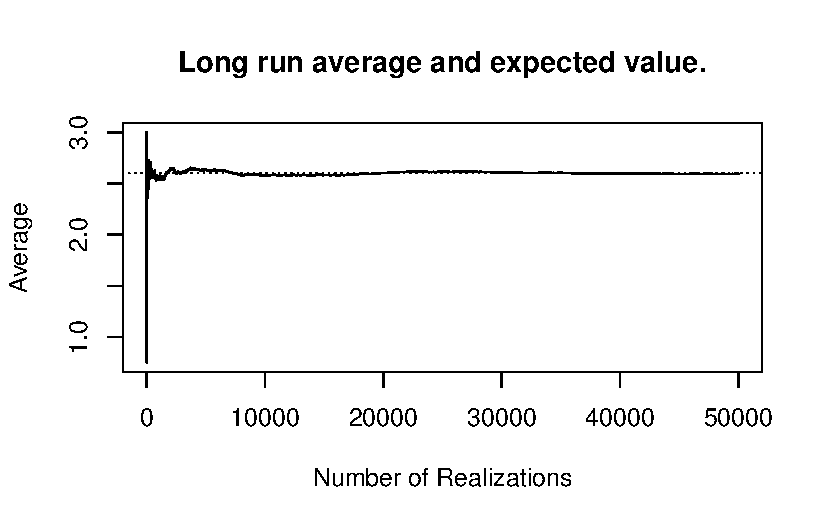
\includegraphics{notes/chapter6_files/figure-pdf/fig-plot-1.pdf}

}

\end{figure}%

\section{Which Measure of Central Tendency Should be
Used?}\label{which-measure-of-central-tendency-should-be-used}

Where the median demonstrated robustness against extreme values in the
distribution, the mean does not. For instance, if we consider the
distribution of incomes across a particular region, the mean will be
much higher than the median, since those families with exceptionally
high incomes will not be smoothed over as they were with medians. In
this case, the lack of robustness for the expected value will render the
mean a less representative summary for the true behaviour of the random
quantity.

To see this concretely consider a random variable which with equal
probability takes a value between \(1\) and \(9\). This will have
\(E[X] = 5\). Now, if the \(9\) is made to be \(1,000,000\), the
expected value will now be \(E[X] = 111115.\dot1\). This is a far cry
from the median which does not change from \(5\) in either case. This
lack of robustness is desirable in the event of the insurance example
from the median discussion, but will be less desirable in other
settings.

The mean, median, and mode are the three standard measures of central
tendency. They are single values which describe the standard behaviour
of a random quantity. Each of the three has merits as a measure, and
each has drawbacks for certain settings. The question of which to use
and when depends primarily on the question of interest under
consideration, rather than on features of the data alone.\footnote{The
  data is one consideration for which measure to use, but not the only
  one (and not the most important one).} Often, presenting more than one
measure can give a better sense of the distributional behaviour that any
one individual will.

\begin{example}[Charles and Sadie Reflect on the Cupcake
Adventures]\protect\hypertarget{exm-choosing-measure-of-central-tendency}{}\label{exm-choosing-measure-of-central-tendency}

Charles and Sadie decide it is worth stepping back and summarizing all
that has happened with regards to their cupcake adventures, trying to
ensure that distributions are always summarized fairly.

\begin{enumerate}
\def\labelenumi{\alph{enumi}.}
\tightlist
\item
  For the number of sprinkles per cupcake is the mean, median, or mode
  the best measure of central tendency?
\item
  For the amount happiness in customers, is the mean, median, or mode
  the best measure of central tendency?
\item
  For the number of customers who become ill eating at establishments,
  is the mean, median, or mode the best measure of central tendency?
\end{enumerate}

\begin{tcolorbox}[enhanced jigsaw, colback=white, breakable, rightrule=.15mm, leftrule=.75mm, toprule=.15mm, left=2mm, arc=.35mm, opacityback=0, bottomrule=.15mm]

\vspace{-3mm}\textbf{Solution}\vspace{3mm}

\begin{enumerate}
\def\labelenumi{\alph{enumi}.}
\item
  There is an argument that any of the measures here could work the
  best, it would depend on the individual's preferences. The mode makes
  a lot of sense as, if you are a regular customer, the mode is what you
  will experience day-to-day; most days you will have the modal number
  of sprinkles. The median may make sense as it provides a benchmark for
  measuring what constitutes a lot of sprinkles and a little. Half of
  the time you'll end up with a more sprinkled donut, half the time a
  less. The mean would be particularly interesting to note for the store
  owners themselves, since the mean is directly tied to totals: if the
  store knows that they sell \(100\) cupcakes per day, most days, then
  they also can expect to use \(100\) times the mean number of sprinkles
  in a day. This is helpful for planning.
\item
  The median is likely the most useful measure in this setting. The mode
  could be useful if happiness were not measured on a \(100,000\) point
  scale. The mean is likely a less relevant value here as we are not
  particularly concerned with the total happiness, and if there was a
  large skew or major outliers in this distribution, we would want to
  determine where the majority fall. This is more analogous to the
  income example rather than the insurance example.
\item
  In this case either the mode or mean are likely the best gauges. Here
  we do care about totals, and in particular, we do not want to smooth
  over outliers. It is very relevant if sometimes a lot of individuals
  become ill after eating an establishment, and the median would hide
  this information.
\end{enumerate}

\end{tcolorbox}

\end{example}

Despite the utility of all three measures, the expected value holds a
place of more central importance in probability and statistics. A lot of
this has to do with further mathematical properties of the mean. Because
of its central role, it is worth studying the expected value in some
more depth.

\section{Expected Values of Functions of Random
Variables}\label{expected-values-of-functions-of-random-variables}

Sometimes the value of a random variable needs to be mapped through a
function to give the value which is most relevant to us. Consider, for
instance, a situation wherein the side lengths of boxes being
manufactured by a specific supplier are random, due to incorrectly
calibrated tolerances in the machines. The resulting boxes are perfect
cubes. Suppose we are interested in the volume of the produced box not
the side length. If a box has side length \(x\), then its volume will be
\(x^3\), and so we may desire some way of computing \(E[X^3]\) rather
than \(E[X]\).

Generally, for a function \(g(X)\), we may want to compute \(E[g(X)]\).
It is important to recognize that \(E[g(X)] \neq g(E[X])\). This is a
common mistake.\footnote{and an attractive one, but a mistake
  nonetheless.} If we are unable to apply the function to the expected
value, then the question of how to compute the expected value remains.
Instead of applying the function to overall expected value, instead, we
apply the function to \emph{each} value in the defining relationship for
the expected value. That is,
\[E[g(X)] = \sum_{x\in\mathcal{X}} g(x)p_X(x).\] This is sometimes
referred to as the ``law of the unconscious statistician,'' a name which
may be aggressive enough to help remember the correct way to compute the
expectation.\footnote{Some statisticians dislike this name. I find it to
  be rather cute.}

\begin{tcolorbox}[enhanced jigsaw, rightrule=.15mm, leftrule=.75mm, opacitybacktitle=0.6, title={The Law of the Unconscious Statistician}, colframe=quarto-callout-note-color-frame, opacityback=0, coltitle=black, breakable, toptitle=1mm, colbacktitle=quarto-callout-note-color!10!white, bottomtitle=1mm, titlerule=0mm, arc=.35mm, colback=white, toprule=.15mm, left=2mm, bottomrule=.15mm]

The law of the unconscious statistician (LOTUS) states that, for a
random variable \(X\), if we wish to find \(E[g(X)]\), then we compute
\[E[g(X)] = \sum_{x\in\mathcal{X}} g(x)p_X(x).\]

\end{tcolorbox}

\begin{example}[The Happiness Scale
Inversion]\protect\hypertarget{exm-expected-value-transformation}{}\label{exm-expected-value-transformation}

Charles and Sadie have made really great strides working to protect
their favourite coffee shop from the new cupcake store. One day when
digging through the material more, they realize that the happiness
report produced by the company is even less accurate than they had
originally reported! The company reported the following probability mass
function for happiness points \[p_X(x) = \begin{cases}
    \frac{x}{5,000,050,000} & x \in \{1,\dots,100 000\} \\
    0 & \text{otherwise}.
\end{cases}\] Charles and Sadie track down the source of this expression
and they find that, in fact, this does not measure happiness points at
all. Instead, the number of happiness points is a function of \(X\),
specifically, \(Z = 1/X\).

\begin{enumerate}
\def\labelenumi{\alph{enumi}.}
\tightlist
\item
  What is the expected value of \(X\)? Note, it may be helpful to recall
  that \(\sum_{x=1}^{k} x^2 = \frac{k(k+1)(2k+1)}{6}\).
\item
  What is the expected value of \(Z\)?
\end{enumerate}

\begin{tcolorbox}[enhanced jigsaw, colback=white, breakable, rightrule=.15mm, leftrule=.75mm, toprule=.15mm, left=2mm, arc=.35mm, opacityback=0, bottomrule=.15mm]

\vspace{-3mm}\textbf{Solution}\vspace{3mm}

\begin{enumerate}
\def\labelenumi{\alph{enumi}.}
\item
  Using directly the formula for \(E[X]\) gives \begin{align*}
  E[X] = \sum_{x=1}^{100000} xp_X(x) &= \sum_{x=1}^{100000} x\frac{x}{5000050000} \\
  &= \frac{1}{5000050000}\sum_{x=1}^{100000}x^2 \\
  &= \frac{1}{5000050000}\cdot\frac{100000(100000+1)(2(100000)+1)}{6} \\
  &= 66 667.
  \end{align*}
\item
  Applying the law of the unconscious statistician, gives \begin{align*}
  E[Z] = E[1/X] = \sum_{x=1}^{100000} \frac{1}{x}p_X(x) &= \sum_{x=1}^{100000} \frac{1}{x}\frac{x}{5000050000} \\
  &= \frac{1}{5000050000}\sum_{x=1}^{100000} 1 \\
  &= \frac{100000}{5000050000} \\
  &= \frac{2}{100001}.
  \end{align*}
\end{enumerate}

\end{tcolorbox}

\end{example}

These functions applied to random variables are often thought of as
``transformations'' of the random quantities. For instance, we
\emph{transformed} a side length into a volume. While the law of the
unconscious statistician will apply to any transformation for a random
variable, we can sometimes use shortcuts to circumvent its application.
In particular, when \(g(X) = aX + b\), for constant numbers \(a\) and
\(b\), we can greatly simplify the expected value of the transformation.
To see this note \begin{align*}
E[aX + b] &= \sum_{x\in\mathcal{X}}(ax + b)p_X(x) \\
&= \sum_{x\in\mathcal{X}}axp_X(x) + bp_X(x) \\
&= a\sum_{x\in\mathcal{X}}xp_X(x) + b\sum_{x\in\mathcal{X}}p_X(X) \\
&= aE[X] + b.
\end{align*} That is, in general, we have that
\(E[aX + b] = aE[X] + b\).

This is particularly useful as linear transformations like \(aX+b\)
arise very commonly. For instance, most unit conversions are simple
linear combinations. If a random quantity is measured in one unit then
this result can be used to quickly convert expectations to another.

\begin{example}[Sadie's Trip to
America]\protect\hypertarget{exm-temperature-conversion}{}\label{exm-temperature-conversion}

Sadie has recently returned from a long trip to America. The trip was
long enough that temperatures measured in Fahrenheit started to make
sense. When Sadie and Charles begin to talk about the weather, Charles
brings up the temperature distribution of a possible summer vacation
spot. Unfortunately for Sadie, these temperatures are all in Celsius.
The distribution Charles provides is \[p_X(x) = \begin{cases}
    0.1 & x \in \{10, 11, 12, 13, 14\} \\
    0.05 & x \in \{15, 16, 17, 18, 19, 20, 21, 22, 23, 24\} \\
    0 & \text{otherwise}
\end{cases}\]

\begin{enumerate}
\def\labelenumi{\alph{enumi}.}
\tightlist
\item
  What is the expected temperature, in Celsius?
\item
  Supposing that the temperature in Fahrenheit is given by
  \(Y = 1.8X + 32\), what is the expected temperature in Fahrenheit?
\end{enumerate}

\begin{tcolorbox}[enhanced jigsaw, colback=white, breakable, rightrule=.15mm, leftrule=.75mm, toprule=.15mm, left=2mm, arc=.35mm, opacityback=0, bottomrule=.15mm]

\vspace{-3mm}\textbf{Solution}\vspace{3mm}

\begin{enumerate}
\def\labelenumi{\alph{enumi}.}
\item
  Here we find \begin{align*}
   \sum_{x=10}^{24} xp_X(x) &= 0.1\sum_{x=10}^{14}x + 0.05\sum_{x=15}^{24}x \\
   &= 15.75.
  \end{align*}
\item
  Since \(E[X] = 15.75\) then
  \(E[Y] = E[1.8X + 32] = 1.8E[X] + 32 = 60.35\).
\end{enumerate}

\end{tcolorbox}

\end{example}

This type of linear transformation also frequently comes up with games
of chance and payouts, or with scoring more generally.\footnote{For
  instance, suppose you are betting a certain amount on the results of a
  coin toss, or that you are taking a multiple choice test that gives
  \(2\) points for a correct answer.}

Measures of central tendency are important to summarize the behaviour of
a random quantity. Whether using the mean, median, or mode, these
measures of location describe, on average, what to expect from
observations of the random quantity. However, understanding a
distribution requires understanding far more than simply the measures of
location. As was discussed previously, the probability mass function
captures the complete probabilistic behaviour of a discrete random
variable, it is only intuitive that some information would be lost with
a single numeric summary.

\begin{tcolorbox}[enhanced jigsaw, rightrule=.15mm, leftrule=.75mm, opacitybacktitle=0.6, title={Equal Location Across Different Distributions}, colframe=quarto-callout-warning-color-frame, opacityback=0, coltitle=black, breakable, toptitle=1mm, colbacktitle=quarto-callout-warning-color!10!white, bottomtitle=1mm, titlerule=0mm, arc=.35mm, colback=white, toprule=.15mm, left=2mm, bottomrule=.15mm]

Consider the following three distributions for three random variables,
\(X\), \(Y\), and \(Z\): \begin{align*}
p_X(x) = \begin{cases}
    0.25 & x = -1 \\
    0.5 & x = 0 \\ 
    0.25 & x = 1 \\
    0 & \text{otherwise}.
\end{cases} \quad
p_Y(y) &= \begin{cases}
    0.05 & x = -5 \\
    0.1 & x = -4 \\
    0.1 & x = -3 \\
    0.1 & x = -2\\
    0.1 & x = -1\\
    0.15 & x = 0 \\ 
    0.1 & x = 1\\
    0.1 & x = 2\\
    0.1 & x = 3\\
    0.1 & x = 4 \\
    0.05 & x = 5 \\
    0 & \text{otherwise}.
\end{cases} \quad
p_Z(z) = \begin{cases}
    0.25 & x = -400 \\
    0.5 & x = 0 \\
    \frac{1}{3196} & x \in \{1,\dots,799\}\\
    0 & \text{otherwise}.
\end{cases}.
\end{align*}

In each of these distributions we have the mean, median, and mode all
equalling \(0\).\footnotemark{} However, even just from a quick glance,
these distributions are all very, very differently behaved. The location
summaries here clearly miss much of the important information about
these different distributions. Spend some time trying to think of the
ways in which they differ from one another, and see if you can determine
\emph{what} is missing from relying solely on measures of location.

\end{tcolorbox}

\footnotetext{Try working this out!}

\part{Part 2: Statistics}

\phantomsection\label{refs}
\begin{CSLReferences}{1}{0}
\bibitem[\citeproctext]{ref-fairCoin}
Bartoš, František, Alexandra Sarafoglou, Henrik R. Godmann, Amir
Sahrani, David Klein Leunk, Pierre Y. Gui, David Voss, et al. 2023.
{``Fair Coins Tend to Land on the Same Side They Started: Evidence from
350,757 Flips.''} \url{https://arxiv.org/abs/2310.04153}.

\bibitem[\citeproctext]{ref-rainPaper}
Gigerenzer, Gerd, Ralph Hertwig, Eva Van Den Broek, Barbara Fasolo, and
Konstantinos V Katsikopoulos. 2005. {``{`A 30\% Chance of Rain
Tomorrow'}: How Does the Public Understand Probabilistic Weather
Forecasts?''} \emph{Risk Analysis: An International Journal} 25 (3):
623--29.

\bibitem[\citeproctext]{ref-kahneman}
Kahneman, Daniel, and Amos Tversky. 1972. {``Subjective Probability: A
Judgment of Representativeness.''} \emph{Cognitive Psychology} 3 (3):
430--54.

\end{CSLReferences}



\end{document}
